% =============================================================================
% Moon Recognition — Lunar Surface Feature Segmentation
% Author: Giancarlo Venturato
% LCP (Laboratory of Computational Physics) 2026 — Group 2614
%
% Usage: % =============================================================================
% Moon Recognition — Lunar Surface Feature Segmentation
% Author: Giancarlo Venturato
% LCP (Laboratory of Computational Physics) 2026 — Group 2614
%
% Usage: % =============================================================================
% Moon Recognition — Lunar Surface Feature Segmentation
% Author: Giancarlo Venturato
% LCP (Laboratory of Computational Physics) 2026 — Group 2614
%
% Usage: % =============================================================================
% Moon Recognition — Lunar Surface Feature Segmentation
% Author: Giancarlo Venturato
% LCP (Laboratory of Computational Physics) 2026 — Group 2614
%
% Usage: \input{report/moon_recognition} from the main document.
%
% Required packages (add to main preamble if not already present):
%   \usepackage{graphicx}
%   \usepackage{booktabs}
%   \usepackage{subcaption}
%   \usepackage{amsmath}
%   \usepackage{amssymb}   % \checkmark in the south-pole table
%   \usepackage{hyperref}
%   \graphicspath{{report/}}   % or adjust to where this file lives
% =============================================================================

\section{Lunar Surface Feature Segmentation}
\label{sec:moon_recognition}

\subsection{Motivation and Task Definition}
\label{sec:mr_motivation}

Accurate mapping of lunar surface features is a prerequisite for mission planning, geological analysis, and the identification of scientifically valuable sites such as lava-tube skylights and impact craters. Manual cataloguing of the high-resolution imagery provided by the Lunar Reconnaissance Orbiter (LRO) is time-consuming and inconsistent. This work frames the problem as \textit{multi-label semantic segmentation}: given a grayscale image patch of the lunar surface, predict, at the pixel level, which of seven geomorphological feature classes are present.

The seven target classes are:
\begin{enumerate}
    \item \texttt{impact\_crater} — circular depressions formed by hypervelocity impacts,
    \item \texttt{pit\_skylight} — openings into subsurface lava tubes,
    \item \texttt{wrinkle\_ridge} — compressional tectonic folds in mare basalts,
    \item \texttt{lobate\_scarp} — cliff-like fault scarps formed by global contraction,
    \item \texttt{irregular\_mare\_patch} — inhomogeneous mare volcanic units,
    \item \texttt{apollo\_site} — Apollo mission landing sites,
    \item \texttt{candidate\_rille} — linear depressions of volcanic or tectonic origin.
\end{enumerate}

\noindent
Because multiple classes can coexist in a single pixel (e.g.\ a pit on the rim of a crater), this is posed as independent binary classification per class rather than a single-label softmax problem.

% -----------------------------------------------------------------------------
\subsection{Dataset}
\label{sec:mr_dataset}

\paragraph{Imagery.}
Training data consists of Wide Angle Camera (WAC) grayscale tiles downloaded from the LROC archive, covering the \textit{Marius Hills} volcanic region on the Oceanus Procellarum — a site of particular scientific interest due to its high density of pit skylights, wrinkle ridges, and rilles.

\paragraph{Tiling.}
The raw raster is divided into overlapping training patches using a sliding-window tiler:
\begin{itemize}
    \item Tile size: $256 \times 256$ pixels,
    \item Stride: $128$ pixels (50\% overlap between adjacent tiles),
    \item Tiles with no labelled features are kept with probability $p=0.1$ to maintain background examples,
    \item Total tiles produced: 15{,}931.
\end{itemize}

\paragraph{Labels.}
Ground-truth annotations are sourced from the LROC feature catalogue (shapefiles and CSV), rasterised onto the tile grid as binary masks. To account for the point-like or line-like nature of some classes, morphological dilation is applied per class after rasterisation:
\begin{itemize}
    \item \texttt{pit\_skylight}, \texttt{apollo\_site}, \texttt{irregular\_mare\_patch}: disk kernel of radius 5,
    \item \texttt{wrinkle\_ridge}, \texttt{lobate\_scarp}: disk kernel of radius 3 (linear features),
    \item \texttt{candidate\_rille}: disk kernel of radius 2,
    \item \texttt{impact\_crater}: no dilation (already area features).
\end{itemize}

\paragraph{Train / validation split.}
Tiles are split 80/20 by random permutation with a fixed seed (42), yielding 12{,}745 training tiles and 3{,}186 validation tiles; the same split is reused across all configurations so that comparisons between models are paired.

\paragraph{Label prevalence and channel saturation.}
Table~\ref{tab:prevalence} reports the exact fraction of positive pixels per class, computed over all 15{,}931 tiles. The imbalance is extreme \emph{in both directions}: the \texttt{impact\_crater} channel covers 82.1\% of all pixels — half of the tiles are \emph{entirely} positive — while the five rarest classes have prevalences below $1.4\times10^{-4}$. The crater channel therefore behaves closer to a coverage-like layer than to a sparse target feature, a possibility explicitly flagged in the course material (``do not assume every positive pixel is a target feature without inspecting channels''). This has a direct consequence for interpretation: the Average Precision of an uninformative predictor equals the class prevalence, so per-class AP values must be read against the baselines in Table~\ref{tab:prevalence} rather than against zero.

\begin{table}[h]
\centering
\caption{Per-class positive-pixel prevalence over the full dataset (15{,}931 tiles, $1.04\times10^9$ pixels per channel). The prevalence is also the AP of an uninformative (chance-level) predictor for that class.}
\label{tab:prevalence}
\begin{tabular}{lrr}
\toprule
Class & Prevalence & Tiles fully covered \\
\midrule
\texttt{impact\_crater}        & $8.21\times10^{-1}$ & 50.7\% \\
\texttt{wrinkle\_ridge}        & $6.38\times10^{-3}$ & 0 \\
\texttt{lobate\_scarp}         & $1.34\times10^{-4}$ & 0 \\
\texttt{pit\_skylight}         & $4.2\times10^{-5}$  & 0 \\
\texttt{irregular\_mare\_patch} & $2.0\times10^{-5}$  & 0 \\
\texttt{apollo\_site}          & $1.5\times10^{-5}$  & 0 \\
\texttt{candidate\_rille}      & $1.0\times10^{-5}$  & 0 \\
\bottomrule
\end{tabular}
\end{table}

\paragraph{Limitation: spatial overlap between splits.}
Because adjacent tiles overlap by 50\%, a random tile-level split leaks pixels between the two sets: we measured that \emph{every} validation tile overlaps at least one training tile. Absolute validation scores are therefore optimistic (they partially reward memorisation of seen pixels), although \emph{relative} comparisons between configurations trained and evaluated on the identical split remain informative. A leakage-free \emph{spatial block split} (contiguous $1024$-px blocks assigned to validation, with overlapping boundary tiles discarded from training) has been implemented in \texttt{data/splits.py}; its impact is discussed where relevant, in particular for the augmentation study (Sec.~\ref{sec:mr_augmentation}).

% -----------------------------------------------------------------------------
\subsection{Input Pre-processing Pipeline}
\label{sec:mr_preprocessing}

Each grayscale tile is converted into a three-channel tensor to provide the network with complementary representations of the same image:

\begin{enumerate}
    \item \textbf{Normalised intensity}: min-max normalisation of the raw pixel values to $[0,1]$.
    \item \textbf{CLAHE}: Contrast Limited Adaptive Histogram Equalization (\texttt{skimage.exposure.equalize\_adapthist}, clip limit $0.03$, default kernel of $1/8$ of the image side) to enhance local contrast and make faint features more visible.
    \item \textbf{Sobel edges}: magnitude of the Sobel gradient computed on the normalised tile, highlighting boundaries and ridge-like structures.
\end{enumerate}

\noindent
Because CLAHE is computationally expensive (${\sim}3$ s per tile on CPU), a one-time precomputation step caches all three-channel tensors as compressed \texttt{.npz} files. During training and inference, tiles are loaded from cache, eliminating the CLAHE bottleneck from the data pipeline.

% -----------------------------------------------------------------------------
\subsection{Model Architecture: SmallUNet}
\label{sec:mr_architecture}

The model follows the U-Net encoder-decoder paradigm~\cite{ronneberger2015unet} with modifications designed to reduce parameter count while preserving multi-scale feature reuse.

\paragraph{Encoder.}
Three successive \textit{Down} blocks, each consisting of $2\times 2$ max-pooling followed by a \textit{DoubleConv} block. A DoubleConv block applies two consecutive $3\times 3$ convolution $\to$ BatchNorm $\to$ ReLU operations.

\paragraph{Decoder.}
Three symmetric \textit{Up} blocks, each using transposed convolution for $2\times$ upsampling, concatenation with the corresponding encoder skip connection, and a DoubleConv block. Odd-dimension padding ensures spatial alignment between encoder and decoder feature maps.

\paragraph{Output head.}
A $1\times 1$ convolution maps the final feature map (32 channels) to 7 independent logit channels. Binary sigmoid is applied per channel at inference time to produce class probability maps.

\paragraph{Optional residual shortcuts.}
Each DoubleConv block can optionally include a residual (ResNet-style) shortcut: the block input is added to the post-convolution output before the final ReLU, with a $1\times 1$ projection convolution when channel dimensions differ. This improves gradient flow and slightly increases parameter count.

\paragraph{Bottleneck dropout.}
Spatial Dropout2d can be applied at the bottleneck (deepest encoder level) to regularise the model when training labels are sparse.

The spatial flow of the network with base width $w=32$ and $256\times 256$ input is:

\[
(3,\,256,256)
\xrightarrow{\text{inc}}   (32,\,256,256)
\xrightarrow{\text{down}_1}(64,\,128,128)
\xrightarrow{\text{down}_2}(128,\,64,64)
\xrightarrow{\text{down}_3}(256,\,32,32)
\]
\[
\xrightarrow{\text{up}_1}  (128,\,64,64)
\xrightarrow{\text{up}_2}  (64,\,128,128)
\xrightarrow{\text{up}_3}  (32,\,256,256)
\xrightarrow{\text{out}}   (7,\,256,256)
\]

\noindent
The base width $w$ is configurable; doubling $w$ quadruples the parameter count. The three widths explored in this work are summarised in Table~\ref{tab:bw_params}.

\begin{table}[h]
\centering
\caption{Parameter counts for each base width.}
\label{tab:bw_params}
\begin{tabular}{lrr}
\toprule
Base width $w$ & Channel progression & Parameters \\
\midrule
16 & 16--32--64--128  &    505{,}095 \\
32 & 32--64--128--256 & 2{,}014{,}727 \\
64 & 64--128--256--512 & 8{,}047{,}623 \\
\bottomrule
\end{tabular}
\end{table}

% -----------------------------------------------------------------------------
\subsection{Loss Functions}
\label{sec:mr_loss}

Two composite loss functions are compared.

\paragraph{BCEDiceLoss.}
Binary cross-entropy summed with a soft Dice loss, averaged across classes:
\[
\mathcal{L}_{\text{BCEDice}} = \mathcal{L}_{\text{BCE}} + \mathcal{L}_{\text{Dice}},
\qquad
\mathcal{L}_{\text{Dice}} = 1 - \frac{1}{C}\sum_{c=1}^{C} \frac{2\sum_i p_i^c\, y_i^c + \varepsilon}{\sum_i p_i^c + \sum_i y_i^c + \varepsilon}
\]
where $p_i^c$ is the predicted probability and $y_i^c$ the ground-truth label for pixel $i$ and class $c$, and $\varepsilon=10^{-6}$ ensures numerical stability.

\paragraph{FocalDiceLoss.}
Replaces the BCE term with the binary focal loss~\cite{lin2017focal} to down-weight easy negatives and focus training on hard positives, a natural choice for class-imbalanced segmentation:
\[
\mathcal{L}_{\text{focal}}(p,y) = -\alpha\,y\,(1-p)^\gamma \log p
                                   -(1-\alpha)(1-y)\,p^\gamma \log(1-p)
\]
with $\gamma=2$ and $\alpha=0.25$. The Dice term additionally uses per-class weights $\mathbf{w} = [1.0,\,4.0,\,5.0,\,5.0,\,5.0,\,5.0,\,5.0]$ to penalise misdetection of rare classes more heavily:
\[
\mathcal{L}_{\text{FocalDice}} = \mathcal{L}_{\text{focal}} + \sum_{c=1}^{C} w_c \,\mathcal{L}_{\text{Dice}}^c
\]

% -----------------------------------------------------------------------------
\subsection{Training Protocol}
\label{sec:mr_training}

All definitive experiments were run on a \textbf{NVIDIA Tesla T4} (16 GB VRAM) via the CloudVeneto HPC facility, using the full training dataset of 15{,}931 tiles for 30 epochs. The local MPS (Apple Silicon) runs at 4{,}000 tiles / 20 epochs served as rapid prototyping before the full runs.

\begin{itemize}
    \item Batch size: 16 (T4) / 8 (MPS),
    \item Optimizer: Adam,
    \item Learning rate schedule: cosine annealing, $\eta_{\max}=10^{-3}$, $\eta_{\min}=10^{-5}$, $T_{\max}=30$,
    \item No gradient clipping (the trainer supports it, but it was disabled in all runs: \texttt{clip\_grad\_norm\_} forces a CPU synchronisation per batch on MPS),
    \item Checkpoints saved at end of training for each experimental configuration.
\end{itemize}

\paragraph{Metrics.}
Validation is performed after every epoch. For each class $c$ and a fixed threshold $\tau=0.5$ we compute precision, recall, F1, and Intersection over Union (IoU); for binary pixel masks the F1 score coincides with the Dice coefficient, $2\,\mathrm{TP}/(2\,\mathrm{TP}+\mathrm{FP}+\mathrm{FN})$, so per-class Dice and IoU are both reported. A class with no positive pixels in a given validation split has undefined metrics and is excluded from macro averages (reported as NaN with its support count). Additionally, \textit{Average Precision} (AP) is computed as the area under the precision-recall curve (threshold-free), using \texttt{sklearn.metrics.average\_precision\_score}. Aggregate metrics are macro-averages across the seven classes.

% -----------------------------------------------------------------------------
\subsection{Study 1 — Architecture Ablation}
\label{sec:mr_arch_ablation}

Five configurations are compared in a cumulative fashion, each adding one component to the previous best:

\begin{enumerate}
    \item \textbf{BCEDice}: plain DoubleConv blocks, BCEDiceLoss — the reference baseline.
    \item \textbf{FocalDice}: same architecture, FocalDiceLoss with class weights.
    \item \textbf{+residual}: FocalDice + residual shortcuts inside DoubleConv blocks.
    \item \textbf{+dropout}: FocalDice + bottleneck Dropout2d($p=0.3$).
    \item \textbf{+both}: FocalDice + residual + dropout.
\end{enumerate}

Table~\ref{tab:arch_comparison} reports the full-run results (15{,}931 tiles, 30 epochs, T4).
Figure~\ref{fig:arch_metrics} shows the per-class validation curves.

\begin{table}[h]
\centering
\caption{Architecture ablation on the full dataset (Tesla T4, 30 epochs). Metrics are macro-averaged across the seven classes. Crater AP and Ridge AP are single-class AP values for \texttt{impact\_crater} and \texttt{wrinkle\_ridge}, which span the performance range.}
\label{tab:arch_comparison}
\begin{tabular}{lrrrrrrr}
\toprule
Config & Params & Epoch (s) & Final loss & Mean F1 & Mean IoU & Mean AP & Ridge AP \\
\midrule
BCEDice    & 1{,}927{,}207 & 208 & 0.876 & 0.1998 & 0.1666 & 0.1989 & 0.440 \\
FocalDice  & 1{,}927{,}207 & 214 & 3.893 & 0.1994 & 0.1632 & 0.1945 & 0.417 \\
+residual  & 2{,}014{,}727 & 257 & 3.873 & 0.2065 & 0.1675 & 0.1995 & 0.443 \\
+dropout   & 1{,}927{,}207 & 215 & 3.894 & 0.2018 & 0.1643 & 0.1938 & 0.405 \\
\textbf{+both} & \textbf{2{,}014{,}727} & 258 & \textbf{3.863} & \textbf{0.2076} & \textbf{0.1688} & \textbf{0.2004} & \textbf{0.453} \\
\bottomrule
\end{tabular}
\end{table}

\begin{figure}[h]
\centering
\begin{subfigure}[b]{0.32\textwidth}
    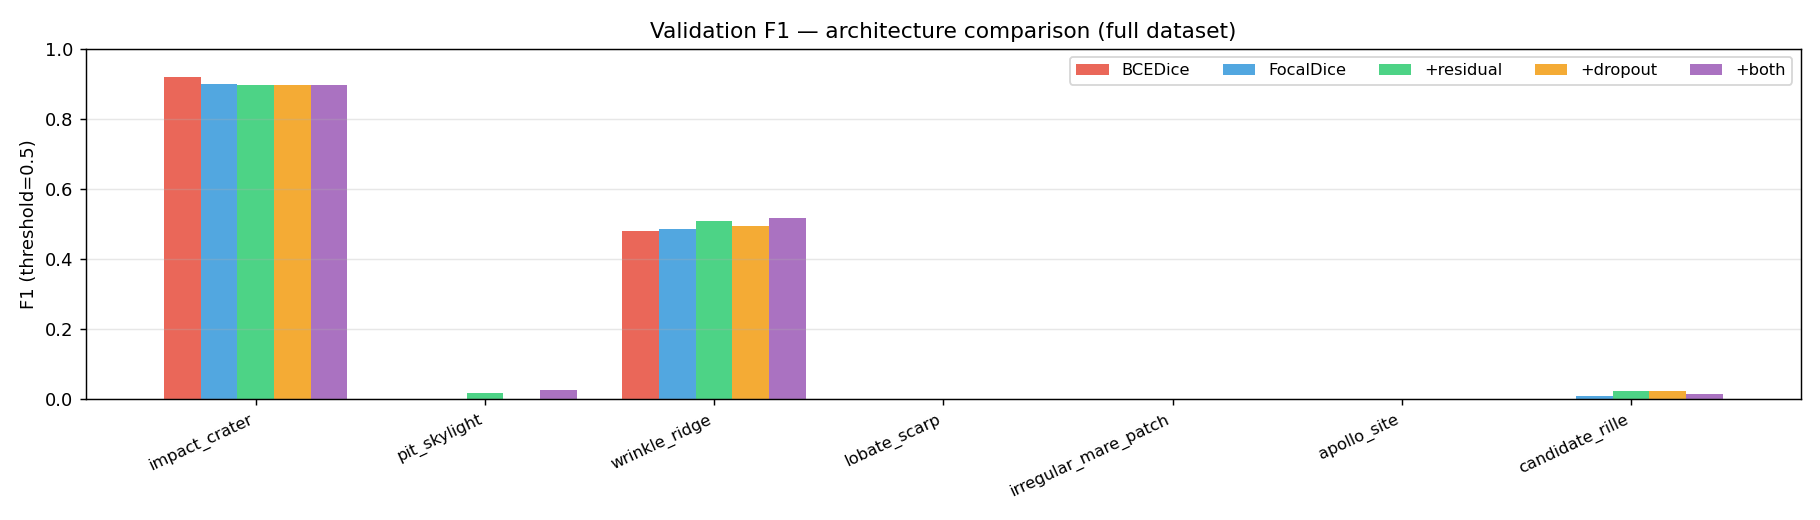
\includegraphics[width=\textwidth]{figures/MR/cloudveneto_arch_val_f1.png}
    \caption{Validation F1}
\end{subfigure}
\hfill
\begin{subfigure}[b]{0.32\textwidth}
    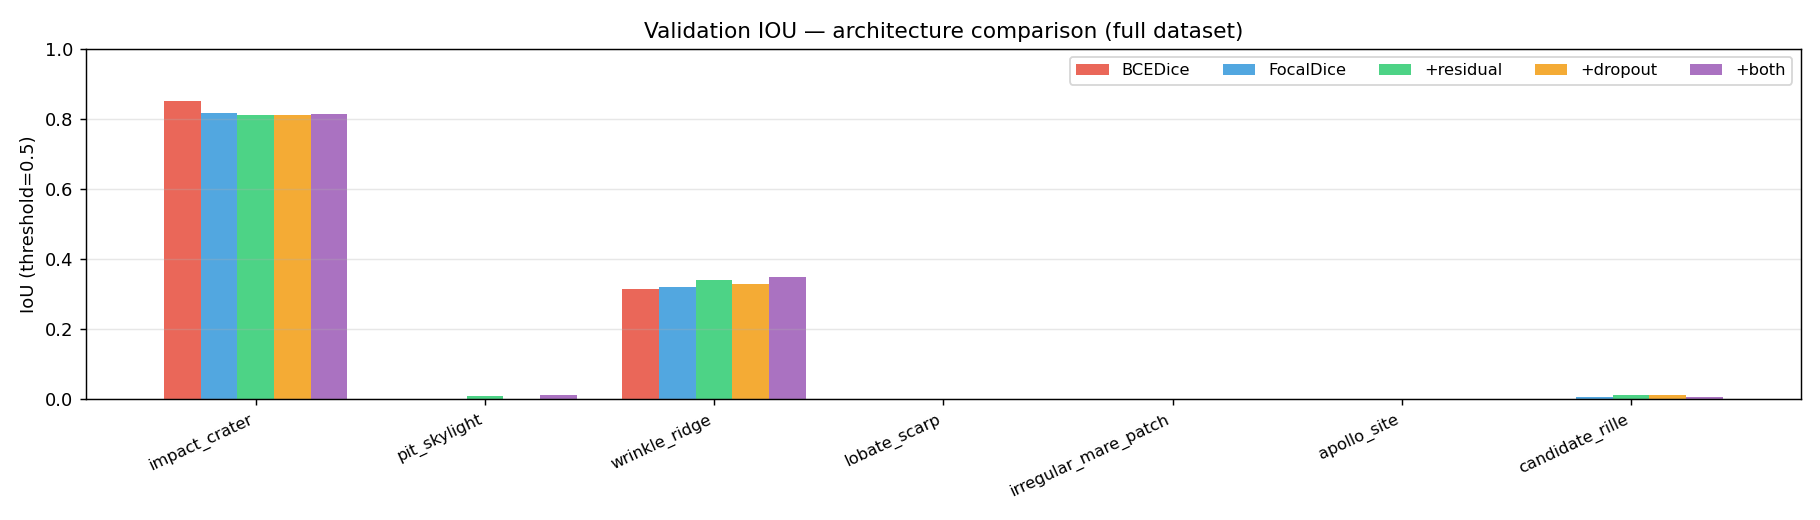
\includegraphics[width=\textwidth]{figures/MR/cloudveneto_arch_val_iou.png}
    \caption{Validation IoU}
\end{subfigure}
\hfill
\begin{subfigure}[b]{0.32\textwidth}
    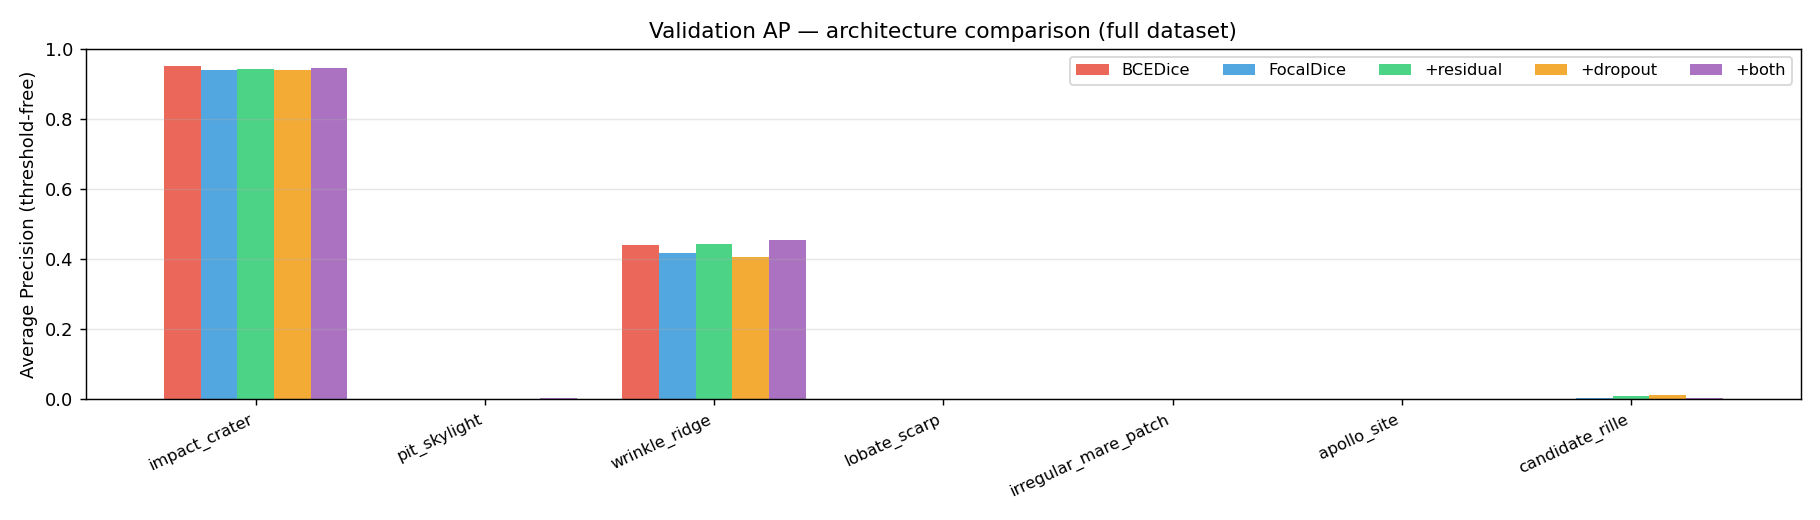
\includegraphics[width=\textwidth]{figures/MR/cloudveneto_arch_val_ap.png}
    \caption{Validation AP}
\end{subfigure}
\caption{Per-class validation metrics across training epochs for the five architecture configurations (full T4 run, 30 epochs). \textbf{+both} (residual + dropout + FocalDice) achieves the highest aggregate performance on all three metrics.}
\label{fig:arch_metrics}
\end{figure}

\paragraph{Key findings.}
Residual shortcuts consistently improve over the plain DoubleConv baseline on aggregate F1, IoU, and AP (+residual vs FocalDice: $+0.0071$ mean F1, $+0.0050$ mean AP). Dropout alone does not help — it degrades both mean AP and ridge AP relative to plain FocalDice, likely because sparse labels already act as a strong regulariser. The combination \textbf{+both} achieves the best mean F1 (0.2076), best mean IoU (0.1688), and best mean AP (0.2004), as well as the highest ridge AP (0.453). Impact-crater AP is uniformly high (0.939–0.951) across all configurations, but given the 0.821 prevalence baseline (Table~\ref{tab:prevalence}) this represents only a modest lift over chance; the architecture choice matters primarily for rare and structurally subtle classes such as ridges, where AP~0.44--0.45 is ${\sim}70\times$ the 0.0064 chance level.

% -----------------------------------------------------------------------------
\subsection{Study 2 — Network Width}
\label{sec:mr_width}

Using the best architecture from Study~1 (\textbf{+both}: FocalDice + residual + dropout=0.3), we sweep the base width $w \in \{16, 32, 64\}$, corresponding to 505K, 2.0M, and 8.0M parameters respectively.

\begin{table}[h]
\centering
\caption{Base-width sweep (FocalDice + residual + dropout=0.3, full T4 run, 30 epochs).}
\label{tab:bw_comparison}
\begin{tabular}{lrrrrrr}
\toprule
Config & Params & Epoch (s) & Mean F1 & Mean IoU & Mean AP & Ridge AP \\
\midrule
small ($w=16$)   &    505{,}095 &  139 & 0.2031 & 0.1665 & 0.2003 & 0.451 \\
default ($w=32$) & 2{,}014{,}727 &  258 & 0.2093 & 0.1704 & 0.2010 & 0.456 \\
wide ($w=64$)    & 8{,}047{,}623 &  582 & \textbf{0.2153} & \textbf{0.1733} & \textbf{0.2016} & 0.445 \\
\bottomrule
\end{tabular}
\end{table}

\begin{figure}[h]
\centering
\begin{subfigure}[b]{0.32\textwidth}
    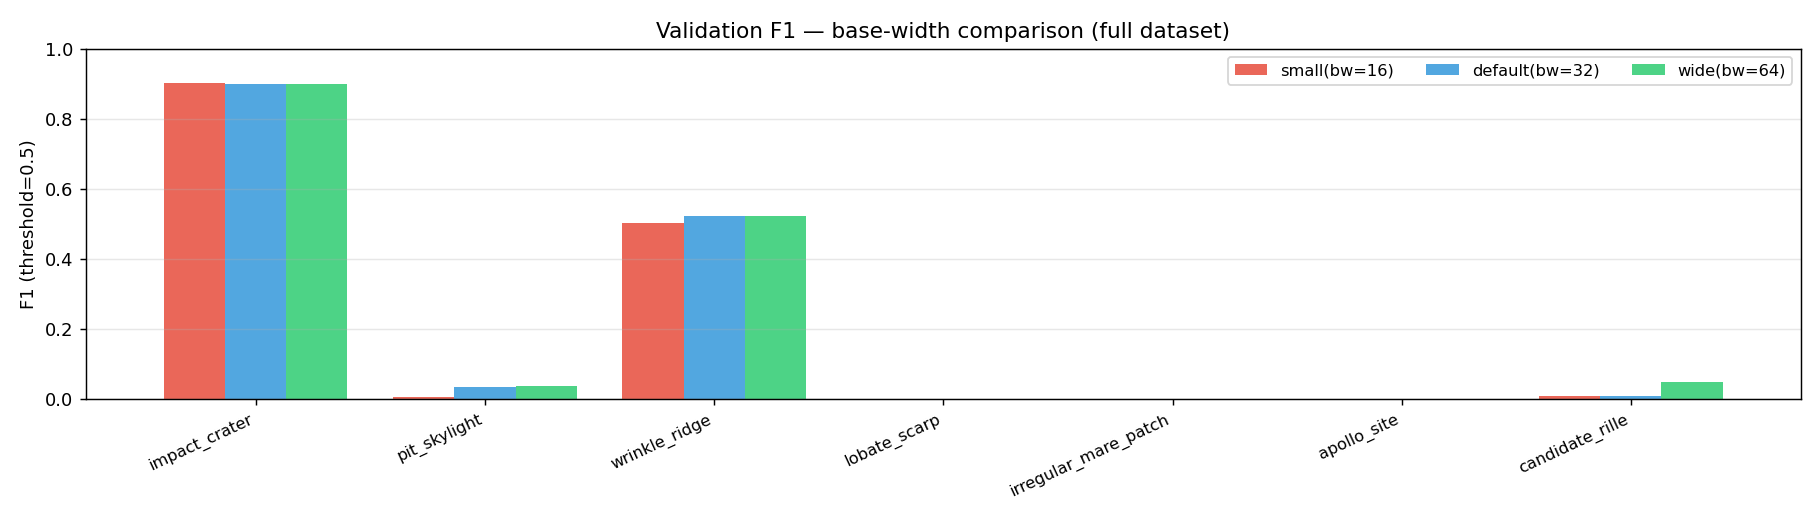
\includegraphics[width=\textwidth]{figures/MR/cloudveneto_bw_val_f1.png}
    \caption{Validation F1}
\end{subfigure}
\hfill
\begin{subfigure}[b]{0.32\textwidth}
    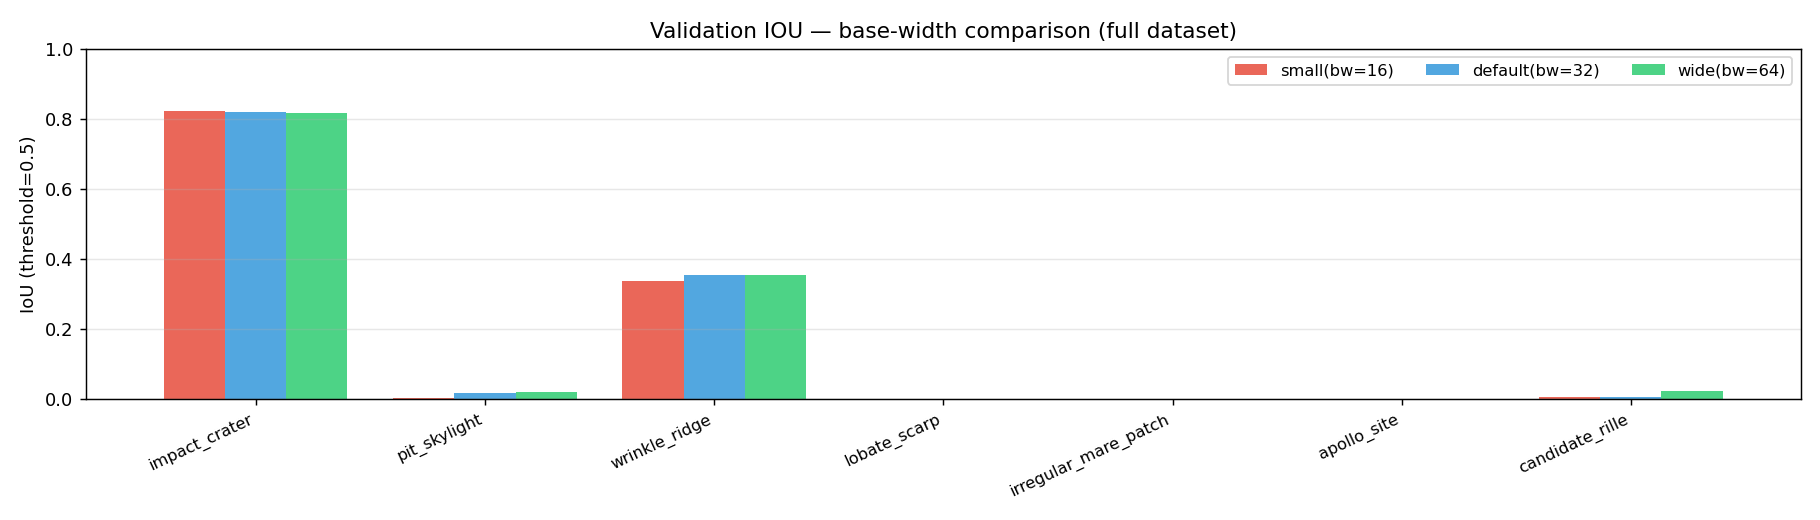
\includegraphics[width=\textwidth]{figures/MR/cloudveneto_bw_val_iou.png}
    \caption{Validation IoU}
\end{subfigure}
\hfill
\begin{subfigure}[b]{0.32\textwidth}
    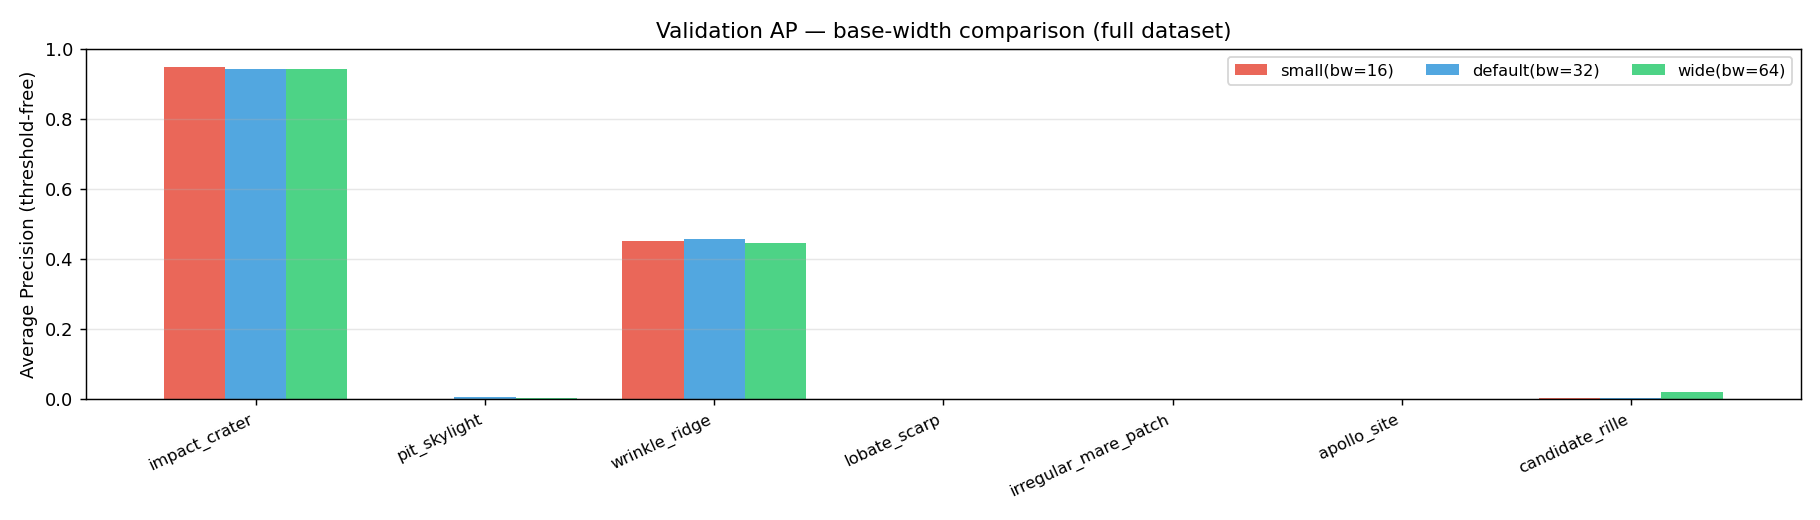
\includegraphics[width=\textwidth]{figures/MR/cloudveneto_bw_val_ap.png}
    \caption{Validation AP}
\end{subfigure}
\caption{Validation metrics for three network widths (full T4 run, 30 epochs). Wider networks achieve marginally higher scores but exhibit severely diminishing returns in terms of parameters and training time.}
\label{fig:bw_metrics}
\end{figure}

\paragraph{Key findings.}
The wide model ($w=64$) achieves the best mean AP (0.2016) and mean F1 (0.2153), but the improvement over the default ($w=32$) is marginal: $+0.0006$ mean AP, $+0.006$ mean F1, at the cost of a 4$\times$ parameter increase and a ${\sim}2.3\times$ increase in training time per epoch (258 s $\to$ 582 s). Strikingly, the small model ($w=16$) with only 505K parameters achieves a mean AP of 0.2003 — within 0.001 of the 8M-parameter wide model — making it the most parameter-efficient option. For deployment on resource-constrained hardware the small model offers the best trade-off.

% -----------------------------------------------------------------------------
\subsection{Study 3 — Data Augmentation}
\label{sec:mr_augmentation}

Using \textbf{+both} at $w=32$, we isolate the effect of geometric augmentation. The augmented pipeline applies random horizontal and vertical flips and 90°/180°/270° rotations to training tiles. No augmentation is applied to validation.

\begin{table}[h]
\centering
\caption{Augmentation study (FocalDice + residual + dropout=0.3, $w=32$, full T4 run, 30 epochs). Crater AP is given for reference; Ridge AP highlights the most affected rare class.}
\label{tab:aug_comparison}
\begin{tabular}{lrrrrrr}
\toprule
Config & Final loss & Mean F1 & Mean IoU & Mean AP & Crater AP & Ridge AP \\
\midrule
\textbf{no augmentation} & \textbf{3.698} & \textbf{0.2986} & \textbf{0.2289} & \textbf{0.2647} & \textbf{0.947} & \textbf{0.558} \\
+augmentation            &        3.863  &        0.2124  &        0.1724  &        0.2027  &        0.942  &        0.457  \\
\bottomrule
\end{tabular}
\end{table}

\begin{figure}[h]
\centering
\begin{subfigure}[b]{0.32\textwidth}
    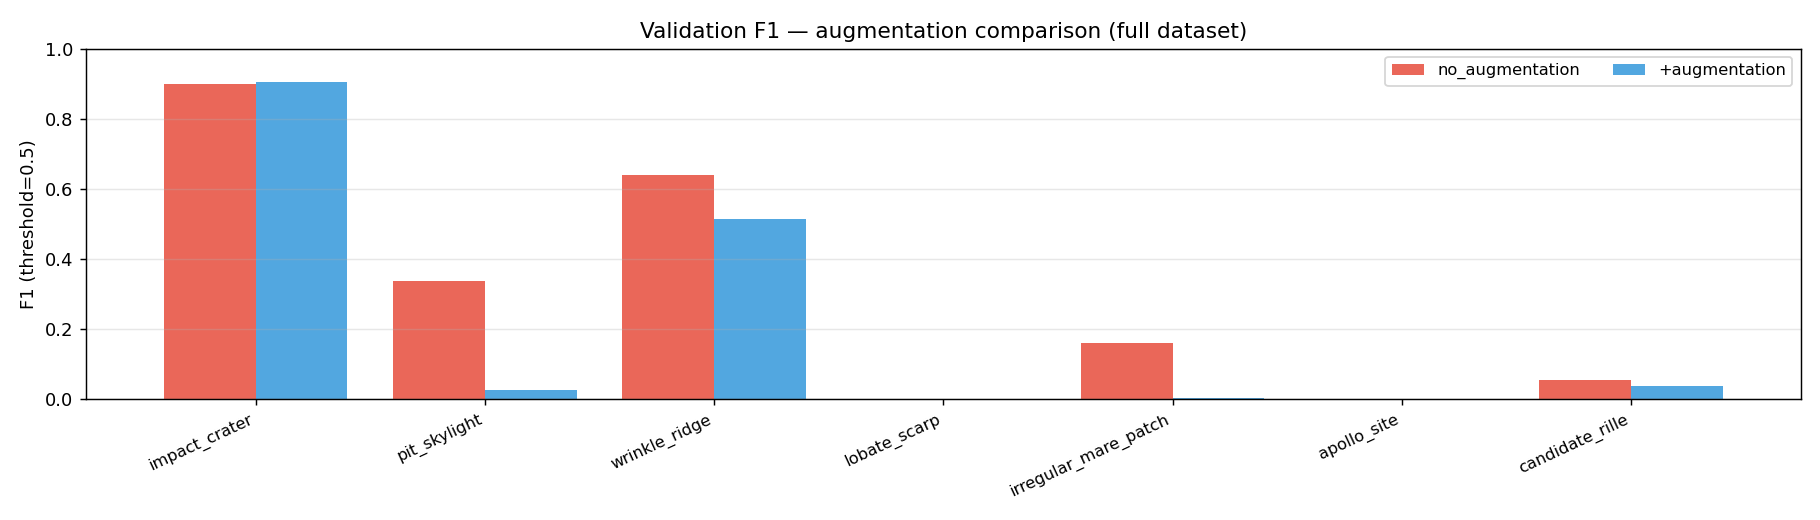
\includegraphics[width=\textwidth]{figures/MR/cloudveneto_aug_val_f1.png}
    \caption{Validation F1}
\end{subfigure}
\hfill
\begin{subfigure}[b]{0.32\textwidth}
    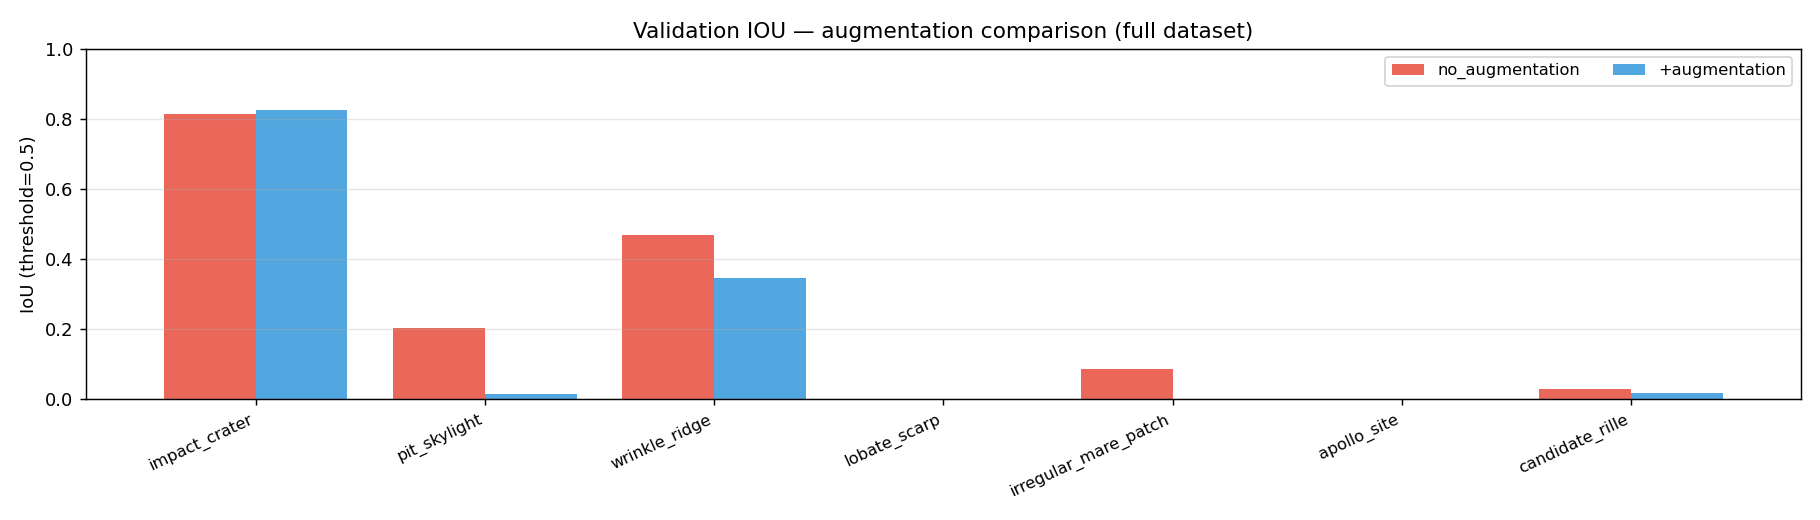
\includegraphics[width=\textwidth]{figures/MR/cloudveneto_aug_val_iou.png}
    \caption{Validation IoU}
\end{subfigure}
\hfill
\begin{subfigure}[b]{0.32\textwidth}
    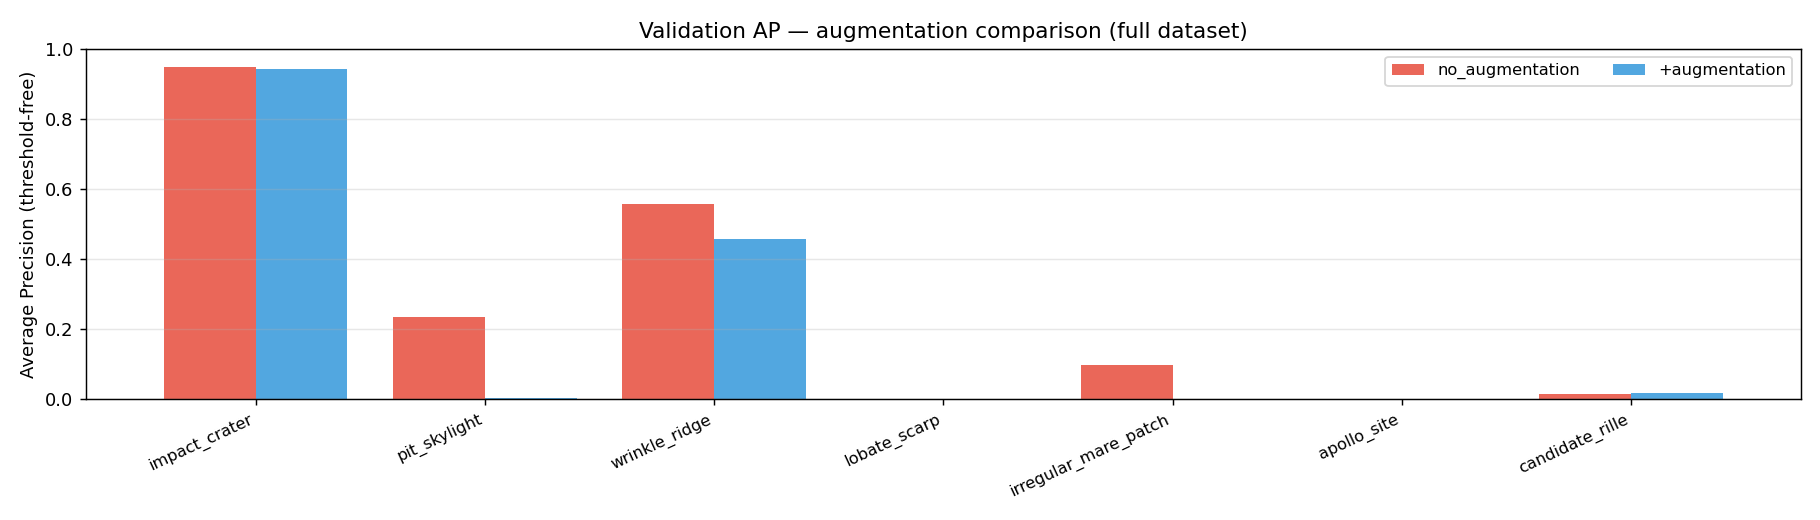
\includegraphics[width=\textwidth]{figures/MR/cloudveneto_aug_val_ap.png}
    \caption{Validation AP}
\end{subfigure}
\caption{Validation metrics with and without geometric augmentation (full T4 run, 30 epochs). No augmentation outperforms the augmented training on all metrics.}
\label{fig:aug_metrics}
\end{figure}

\paragraph{Key findings.}
This is the most striking result of the ablation campaign. Training without augmentation produces a model that is dramatically better on every metric: mean F1 improves by 0.086 (40\% relative), mean AP improves by 0.062 (31\% relative), and ridge AP improves from 0.457 to 0.558 (22\% relative).

Two effects plausibly combine to produce this result, and the present experiment cannot fully separate them.

First, a \emph{geological} effect: the Marius Hills region has a strong directional bias — wrinkle ridges run predominantly in a narrow range of orientations dictated by the regional stress field, and rilles follow the same orientation. Moreover, the Sun azimuth is consistent within the WAC mosaic, so flips and $90°$ rotations also produce illumination directions that never occur in the data. Applying such transforms presents the model with feature orientations and shading that are physically absent in the training region, injecting false diversity. Generic augmentation implicitly assumes that the transformed inputs remain representative of the target distribution~\cite{shorten2019augmentation}, an assumption violated here — the course material itself cautions against ``arbitrary rotations if illumination direction carries physical meaning''~\cite{zingales2026lecture}. Impact craters, being rotationally symmetric, are unaffected, which explains why crater AP is nearly identical in both conditions (0.947 vs 0.942).

Second, a \emph{methodological} confound: as noted in Sec.~\ref{sec:mr_dataset}, the random tile split leaks overlapping pixels into validation. A model trained without augmentation is freer to memorise tile appearance and is rewarded for it on a leaky split, while augmentation suppresses exactly this memorisation. Part of the measured gap could therefore be an artefact of the split rather than a property of the data. To separate the two effects, the comparison was re-run under the leakage-free spatial block split.

\paragraph{Leakage-free re-run.}
The augmentation pair was re-trained with \texttt{spatial\_train\_val\_split}: both arms share an identical pixel-disjoint split, the same initialisation seed, and the same cosine schedule, so the \emph{only} difference between them is augmentation. The re-run used a scaled paired protocol on local hardware (10{,}000 tiles, 30 epochs; a paired comparison remains internally valid at reduced scale), with a smaller 6{,}000-tile/15-epoch run giving consistent results. Table~\ref{tab:spatial_rerun} and Figure~\ref{fig:spatial_rerun} report the outcome.

\begin{table}[h]
\centering
\caption{Augmentation ablation under the leakage-free spatial split (10{,}000 tiles, 30 epochs, paired arms). \texttt{candidate\_rille} has zero positive pixels in the spatial validation set and is excluded from the macro averages (reported as NaN with zero support).}
\label{tab:spatial_rerun}
\begin{tabular}{lrrrr}
\toprule
Config & Mean F1 & Mean AP & Ridge F1 & Ridge AP \\
\midrule
\textbf{no augmentation} & \textbf{0.2294} & \textbf{0.2239} & \textbf{0.4586} & \textbf{0.3847} \\
+augmentation            &        0.2208  &        0.2096  &        0.3970  &        0.3060  \\
\bottomrule
\end{tabular}
\end{table}

\begin{figure}[h]
\centering
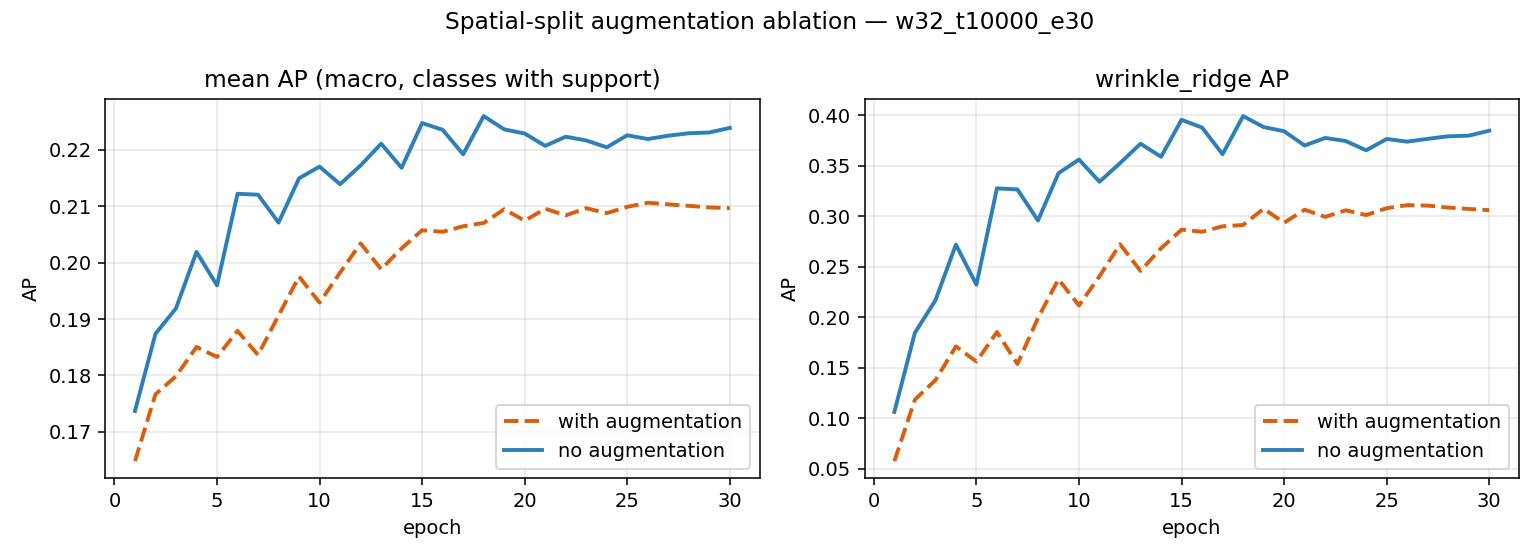
\includegraphics[width=\textwidth]{figures/MR/spatial_w32_t10000_e30_val_ap.png}
\caption{Validation AP across training epochs under the spatial split (macro mean over classes with support, left; \texttt{wrinkle\_ridge}, right). The no-augmentation arm dominates at every epoch on both metrics.}
\label{fig:spatial_rerun}
\end{figure}

The re-run \textbf{confirms the conclusion}: training without augmentation remains better, with the no-augmentation arm above the augmented one at every epoch (Fig.~\ref{fig:spatial_rerun}). The decomposition is, however, instructive. Absolute scores are substantially lower than on the leaky split (ridge AP 0.385 vs 0.558), confirming that random-split numbers were inflated by memorisation. The \emph{aggregate} advantage of no-augmentation also narrows (mean AP $+0.014$ here vs $+0.062$ on the leaky split), showing that part of the originally measured gap was indeed a split artefact. But for the direction-sensitive class the gap persists and is large — ridge AP 0.385 vs 0.306, a 26\% relative difference on strictly disjoint validation pixels — which is precisely the signature predicted by the geological explanation: augmentation hurts where orientation and illumination carry physical information. Confirmation at the full 15{,}931-tile T4 protocol remains scheduled, but the conclusion no longer rests on a confounded measurement.

% -----------------------------------------------------------------------------
\subsection{Qualitative Evaluation}
\label{sec:mr_qualitative}

Segmentation metrics alone do not reveal \emph{how} a model fails, so we complement the ablations with a visual comparison on identical validation tiles: raw image, ground truth, predicted probability, and a true-positive/false-positive/false-negative decomposition at threshold $0.5$, for the BCEDice baseline and the definitive model side by side (generated by \texttt{scripts/qualitative\_eval.py}; tiles are the three validation tiles with the largest \texttt{wrinkle\_ridge} ground-truth area).

\begin{figure}[h]
\centering
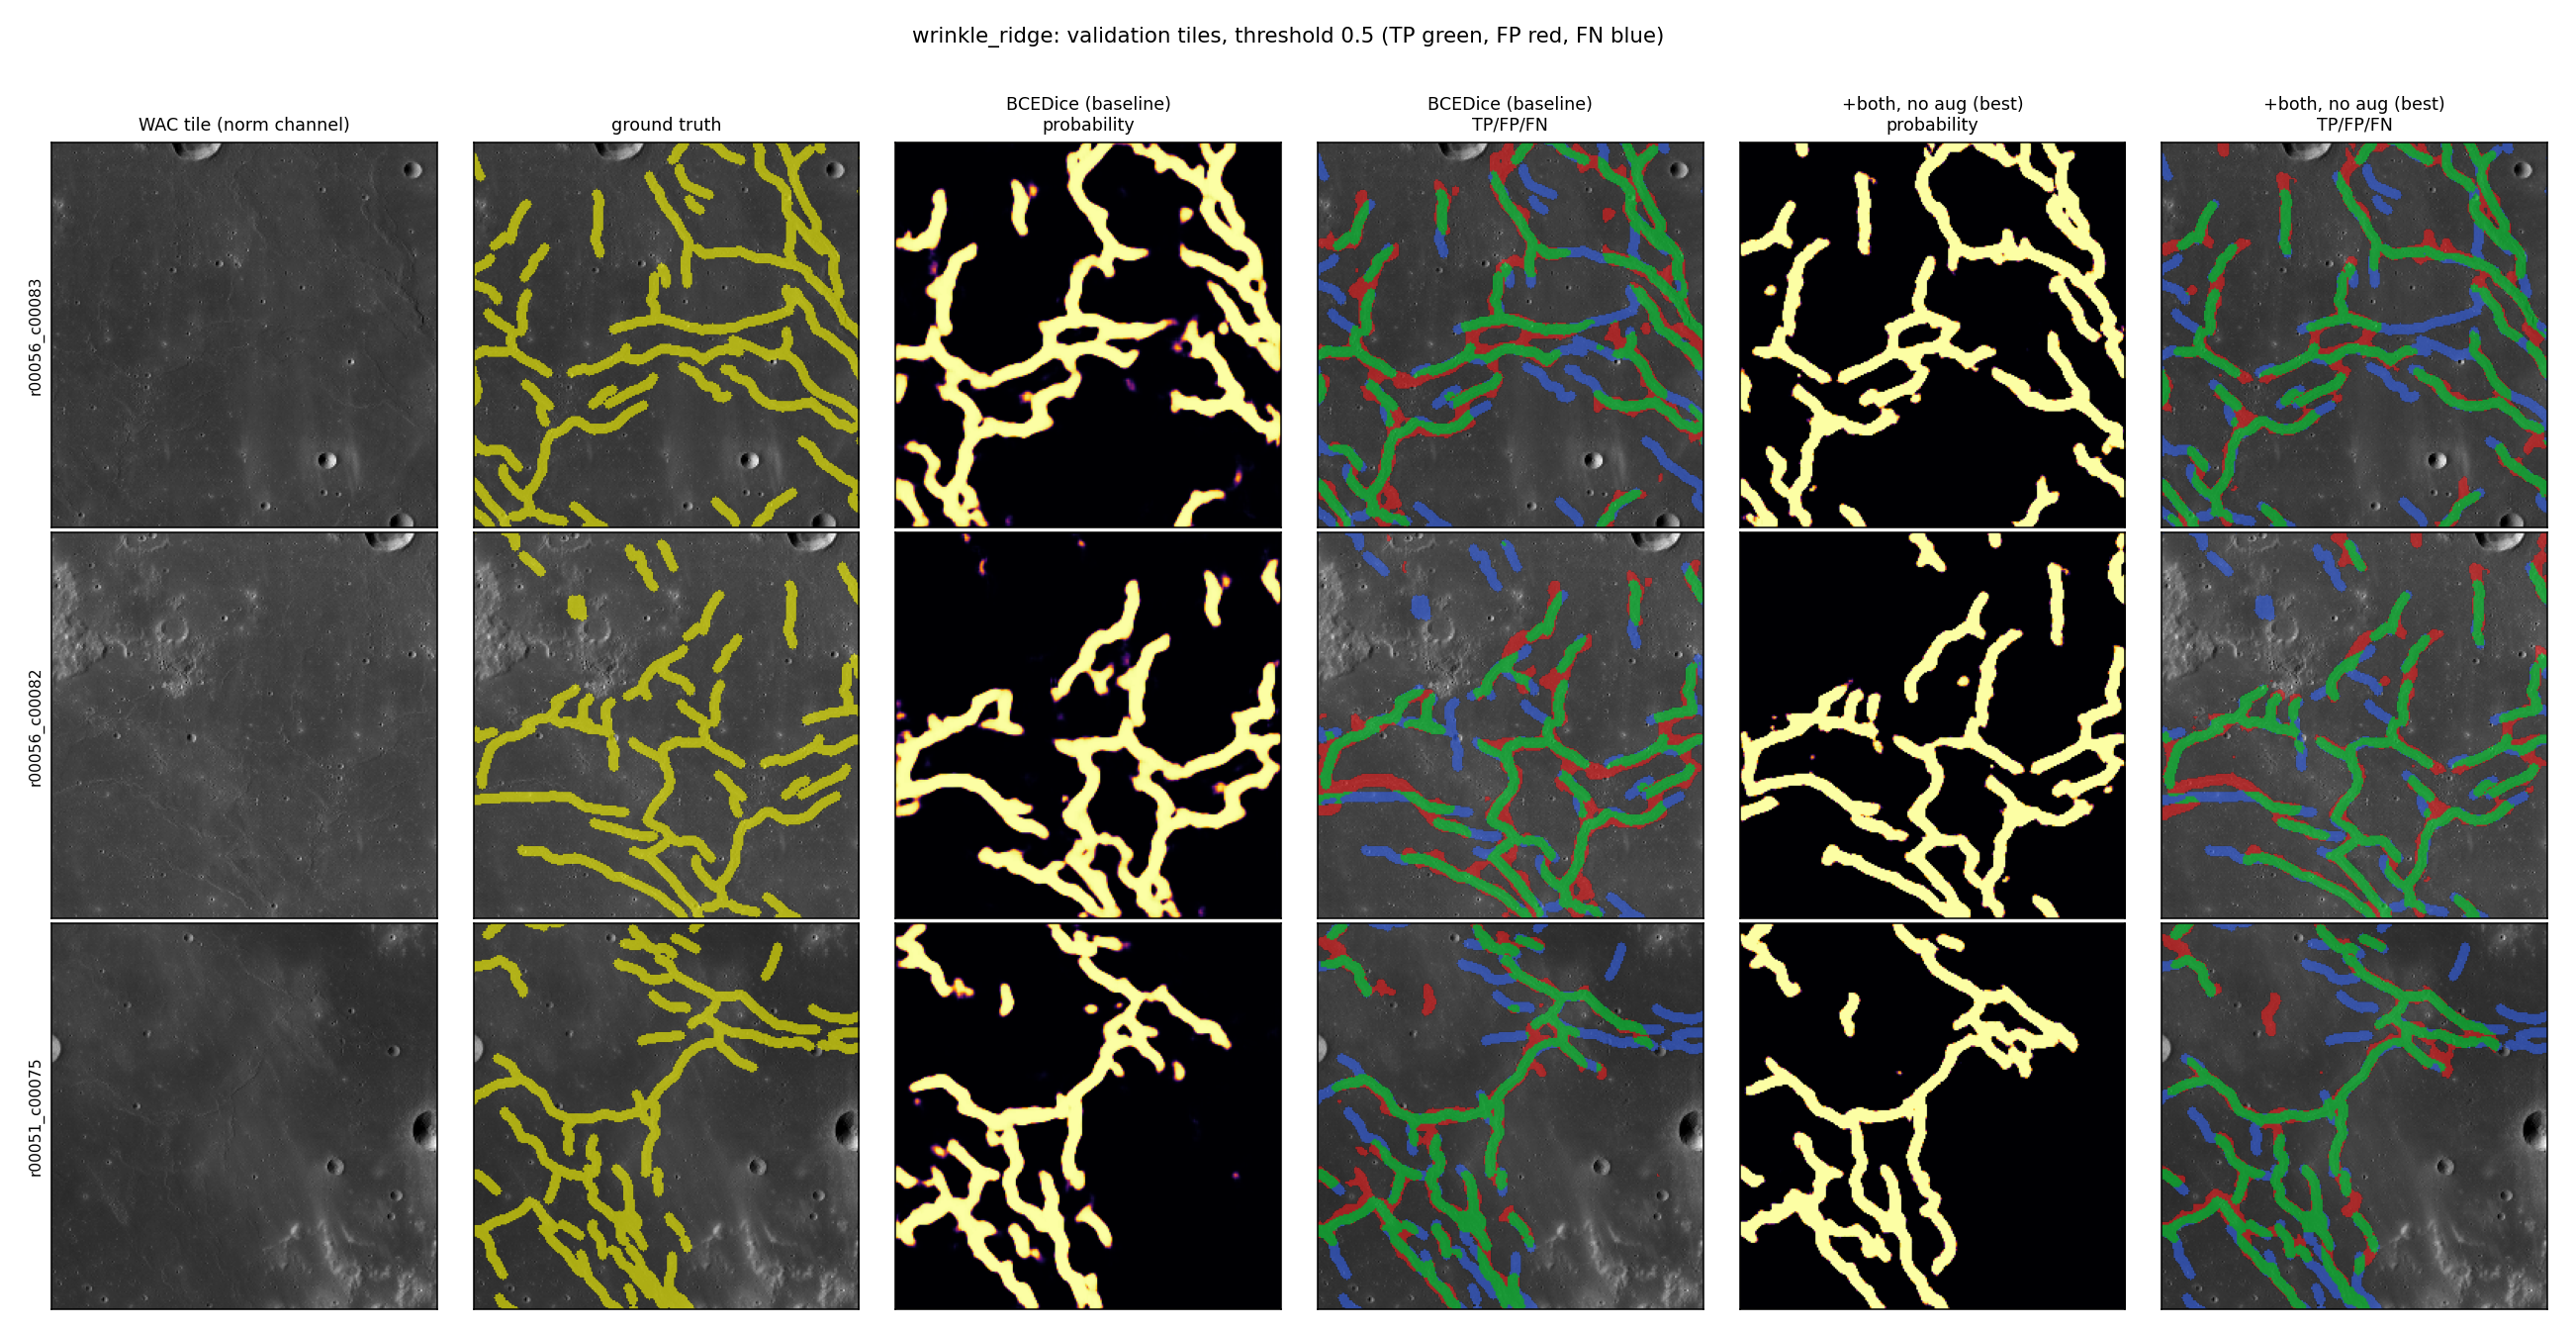
\includegraphics[width=\textwidth]{figures/MR/qualitative_wrinkle_ridge.png}
\caption{Wrinkle-ridge qualitative comparison on three validation tiles (TP green, FP red, FN blue). Both models recover the topology of the ridge network; the definitive model (+both, no augmentation) produces visibly more complete coverage and fewer false positives than the BCEDice baseline. Errors concentrate on thin, low-contrast ridge segments, consistent with the localisation difficulty of linear features.}
\label{fig:qualitative_ridge}
\end{figure}

\begin{figure}[h]
\centering
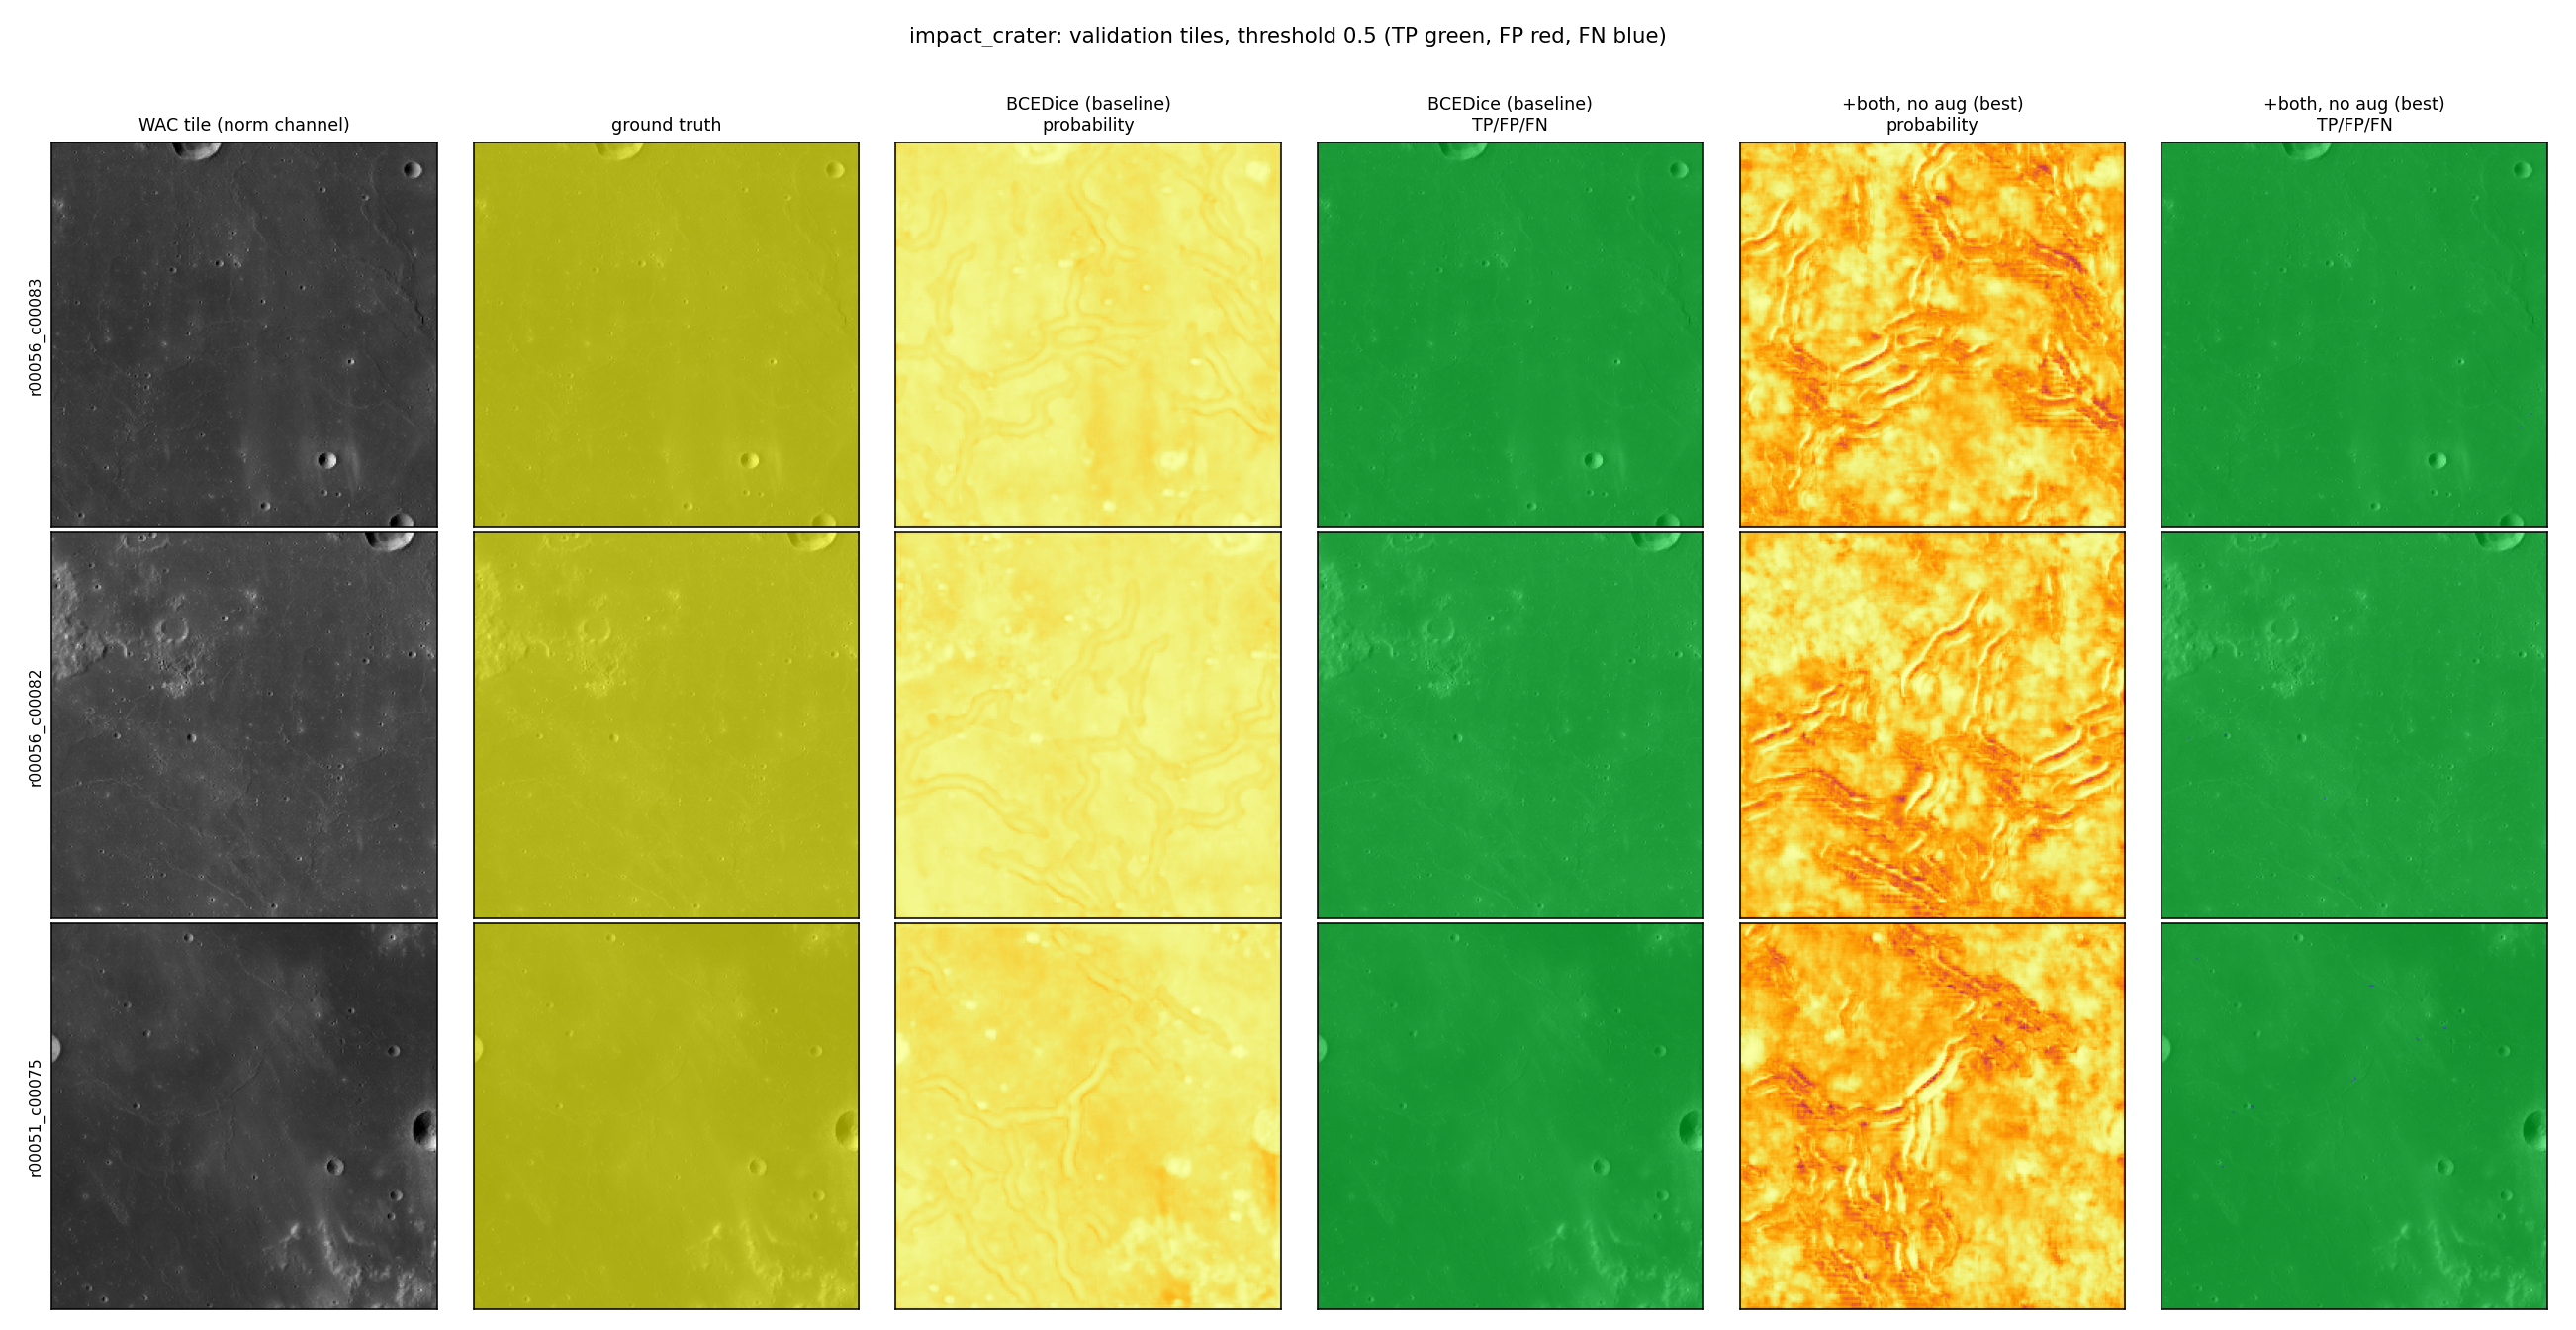
\includegraphics[width=\textwidth]{figures/MR/qualitative_impact_crater.png}
\caption{Impact-crater qualitative comparison on the same tiles. The ground truth covers the \emph{entire} tile (cf.\ the 82\% prevalence and 50.7\% fully-covered tiles of Table~\ref{tab:prevalence}), so a prediction of ``everywhere'' is trivially correct: this figure is direct visual evidence that the crater channel behaves as a near-coverage layer and that crater AP must be read against its 0.821 chance baseline.}
\label{fig:qualitative_crater}
\end{figure}

The ridge comparison shows that the metric gains of the definitive model correspond to a real, visible improvement in completeness of the recovered ridge network. The crater comparison, conversely, makes the saturation argument of Sec.~\ref{sec:mr_dataset} concrete.

% -----------------------------------------------------------------------------
\subsection{South Pole Inference}
\label{sec:mr_south_pole}

The best-performing model weights (\texttt{best\_trained.pth}) were applied to the lunar south pole to demonstrate transfer beyond the training region. The south pole imagery was obtained from the same LRO WAC source and tiled identically, producing 3{,}639 tiles.

\paragraph{Inference pipeline.}
Each tile is preprocessed with the same CLAHE + Sobel three-channel pipeline. A sliding-window predictor runs the model tile by tile, saving per-class probability maps as compressed \texttt{.npz} files for downstream aggregation. Probability maps are aggregated over all tiles to compute global statistics.

\paragraph{Per-class results.}
Table~\ref{tab:south_pole_stats} reports the aggregated statistics over the 3{,}639 south pole tiles.

\begin{table}[h]
\centering
\caption{South pole inference results (3{,}639 tiles). Avg.\ Max.\ Prob.\ is the mean, over tiles, of the maximum predicted probability for each class. Global Max is the highest probability observed in any single tile. A high avg.\ max but low global max indicates diffuse, uncertain detections; a high global max but low avg.\ max indicates rare but confident detections.}
\label{tab:south_pole_stats}
\begin{tabular}{lrrr}
\toprule
Class & Avg.\ Max.\ Prob. & Global Max & Status \\
\midrule
\texttt{impact\_crater}       & 0.863 & 1.000 & \checkmark\ detected \\
\texttt{lobate\_scarp}        & 0.060 & 0.303 & weak \\
\texttt{pit\_skylight}        & 0.051 & 0.202 & weak \\
\texttt{irregular\_mare\_patch} & 0.040 & 0.215 & weak \\
\texttt{apollo\_site}         & 0.040 & 0.183 & weak \\
\texttt{candidate\_rille}     & 0.006 & 0.480 & sparse \\
\texttt{wrinkle\_ridge}       & 0.001 & 1.000 & sparse \\
\bottomrule
\end{tabular}
\end{table}

\begin{figure}[h]
\centering
\begin{subfigure}[b]{0.48\textwidth}
    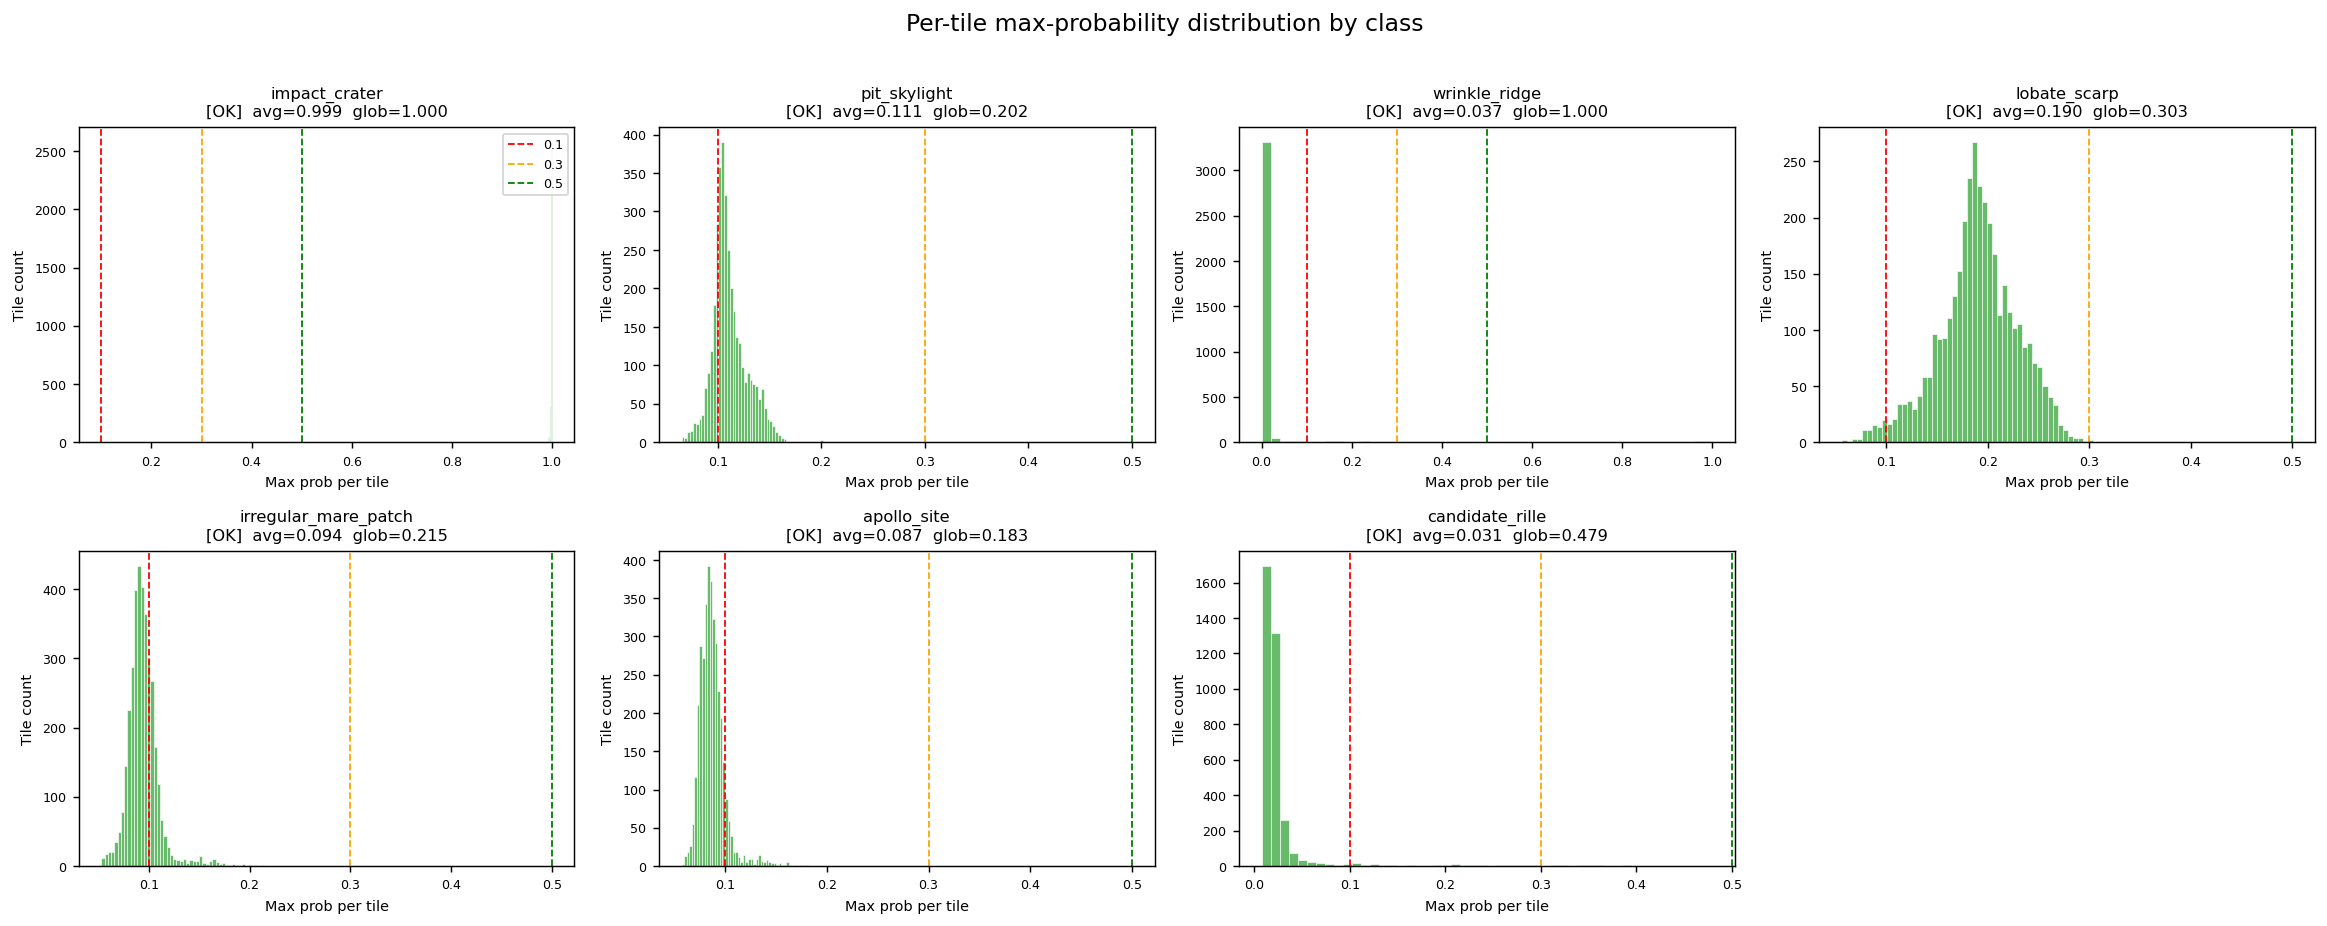
\includegraphics[width=\textwidth]{figures/MR/diagnostics_distributions.png}
    \caption{Per-tile max-probability distributions.}
\end{subfigure}
\hfill
\begin{subfigure}[b]{0.48\textwidth}
    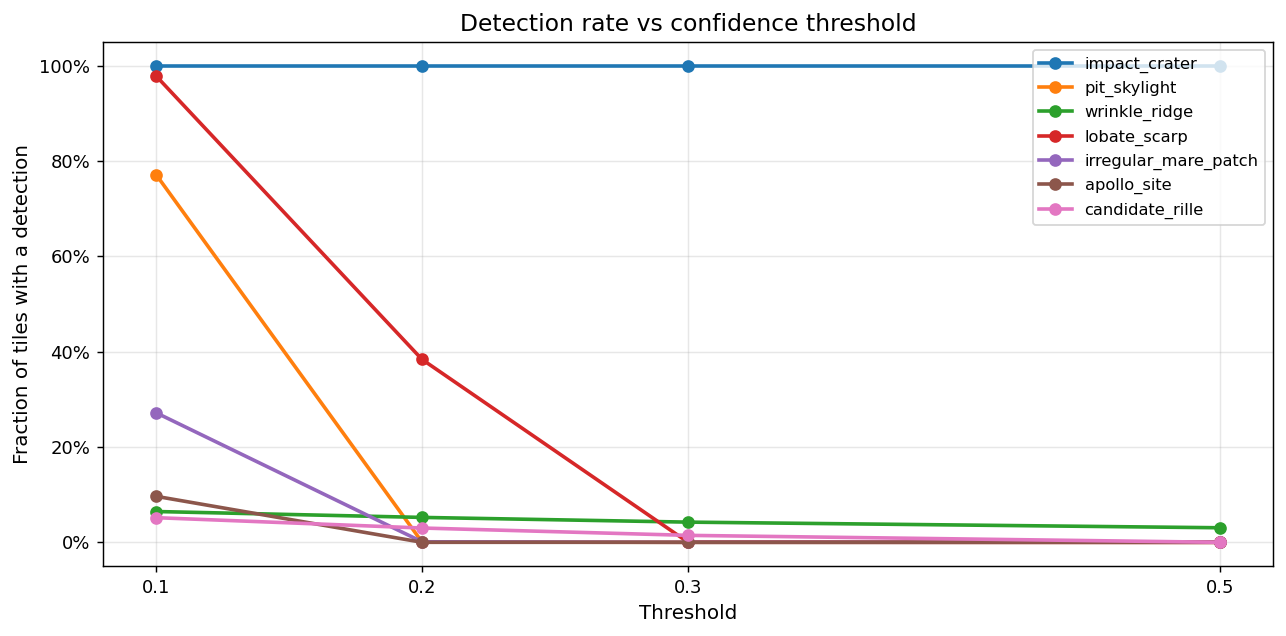
\includegraphics[width=\textwidth]{figures/MR/diagnostics_detection_rates.png}
    \caption{Detection rate vs.\ confidence threshold.}
\end{subfigure}
\caption{South pole inference diagnostics across 3{,}639 tiles. Impact craters are detected with near-certainty across the entire region. All other classes exhibit strongly right-skewed distributions with low average confidence, reflecting both the domain shift from Marius Hills and the scarcity of these features at the south pole.}
\label{fig:south_pole_diag}
\end{figure}

\begin{figure}[h]
\centering
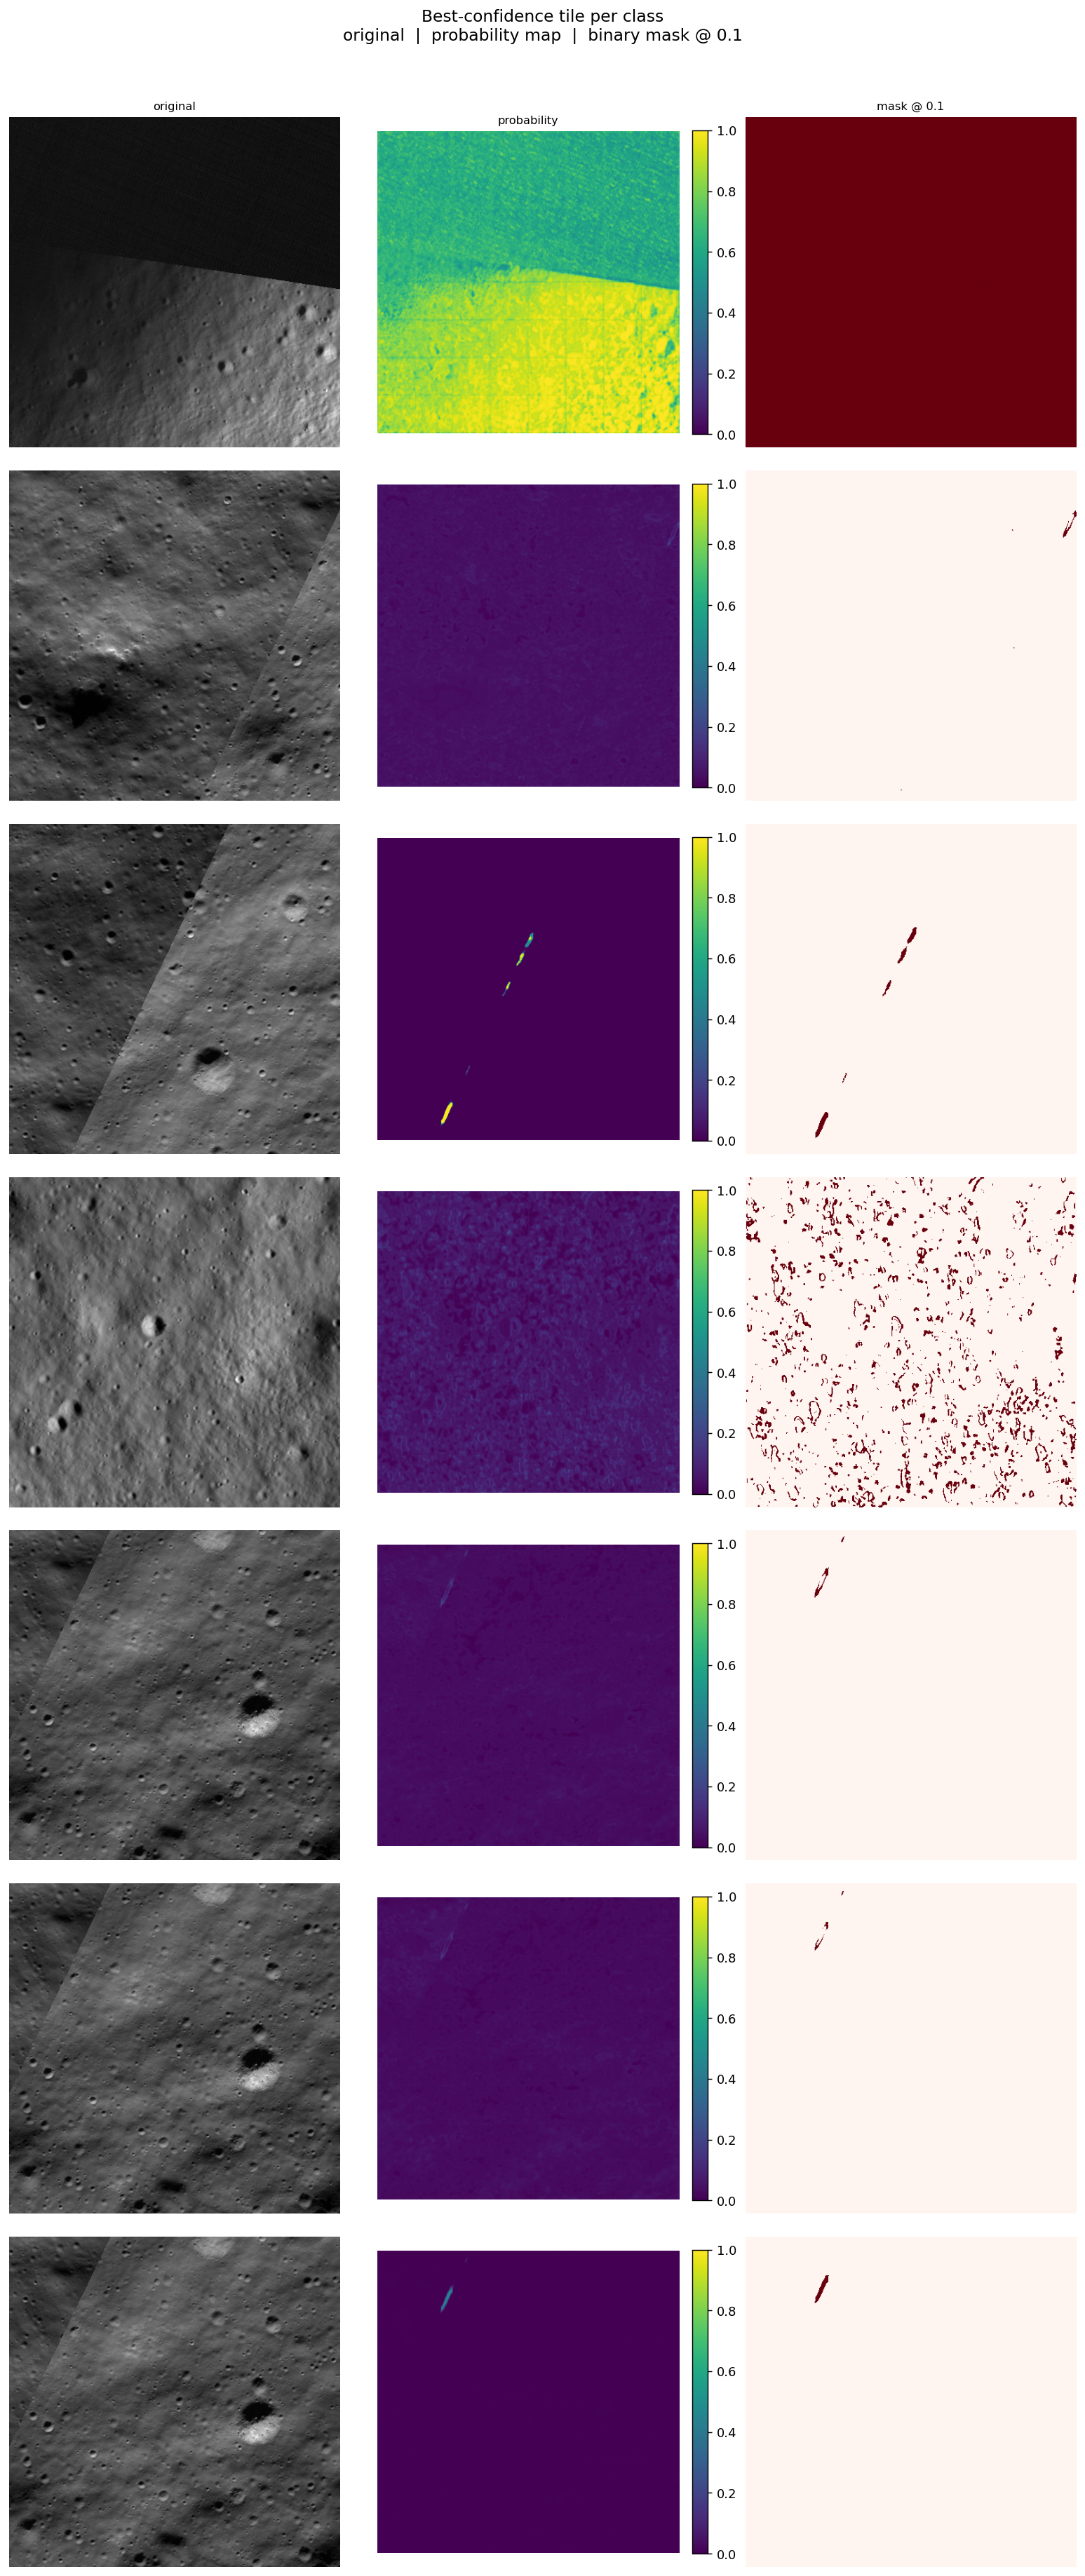
\includegraphics[width=\textwidth, height=0.82\textheight, keepaspectratio]{figures/MR/diagnostics_best_tiles.png}
\caption{Best-detected tile per class on the south pole imagery. Each panel shows the LRO WAC tile overlaid with the predicted probability map for the class with the highest maximum confidence in that tile. Note that overlays use a \emph{relative} threshold (top fraction of each tile's probabilities) so that the most likely candidate pixels are visible even when absolute confidence is low; coloured regions for the weak classes are therefore candidate locations, not confident detections. Impact craters stand out clearly; other classes show localised but low-confidence activations.}
\label{fig:south_pole_best}
\end{figure}

\paragraph{Analysis.}
The model assigns high crater probability across the entire south pole (average max probability 0.863). Given the near-saturated crater layer learned in training (Sec.~\ref{sec:mr_dataset}), this is expected behaviour — the model has learned that almost everywhere is ``crater'' — and should not be over-interpreted as precise crater delineation. Two classes — \texttt{wrinkle\_ridge} and \texttt{candidate\_rille} — show an interesting pattern: very low average-tile probabilities (0.001 and 0.006) but anomalously high global maxima (1.000 and 0.480). This indicates that the model makes rare but high-confidence predictions on a small number of tiles, rather than diffuse low-confidence activations everywhere.

The weak performance on rare classes at the south pole is attributable to two combined factors. First, the south pole is geologically distinct from Marius Hills: it lacks the volcanic structures (skylights, rilles, ridges) that dominate the training distribution, making it an out-of-distribution region for those classes. Second, the extremely low frequency of those classes in the training data means the model has seen very few positive examples even during Marius Hills training. Both issues motivate future work on label-efficient transfer learning and domain adaptation.

% -----------------------------------------------------------------------------
\subsection{Methodological Audit and Reproducibility}
\label{sec:mr_audit}

After the experimental campaign was completed, the entire pipeline — code, data, report claims, and course guidance — was subjected to a systematic audit. Every resulting change is a single, individually justified commit on the \texttt{U-net} branch, indexed in \texttt{Moon-Recognition/IMPROVEMENTS.md}; the executed notebooks were committed \emph{before} any fix, so the provenance of the published numbers is preserved. This section summarises what the audit found and how each finding affects the interpretation of the results — both as a record for the group and because several findings changed the conclusions of this report.

\paragraph{(a) Report--code reconciliation.}
Several statements in an earlier draft did not match the implementation and were corrected against the code as ground truth: the CLAHE parameters (the pipeline uses \texttt{skimage} \texttt{equalize\_adapthist} with clip limit 0.03, not the OpenCV-style values previously quoted), the tiling description (tiles \emph{overlap} by 50\%), the split procedure (random permutation, not sequential), a gradient-clipping claim (clipping was never enabled), and a mis-attributed citation in the augmentation discussion (replaced with the correct survey~\cite{shorten2019augmentation}). The principle applied: any claim an examiner can check against the repository must be checkable.

\paragraph{(b) Train/validation leakage --- discovery and remedy.}
Because adjacent tiles share 50\% of their pixels, the random tile-level split leaks: a direct measurement on the real index showed that \textbf{100\% of the 3{,}186 validation tiles overlap at least one training tile}. This inflates absolute validation scores and specifically confounds the augmentation study, since a non-augmented model is freer to memorise tile appearance and a leaky validation set rewards exactly that memorisation. The remedy, recommended by the course material itself, is a \emph{spatial block split}: contiguous $1024$-px blocks are assigned to validation and every training tile whose footprint intersects a validation tile is discarded ($\texttt{data/splits.py}$; on the real index: 11{,}289 train / 3{,}248 validation tiles, 1{,}394 boundary tiles dropped, zero pixel overlap, verified by an independent assertion). The augmentation comparison was re-run under this split as a scaled paired protocol on local hardware (both arms share an identical split, initialisation, and schedule, so the comparison is internally valid); the conclusion was confirmed, with the expected partial decomposition into a leakage artefact and a genuine effect (Sec.~\ref{sec:mr_augmentation}). Full-protocol confirmation on CloudVeneto remains scheduled when GPU instances become available.

\paragraph{(c) Label audit --- channel saturation.}
A full pass over all 15{,}931 tiles produced the per-class prevalences of Table~\ref{tab:prevalence} and the central reinterpretation of this report: the \texttt{impact\_crater} channel covers 82.1\% of all pixels, making it a near-coverage layer whose AP must be read against a 0.821 chance baseline, while \texttt{wrinkle\_ridge} (prevalence $6.4\times10^{-3}$) emerges as the strongest genuine result and the five rarest classes turn out to have essentially no supervision at all. Without this audit, the headline claim of the report would have been the (nearly trivial) crater result.

\paragraph{(d) Qualitative evaluation.}
The course material requires visual evaluation alongside metrics. Figures~\ref{fig:qualitative_ridge} and~\ref{fig:qualitative_crater} (generated by \texttt{scripts/qualitative\_eval.py} from the full-run checkpoints) confirm both audit findings visually: the metric advantage of the definitive model corresponds to a visibly more complete ridge reconstruction, and the crater ground truth fills entire tiles.

\paragraph{(e) Engineering fixes.}
The audit also produced functional fixes, each preserving the published numbers: evaluation memory reduced by ${\sim}12$\,GB with results verified bit-identical; undefined metrics for classes absent from a validation split now reported as NaN with an explicit support count rather than as a spurious 0; checkpoint loading made compatible with PyTorch $\geq 2.6$ and made loud on architecture/checkpoint mismatches (previously a mismatch silently produced random predictions); the sliding-window inference default aligned with the 256-px training context; dead machine-specific paths removed from the data manifest; and the training configuration file synchronised with the protocol actually used for the published runs.

% -----------------------------------------------------------------------------
\subsection{Summary and Conclusions}
\label{sec:mr_conclusions}

Table~\ref{tab:final_summary} collects the final T4 results for the best configuration identified in each study. The definitive model for the project is \textbf{SmallUNet with $w=32$, FocalDice loss, residual shortcuts, bottleneck dropout ($p=0.3$), trained without augmentation for 30 epochs on the full 15{,}931-tile Marius Hills dataset}. Its weights are stored as \texttt{data/MR/weights/best\_trained.pth}.

\begin{table}[h]
\centering
\caption{Best result from each ablation study (full T4 run, 30 epochs).}
\label{tab:final_summary}
\begin{tabular}{llrrrr}
\toprule
Study & Best config & Params & Mean F1 & Mean AP & Ridge AP \\
\midrule
Architecture & +both ($w=32$, augmented) & 2.0M & 0.2076 & 0.2004 & 0.453 \\
Width        & wide ($w=64$, augmented)  & 8.0M & 0.2153 & 0.2016 & 0.445 \\
Augmentation & +both, $w=32$, \textbf{no aug} & 2.0M & \textbf{0.2986} & \textbf{0.2647} & \textbf{0.558} \\
\bottomrule
\end{tabular}
\end{table}

The principal conclusions of this study are:

\begin{enumerate}
    \item \textbf{Residual shortcuts help; dropout alone does not.} Adding residual connections to DoubleConv blocks consistently improves all aggregate metrics. Bottleneck dropout in isolation hurts performance, likely because sparse labels already regularise the network. The combination \textbf{+both} yields the best augmented-training result.

    \item \textbf{Network width exhibits strong diminishing returns.} The small model ($w=16$, 505K parameters) achieves a mean AP within 0.001 of the wide model ($w=64$, 8M parameters) at one-sixth the training time and ${\sim}16\times$ fewer parameters. For resource-constrained inference the small model is recommended.

    \item \textbf{Geometric augmentation is harmful on this dataset — confirmed under a leakage-free split.} Training without flips and rotations outperforms the augmented model on the original random split, and the advantage survives the spatial block split re-run with strictly disjoint validation pixels (ridge AP 0.385 vs 0.306, no-augmentation above at every epoch). The decomposition is informative: part of the aggregate gap on the random split was a leakage artefact, but the direction-sensitive classes retain a large genuine gap, exactly as predicted by the directional bias of the Marius Hills linear features and the fixed illumination geometry. Augmentation strategies must be tailored to the structural properties of the target domain.

    \item \textbf{Crater AP must be read against its prevalence baseline; ridges are the strongest genuine result.} The \texttt{impact\_crater} channel covers 82.1\% of all pixels (half of the tiles are fully positive), so its AP $\approx 0.95$ is only a modest lift over the 0.821 chance level — the channel behaves as a near-coverage layer, and Fig.~\ref{fig:qualitative_crater} shows that predicting ``everywhere'' is trivially correct. By contrast, \texttt{wrinkle\_ridge} has a prevalence of $6.4\times10^{-3}$, so the best ridge AP of 0.558 is ${\sim}90\times$ chance level and corresponds to a visibly accurate reconstruction of the ridge network (Fig.~\ref{fig:qualitative_ridge}). The remaining five classes have prevalences below $1.4\times10^{-4}$ — their near-zero scores reflect the absence of supervision, not a failure of the architecture.

    \item \textbf{South pole transfer is limited by domain shift and label scarcity.} The model accurately maps impact craters but provides only weak signals for rarer geomorphological features. Acquiring labels for even a small number of south-pole-specific tiles, or employing few-shot domain adaptation, is likely necessary for reliable multi-class south-pole mapping.
\end{enumerate}

% Bibliography entries to add to the main .bib file:
% @inproceedings{ronneberger2015unet,
%   title={U-Net: Convolutional Networks for Biomedical Image Segmentation},
%   author={Ronneberger, Olaf and Fischer, Philipp and Brox, Thomas},
%   booktitle={MICCAI},
%   year={2015}
% }
% @inproceedings{lin2017focal,
%   title={Focal Loss for Dense Object Detection},
%   author={Lin, Tsung-Yi and Goyal, Priya and Girshick, Ross and He, Kaiming and Dollár, Piotr},
%   booktitle={ICCV},
%   year={2017}
% }
% @misc{zingales2026lecture,
%   author={Zingales, Tiziano},
%   title={Moon Features Recognition (Lecture 3b)},
%   howpublished={Computational Physics, Physics of Data, University of Padova},
%   year={2026}
% }
% @article{shorten2019augmentation,
%   title={A survey on Image Data Augmentation for Deep Learning},
%   author={Shorten, Connor and Khoshgoftaar, Taghi M.},
%   journal={Journal of Big Data},
%   volume={6},
%   number={1},
%   pages={60},
%   year={2019}
% }
 from the main document.
%
% Required packages (add to main preamble if not already present):
%   \usepackage{graphicx}
%   \usepackage{booktabs}
%   \usepackage{subcaption}
%   \usepackage{amsmath}
%   \usepackage{amssymb}   % \checkmark in the south-pole table
%   \usepackage{hyperref}
%   \graphicspath{{report/}}   % or adjust to where this file lives
% =============================================================================

\section{Lunar Surface Feature Segmentation}
\label{sec:moon_recognition}

\subsection{Motivation and Task Definition}
\label{sec:mr_motivation}

Accurate mapping of lunar surface features is a prerequisite for mission planning, geological analysis, and the identification of scientifically valuable sites such as lava-tube skylights and impact craters. Manual cataloguing of the high-resolution imagery provided by the Lunar Reconnaissance Orbiter (LRO) is time-consuming and inconsistent. This work frames the problem as \textit{multi-label semantic segmentation}: given a grayscale image patch of the lunar surface, predict, at the pixel level, which of seven geomorphological feature classes are present.

The seven target classes are:
\begin{enumerate}
    \item \texttt{impact\_crater} — circular depressions formed by hypervelocity impacts,
    \item \texttt{pit\_skylight} — openings into subsurface lava tubes,
    \item \texttt{wrinkle\_ridge} — compressional tectonic folds in mare basalts,
    \item \texttt{lobate\_scarp} — cliff-like fault scarps formed by global contraction,
    \item \texttt{irregular\_mare\_patch} — inhomogeneous mare volcanic units,
    \item \texttt{apollo\_site} — Apollo mission landing sites,
    \item \texttt{candidate\_rille} — linear depressions of volcanic or tectonic origin.
\end{enumerate}

\noindent
Because multiple classes can coexist in a single pixel (e.g.\ a pit on the rim of a crater), this is posed as independent binary classification per class rather than a single-label softmax problem.

% -----------------------------------------------------------------------------
\subsection{Dataset}
\label{sec:mr_dataset}

\paragraph{Imagery.}
Training data consists of Wide Angle Camera (WAC) grayscale tiles downloaded from the LROC archive, covering the \textit{Marius Hills} volcanic region on the Oceanus Procellarum — a site of particular scientific interest due to its high density of pit skylights, wrinkle ridges, and rilles.

\paragraph{Tiling.}
The raw raster is divided into overlapping training patches using a sliding-window tiler:
\begin{itemize}
    \item Tile size: $256 \times 256$ pixels,
    \item Stride: $128$ pixels (50\% overlap between adjacent tiles),
    \item Tiles with no labelled features are kept with probability $p=0.1$ to maintain background examples,
    \item Total tiles produced: 15{,}931.
\end{itemize}

\paragraph{Labels.}
Ground-truth annotations are sourced from the LROC feature catalogue (shapefiles and CSV), rasterised onto the tile grid as binary masks. To account for the point-like or line-like nature of some classes, morphological dilation is applied per class after rasterisation:
\begin{itemize}
    \item \texttt{pit\_skylight}, \texttt{apollo\_site}, \texttt{irregular\_mare\_patch}: disk kernel of radius 5,
    \item \texttt{wrinkle\_ridge}, \texttt{lobate\_scarp}: disk kernel of radius 3 (linear features),
    \item \texttt{candidate\_rille}: disk kernel of radius 2,
    \item \texttt{impact\_crater}: no dilation (already area features).
\end{itemize}

\paragraph{Train / validation split.}
Tiles are split 80/20 by random permutation with a fixed seed (42), yielding 12{,}745 training tiles and 3{,}186 validation tiles; the same split is reused across all configurations so that comparisons between models are paired.

\paragraph{Label prevalence and channel saturation.}
Table~\ref{tab:prevalence} reports the exact fraction of positive pixels per class, computed over all 15{,}931 tiles. The imbalance is extreme \emph{in both directions}: the \texttt{impact\_crater} channel covers 82.1\% of all pixels — half of the tiles are \emph{entirely} positive — while the five rarest classes have prevalences below $1.4\times10^{-4}$. The crater channel therefore behaves closer to a coverage-like layer than to a sparse target feature, a possibility explicitly flagged in the course material (``do not assume every positive pixel is a target feature without inspecting channels''). This has a direct consequence for interpretation: the Average Precision of an uninformative predictor equals the class prevalence, so per-class AP values must be read against the baselines in Table~\ref{tab:prevalence} rather than against zero.

\begin{table}[h]
\centering
\caption{Per-class positive-pixel prevalence over the full dataset (15{,}931 tiles, $1.04\times10^9$ pixels per channel). The prevalence is also the AP of an uninformative (chance-level) predictor for that class.}
\label{tab:prevalence}
\begin{tabular}{lrr}
\toprule
Class & Prevalence & Tiles fully covered \\
\midrule
\texttt{impact\_crater}        & $8.21\times10^{-1}$ & 50.7\% \\
\texttt{wrinkle\_ridge}        & $6.38\times10^{-3}$ & 0 \\
\texttt{lobate\_scarp}         & $1.34\times10^{-4}$ & 0 \\
\texttt{pit\_skylight}         & $4.2\times10^{-5}$  & 0 \\
\texttt{irregular\_mare\_patch} & $2.0\times10^{-5}$  & 0 \\
\texttt{apollo\_site}          & $1.5\times10^{-5}$  & 0 \\
\texttt{candidate\_rille}      & $1.0\times10^{-5}$  & 0 \\
\bottomrule
\end{tabular}
\end{table}

\paragraph{Limitation: spatial overlap between splits.}
Because adjacent tiles overlap by 50\%, a random tile-level split leaks pixels between the two sets: we measured that \emph{every} validation tile overlaps at least one training tile. Absolute validation scores are therefore optimistic (they partially reward memorisation of seen pixels), although \emph{relative} comparisons between configurations trained and evaluated on the identical split remain informative. A leakage-free \emph{spatial block split} (contiguous $1024$-px blocks assigned to validation, with overlapping boundary tiles discarded from training) has been implemented in \texttt{data/splits.py}; its impact is discussed where relevant, in particular for the augmentation study (Sec.~\ref{sec:mr_augmentation}).

% -----------------------------------------------------------------------------
\subsection{Input Pre-processing Pipeline}
\label{sec:mr_preprocessing}

Each grayscale tile is converted into a three-channel tensor to provide the network with complementary representations of the same image:

\begin{enumerate}
    \item \textbf{Normalised intensity}: min-max normalisation of the raw pixel values to $[0,1]$.
    \item \textbf{CLAHE}: Contrast Limited Adaptive Histogram Equalization (\texttt{skimage.exposure.equalize\_adapthist}, clip limit $0.03$, default kernel of $1/8$ of the image side) to enhance local contrast and make faint features more visible.
    \item \textbf{Sobel edges}: magnitude of the Sobel gradient computed on the normalised tile, highlighting boundaries and ridge-like structures.
\end{enumerate}

\noindent
Because CLAHE is computationally expensive (${\sim}3$ s per tile on CPU), a one-time precomputation step caches all three-channel tensors as compressed \texttt{.npz} files. During training and inference, tiles are loaded from cache, eliminating the CLAHE bottleneck from the data pipeline.

% -----------------------------------------------------------------------------
\subsection{Model Architecture: SmallUNet}
\label{sec:mr_architecture}

The model follows the U-Net encoder-decoder paradigm~\cite{ronneberger2015unet} with modifications designed to reduce parameter count while preserving multi-scale feature reuse.

\paragraph{Encoder.}
Three successive \textit{Down} blocks, each consisting of $2\times 2$ max-pooling followed by a \textit{DoubleConv} block. A DoubleConv block applies two consecutive $3\times 3$ convolution $\to$ BatchNorm $\to$ ReLU operations.

\paragraph{Decoder.}
Three symmetric \textit{Up} blocks, each using transposed convolution for $2\times$ upsampling, concatenation with the corresponding encoder skip connection, and a DoubleConv block. Odd-dimension padding ensures spatial alignment between encoder and decoder feature maps.

\paragraph{Output head.}
A $1\times 1$ convolution maps the final feature map (32 channels) to 7 independent logit channels. Binary sigmoid is applied per channel at inference time to produce class probability maps.

\paragraph{Optional residual shortcuts.}
Each DoubleConv block can optionally include a residual (ResNet-style) shortcut: the block input is added to the post-convolution output before the final ReLU, with a $1\times 1$ projection convolution when channel dimensions differ. This improves gradient flow and slightly increases parameter count.

\paragraph{Bottleneck dropout.}
Spatial Dropout2d can be applied at the bottleneck (deepest encoder level) to regularise the model when training labels are sparse.

The spatial flow of the network with base width $w=32$ and $256\times 256$ input is:

\[
(3,\,256,256)
\xrightarrow{\text{inc}}   (32,\,256,256)
\xrightarrow{\text{down}_1}(64,\,128,128)
\xrightarrow{\text{down}_2}(128,\,64,64)
\xrightarrow{\text{down}_3}(256,\,32,32)
\]
\[
\xrightarrow{\text{up}_1}  (128,\,64,64)
\xrightarrow{\text{up}_2}  (64,\,128,128)
\xrightarrow{\text{up}_3}  (32,\,256,256)
\xrightarrow{\text{out}}   (7,\,256,256)
\]

\noindent
The base width $w$ is configurable; doubling $w$ quadruples the parameter count. The three widths explored in this work are summarised in Table~\ref{tab:bw_params}.

\begin{table}[h]
\centering
\caption{Parameter counts for each base width.}
\label{tab:bw_params}
\begin{tabular}{lrr}
\toprule
Base width $w$ & Channel progression & Parameters \\
\midrule
16 & 16--32--64--128  &    505{,}095 \\
32 & 32--64--128--256 & 2{,}014{,}727 \\
64 & 64--128--256--512 & 8{,}047{,}623 \\
\bottomrule
\end{tabular}
\end{table}

% -----------------------------------------------------------------------------
\subsection{Loss Functions}
\label{sec:mr_loss}

Two composite loss functions are compared.

\paragraph{BCEDiceLoss.}
Binary cross-entropy summed with a soft Dice loss, averaged across classes:
\[
\mathcal{L}_{\text{BCEDice}} = \mathcal{L}_{\text{BCE}} + \mathcal{L}_{\text{Dice}},
\qquad
\mathcal{L}_{\text{Dice}} = 1 - \frac{1}{C}\sum_{c=1}^{C} \frac{2\sum_i p_i^c\, y_i^c + \varepsilon}{\sum_i p_i^c + \sum_i y_i^c + \varepsilon}
\]
where $p_i^c$ is the predicted probability and $y_i^c$ the ground-truth label for pixel $i$ and class $c$, and $\varepsilon=10^{-6}$ ensures numerical stability.

\paragraph{FocalDiceLoss.}
Replaces the BCE term with the binary focal loss~\cite{lin2017focal} to down-weight easy negatives and focus training on hard positives, a natural choice for class-imbalanced segmentation:
\[
\mathcal{L}_{\text{focal}}(p,y) = -\alpha\,y\,(1-p)^\gamma \log p
                                   -(1-\alpha)(1-y)\,p^\gamma \log(1-p)
\]
with $\gamma=2$ and $\alpha=0.25$. The Dice term additionally uses per-class weights $\mathbf{w} = [1.0,\,4.0,\,5.0,\,5.0,\,5.0,\,5.0,\,5.0]$ to penalise misdetection of rare classes more heavily:
\[
\mathcal{L}_{\text{FocalDice}} = \mathcal{L}_{\text{focal}} + \sum_{c=1}^{C} w_c \,\mathcal{L}_{\text{Dice}}^c
\]

% -----------------------------------------------------------------------------
\subsection{Training Protocol}
\label{sec:mr_training}

All definitive experiments were run on a \textbf{NVIDIA Tesla T4} (16 GB VRAM) via the CloudVeneto HPC facility, using the full training dataset of 15{,}931 tiles for 30 epochs. The local MPS (Apple Silicon) runs at 4{,}000 tiles / 20 epochs served as rapid prototyping before the full runs.

\begin{itemize}
    \item Batch size: 16 (T4) / 8 (MPS),
    \item Optimizer: Adam,
    \item Learning rate schedule: cosine annealing, $\eta_{\max}=10^{-3}$, $\eta_{\min}=10^{-5}$, $T_{\max}=30$,
    \item No gradient clipping (the trainer supports it, but it was disabled in all runs: \texttt{clip\_grad\_norm\_} forces a CPU synchronisation per batch on MPS),
    \item Checkpoints saved at end of training for each experimental configuration.
\end{itemize}

\paragraph{Metrics.}
Validation is performed after every epoch. For each class $c$ and a fixed threshold $\tau=0.5$ we compute precision, recall, F1, and Intersection over Union (IoU); for binary pixel masks the F1 score coincides with the Dice coefficient, $2\,\mathrm{TP}/(2\,\mathrm{TP}+\mathrm{FP}+\mathrm{FN})$, so per-class Dice and IoU are both reported. A class with no positive pixels in a given validation split has undefined metrics and is excluded from macro averages (reported as NaN with its support count). Additionally, \textit{Average Precision} (AP) is computed as the area under the precision-recall curve (threshold-free), using \texttt{sklearn.metrics.average\_precision\_score}. Aggregate metrics are macro-averages across the seven classes.

% -----------------------------------------------------------------------------
\subsection{Study 1 — Architecture Ablation}
\label{sec:mr_arch_ablation}

Five configurations are compared in a cumulative fashion, each adding one component to the previous best:

\begin{enumerate}
    \item \textbf{BCEDice}: plain DoubleConv blocks, BCEDiceLoss — the reference baseline.
    \item \textbf{FocalDice}: same architecture, FocalDiceLoss with class weights.
    \item \textbf{+residual}: FocalDice + residual shortcuts inside DoubleConv blocks.
    \item \textbf{+dropout}: FocalDice + bottleneck Dropout2d($p=0.3$).
    \item \textbf{+both}: FocalDice + residual + dropout.
\end{enumerate}

Table~\ref{tab:arch_comparison} reports the full-run results (15{,}931 tiles, 30 epochs, T4).
Figure~\ref{fig:arch_metrics} shows the per-class validation curves.

\begin{table}[h]
\centering
\caption{Architecture ablation on the full dataset (Tesla T4, 30 epochs). Metrics are macro-averaged across the seven classes. Crater AP and Ridge AP are single-class AP values for \texttt{impact\_crater} and \texttt{wrinkle\_ridge}, which span the performance range.}
\label{tab:arch_comparison}
\begin{tabular}{lrrrrrrr}
\toprule
Config & Params & Epoch (s) & Final loss & Mean F1 & Mean IoU & Mean AP & Ridge AP \\
\midrule
BCEDice    & 1{,}927{,}207 & 208 & 0.876 & 0.1998 & 0.1666 & 0.1989 & 0.440 \\
FocalDice  & 1{,}927{,}207 & 214 & 3.893 & 0.1994 & 0.1632 & 0.1945 & 0.417 \\
+residual  & 2{,}014{,}727 & 257 & 3.873 & 0.2065 & 0.1675 & 0.1995 & 0.443 \\
+dropout   & 1{,}927{,}207 & 215 & 3.894 & 0.2018 & 0.1643 & 0.1938 & 0.405 \\
\textbf{+both} & \textbf{2{,}014{,}727} & 258 & \textbf{3.863} & \textbf{0.2076} & \textbf{0.1688} & \textbf{0.2004} & \textbf{0.453} \\
\bottomrule
\end{tabular}
\end{table}

\begin{figure}[h]
\centering
\begin{subfigure}[b]{0.32\textwidth}
    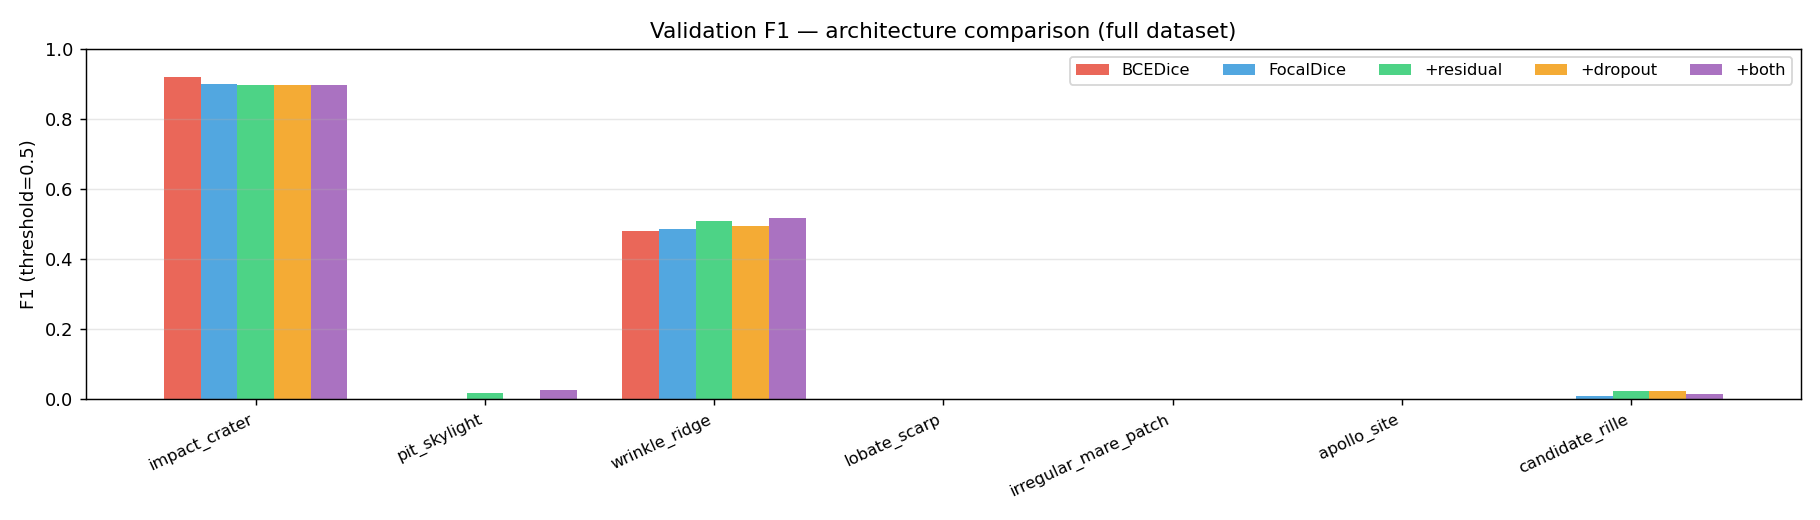
\includegraphics[width=\textwidth]{figures/MR/cloudveneto_arch_val_f1.png}
    \caption{Validation F1}
\end{subfigure}
\hfill
\begin{subfigure}[b]{0.32\textwidth}
    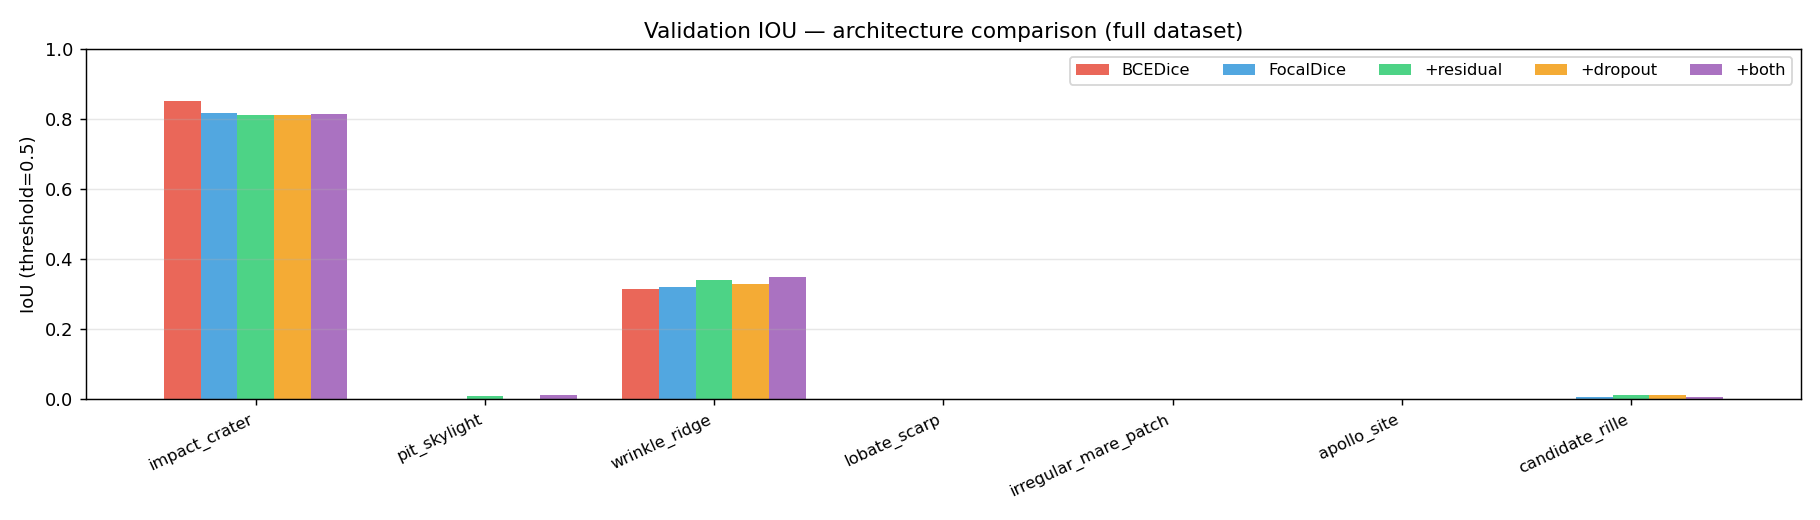
\includegraphics[width=\textwidth]{figures/MR/cloudveneto_arch_val_iou.png}
    \caption{Validation IoU}
\end{subfigure}
\hfill
\begin{subfigure}[b]{0.32\textwidth}
    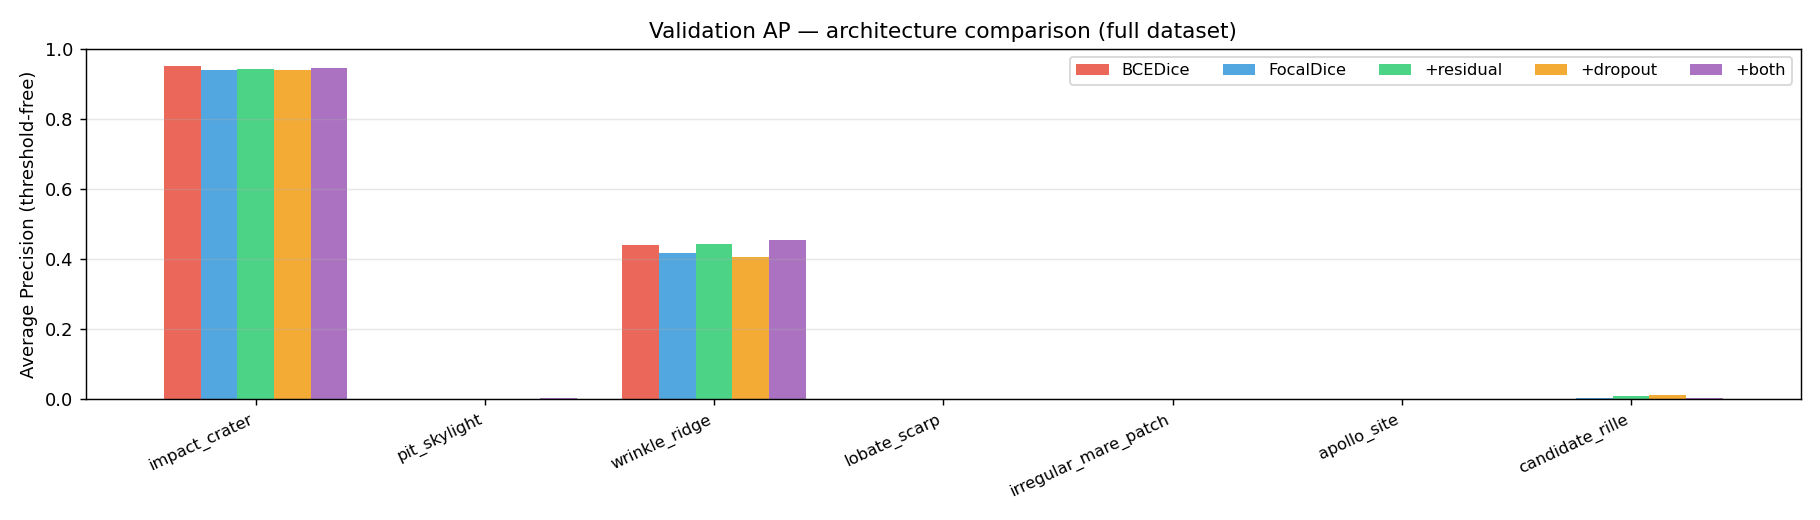
\includegraphics[width=\textwidth]{figures/MR/cloudveneto_arch_val_ap.png}
    \caption{Validation AP}
\end{subfigure}
\caption{Per-class validation metrics across training epochs for the five architecture configurations (full T4 run, 30 epochs). \textbf{+both} (residual + dropout + FocalDice) achieves the highest aggregate performance on all three metrics.}
\label{fig:arch_metrics}
\end{figure}

\paragraph{Key findings.}
Residual shortcuts consistently improve over the plain DoubleConv baseline on aggregate F1, IoU, and AP (+residual vs FocalDice: $+0.0071$ mean F1, $+0.0050$ mean AP). Dropout alone does not help — it degrades both mean AP and ridge AP relative to plain FocalDice, likely because sparse labels already act as a strong regulariser. The combination \textbf{+both} achieves the best mean F1 (0.2076), best mean IoU (0.1688), and best mean AP (0.2004), as well as the highest ridge AP (0.453). Impact-crater AP is uniformly high (0.939–0.951) across all configurations, but given the 0.821 prevalence baseline (Table~\ref{tab:prevalence}) this represents only a modest lift over chance; the architecture choice matters primarily for rare and structurally subtle classes such as ridges, where AP~0.44--0.45 is ${\sim}70\times$ the 0.0064 chance level.

% -----------------------------------------------------------------------------
\subsection{Study 2 — Network Width}
\label{sec:mr_width}

Using the best architecture from Study~1 (\textbf{+both}: FocalDice + residual + dropout=0.3), we sweep the base width $w \in \{16, 32, 64\}$, corresponding to 505K, 2.0M, and 8.0M parameters respectively.

\begin{table}[h]
\centering
\caption{Base-width sweep (FocalDice + residual + dropout=0.3, full T4 run, 30 epochs).}
\label{tab:bw_comparison}
\begin{tabular}{lrrrrrr}
\toprule
Config & Params & Epoch (s) & Mean F1 & Mean IoU & Mean AP & Ridge AP \\
\midrule
small ($w=16$)   &    505{,}095 &  139 & 0.2031 & 0.1665 & 0.2003 & 0.451 \\
default ($w=32$) & 2{,}014{,}727 &  258 & 0.2093 & 0.1704 & 0.2010 & 0.456 \\
wide ($w=64$)    & 8{,}047{,}623 &  582 & \textbf{0.2153} & \textbf{0.1733} & \textbf{0.2016} & 0.445 \\
\bottomrule
\end{tabular}
\end{table}

\begin{figure}[h]
\centering
\begin{subfigure}[b]{0.32\textwidth}
    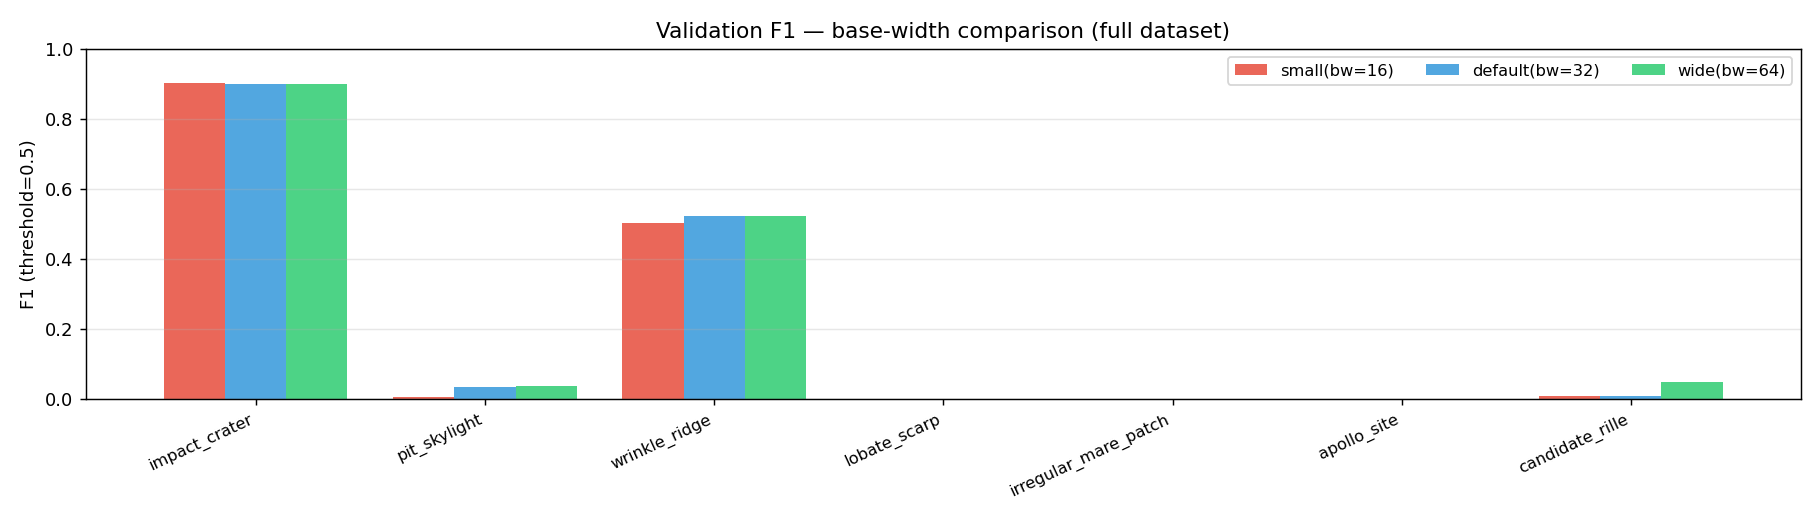
\includegraphics[width=\textwidth]{figures/MR/cloudveneto_bw_val_f1.png}
    \caption{Validation F1}
\end{subfigure}
\hfill
\begin{subfigure}[b]{0.32\textwidth}
    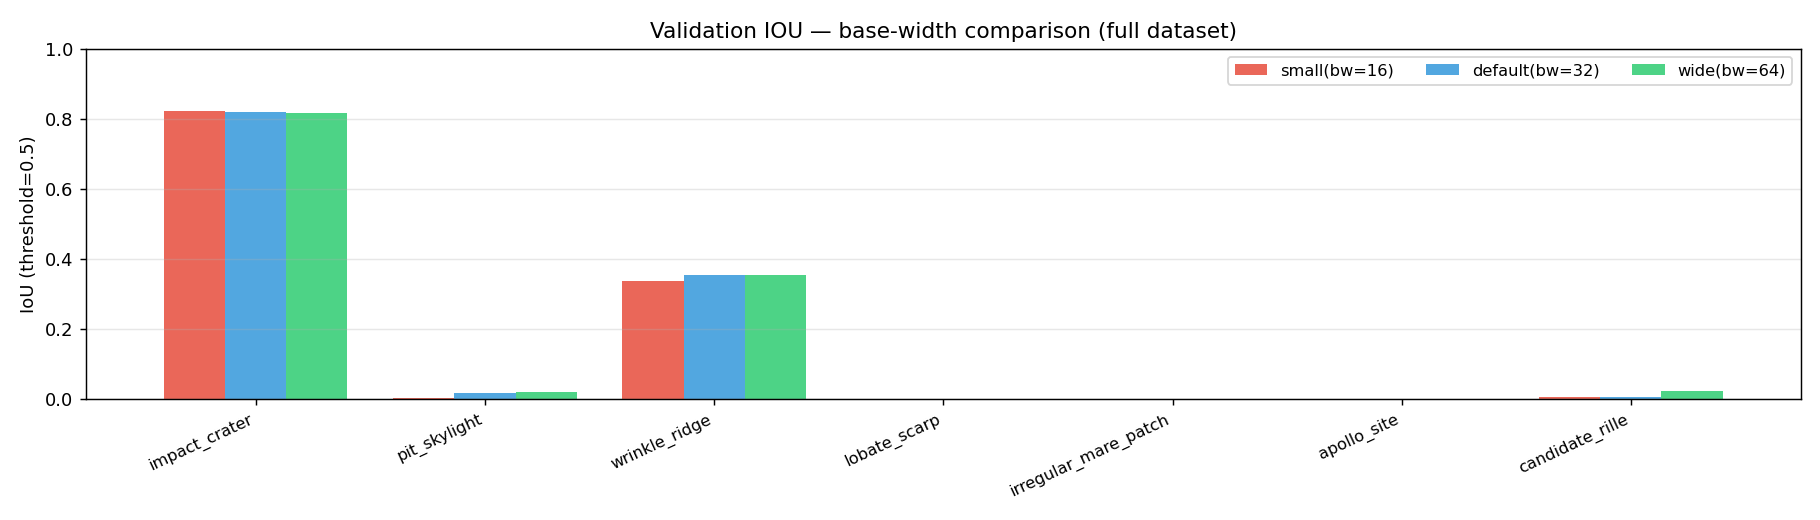
\includegraphics[width=\textwidth]{figures/MR/cloudveneto_bw_val_iou.png}
    \caption{Validation IoU}
\end{subfigure}
\hfill
\begin{subfigure}[b]{0.32\textwidth}
    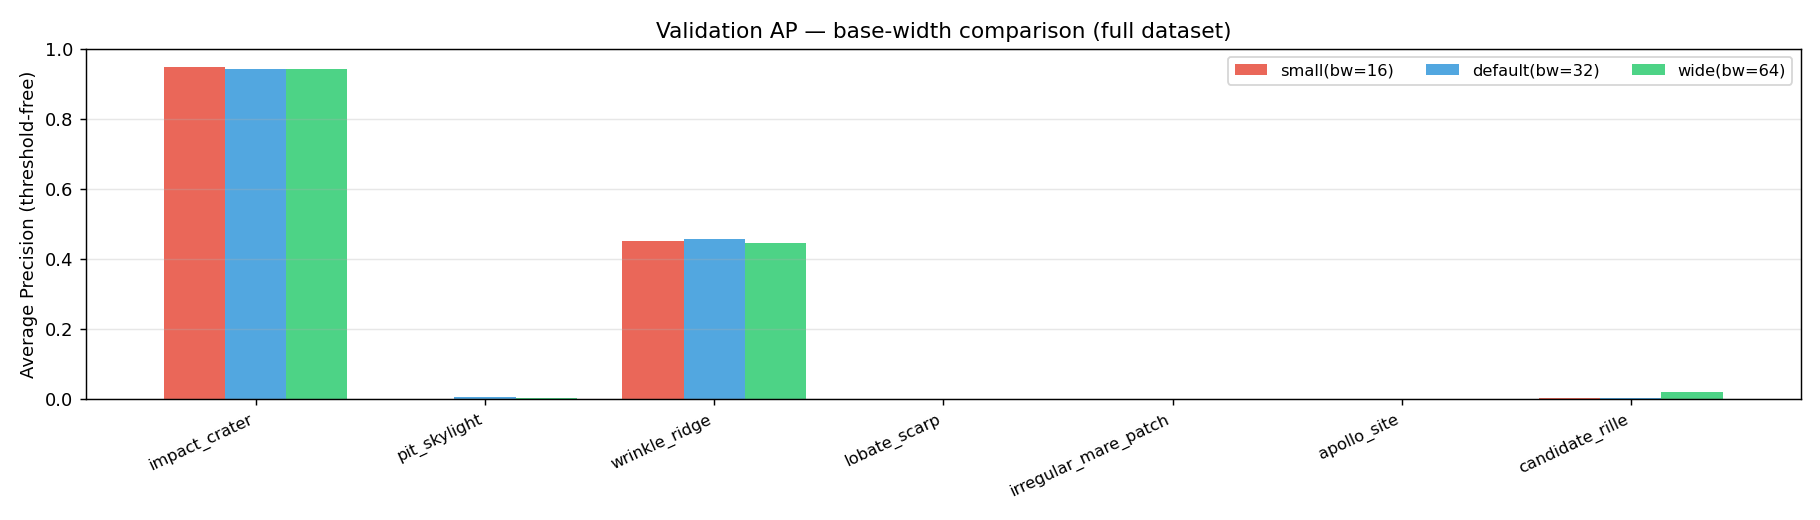
\includegraphics[width=\textwidth]{figures/MR/cloudveneto_bw_val_ap.png}
    \caption{Validation AP}
\end{subfigure}
\caption{Validation metrics for three network widths (full T4 run, 30 epochs). Wider networks achieve marginally higher scores but exhibit severely diminishing returns in terms of parameters and training time.}
\label{fig:bw_metrics}
\end{figure}

\paragraph{Key findings.}
The wide model ($w=64$) achieves the best mean AP (0.2016) and mean F1 (0.2153), but the improvement over the default ($w=32$) is marginal: $+0.0006$ mean AP, $+0.006$ mean F1, at the cost of a 4$\times$ parameter increase and a ${\sim}2.3\times$ increase in training time per epoch (258 s $\to$ 582 s). Strikingly, the small model ($w=16$) with only 505K parameters achieves a mean AP of 0.2003 — within 0.001 of the 8M-parameter wide model — making it the most parameter-efficient option. For deployment on resource-constrained hardware the small model offers the best trade-off.

% -----------------------------------------------------------------------------
\subsection{Study 3 — Data Augmentation}
\label{sec:mr_augmentation}

Using \textbf{+both} at $w=32$, we isolate the effect of geometric augmentation. The augmented pipeline applies random horizontal and vertical flips and 90°/180°/270° rotations to training tiles. No augmentation is applied to validation.

\begin{table}[h]
\centering
\caption{Augmentation study (FocalDice + residual + dropout=0.3, $w=32$, full T4 run, 30 epochs). Crater AP is given for reference; Ridge AP highlights the most affected rare class.}
\label{tab:aug_comparison}
\begin{tabular}{lrrrrrr}
\toprule
Config & Final loss & Mean F1 & Mean IoU & Mean AP & Crater AP & Ridge AP \\
\midrule
\textbf{no augmentation} & \textbf{3.698} & \textbf{0.2986} & \textbf{0.2289} & \textbf{0.2647} & \textbf{0.947} & \textbf{0.558} \\
+augmentation            &        3.863  &        0.2124  &        0.1724  &        0.2027  &        0.942  &        0.457  \\
\bottomrule
\end{tabular}
\end{table}

\begin{figure}[h]
\centering
\begin{subfigure}[b]{0.32\textwidth}
    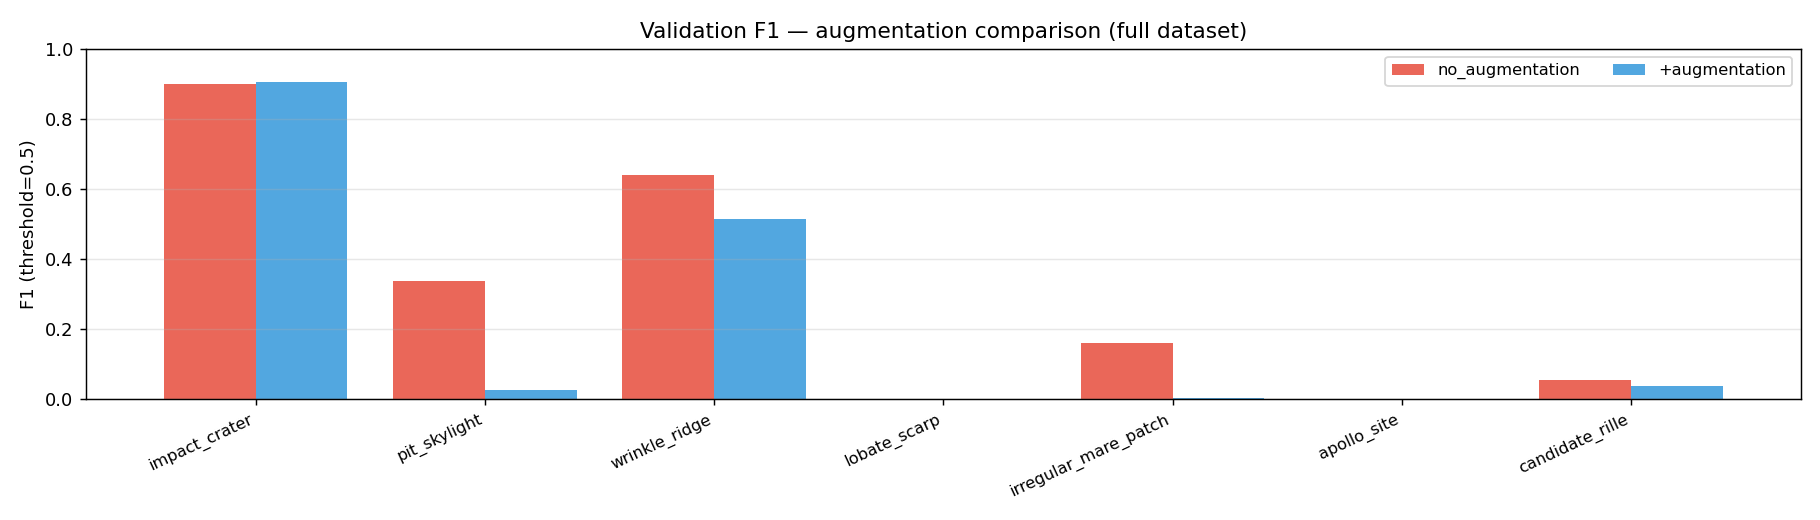
\includegraphics[width=\textwidth]{figures/MR/cloudveneto_aug_val_f1.png}
    \caption{Validation F1}
\end{subfigure}
\hfill
\begin{subfigure}[b]{0.32\textwidth}
    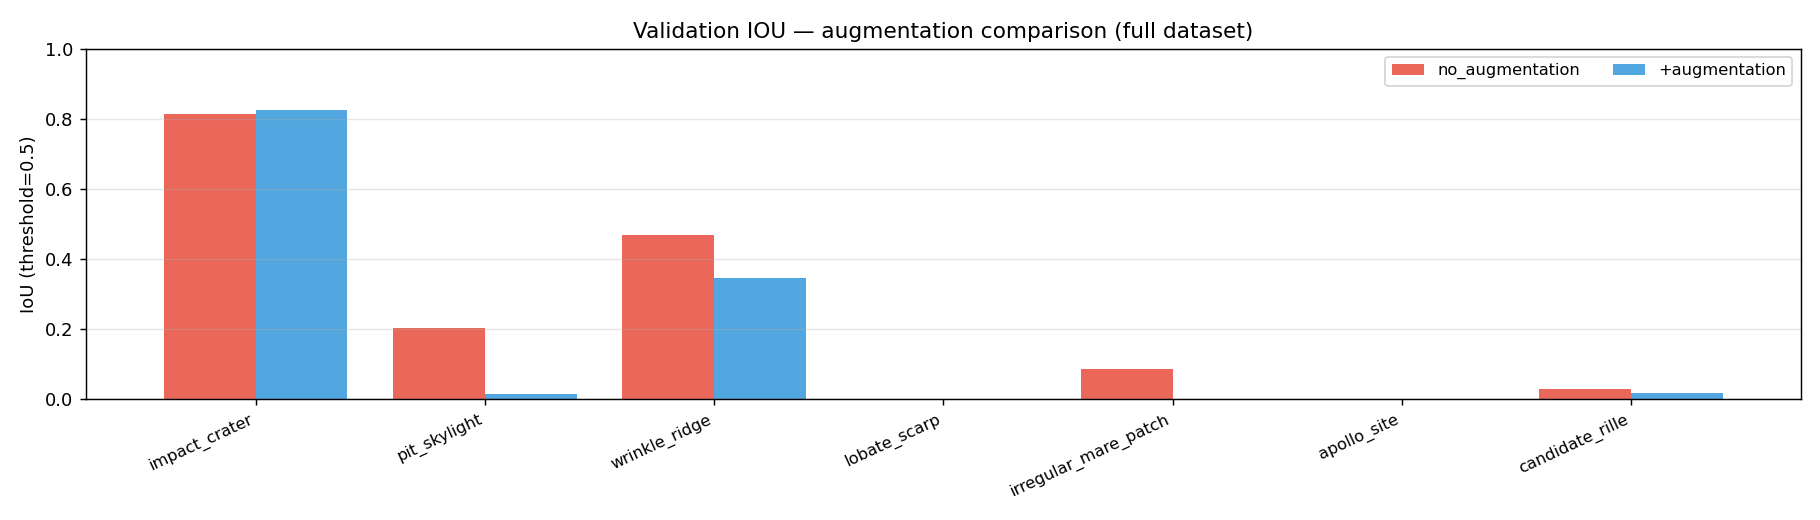
\includegraphics[width=\textwidth]{figures/MR/cloudveneto_aug_val_iou.png}
    \caption{Validation IoU}
\end{subfigure}
\hfill
\begin{subfigure}[b]{0.32\textwidth}
    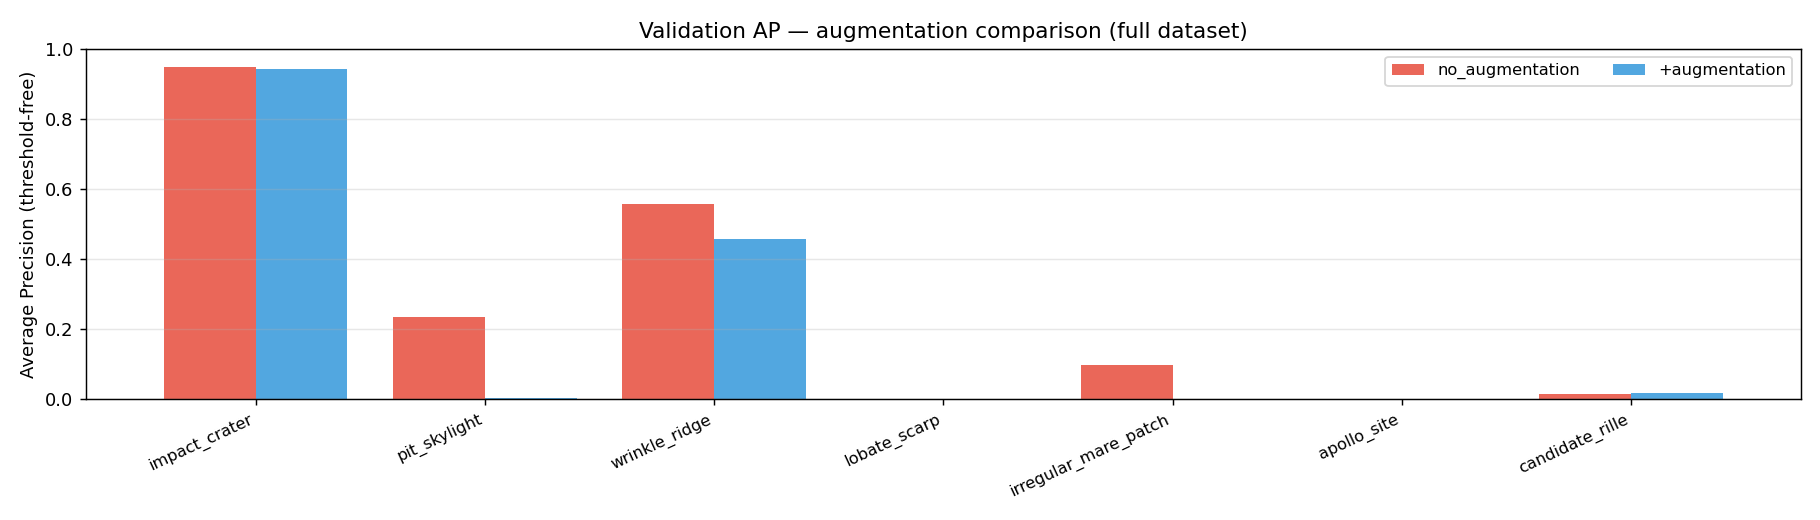
\includegraphics[width=\textwidth]{figures/MR/cloudveneto_aug_val_ap.png}
    \caption{Validation AP}
\end{subfigure}
\caption{Validation metrics with and without geometric augmentation (full T4 run, 30 epochs). No augmentation outperforms the augmented training on all metrics.}
\label{fig:aug_metrics}
\end{figure}

\paragraph{Key findings.}
This is the most striking result of the ablation campaign. Training without augmentation produces a model that is dramatically better on every metric: mean F1 improves by 0.086 (40\% relative), mean AP improves by 0.062 (31\% relative), and ridge AP improves from 0.457 to 0.558 (22\% relative).

Two effects plausibly combine to produce this result, and the present experiment cannot fully separate them.

First, a \emph{geological} effect: the Marius Hills region has a strong directional bias — wrinkle ridges run predominantly in a narrow range of orientations dictated by the regional stress field, and rilles follow the same orientation. Moreover, the Sun azimuth is consistent within the WAC mosaic, so flips and $90°$ rotations also produce illumination directions that never occur in the data. Applying such transforms presents the model with feature orientations and shading that are physically absent in the training region, injecting false diversity. Generic augmentation implicitly assumes that the transformed inputs remain representative of the target distribution~\cite{shorten2019augmentation}, an assumption violated here — the course material itself cautions against ``arbitrary rotations if illumination direction carries physical meaning''~\cite{zingales2026lecture}. Impact craters, being rotationally symmetric, are unaffected, which explains why crater AP is nearly identical in both conditions (0.947 vs 0.942).

Second, a \emph{methodological} confound: as noted in Sec.~\ref{sec:mr_dataset}, the random tile split leaks overlapping pixels into validation. A model trained without augmentation is freer to memorise tile appearance and is rewarded for it on a leaky split, while augmentation suppresses exactly this memorisation. Part of the measured gap could therefore be an artefact of the split rather than a property of the data. To separate the two effects, the comparison was re-run under the leakage-free spatial block split.

\paragraph{Leakage-free re-run.}
The augmentation pair was re-trained with \texttt{spatial\_train\_val\_split}: both arms share an identical pixel-disjoint split, the same initialisation seed, and the same cosine schedule, so the \emph{only} difference between them is augmentation. The re-run used a scaled paired protocol on local hardware (10{,}000 tiles, 30 epochs; a paired comparison remains internally valid at reduced scale), with a smaller 6{,}000-tile/15-epoch run giving consistent results. Table~\ref{tab:spatial_rerun} and Figure~\ref{fig:spatial_rerun} report the outcome.

\begin{table}[h]
\centering
\caption{Augmentation ablation under the leakage-free spatial split (10{,}000 tiles, 30 epochs, paired arms). \texttt{candidate\_rille} has zero positive pixels in the spatial validation set and is excluded from the macro averages (reported as NaN with zero support).}
\label{tab:spatial_rerun}
\begin{tabular}{lrrrr}
\toprule
Config & Mean F1 & Mean AP & Ridge F1 & Ridge AP \\
\midrule
\textbf{no augmentation} & \textbf{0.2294} & \textbf{0.2239} & \textbf{0.4586} & \textbf{0.3847} \\
+augmentation            &        0.2208  &        0.2096  &        0.3970  &        0.3060  \\
\bottomrule
\end{tabular}
\end{table}

\begin{figure}[h]
\centering
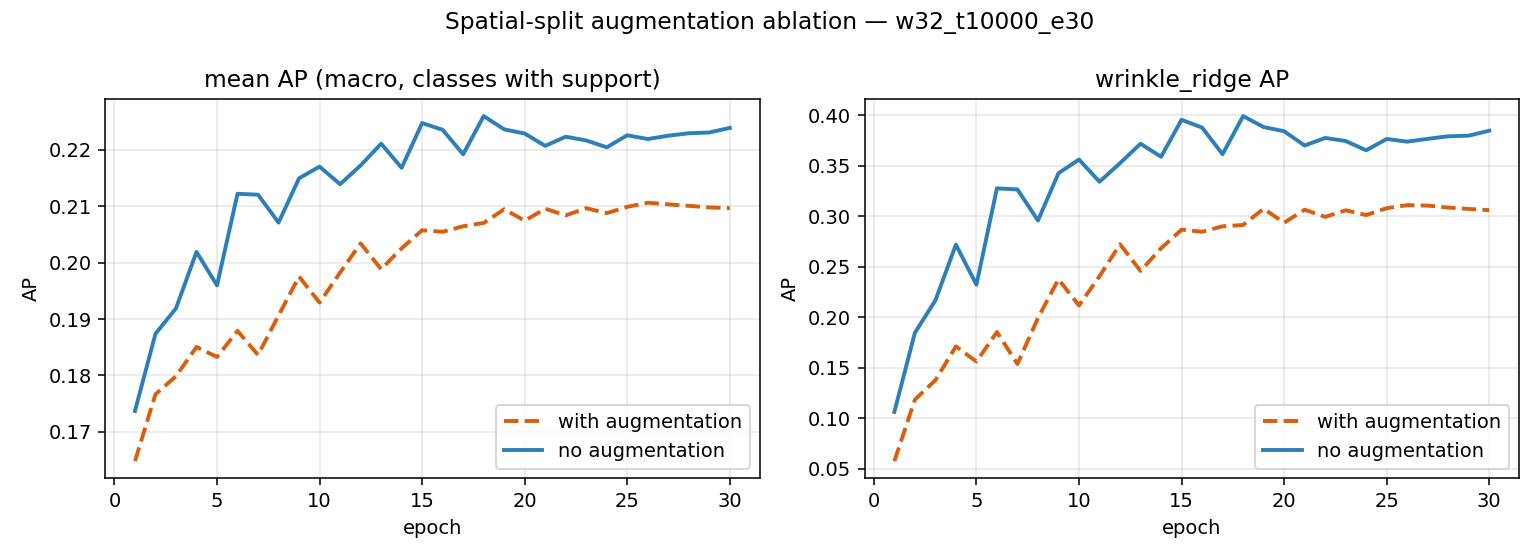
\includegraphics[width=\textwidth]{figures/MR/spatial_w32_t10000_e30_val_ap.png}
\caption{Validation AP across training epochs under the spatial split (macro mean over classes with support, left; \texttt{wrinkle\_ridge}, right). The no-augmentation arm dominates at every epoch on both metrics.}
\label{fig:spatial_rerun}
\end{figure}

The re-run \textbf{confirms the conclusion}: training without augmentation remains better, with the no-augmentation arm above the augmented one at every epoch (Fig.~\ref{fig:spatial_rerun}). The decomposition is, however, instructive. Absolute scores are substantially lower than on the leaky split (ridge AP 0.385 vs 0.558), confirming that random-split numbers were inflated by memorisation. The \emph{aggregate} advantage of no-augmentation also narrows (mean AP $+0.014$ here vs $+0.062$ on the leaky split), showing that part of the originally measured gap was indeed a split artefact. But for the direction-sensitive class the gap persists and is large — ridge AP 0.385 vs 0.306, a 26\% relative difference on strictly disjoint validation pixels — which is precisely the signature predicted by the geological explanation: augmentation hurts where orientation and illumination carry physical information. Confirmation at the full 15{,}931-tile T4 protocol remains scheduled, but the conclusion no longer rests on a confounded measurement.

% -----------------------------------------------------------------------------
\subsection{Qualitative Evaluation}
\label{sec:mr_qualitative}

Segmentation metrics alone do not reveal \emph{how} a model fails, so we complement the ablations with a visual comparison on identical validation tiles: raw image, ground truth, predicted probability, and a true-positive/false-positive/false-negative decomposition at threshold $0.5$, for the BCEDice baseline and the definitive model side by side (generated by \texttt{scripts/qualitative\_eval.py}; tiles are the three validation tiles with the largest \texttt{wrinkle\_ridge} ground-truth area).

\begin{figure}[h]
\centering
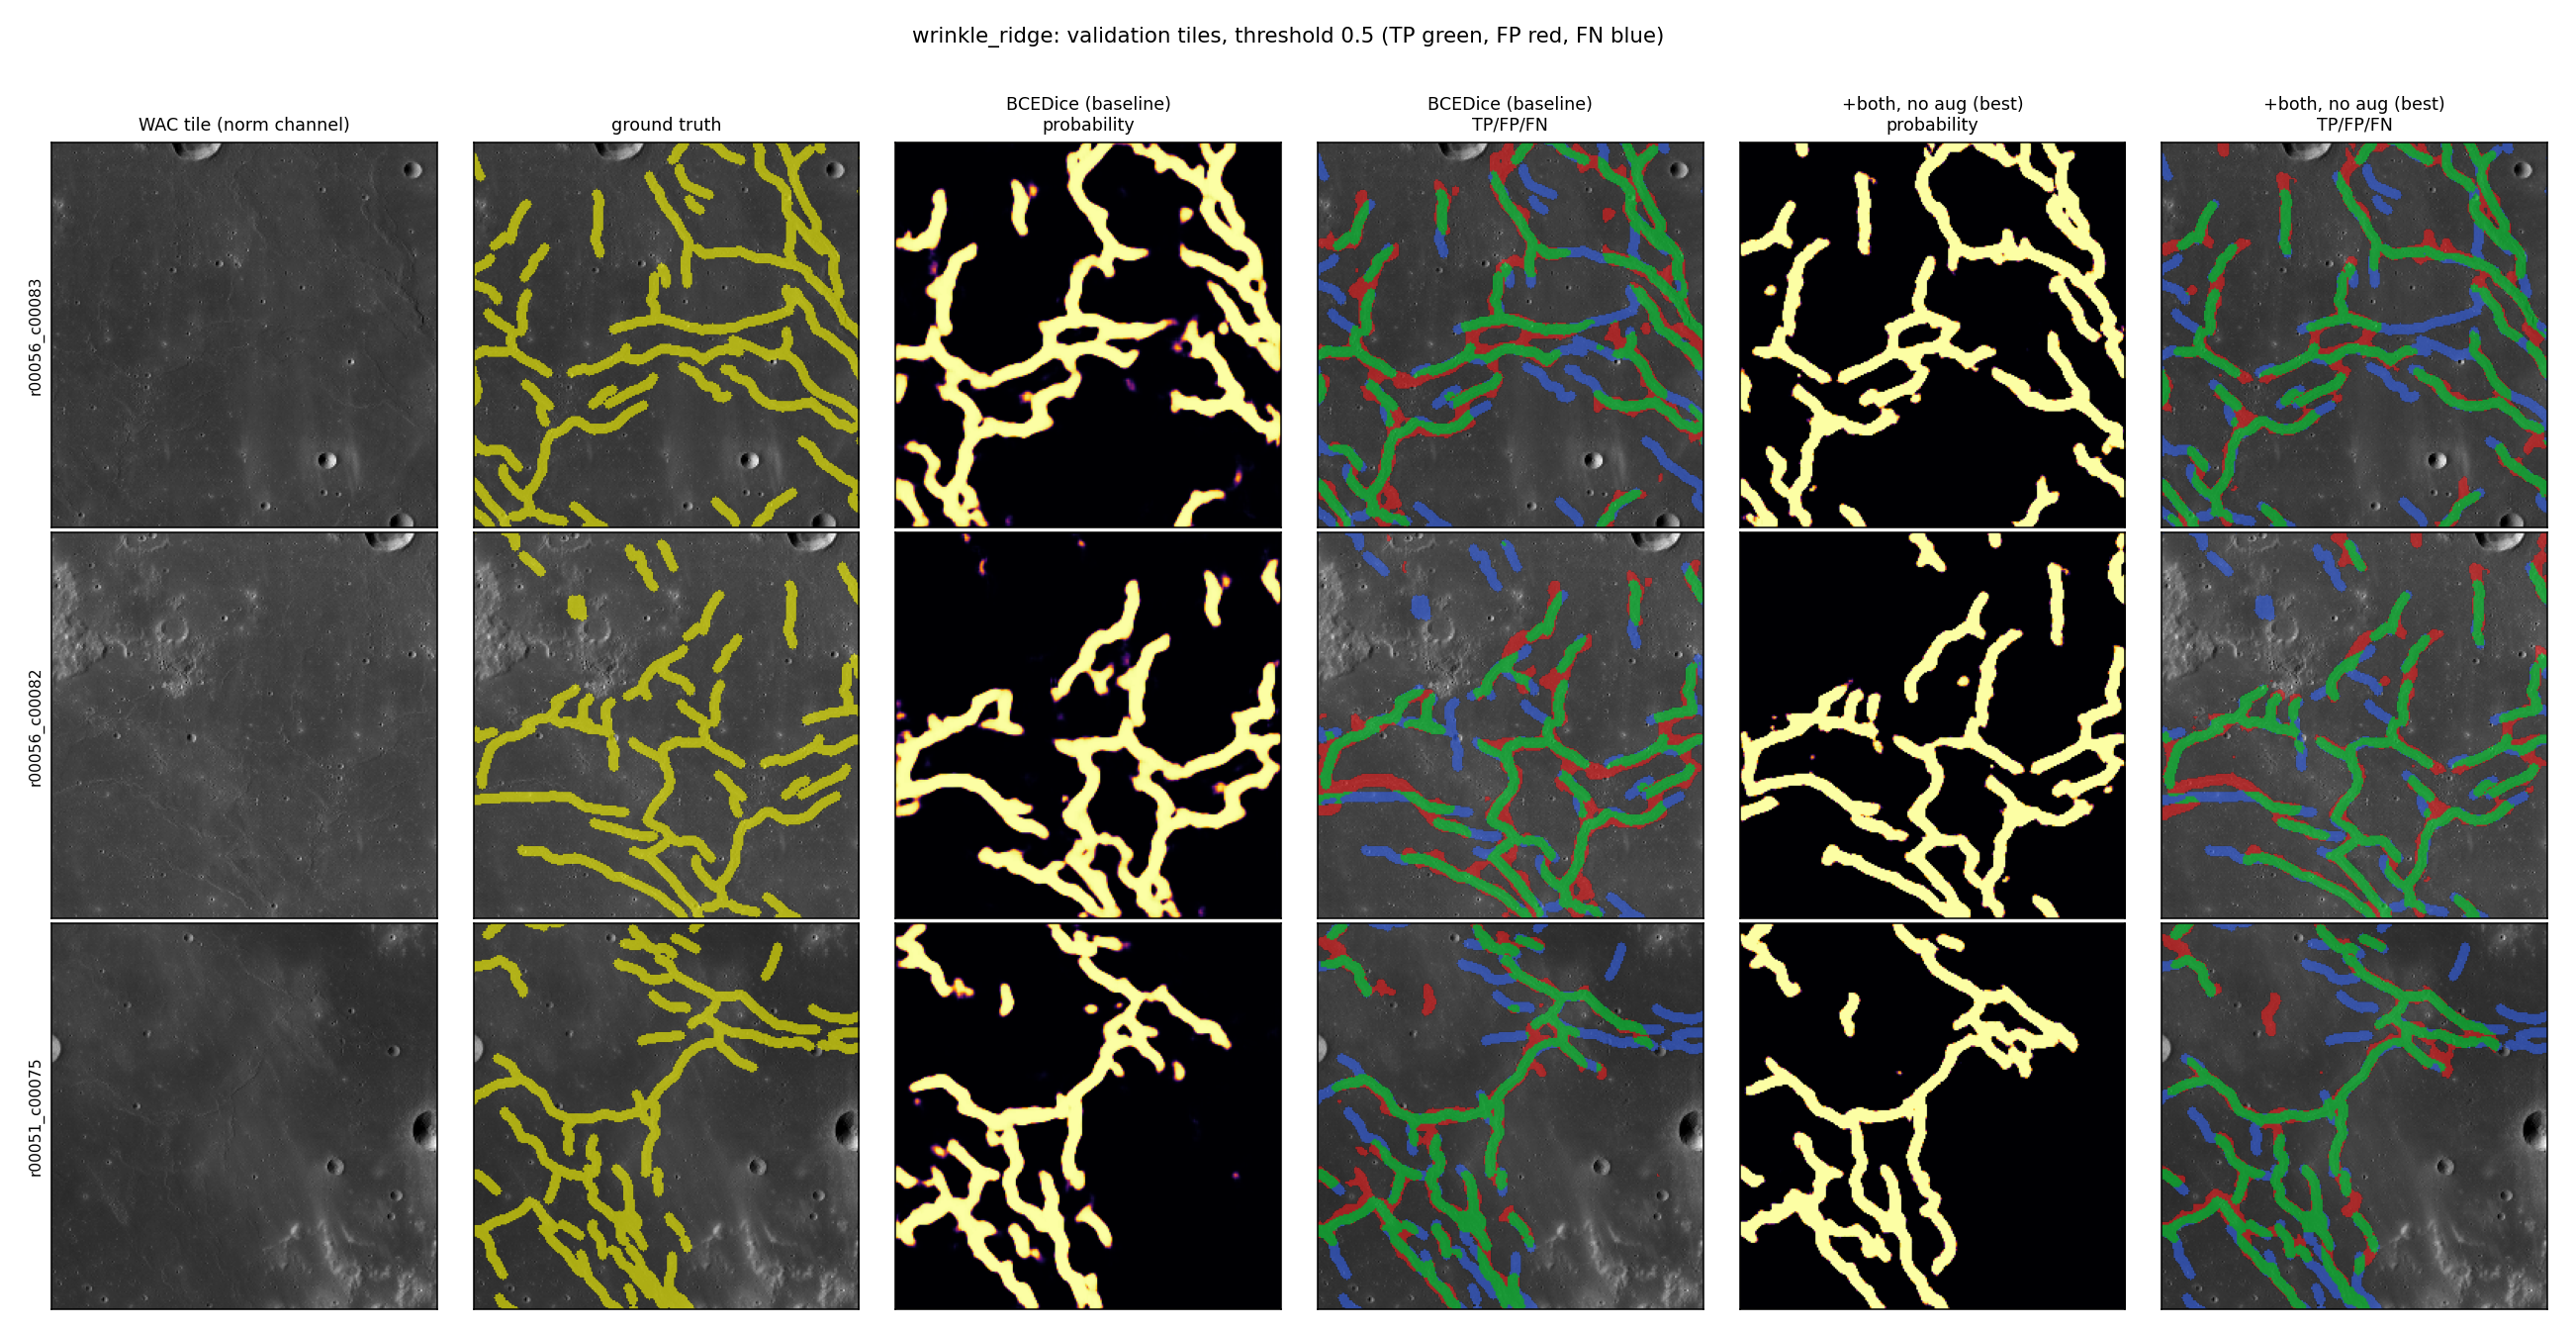
\includegraphics[width=\textwidth]{figures/MR/qualitative_wrinkle_ridge.png}
\caption{Wrinkle-ridge qualitative comparison on three validation tiles (TP green, FP red, FN blue). Both models recover the topology of the ridge network; the definitive model (+both, no augmentation) produces visibly more complete coverage and fewer false positives than the BCEDice baseline. Errors concentrate on thin, low-contrast ridge segments, consistent with the localisation difficulty of linear features.}
\label{fig:qualitative_ridge}
\end{figure}

\begin{figure}[h]
\centering
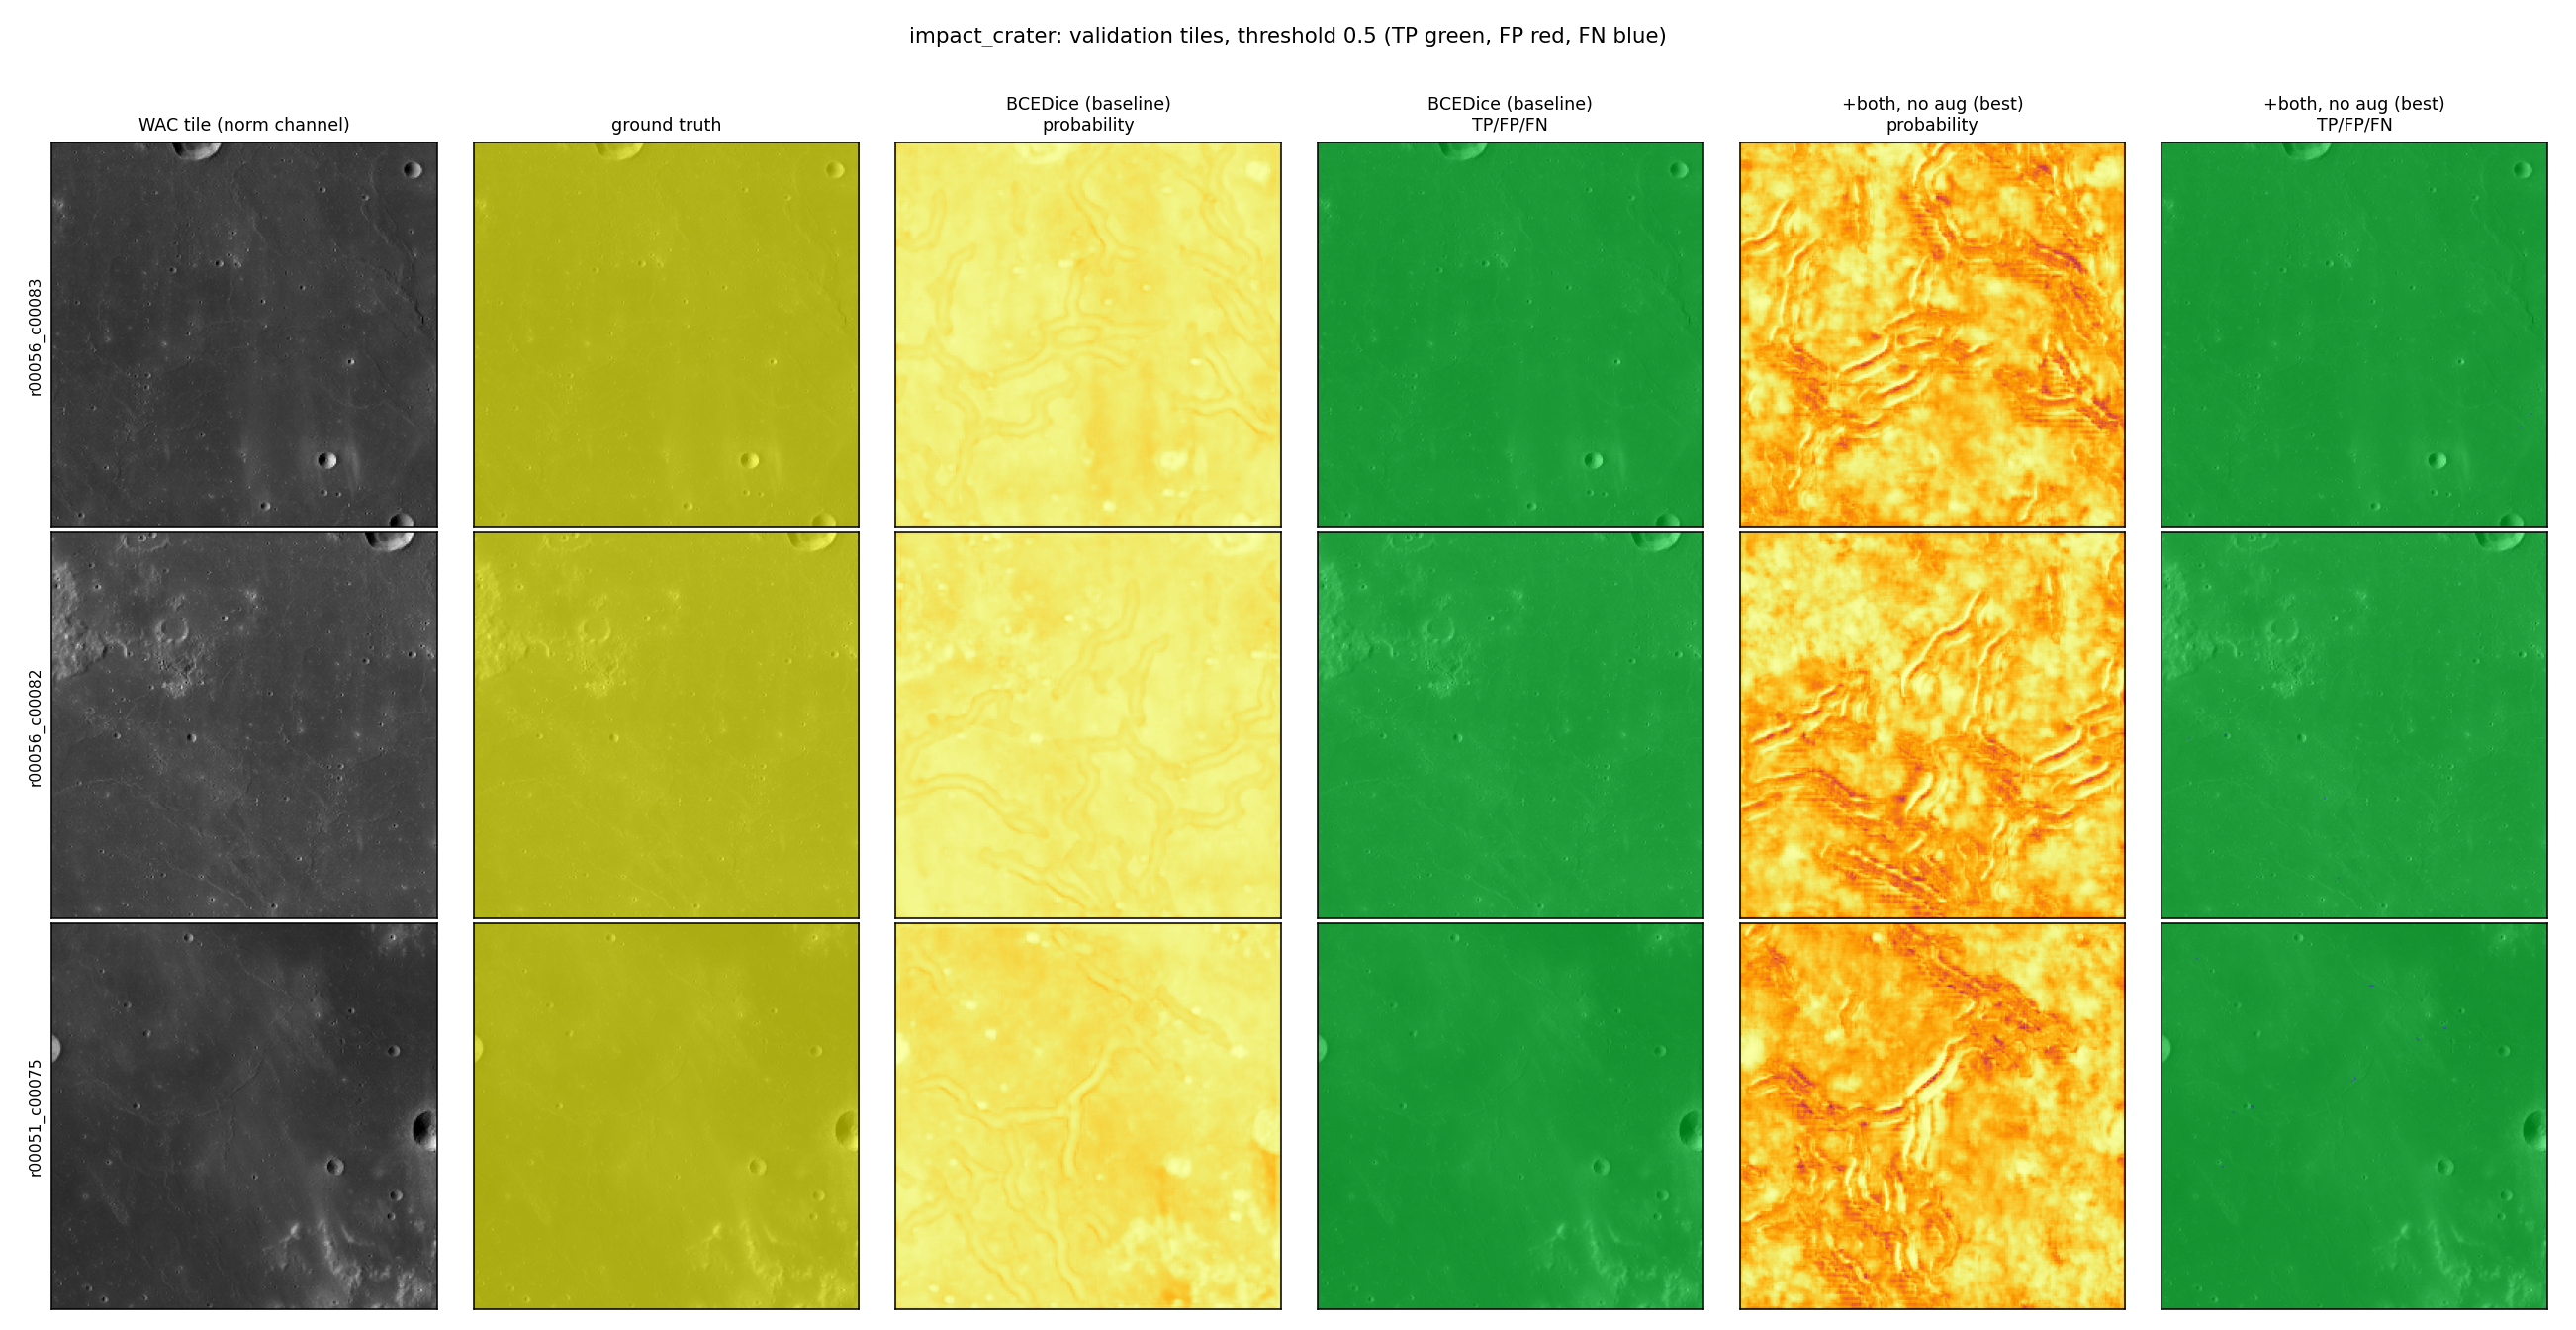
\includegraphics[width=\textwidth]{figures/MR/qualitative_impact_crater.png}
\caption{Impact-crater qualitative comparison on the same tiles. The ground truth covers the \emph{entire} tile (cf.\ the 82\% prevalence and 50.7\% fully-covered tiles of Table~\ref{tab:prevalence}), so a prediction of ``everywhere'' is trivially correct: this figure is direct visual evidence that the crater channel behaves as a near-coverage layer and that crater AP must be read against its 0.821 chance baseline.}
\label{fig:qualitative_crater}
\end{figure}

The ridge comparison shows that the metric gains of the definitive model correspond to a real, visible improvement in completeness of the recovered ridge network. The crater comparison, conversely, makes the saturation argument of Sec.~\ref{sec:mr_dataset} concrete.

% -----------------------------------------------------------------------------
\subsection{South Pole Inference}
\label{sec:mr_south_pole}

The best-performing model weights (\texttt{best\_trained.pth}) were applied to the lunar south pole to demonstrate transfer beyond the training region. The south pole imagery was obtained from the same LRO WAC source and tiled identically, producing 3{,}639 tiles.

\paragraph{Inference pipeline.}
Each tile is preprocessed with the same CLAHE + Sobel three-channel pipeline. A sliding-window predictor runs the model tile by tile, saving per-class probability maps as compressed \texttt{.npz} files for downstream aggregation. Probability maps are aggregated over all tiles to compute global statistics.

\paragraph{Per-class results.}
Table~\ref{tab:south_pole_stats} reports the aggregated statistics over the 3{,}639 south pole tiles.

\begin{table}[h]
\centering
\caption{South pole inference results (3{,}639 tiles). Avg.\ Max.\ Prob.\ is the mean, over tiles, of the maximum predicted probability for each class. Global Max is the highest probability observed in any single tile. A high avg.\ max but low global max indicates diffuse, uncertain detections; a high global max but low avg.\ max indicates rare but confident detections.}
\label{tab:south_pole_stats}
\begin{tabular}{lrrr}
\toprule
Class & Avg.\ Max.\ Prob. & Global Max & Status \\
\midrule
\texttt{impact\_crater}       & 0.863 & 1.000 & \checkmark\ detected \\
\texttt{lobate\_scarp}        & 0.060 & 0.303 & weak \\
\texttt{pit\_skylight}        & 0.051 & 0.202 & weak \\
\texttt{irregular\_mare\_patch} & 0.040 & 0.215 & weak \\
\texttt{apollo\_site}         & 0.040 & 0.183 & weak \\
\texttt{candidate\_rille}     & 0.006 & 0.480 & sparse \\
\texttt{wrinkle\_ridge}       & 0.001 & 1.000 & sparse \\
\bottomrule
\end{tabular}
\end{table}

\begin{figure}[h]
\centering
\begin{subfigure}[b]{0.48\textwidth}
    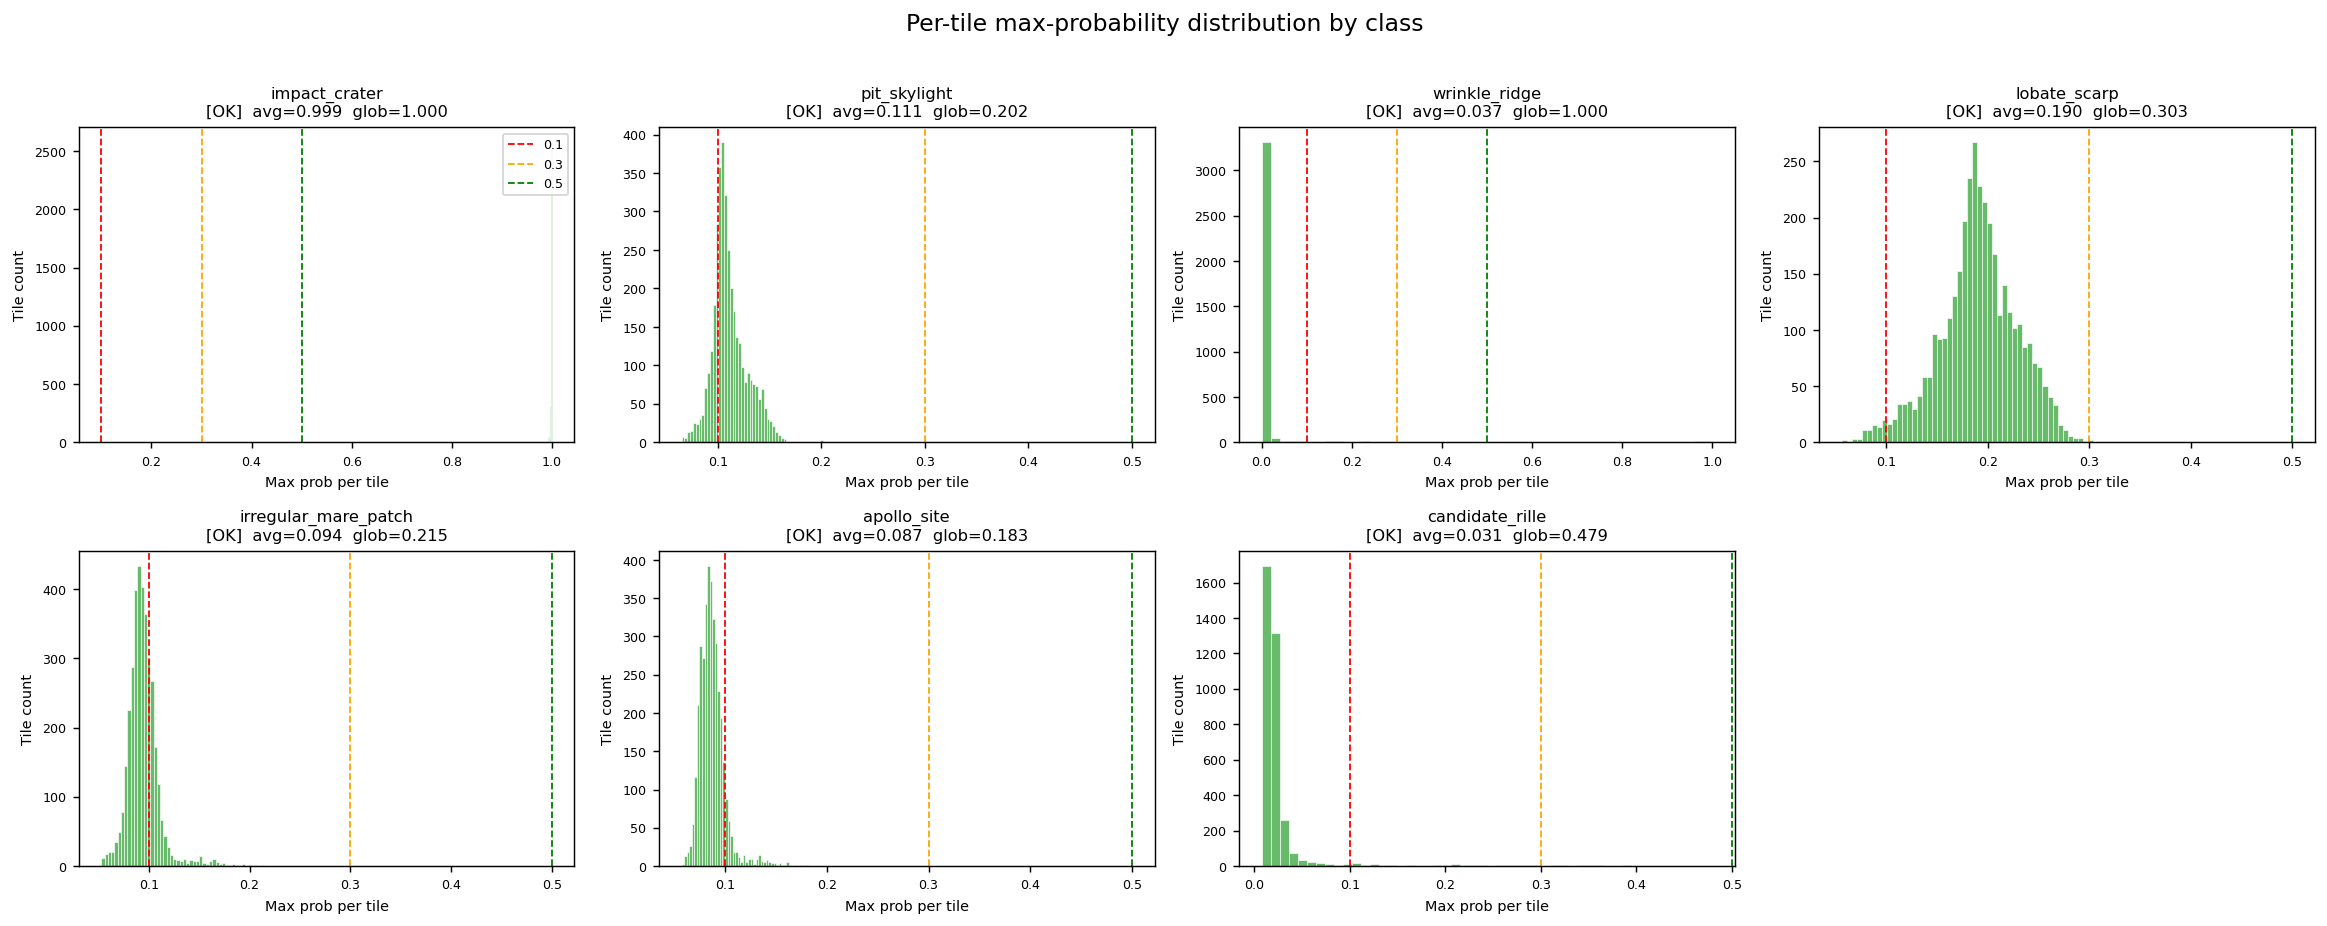
\includegraphics[width=\textwidth]{figures/MR/diagnostics_distributions.png}
    \caption{Per-tile max-probability distributions.}
\end{subfigure}
\hfill
\begin{subfigure}[b]{0.48\textwidth}
    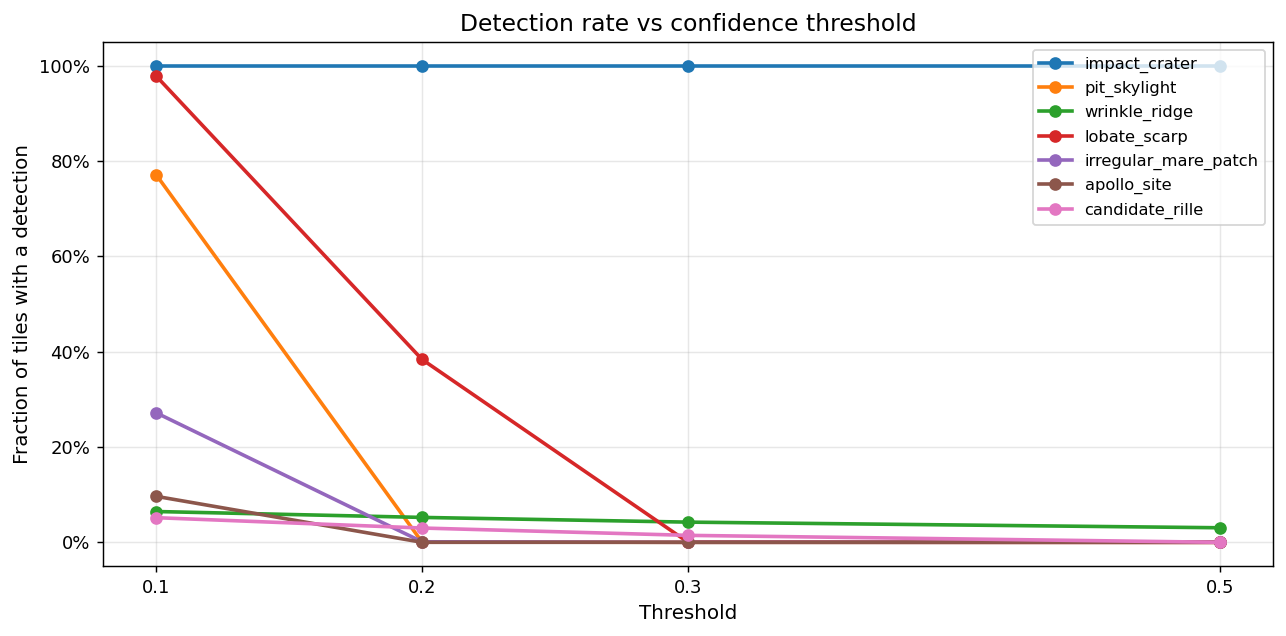
\includegraphics[width=\textwidth]{figures/MR/diagnostics_detection_rates.png}
    \caption{Detection rate vs.\ confidence threshold.}
\end{subfigure}
\caption{South pole inference diagnostics across 3{,}639 tiles. Impact craters are detected with near-certainty across the entire region. All other classes exhibit strongly right-skewed distributions with low average confidence, reflecting both the domain shift from Marius Hills and the scarcity of these features at the south pole.}
\label{fig:south_pole_diag}
\end{figure}

\begin{figure}[h]
\centering
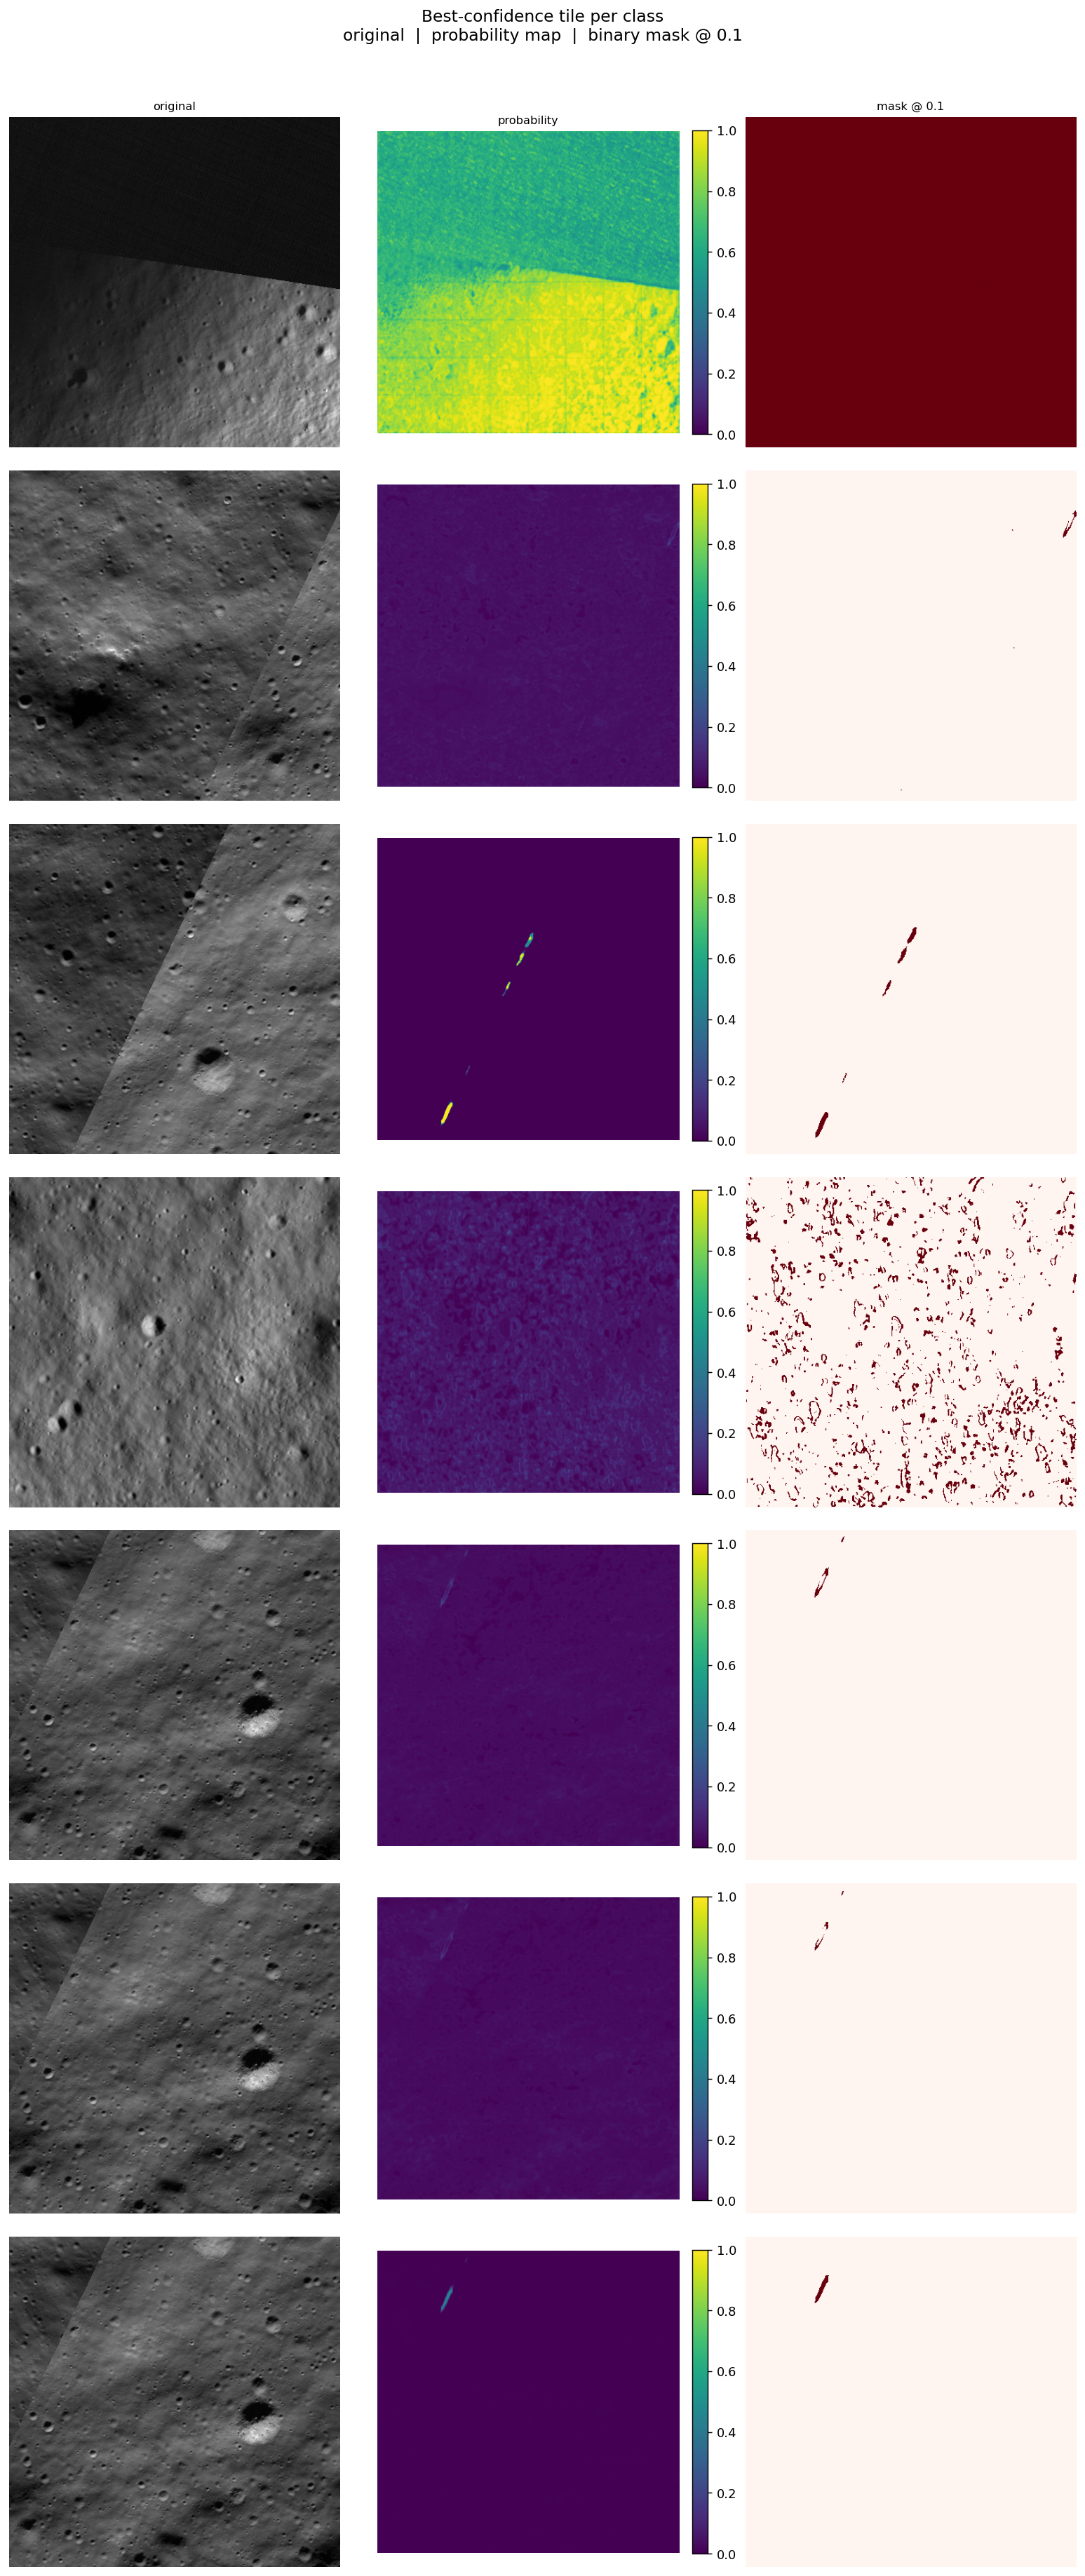
\includegraphics[width=\textwidth, height=0.82\textheight, keepaspectratio]{figures/MR/diagnostics_best_tiles.png}
\caption{Best-detected tile per class on the south pole imagery. Each panel shows the LRO WAC tile overlaid with the predicted probability map for the class with the highest maximum confidence in that tile. Note that overlays use a \emph{relative} threshold (top fraction of each tile's probabilities) so that the most likely candidate pixels are visible even when absolute confidence is low; coloured regions for the weak classes are therefore candidate locations, not confident detections. Impact craters stand out clearly; other classes show localised but low-confidence activations.}
\label{fig:south_pole_best}
\end{figure}

\paragraph{Analysis.}
The model assigns high crater probability across the entire south pole (average max probability 0.863). Given the near-saturated crater layer learned in training (Sec.~\ref{sec:mr_dataset}), this is expected behaviour — the model has learned that almost everywhere is ``crater'' — and should not be over-interpreted as precise crater delineation. Two classes — \texttt{wrinkle\_ridge} and \texttt{candidate\_rille} — show an interesting pattern: very low average-tile probabilities (0.001 and 0.006) but anomalously high global maxima (1.000 and 0.480). This indicates that the model makes rare but high-confidence predictions on a small number of tiles, rather than diffuse low-confidence activations everywhere.

The weak performance on rare classes at the south pole is attributable to two combined factors. First, the south pole is geologically distinct from Marius Hills: it lacks the volcanic structures (skylights, rilles, ridges) that dominate the training distribution, making it an out-of-distribution region for those classes. Second, the extremely low frequency of those classes in the training data means the model has seen very few positive examples even during Marius Hills training. Both issues motivate future work on label-efficient transfer learning and domain adaptation.

% -----------------------------------------------------------------------------
\subsection{Methodological Audit and Reproducibility}
\label{sec:mr_audit}

After the experimental campaign was completed, the entire pipeline — code, data, report claims, and course guidance — was subjected to a systematic audit. Every resulting change is a single, individually justified commit on the \texttt{U-net} branch, indexed in \texttt{Moon-Recognition/IMPROVEMENTS.md}; the executed notebooks were committed \emph{before} any fix, so the provenance of the published numbers is preserved. This section summarises what the audit found and how each finding affects the interpretation of the results — both as a record for the group and because several findings changed the conclusions of this report.

\paragraph{(a) Report--code reconciliation.}
Several statements in an earlier draft did not match the implementation and were corrected against the code as ground truth: the CLAHE parameters (the pipeline uses \texttt{skimage} \texttt{equalize\_adapthist} with clip limit 0.03, not the OpenCV-style values previously quoted), the tiling description (tiles \emph{overlap} by 50\%), the split procedure (random permutation, not sequential), a gradient-clipping claim (clipping was never enabled), and a mis-attributed citation in the augmentation discussion (replaced with the correct survey~\cite{shorten2019augmentation}). The principle applied: any claim an examiner can check against the repository must be checkable.

\paragraph{(b) Train/validation leakage --- discovery and remedy.}
Because adjacent tiles share 50\% of their pixels, the random tile-level split leaks: a direct measurement on the real index showed that \textbf{100\% of the 3{,}186 validation tiles overlap at least one training tile}. This inflates absolute validation scores and specifically confounds the augmentation study, since a non-augmented model is freer to memorise tile appearance and a leaky validation set rewards exactly that memorisation. The remedy, recommended by the course material itself, is a \emph{spatial block split}: contiguous $1024$-px blocks are assigned to validation and every training tile whose footprint intersects a validation tile is discarded ($\texttt{data/splits.py}$; on the real index: 11{,}289 train / 3{,}248 validation tiles, 1{,}394 boundary tiles dropped, zero pixel overlap, verified by an independent assertion). The augmentation comparison was re-run under this split as a scaled paired protocol on local hardware (both arms share an identical split, initialisation, and schedule, so the comparison is internally valid); the conclusion was confirmed, with the expected partial decomposition into a leakage artefact and a genuine effect (Sec.~\ref{sec:mr_augmentation}). Full-protocol confirmation on CloudVeneto remains scheduled when GPU instances become available.

\paragraph{(c) Label audit --- channel saturation.}
A full pass over all 15{,}931 tiles produced the per-class prevalences of Table~\ref{tab:prevalence} and the central reinterpretation of this report: the \texttt{impact\_crater} channel covers 82.1\% of all pixels, making it a near-coverage layer whose AP must be read against a 0.821 chance baseline, while \texttt{wrinkle\_ridge} (prevalence $6.4\times10^{-3}$) emerges as the strongest genuine result and the five rarest classes turn out to have essentially no supervision at all. Without this audit, the headline claim of the report would have been the (nearly trivial) crater result.

\paragraph{(d) Qualitative evaluation.}
The course material requires visual evaluation alongside metrics. Figures~\ref{fig:qualitative_ridge} and~\ref{fig:qualitative_crater} (generated by \texttt{scripts/qualitative\_eval.py} from the full-run checkpoints) confirm both audit findings visually: the metric advantage of the definitive model corresponds to a visibly more complete ridge reconstruction, and the crater ground truth fills entire tiles.

\paragraph{(e) Engineering fixes.}
The audit also produced functional fixes, each preserving the published numbers: evaluation memory reduced by ${\sim}12$\,GB with results verified bit-identical; undefined metrics for classes absent from a validation split now reported as NaN with an explicit support count rather than as a spurious 0; checkpoint loading made compatible with PyTorch $\geq 2.6$ and made loud on architecture/checkpoint mismatches (previously a mismatch silently produced random predictions); the sliding-window inference default aligned with the 256-px training context; dead machine-specific paths removed from the data manifest; and the training configuration file synchronised with the protocol actually used for the published runs.

% -----------------------------------------------------------------------------
\subsection{Summary and Conclusions}
\label{sec:mr_conclusions}

Table~\ref{tab:final_summary} collects the final T4 results for the best configuration identified in each study. The definitive model for the project is \textbf{SmallUNet with $w=32$, FocalDice loss, residual shortcuts, bottleneck dropout ($p=0.3$), trained without augmentation for 30 epochs on the full 15{,}931-tile Marius Hills dataset}. Its weights are stored as \texttt{data/MR/weights/best\_trained.pth}.

\begin{table}[h]
\centering
\caption{Best result from each ablation study (full T4 run, 30 epochs).}
\label{tab:final_summary}
\begin{tabular}{llrrrr}
\toprule
Study & Best config & Params & Mean F1 & Mean AP & Ridge AP \\
\midrule
Architecture & +both ($w=32$, augmented) & 2.0M & 0.2076 & 0.2004 & 0.453 \\
Width        & wide ($w=64$, augmented)  & 8.0M & 0.2153 & 0.2016 & 0.445 \\
Augmentation & +both, $w=32$, \textbf{no aug} & 2.0M & \textbf{0.2986} & \textbf{0.2647} & \textbf{0.558} \\
\bottomrule
\end{tabular}
\end{table}

The principal conclusions of this study are:

\begin{enumerate}
    \item \textbf{Residual shortcuts help; dropout alone does not.} Adding residual connections to DoubleConv blocks consistently improves all aggregate metrics. Bottleneck dropout in isolation hurts performance, likely because sparse labels already regularise the network. The combination \textbf{+both} yields the best augmented-training result.

    \item \textbf{Network width exhibits strong diminishing returns.} The small model ($w=16$, 505K parameters) achieves a mean AP within 0.001 of the wide model ($w=64$, 8M parameters) at one-sixth the training time and ${\sim}16\times$ fewer parameters. For resource-constrained inference the small model is recommended.

    \item \textbf{Geometric augmentation is harmful on this dataset — confirmed under a leakage-free split.} Training without flips and rotations outperforms the augmented model on the original random split, and the advantage survives the spatial block split re-run with strictly disjoint validation pixels (ridge AP 0.385 vs 0.306, no-augmentation above at every epoch). The decomposition is informative: part of the aggregate gap on the random split was a leakage artefact, but the direction-sensitive classes retain a large genuine gap, exactly as predicted by the directional bias of the Marius Hills linear features and the fixed illumination geometry. Augmentation strategies must be tailored to the structural properties of the target domain.

    \item \textbf{Crater AP must be read against its prevalence baseline; ridges are the strongest genuine result.} The \texttt{impact\_crater} channel covers 82.1\% of all pixels (half of the tiles are fully positive), so its AP $\approx 0.95$ is only a modest lift over the 0.821 chance level — the channel behaves as a near-coverage layer, and Fig.~\ref{fig:qualitative_crater} shows that predicting ``everywhere'' is trivially correct. By contrast, \texttt{wrinkle\_ridge} has a prevalence of $6.4\times10^{-3}$, so the best ridge AP of 0.558 is ${\sim}90\times$ chance level and corresponds to a visibly accurate reconstruction of the ridge network (Fig.~\ref{fig:qualitative_ridge}). The remaining five classes have prevalences below $1.4\times10^{-4}$ — their near-zero scores reflect the absence of supervision, not a failure of the architecture.

    \item \textbf{South pole transfer is limited by domain shift and label scarcity.} The model accurately maps impact craters but provides only weak signals for rarer geomorphological features. Acquiring labels for even a small number of south-pole-specific tiles, or employing few-shot domain adaptation, is likely necessary for reliable multi-class south-pole mapping.
\end{enumerate}

% Bibliography entries to add to the main .bib file:
% @inproceedings{ronneberger2015unet,
%   title={U-Net: Convolutional Networks for Biomedical Image Segmentation},
%   author={Ronneberger, Olaf and Fischer, Philipp and Brox, Thomas},
%   booktitle={MICCAI},
%   year={2015}
% }
% @inproceedings{lin2017focal,
%   title={Focal Loss for Dense Object Detection},
%   author={Lin, Tsung-Yi and Goyal, Priya and Girshick, Ross and He, Kaiming and Dollár, Piotr},
%   booktitle={ICCV},
%   year={2017}
% }
% @misc{zingales2026lecture,
%   author={Zingales, Tiziano},
%   title={Moon Features Recognition (Lecture 3b)},
%   howpublished={Computational Physics, Physics of Data, University of Padova},
%   year={2026}
% }
% @article{shorten2019augmentation,
%   title={A survey on Image Data Augmentation for Deep Learning},
%   author={Shorten, Connor and Khoshgoftaar, Taghi M.},
%   journal={Journal of Big Data},
%   volume={6},
%   number={1},
%   pages={60},
%   year={2019}
% }
 from the main document.
%
% Required packages (add to main preamble if not already present):
%   \usepackage{graphicx}
%   \usepackage{booktabs}
%   \usepackage{subcaption}
%   \usepackage{amsmath}
%   \usepackage{amssymb}   % \checkmark in the south-pole table
%   \usepackage{hyperref}
%   \graphicspath{{report/}}   % or adjust to where this file lives
% =============================================================================

\section{Lunar Surface Feature Segmentation}
\label{sec:moon_recognition}

\subsection{Motivation and Task Definition}
\label{sec:mr_motivation}

Accurate mapping of lunar surface features is a prerequisite for mission planning, geological analysis, and the identification of scientifically valuable sites such as lava-tube skylights and impact craters. Manual cataloguing of the high-resolution imagery provided by the Lunar Reconnaissance Orbiter (LRO) is time-consuming and inconsistent. This work frames the problem as \textit{multi-label semantic segmentation}: given a grayscale image patch of the lunar surface, predict, at the pixel level, which of seven geomorphological feature classes are present.

The seven target classes are:
\begin{enumerate}
    \item \texttt{impact\_crater} — circular depressions formed by hypervelocity impacts,
    \item \texttt{pit\_skylight} — openings into subsurface lava tubes,
    \item \texttt{wrinkle\_ridge} — compressional tectonic folds in mare basalts,
    \item \texttt{lobate\_scarp} — cliff-like fault scarps formed by global contraction,
    \item \texttt{irregular\_mare\_patch} — inhomogeneous mare volcanic units,
    \item \texttt{apollo\_site} — Apollo mission landing sites,
    \item \texttt{candidate\_rille} — linear depressions of volcanic or tectonic origin.
\end{enumerate}

\noindent
Because multiple classes can coexist in a single pixel (e.g.\ a pit on the rim of a crater), this is posed as independent binary classification per class rather than a single-label softmax problem.

% -----------------------------------------------------------------------------
\subsection{Dataset}
\label{sec:mr_dataset}

\paragraph{Imagery.}
Training data consists of Wide Angle Camera (WAC) grayscale tiles downloaded from the LROC archive, covering the \textit{Marius Hills} volcanic region on the Oceanus Procellarum — a site of particular scientific interest due to its high density of pit skylights, wrinkle ridges, and rilles.

\paragraph{Tiling.}
The raw raster is divided into overlapping training patches using a sliding-window tiler:
\begin{itemize}
    \item Tile size: $256 \times 256$ pixels,
    \item Stride: $128$ pixels (50\% overlap between adjacent tiles),
    \item Tiles with no labelled features are kept with probability $p=0.1$ to maintain background examples,
    \item Total tiles produced: 15{,}931.
\end{itemize}

\paragraph{Labels.}
Ground-truth annotations are sourced from the LROC feature catalogue (shapefiles and CSV), rasterised onto the tile grid as binary masks. To account for the point-like or line-like nature of some classes, morphological dilation is applied per class after rasterisation:
\begin{itemize}
    \item \texttt{pit\_skylight}, \texttt{apollo\_site}, \texttt{irregular\_mare\_patch}: disk kernel of radius 5,
    \item \texttt{wrinkle\_ridge}, \texttt{lobate\_scarp}: disk kernel of radius 3 (linear features),
    \item \texttt{candidate\_rille}: disk kernel of radius 2,
    \item \texttt{impact\_crater}: no dilation (already area features).
\end{itemize}

\paragraph{Train / validation split.}
Tiles are split 80/20 by random permutation with a fixed seed (42), yielding 12{,}745 training tiles and 3{,}186 validation tiles; the same split is reused across all configurations so that comparisons between models are paired.

\paragraph{Label prevalence and channel saturation.}
Table~\ref{tab:prevalence} reports the exact fraction of positive pixels per class, computed over all 15{,}931 tiles. The imbalance is extreme \emph{in both directions}: the \texttt{impact\_crater} channel covers 82.1\% of all pixels — half of the tiles are \emph{entirely} positive — while the five rarest classes have prevalences below $1.4\times10^{-4}$. The crater channel therefore behaves closer to a coverage-like layer than to a sparse target feature, a possibility explicitly flagged in the course material (``do not assume every positive pixel is a target feature without inspecting channels''). This has a direct consequence for interpretation: the Average Precision of an uninformative predictor equals the class prevalence, so per-class AP values must be read against the baselines in Table~\ref{tab:prevalence} rather than against zero.

\begin{table}[h]
\centering
\caption{Per-class positive-pixel prevalence over the full dataset (15{,}931 tiles, $1.04\times10^9$ pixels per channel). The prevalence is also the AP of an uninformative (chance-level) predictor for that class.}
\label{tab:prevalence}
\begin{tabular}{lrr}
\toprule
Class & Prevalence & Tiles fully covered \\
\midrule
\texttt{impact\_crater}        & $8.21\times10^{-1}$ & 50.7\% \\
\texttt{wrinkle\_ridge}        & $6.38\times10^{-3}$ & 0 \\
\texttt{lobate\_scarp}         & $1.34\times10^{-4}$ & 0 \\
\texttt{pit\_skylight}         & $4.2\times10^{-5}$  & 0 \\
\texttt{irregular\_mare\_patch} & $2.0\times10^{-5}$  & 0 \\
\texttt{apollo\_site}          & $1.5\times10^{-5}$  & 0 \\
\texttt{candidate\_rille}      & $1.0\times10^{-5}$  & 0 \\
\bottomrule
\end{tabular}
\end{table}

\paragraph{Limitation: spatial overlap between splits.}
Because adjacent tiles overlap by 50\%, a random tile-level split leaks pixels between the two sets: we measured that \emph{every} validation tile overlaps at least one training tile. Absolute validation scores are therefore optimistic (they partially reward memorisation of seen pixels), although \emph{relative} comparisons between configurations trained and evaluated on the identical split remain informative. A leakage-free \emph{spatial block split} (contiguous $1024$-px blocks assigned to validation, with overlapping boundary tiles discarded from training) has been implemented in \texttt{data/splits.py}; its impact is discussed where relevant, in particular for the augmentation study (Sec.~\ref{sec:mr_augmentation}).

% -----------------------------------------------------------------------------
\subsection{Input Pre-processing Pipeline}
\label{sec:mr_preprocessing}

Each grayscale tile is converted into a three-channel tensor to provide the network with complementary representations of the same image:

\begin{enumerate}
    \item \textbf{Normalised intensity}: min-max normalisation of the raw pixel values to $[0,1]$.
    \item \textbf{CLAHE}: Contrast Limited Adaptive Histogram Equalization (\texttt{skimage.exposure.equalize\_adapthist}, clip limit $0.03$, default kernel of $1/8$ of the image side) to enhance local contrast and make faint features more visible.
    \item \textbf{Sobel edges}: magnitude of the Sobel gradient computed on the normalised tile, highlighting boundaries and ridge-like structures.
\end{enumerate}

\noindent
Because CLAHE is computationally expensive (${\sim}3$ s per tile on CPU), a one-time precomputation step caches all three-channel tensors as compressed \texttt{.npz} files. During training and inference, tiles are loaded from cache, eliminating the CLAHE bottleneck from the data pipeline.

% -----------------------------------------------------------------------------
\subsection{Model Architecture: SmallUNet}
\label{sec:mr_architecture}

The model follows the U-Net encoder-decoder paradigm~\cite{ronneberger2015unet} with modifications designed to reduce parameter count while preserving multi-scale feature reuse.

\paragraph{Encoder.}
Three successive \textit{Down} blocks, each consisting of $2\times 2$ max-pooling followed by a \textit{DoubleConv} block. A DoubleConv block applies two consecutive $3\times 3$ convolution $\to$ BatchNorm $\to$ ReLU operations.

\paragraph{Decoder.}
Three symmetric \textit{Up} blocks, each using transposed convolution for $2\times$ upsampling, concatenation with the corresponding encoder skip connection, and a DoubleConv block. Odd-dimension padding ensures spatial alignment between encoder and decoder feature maps.

\paragraph{Output head.}
A $1\times 1$ convolution maps the final feature map (32 channels) to 7 independent logit channels. Binary sigmoid is applied per channel at inference time to produce class probability maps.

\paragraph{Optional residual shortcuts.}
Each DoubleConv block can optionally include a residual (ResNet-style) shortcut: the block input is added to the post-convolution output before the final ReLU, with a $1\times 1$ projection convolution when channel dimensions differ. This improves gradient flow and slightly increases parameter count.

\paragraph{Bottleneck dropout.}
Spatial Dropout2d can be applied at the bottleneck (deepest encoder level) to regularise the model when training labels are sparse.

The spatial flow of the network with base width $w=32$ and $256\times 256$ input is:

\[
(3,\,256,256)
\xrightarrow{\text{inc}}   (32,\,256,256)
\xrightarrow{\text{down}_1}(64,\,128,128)
\xrightarrow{\text{down}_2}(128,\,64,64)
\xrightarrow{\text{down}_3}(256,\,32,32)
\]
\[
\xrightarrow{\text{up}_1}  (128,\,64,64)
\xrightarrow{\text{up}_2}  (64,\,128,128)
\xrightarrow{\text{up}_3}  (32,\,256,256)
\xrightarrow{\text{out}}   (7,\,256,256)
\]

\noindent
The base width $w$ is configurable; doubling $w$ quadruples the parameter count. The three widths explored in this work are summarised in Table~\ref{tab:bw_params}.

\begin{table}[h]
\centering
\caption{Parameter counts for each base width.}
\label{tab:bw_params}
\begin{tabular}{lrr}
\toprule
Base width $w$ & Channel progression & Parameters \\
\midrule
16 & 16--32--64--128  &    505{,}095 \\
32 & 32--64--128--256 & 2{,}014{,}727 \\
64 & 64--128--256--512 & 8{,}047{,}623 \\
\bottomrule
\end{tabular}
\end{table}

% -----------------------------------------------------------------------------
\subsection{Loss Functions}
\label{sec:mr_loss}

Two composite loss functions are compared.

\paragraph{BCEDiceLoss.}
Binary cross-entropy summed with a soft Dice loss, averaged across classes:
\[
\mathcal{L}_{\text{BCEDice}} = \mathcal{L}_{\text{BCE}} + \mathcal{L}_{\text{Dice}},
\qquad
\mathcal{L}_{\text{Dice}} = 1 - \frac{1}{C}\sum_{c=1}^{C} \frac{2\sum_i p_i^c\, y_i^c + \varepsilon}{\sum_i p_i^c + \sum_i y_i^c + \varepsilon}
\]
where $p_i^c$ is the predicted probability and $y_i^c$ the ground-truth label for pixel $i$ and class $c$, and $\varepsilon=10^{-6}$ ensures numerical stability.

\paragraph{FocalDiceLoss.}
Replaces the BCE term with the binary focal loss~\cite{lin2017focal} to down-weight easy negatives and focus training on hard positives, a natural choice for class-imbalanced segmentation:
\[
\mathcal{L}_{\text{focal}}(p,y) = -\alpha\,y\,(1-p)^\gamma \log p
                                   -(1-\alpha)(1-y)\,p^\gamma \log(1-p)
\]
with $\gamma=2$ and $\alpha=0.25$. The Dice term additionally uses per-class weights $\mathbf{w} = [1.0,\,4.0,\,5.0,\,5.0,\,5.0,\,5.0,\,5.0]$ to penalise misdetection of rare classes more heavily:
\[
\mathcal{L}_{\text{FocalDice}} = \mathcal{L}_{\text{focal}} + \sum_{c=1}^{C} w_c \,\mathcal{L}_{\text{Dice}}^c
\]

% -----------------------------------------------------------------------------
\subsection{Training Protocol}
\label{sec:mr_training}

All definitive experiments were run on a \textbf{NVIDIA Tesla T4} (16 GB VRAM) via the CloudVeneto HPC facility, using the full training dataset of 15{,}931 tiles for 30 epochs. The local MPS (Apple Silicon) runs at 4{,}000 tiles / 20 epochs served as rapid prototyping before the full runs.

\begin{itemize}
    \item Batch size: 16 (T4) / 8 (MPS),
    \item Optimizer: Adam,
    \item Learning rate schedule: cosine annealing, $\eta_{\max}=10^{-3}$, $\eta_{\min}=10^{-5}$, $T_{\max}=30$,
    \item No gradient clipping (the trainer supports it, but it was disabled in all runs: \texttt{clip\_grad\_norm\_} forces a CPU synchronisation per batch on MPS),
    \item Checkpoints saved at end of training for each experimental configuration.
\end{itemize}

\paragraph{Metrics.}
Validation is performed after every epoch. For each class $c$ and a fixed threshold $\tau=0.5$ we compute precision, recall, F1, and Intersection over Union (IoU); for binary pixel masks the F1 score coincides with the Dice coefficient, $2\,\mathrm{TP}/(2\,\mathrm{TP}+\mathrm{FP}+\mathrm{FN})$, so per-class Dice and IoU are both reported. A class with no positive pixels in a given validation split has undefined metrics and is excluded from macro averages (reported as NaN with its support count). Additionally, \textit{Average Precision} (AP) is computed as the area under the precision-recall curve (threshold-free), using \texttt{sklearn.metrics.average\_precision\_score}. Aggregate metrics are macro-averages across the seven classes.

% -----------------------------------------------------------------------------
\subsection{Study 1 — Architecture Ablation}
\label{sec:mr_arch_ablation}

Five configurations are compared in a cumulative fashion, each adding one component to the previous best:

\begin{enumerate}
    \item \textbf{BCEDice}: plain DoubleConv blocks, BCEDiceLoss — the reference baseline.
    \item \textbf{FocalDice}: same architecture, FocalDiceLoss with class weights.
    \item \textbf{+residual}: FocalDice + residual shortcuts inside DoubleConv blocks.
    \item \textbf{+dropout}: FocalDice + bottleneck Dropout2d($p=0.3$).
    \item \textbf{+both}: FocalDice + residual + dropout.
\end{enumerate}

Table~\ref{tab:arch_comparison} reports the full-run results (15{,}931 tiles, 30 epochs, T4).
Figure~\ref{fig:arch_metrics} shows the per-class validation curves.

\begin{table}[h]
\centering
\caption{Architecture ablation on the full dataset (Tesla T4, 30 epochs). Metrics are macro-averaged across the seven classes. Crater AP and Ridge AP are single-class AP values for \texttt{impact\_crater} and \texttt{wrinkle\_ridge}, which span the performance range.}
\label{tab:arch_comparison}
\begin{tabular}{lrrrrrrr}
\toprule
Config & Params & Epoch (s) & Final loss & Mean F1 & Mean IoU & Mean AP & Ridge AP \\
\midrule
BCEDice    & 1{,}927{,}207 & 208 & 0.876 & 0.1998 & 0.1666 & 0.1989 & 0.440 \\
FocalDice  & 1{,}927{,}207 & 214 & 3.893 & 0.1994 & 0.1632 & 0.1945 & 0.417 \\
+residual  & 2{,}014{,}727 & 257 & 3.873 & 0.2065 & 0.1675 & 0.1995 & 0.443 \\
+dropout   & 1{,}927{,}207 & 215 & 3.894 & 0.2018 & 0.1643 & 0.1938 & 0.405 \\
\textbf{+both} & \textbf{2{,}014{,}727} & 258 & \textbf{3.863} & \textbf{0.2076} & \textbf{0.1688} & \textbf{0.2004} & \textbf{0.453} \\
\bottomrule
\end{tabular}
\end{table}

\begin{figure}[h]
\centering
\begin{subfigure}[b]{0.32\textwidth}
    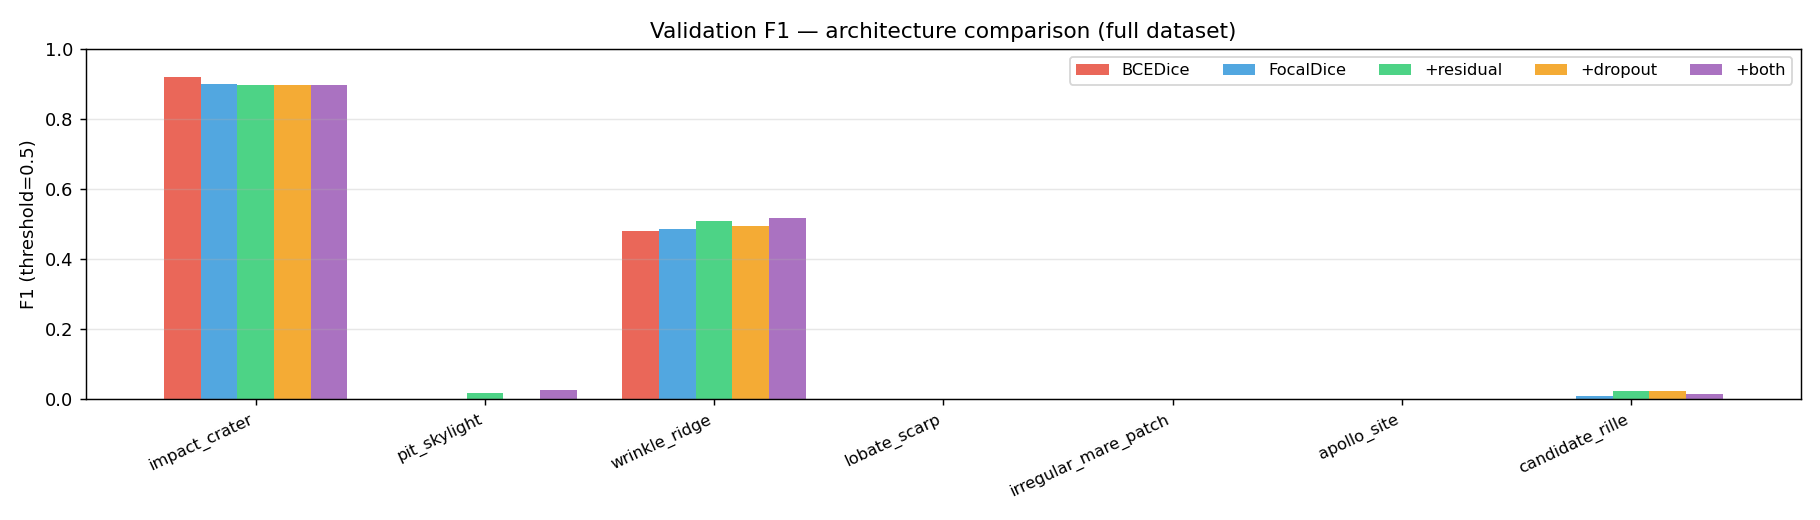
\includegraphics[width=\textwidth]{figures/MR/cloudveneto_arch_val_f1.png}
    \caption{Validation F1}
\end{subfigure}
\hfill
\begin{subfigure}[b]{0.32\textwidth}
    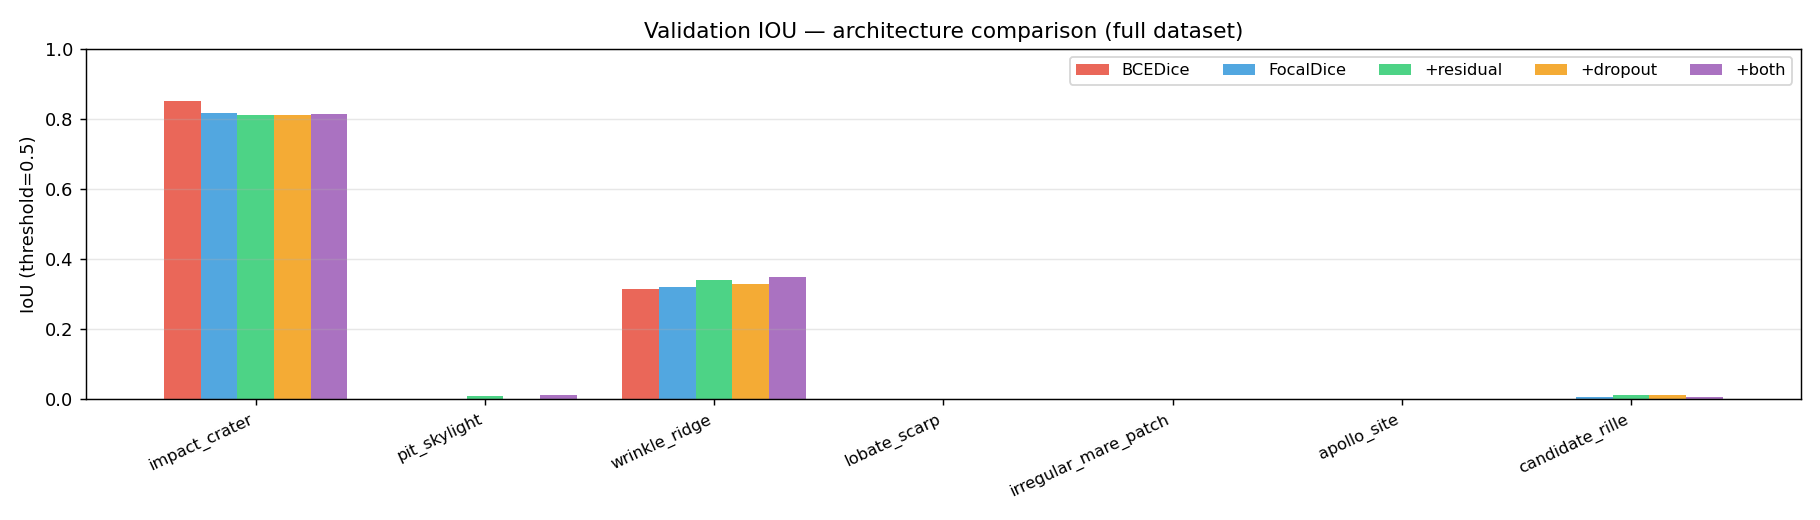
\includegraphics[width=\textwidth]{figures/MR/cloudveneto_arch_val_iou.png}
    \caption{Validation IoU}
\end{subfigure}
\hfill
\begin{subfigure}[b]{0.32\textwidth}
    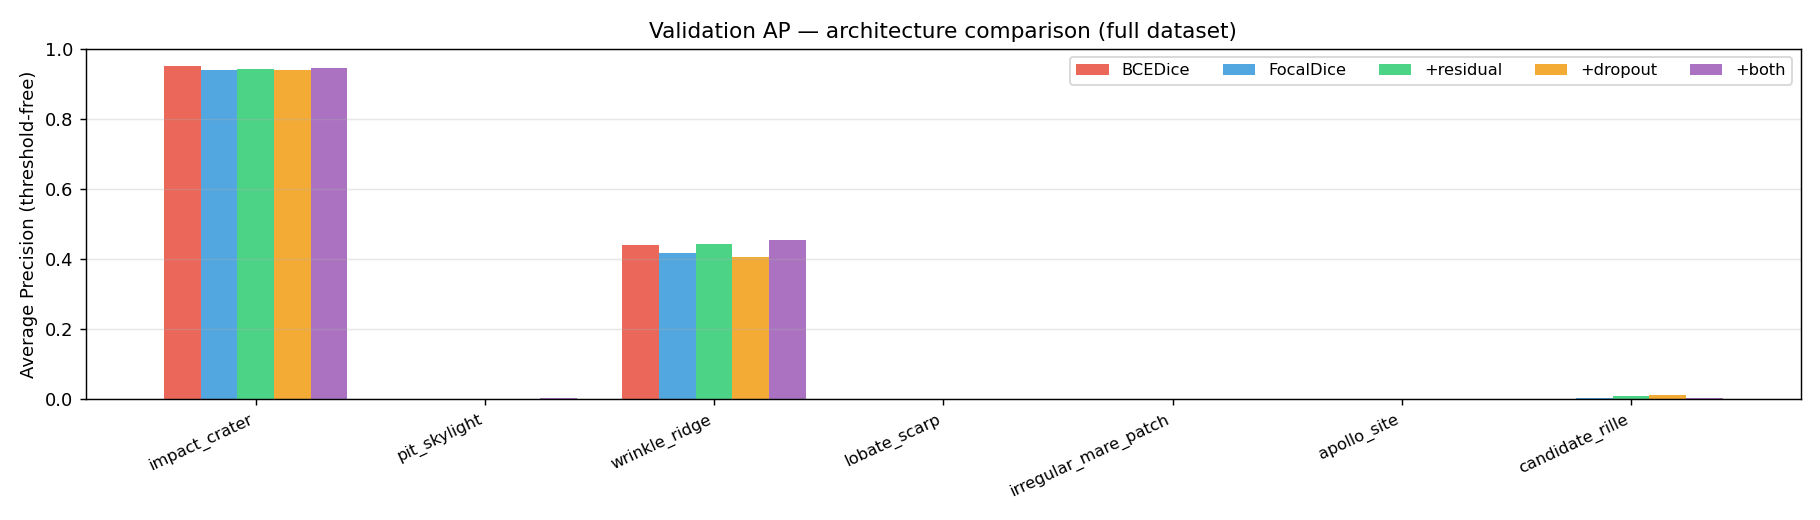
\includegraphics[width=\textwidth]{figures/MR/cloudveneto_arch_val_ap.png}
    \caption{Validation AP}
\end{subfigure}
\caption{Per-class validation metrics across training epochs for the five architecture configurations (full T4 run, 30 epochs). \textbf{+both} (residual + dropout + FocalDice) achieves the highest aggregate performance on all three metrics.}
\label{fig:arch_metrics}
\end{figure}

\paragraph{Key findings.}
Residual shortcuts consistently improve over the plain DoubleConv baseline on aggregate F1, IoU, and AP (+residual vs FocalDice: $+0.0071$ mean F1, $+0.0050$ mean AP). Dropout alone does not help — it degrades both mean AP and ridge AP relative to plain FocalDice, likely because sparse labels already act as a strong regulariser. The combination \textbf{+both} achieves the best mean F1 (0.2076), best mean IoU (0.1688), and best mean AP (0.2004), as well as the highest ridge AP (0.453). Impact-crater AP is uniformly high (0.939–0.951) across all configurations, but given the 0.821 prevalence baseline (Table~\ref{tab:prevalence}) this represents only a modest lift over chance; the architecture choice matters primarily for rare and structurally subtle classes such as ridges, where AP~0.44--0.45 is ${\sim}70\times$ the 0.0064 chance level.

% -----------------------------------------------------------------------------
\subsection{Study 2 — Network Width}
\label{sec:mr_width}

Using the best architecture from Study~1 (\textbf{+both}: FocalDice + residual + dropout=0.3), we sweep the base width $w \in \{16, 32, 64\}$, corresponding to 505K, 2.0M, and 8.0M parameters respectively.

\begin{table}[h]
\centering
\caption{Base-width sweep (FocalDice + residual + dropout=0.3, full T4 run, 30 epochs).}
\label{tab:bw_comparison}
\begin{tabular}{lrrrrrr}
\toprule
Config & Params & Epoch (s) & Mean F1 & Mean IoU & Mean AP & Ridge AP \\
\midrule
small ($w=16$)   &    505{,}095 &  139 & 0.2031 & 0.1665 & 0.2003 & 0.451 \\
default ($w=32$) & 2{,}014{,}727 &  258 & 0.2093 & 0.1704 & 0.2010 & 0.456 \\
wide ($w=64$)    & 8{,}047{,}623 &  582 & \textbf{0.2153} & \textbf{0.1733} & \textbf{0.2016} & 0.445 \\
\bottomrule
\end{tabular}
\end{table}

\begin{figure}[h]
\centering
\begin{subfigure}[b]{0.32\textwidth}
    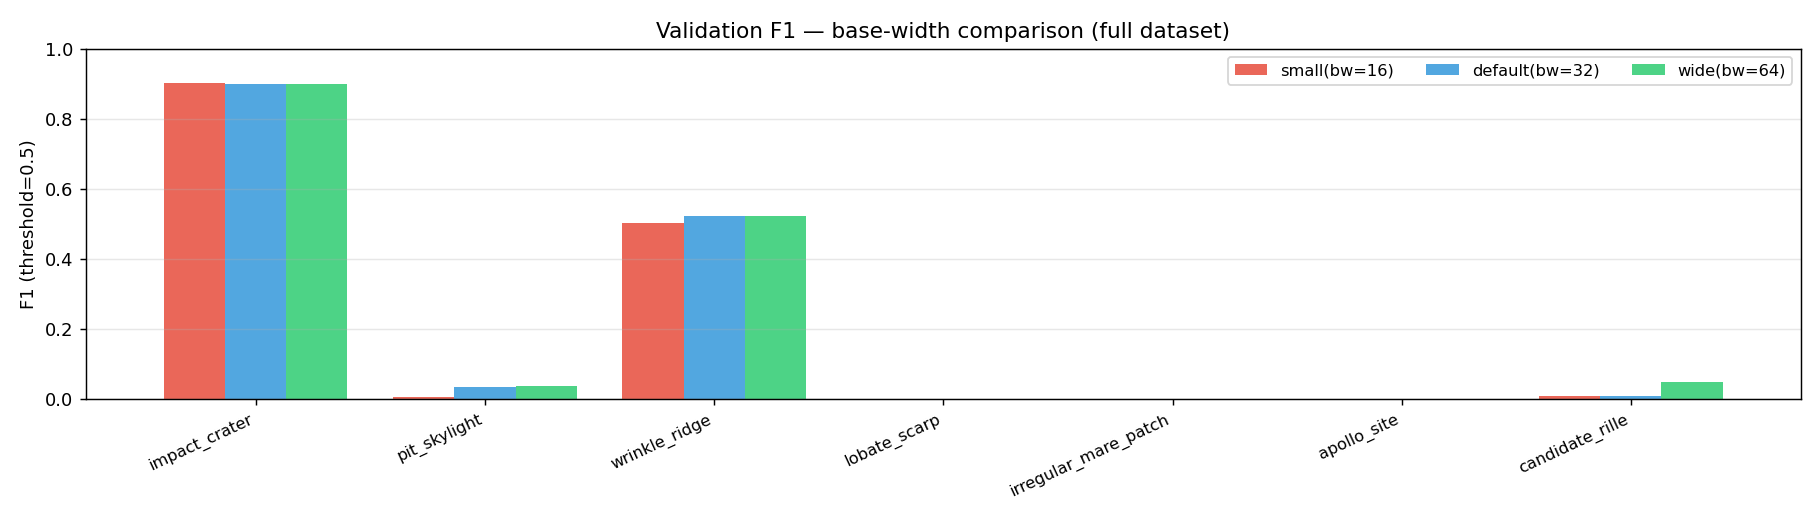
\includegraphics[width=\textwidth]{figures/MR/cloudveneto_bw_val_f1.png}
    \caption{Validation F1}
\end{subfigure}
\hfill
\begin{subfigure}[b]{0.32\textwidth}
    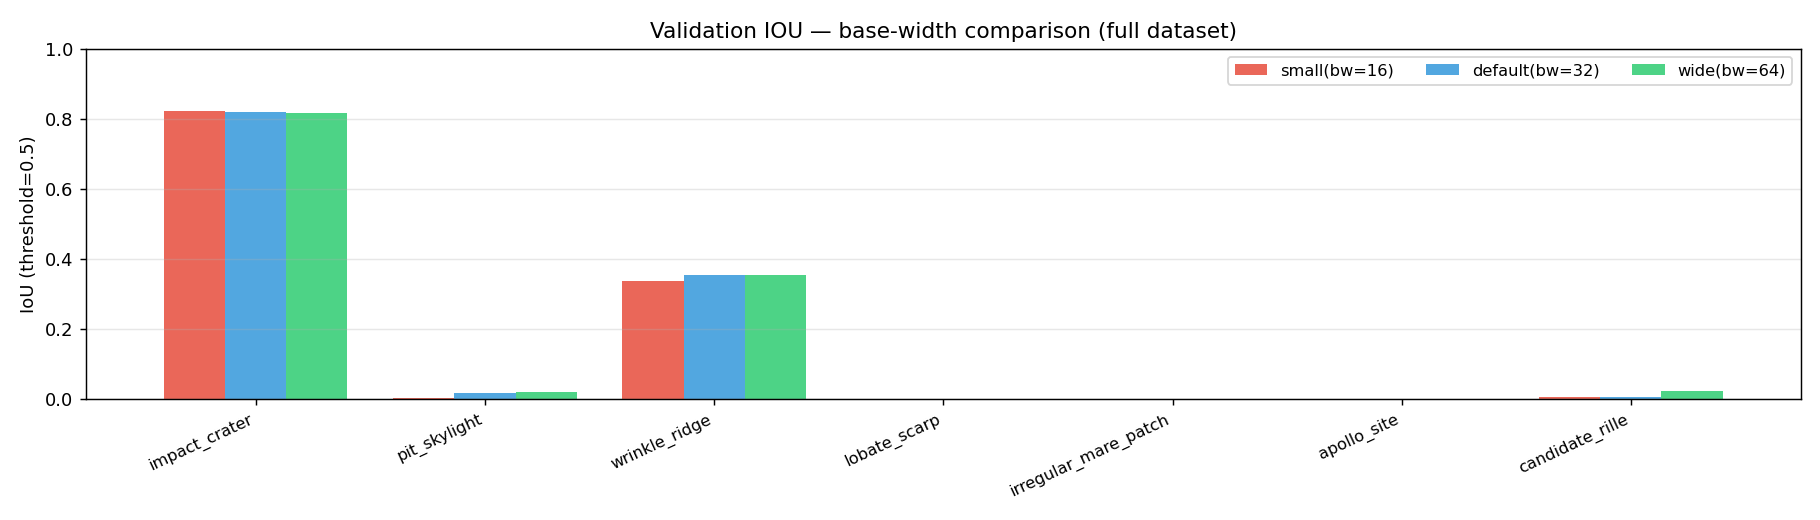
\includegraphics[width=\textwidth]{figures/MR/cloudveneto_bw_val_iou.png}
    \caption{Validation IoU}
\end{subfigure}
\hfill
\begin{subfigure}[b]{0.32\textwidth}
    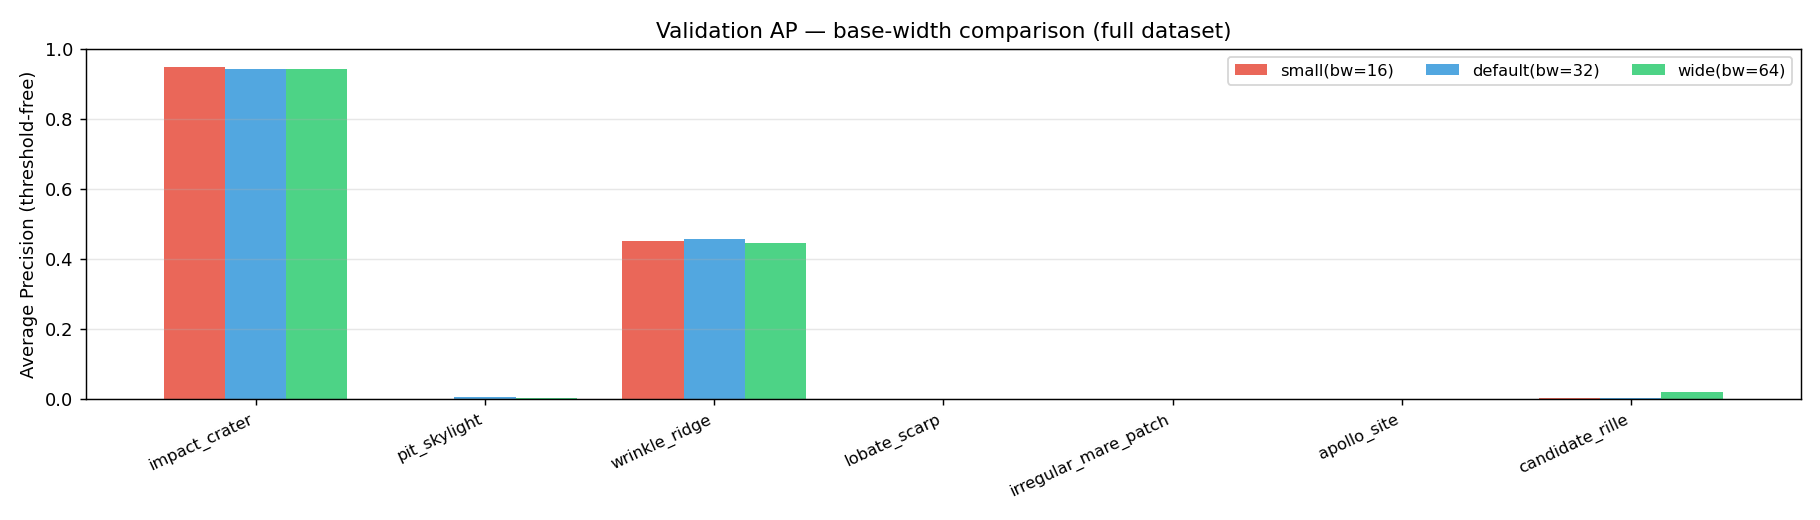
\includegraphics[width=\textwidth]{figures/MR/cloudveneto_bw_val_ap.png}
    \caption{Validation AP}
\end{subfigure}
\caption{Validation metrics for three network widths (full T4 run, 30 epochs). Wider networks achieve marginally higher scores but exhibit severely diminishing returns in terms of parameters and training time.}
\label{fig:bw_metrics}
\end{figure}

\paragraph{Key findings.}
The wide model ($w=64$) achieves the best mean AP (0.2016) and mean F1 (0.2153), but the improvement over the default ($w=32$) is marginal: $+0.0006$ mean AP, $+0.006$ mean F1, at the cost of a 4$\times$ parameter increase and a ${\sim}2.3\times$ increase in training time per epoch (258 s $\to$ 582 s). Strikingly, the small model ($w=16$) with only 505K parameters achieves a mean AP of 0.2003 — within 0.001 of the 8M-parameter wide model — making it the most parameter-efficient option. For deployment on resource-constrained hardware the small model offers the best trade-off.

% -----------------------------------------------------------------------------
\subsection{Study 3 — Data Augmentation}
\label{sec:mr_augmentation}

Using \textbf{+both} at $w=32$, we isolate the effect of geometric augmentation. The augmented pipeline applies random horizontal and vertical flips and 90°/180°/270° rotations to training tiles. No augmentation is applied to validation.

\begin{table}[h]
\centering
\caption{Augmentation study (FocalDice + residual + dropout=0.3, $w=32$, full T4 run, 30 epochs). Crater AP is given for reference; Ridge AP highlights the most affected rare class.}
\label{tab:aug_comparison}
\begin{tabular}{lrrrrrr}
\toprule
Config & Final loss & Mean F1 & Mean IoU & Mean AP & Crater AP & Ridge AP \\
\midrule
\textbf{no augmentation} & \textbf{3.698} & \textbf{0.2986} & \textbf{0.2289} & \textbf{0.2647} & \textbf{0.947} & \textbf{0.558} \\
+augmentation            &        3.863  &        0.2124  &        0.1724  &        0.2027  &        0.942  &        0.457  \\
\bottomrule
\end{tabular}
\end{table}

\begin{figure}[h]
\centering
\begin{subfigure}[b]{0.32\textwidth}
    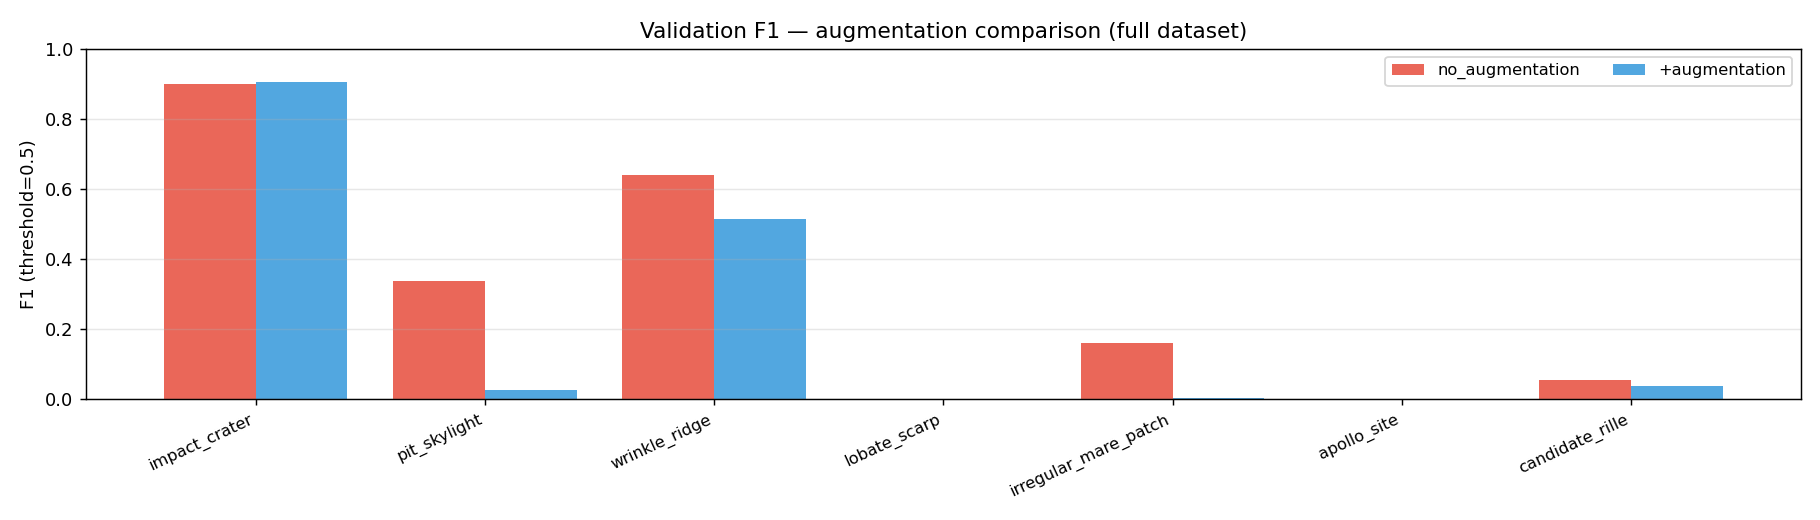
\includegraphics[width=\textwidth]{figures/MR/cloudveneto_aug_val_f1.png}
    \caption{Validation F1}
\end{subfigure}
\hfill
\begin{subfigure}[b]{0.32\textwidth}
    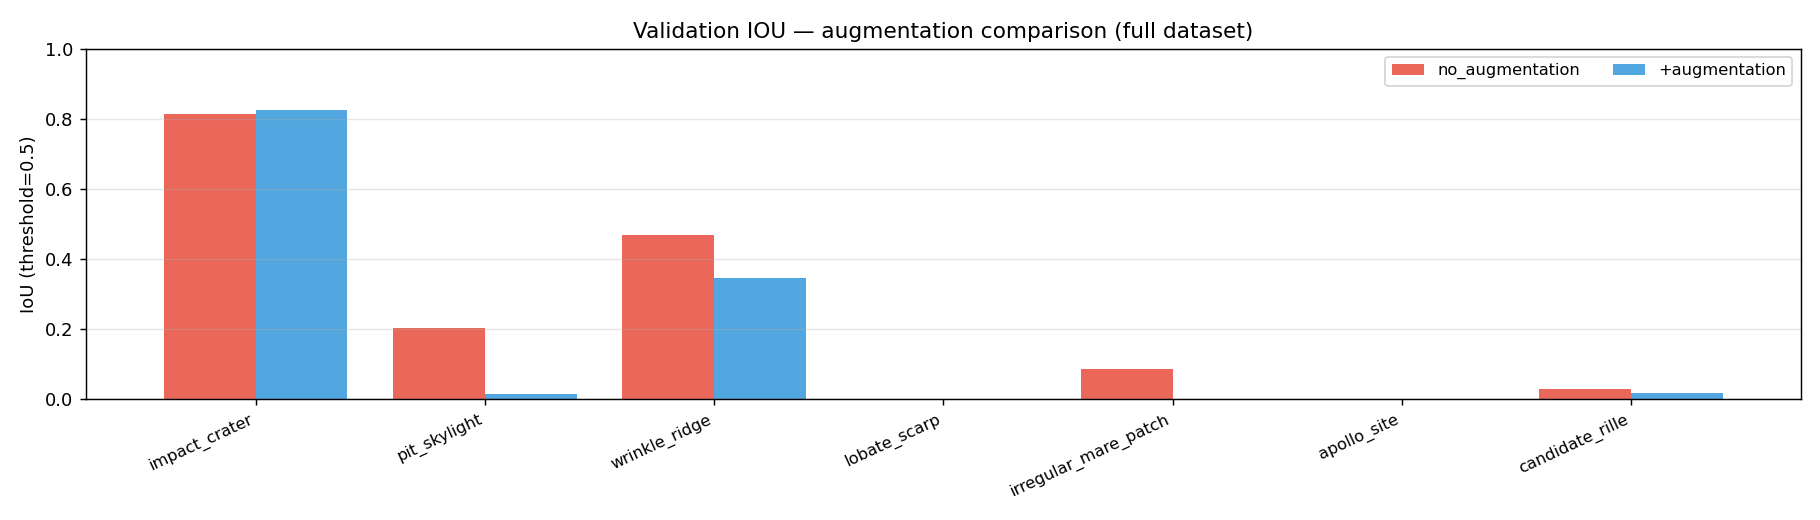
\includegraphics[width=\textwidth]{figures/MR/cloudveneto_aug_val_iou.png}
    \caption{Validation IoU}
\end{subfigure}
\hfill
\begin{subfigure}[b]{0.32\textwidth}
    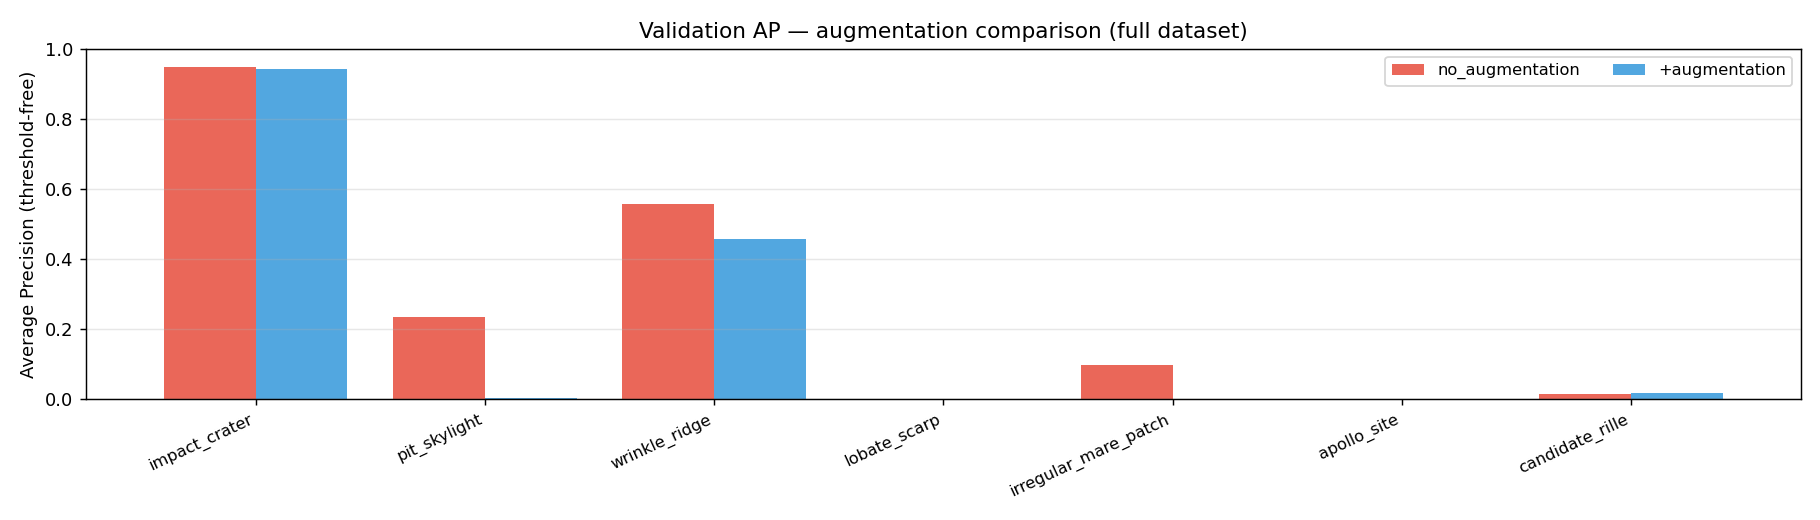
\includegraphics[width=\textwidth]{figures/MR/cloudveneto_aug_val_ap.png}
    \caption{Validation AP}
\end{subfigure}
\caption{Validation metrics with and without geometric augmentation (full T4 run, 30 epochs). No augmentation outperforms the augmented training on all metrics.}
\label{fig:aug_metrics}
\end{figure}

\paragraph{Key findings.}
This is the most striking result of the ablation campaign. Training without augmentation produces a model that is dramatically better on every metric: mean F1 improves by 0.086 (40\% relative), mean AP improves by 0.062 (31\% relative), and ridge AP improves from 0.457 to 0.558 (22\% relative).

Two effects plausibly combine to produce this result, and the present experiment cannot fully separate them.

First, a \emph{geological} effect: the Marius Hills region has a strong directional bias — wrinkle ridges run predominantly in a narrow range of orientations dictated by the regional stress field, and rilles follow the same orientation. Moreover, the Sun azimuth is consistent within the WAC mosaic, so flips and $90°$ rotations also produce illumination directions that never occur in the data. Applying such transforms presents the model with feature orientations and shading that are physically absent in the training region, injecting false diversity. Generic augmentation implicitly assumes that the transformed inputs remain representative of the target distribution~\cite{shorten2019augmentation}, an assumption violated here — the course material itself cautions against ``arbitrary rotations if illumination direction carries physical meaning''~\cite{zingales2026lecture}. Impact craters, being rotationally symmetric, are unaffected, which explains why crater AP is nearly identical in both conditions (0.947 vs 0.942).

Second, a \emph{methodological} confound: as noted in Sec.~\ref{sec:mr_dataset}, the random tile split leaks overlapping pixels into validation. A model trained without augmentation is freer to memorise tile appearance and is rewarded for it on a leaky split, while augmentation suppresses exactly this memorisation. Part of the measured gap could therefore be an artefact of the split rather than a property of the data. To separate the two effects, the comparison was re-run under the leakage-free spatial block split.

\paragraph{Leakage-free re-run.}
The augmentation pair was re-trained with \texttt{spatial\_train\_val\_split}: both arms share an identical pixel-disjoint split, the same initialisation seed, and the same cosine schedule, so the \emph{only} difference between them is augmentation. The re-run used a scaled paired protocol on local hardware (10{,}000 tiles, 30 epochs; a paired comparison remains internally valid at reduced scale), with a smaller 6{,}000-tile/15-epoch run giving consistent results. Table~\ref{tab:spatial_rerun} and Figure~\ref{fig:spatial_rerun} report the outcome.

\begin{table}[h]
\centering
\caption{Augmentation ablation under the leakage-free spatial split (10{,}000 tiles, 30 epochs, paired arms). \texttt{candidate\_rille} has zero positive pixels in the spatial validation set and is excluded from the macro averages (reported as NaN with zero support).}
\label{tab:spatial_rerun}
\begin{tabular}{lrrrr}
\toprule
Config & Mean F1 & Mean AP & Ridge F1 & Ridge AP \\
\midrule
\textbf{no augmentation} & \textbf{0.2294} & \textbf{0.2239} & \textbf{0.4586} & \textbf{0.3847} \\
+augmentation            &        0.2208  &        0.2096  &        0.3970  &        0.3060  \\
\bottomrule
\end{tabular}
\end{table}

\begin{figure}[h]
\centering
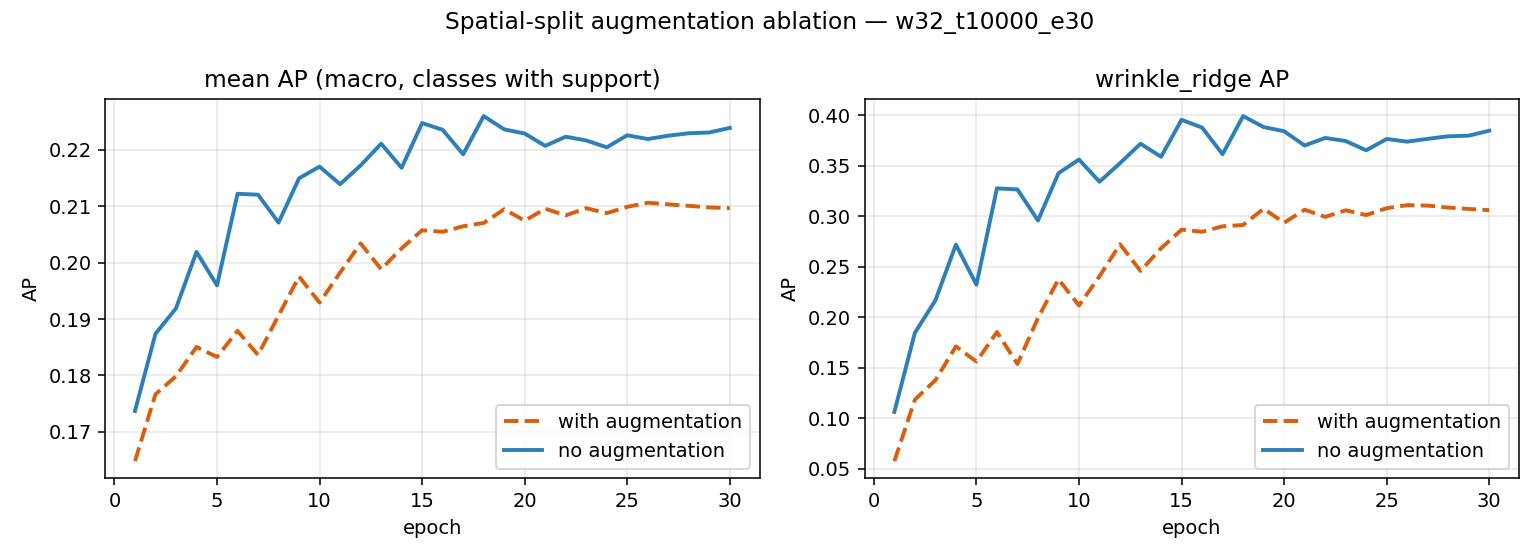
\includegraphics[width=\textwidth]{figures/MR/spatial_w32_t10000_e30_val_ap.png}
\caption{Validation AP across training epochs under the spatial split (macro mean over classes with support, left; \texttt{wrinkle\_ridge}, right). The no-augmentation arm dominates at every epoch on both metrics.}
\label{fig:spatial_rerun}
\end{figure}

The re-run \textbf{confirms the conclusion}: training without augmentation remains better, with the no-augmentation arm above the augmented one at every epoch (Fig.~\ref{fig:spatial_rerun}). The decomposition is, however, instructive. Absolute scores are substantially lower than on the leaky split (ridge AP 0.385 vs 0.558), confirming that random-split numbers were inflated by memorisation. The \emph{aggregate} advantage of no-augmentation also narrows (mean AP $+0.014$ here vs $+0.062$ on the leaky split), showing that part of the originally measured gap was indeed a split artefact. But for the direction-sensitive class the gap persists and is large — ridge AP 0.385 vs 0.306, a 26\% relative difference on strictly disjoint validation pixels — which is precisely the signature predicted by the geological explanation: augmentation hurts where orientation and illumination carry physical information. Confirmation at the full 15{,}931-tile T4 protocol remains scheduled, but the conclusion no longer rests on a confounded measurement.

% -----------------------------------------------------------------------------
\subsection{Qualitative Evaluation}
\label{sec:mr_qualitative}

Segmentation metrics alone do not reveal \emph{how} a model fails, so we complement the ablations with a visual comparison on identical validation tiles: raw image, ground truth, predicted probability, and a true-positive/false-positive/false-negative decomposition at threshold $0.5$, for the BCEDice baseline and the definitive model side by side (generated by \texttt{scripts/qualitative\_eval.py}; tiles are the three validation tiles with the largest \texttt{wrinkle\_ridge} ground-truth area).

\begin{figure}[h]
\centering
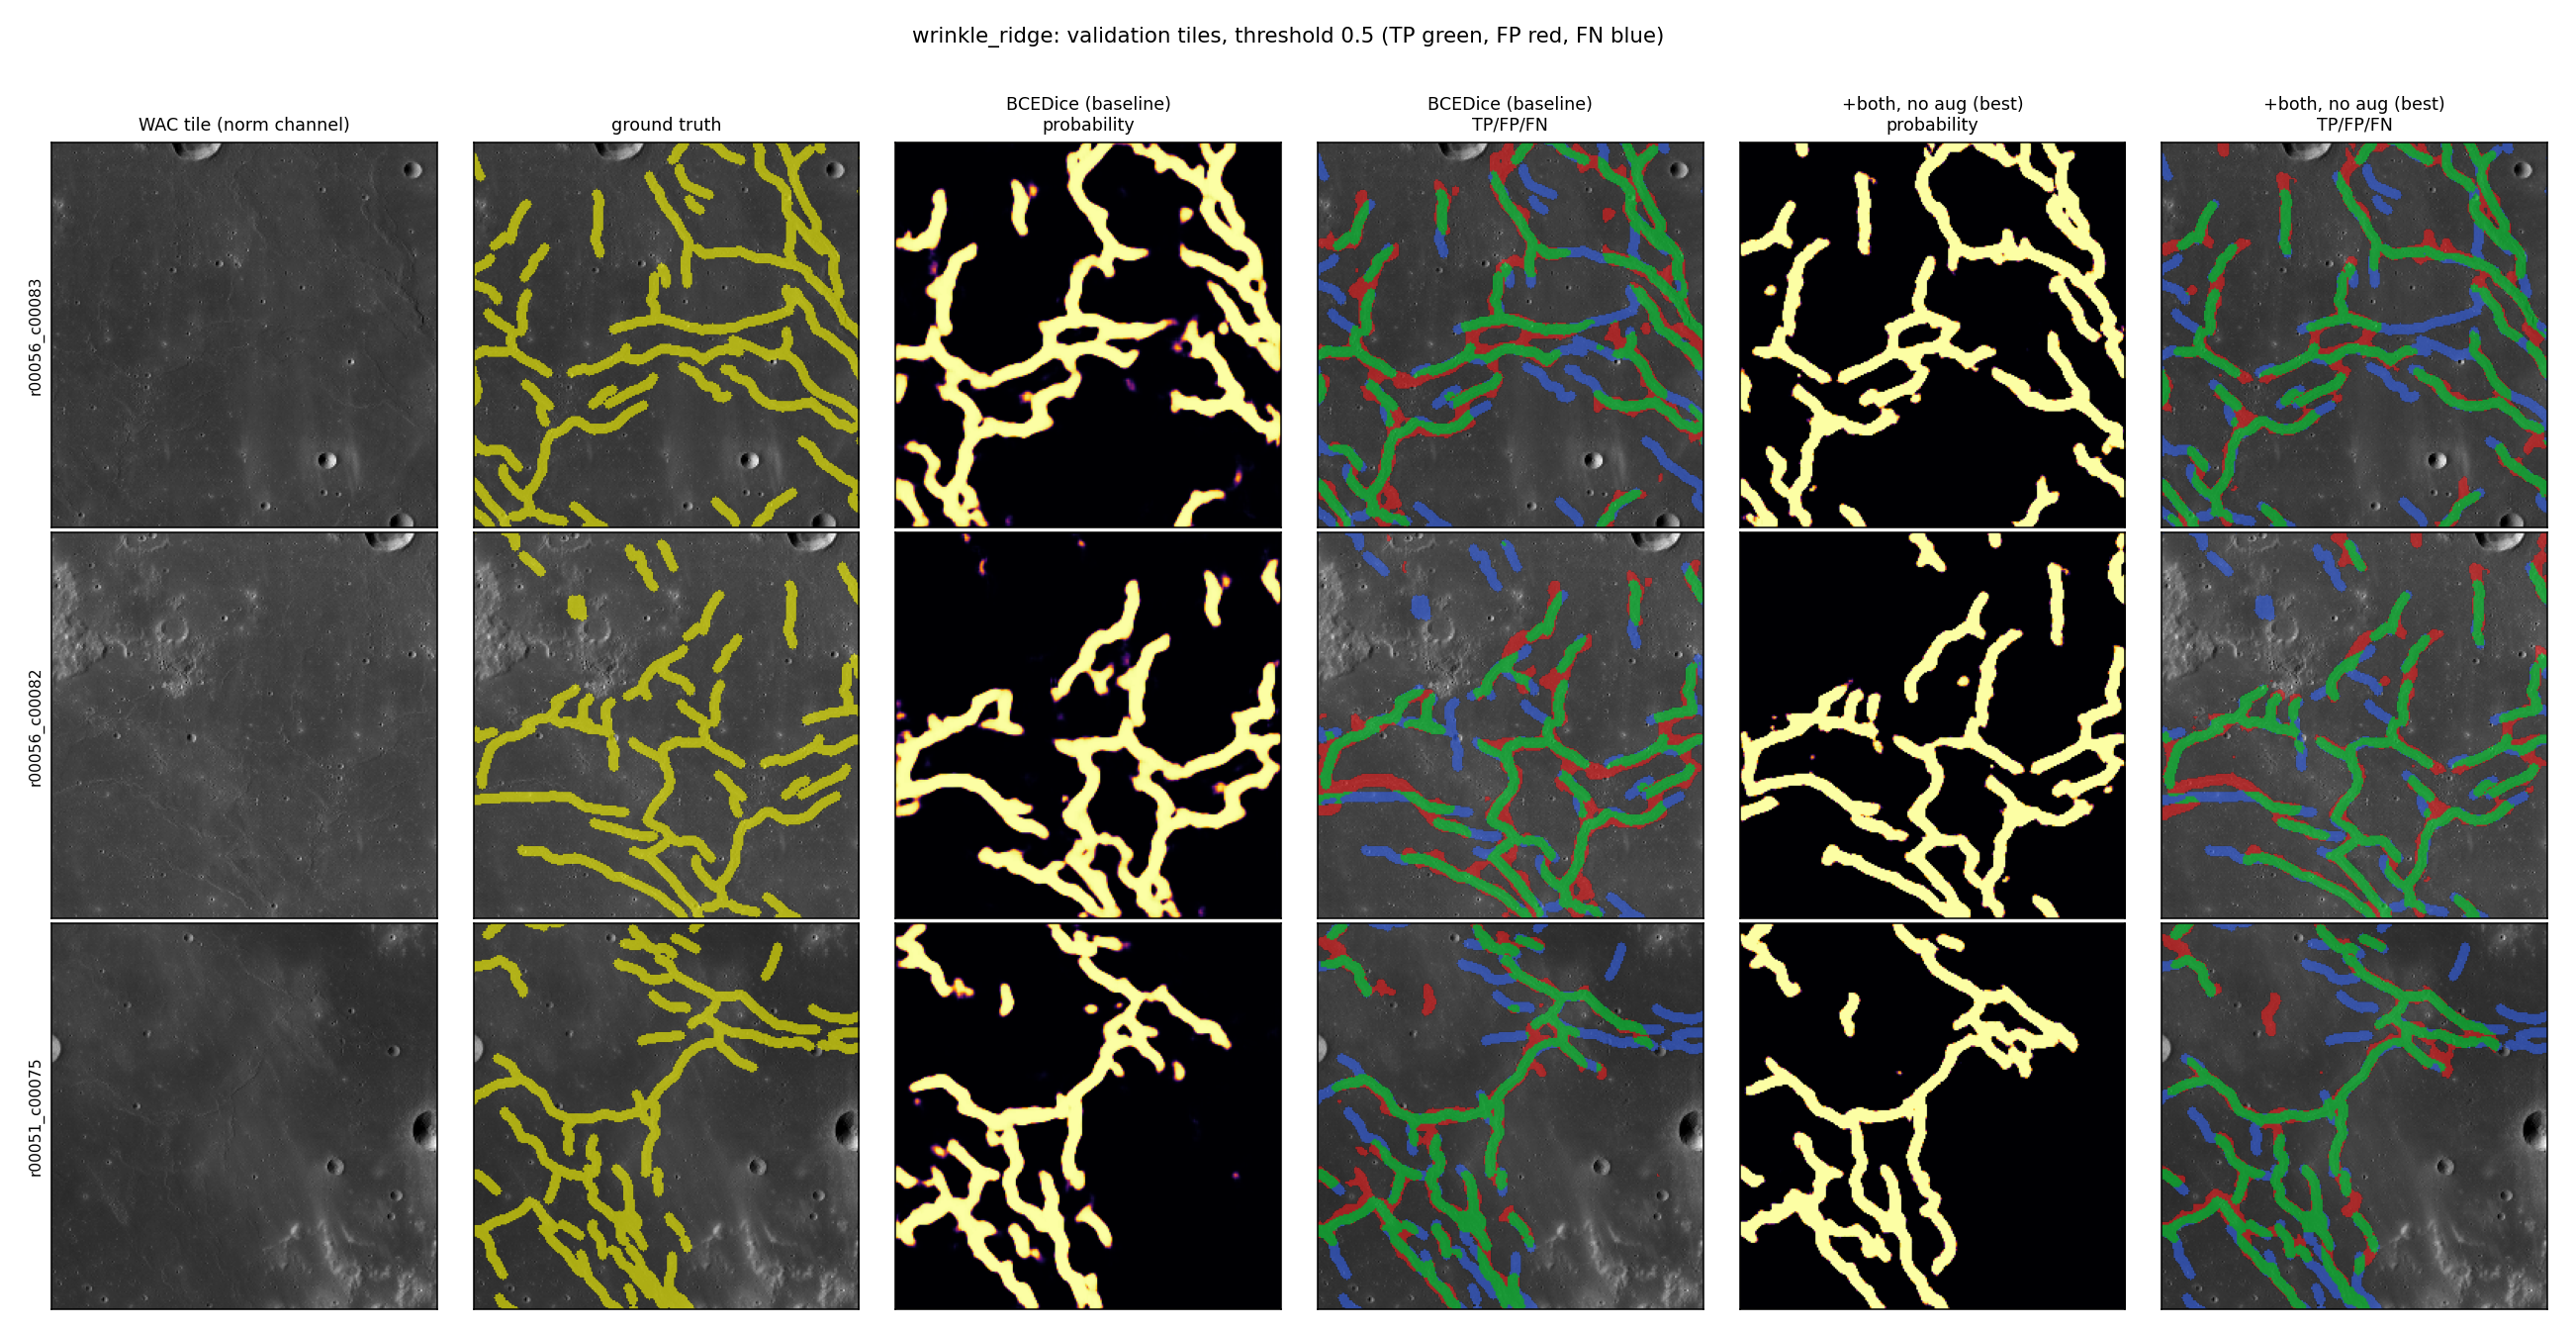
\includegraphics[width=\textwidth]{figures/MR/qualitative_wrinkle_ridge.png}
\caption{Wrinkle-ridge qualitative comparison on three validation tiles (TP green, FP red, FN blue). Both models recover the topology of the ridge network; the definitive model (+both, no augmentation) produces visibly more complete coverage and fewer false positives than the BCEDice baseline. Errors concentrate on thin, low-contrast ridge segments, consistent with the localisation difficulty of linear features.}
\label{fig:qualitative_ridge}
\end{figure}

\begin{figure}[h]
\centering
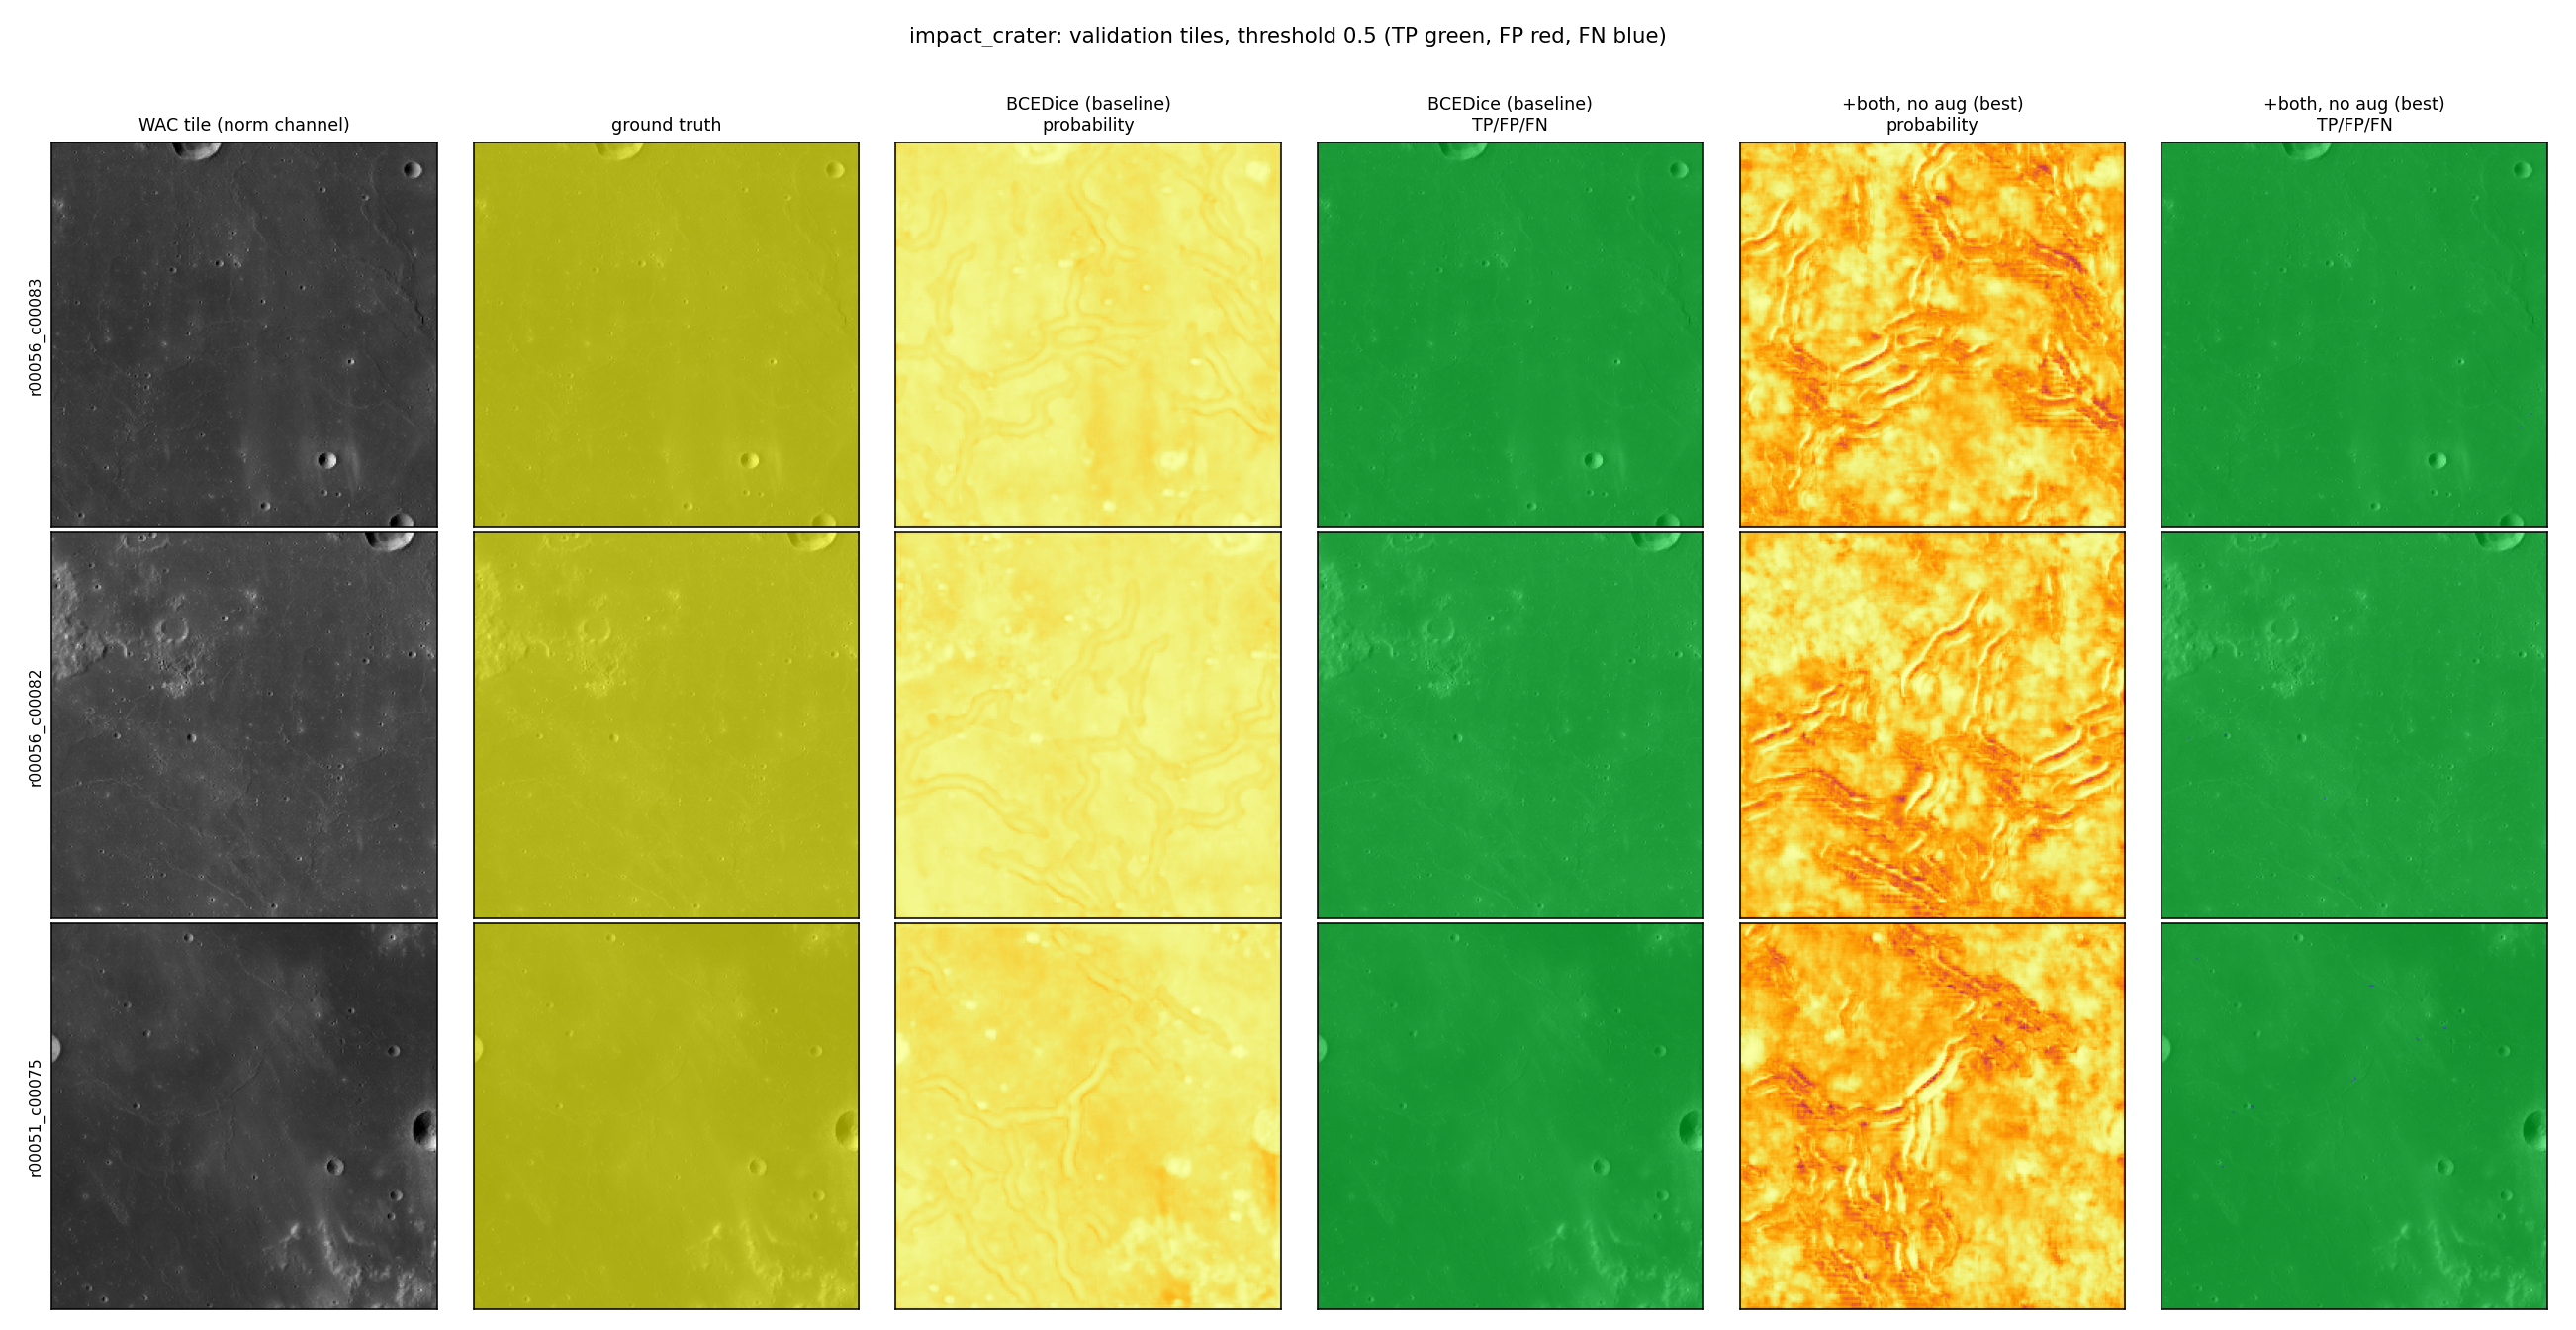
\includegraphics[width=\textwidth]{figures/MR/qualitative_impact_crater.png}
\caption{Impact-crater qualitative comparison on the same tiles. The ground truth covers the \emph{entire} tile (cf.\ the 82\% prevalence and 50.7\% fully-covered tiles of Table~\ref{tab:prevalence}), so a prediction of ``everywhere'' is trivially correct: this figure is direct visual evidence that the crater channel behaves as a near-coverage layer and that crater AP must be read against its 0.821 chance baseline.}
\label{fig:qualitative_crater}
\end{figure}

The ridge comparison shows that the metric gains of the definitive model correspond to a real, visible improvement in completeness of the recovered ridge network. The crater comparison, conversely, makes the saturation argument of Sec.~\ref{sec:mr_dataset} concrete.

% -----------------------------------------------------------------------------
\subsection{South Pole Inference}
\label{sec:mr_south_pole}

The best-performing model weights (\texttt{best\_trained.pth}) were applied to the lunar south pole to demonstrate transfer beyond the training region. The south pole imagery was obtained from the same LRO WAC source and tiled identically, producing 3{,}639 tiles.

\paragraph{Inference pipeline.}
Each tile is preprocessed with the same CLAHE + Sobel three-channel pipeline. A sliding-window predictor runs the model tile by tile, saving per-class probability maps as compressed \texttt{.npz} files for downstream aggregation. Probability maps are aggregated over all tiles to compute global statistics.

\paragraph{Per-class results.}
Table~\ref{tab:south_pole_stats} reports the aggregated statistics over the 3{,}639 south pole tiles.

\begin{table}[h]
\centering
\caption{South pole inference results (3{,}639 tiles). Avg.\ Max.\ Prob.\ is the mean, over tiles, of the maximum predicted probability for each class. Global Max is the highest probability observed in any single tile. A high avg.\ max but low global max indicates diffuse, uncertain detections; a high global max but low avg.\ max indicates rare but confident detections.}
\label{tab:south_pole_stats}
\begin{tabular}{lrrr}
\toprule
Class & Avg.\ Max.\ Prob. & Global Max & Status \\
\midrule
\texttt{impact\_crater}       & 0.863 & 1.000 & \checkmark\ detected \\
\texttt{lobate\_scarp}        & 0.060 & 0.303 & weak \\
\texttt{pit\_skylight}        & 0.051 & 0.202 & weak \\
\texttt{irregular\_mare\_patch} & 0.040 & 0.215 & weak \\
\texttt{apollo\_site}         & 0.040 & 0.183 & weak \\
\texttt{candidate\_rille}     & 0.006 & 0.480 & sparse \\
\texttt{wrinkle\_ridge}       & 0.001 & 1.000 & sparse \\
\bottomrule
\end{tabular}
\end{table}

\begin{figure}[h]
\centering
\begin{subfigure}[b]{0.48\textwidth}
    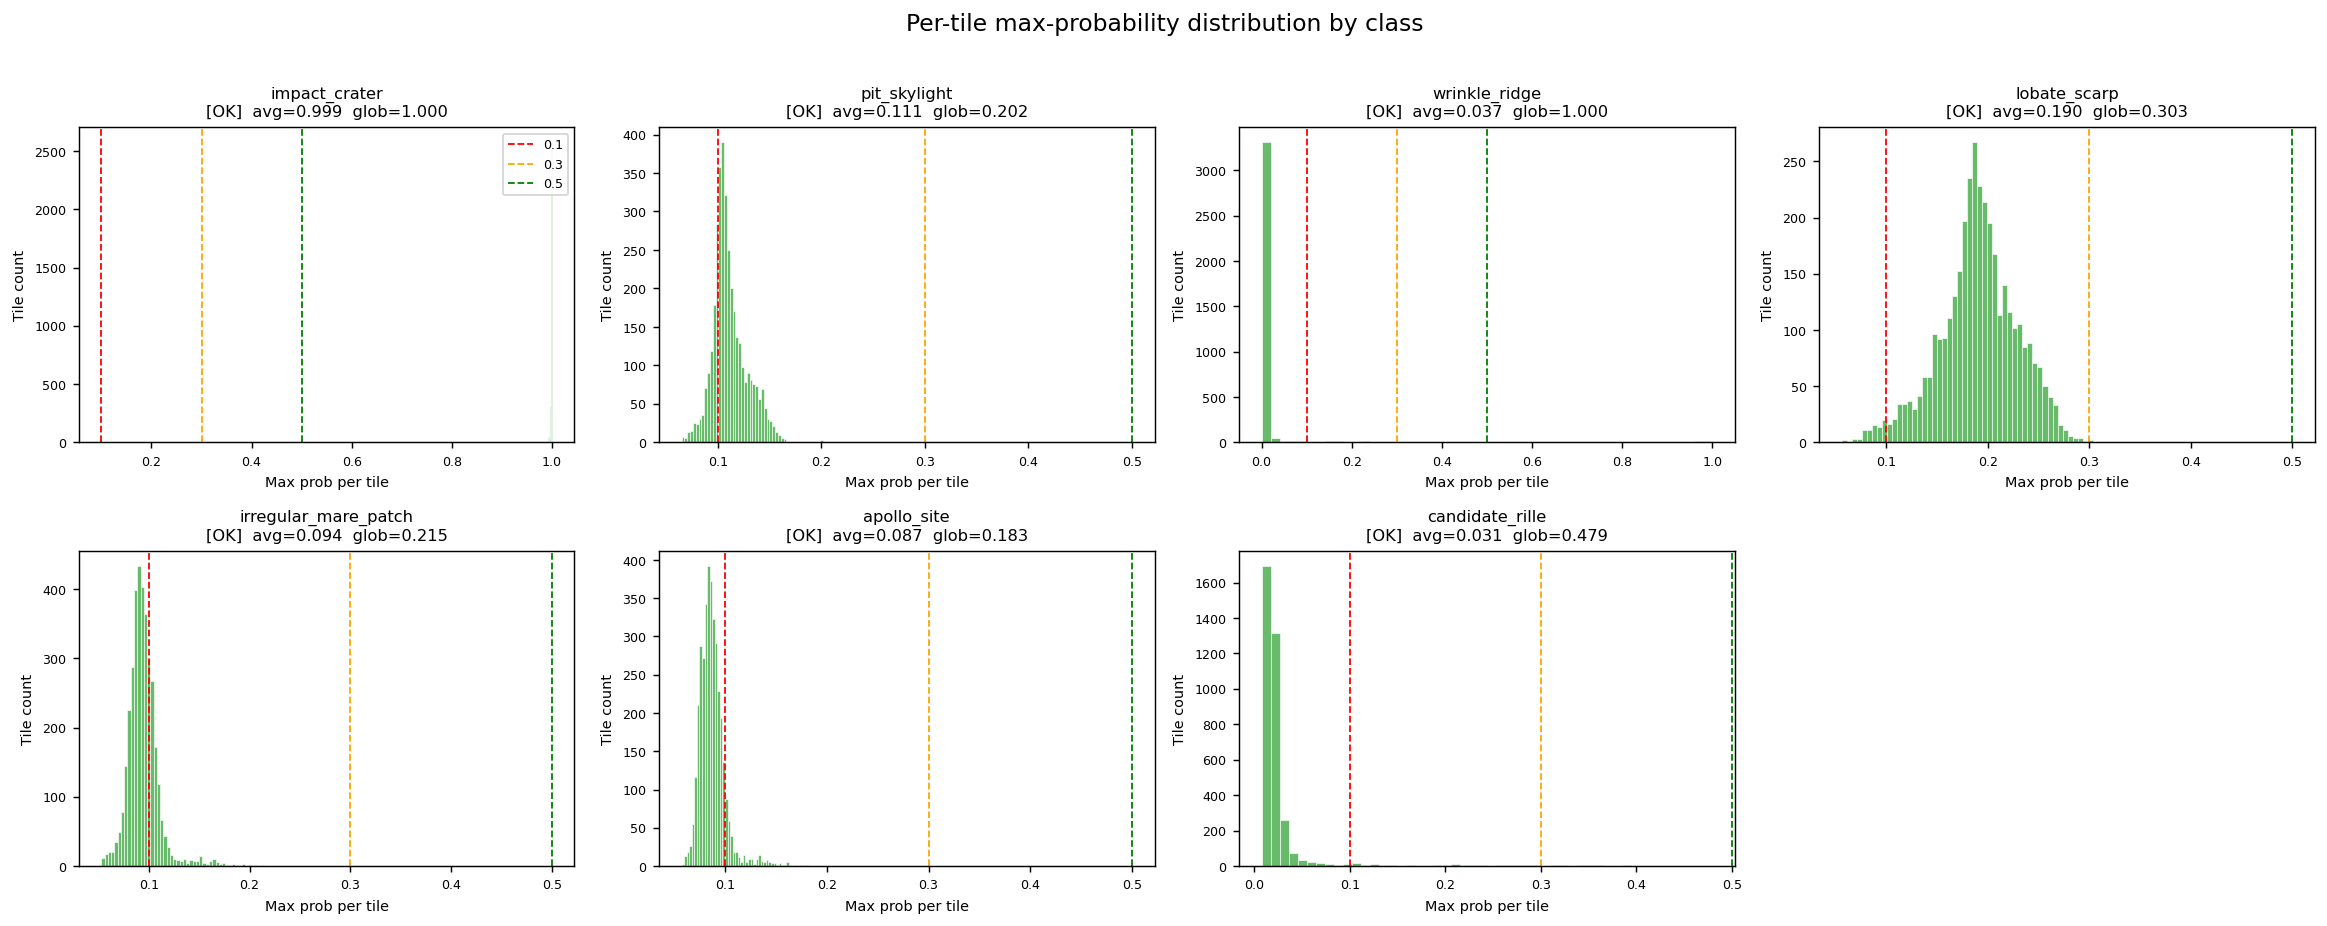
\includegraphics[width=\textwidth]{figures/MR/diagnostics_distributions.png}
    \caption{Per-tile max-probability distributions.}
\end{subfigure}
\hfill
\begin{subfigure}[b]{0.48\textwidth}
    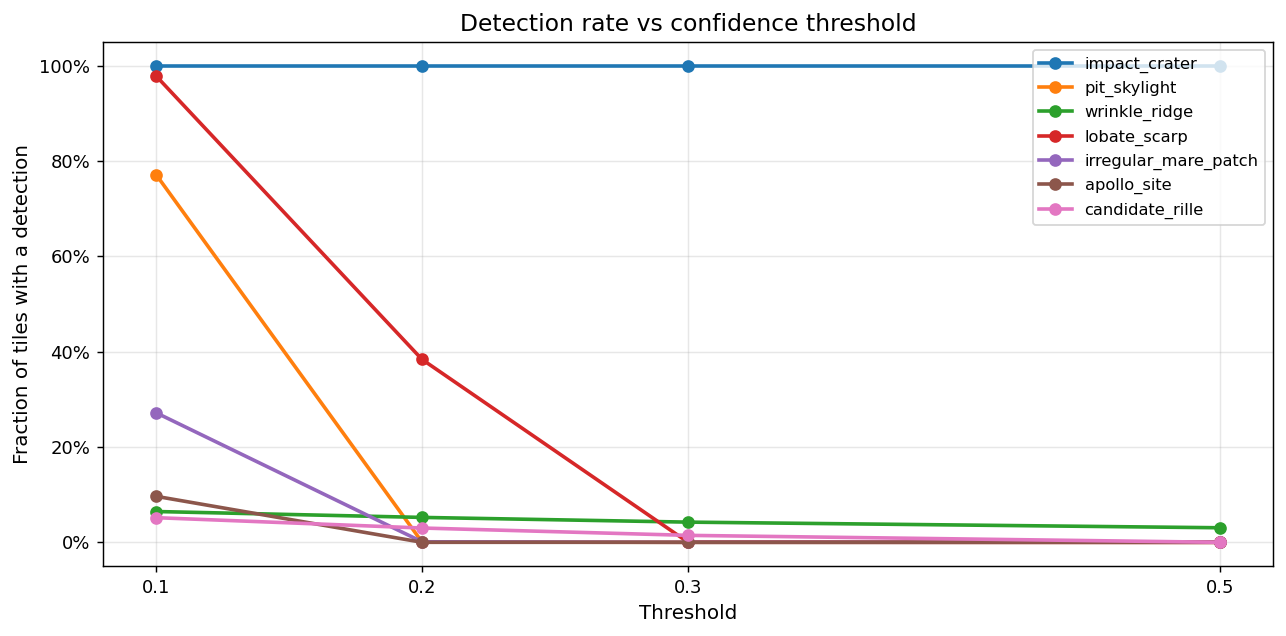
\includegraphics[width=\textwidth]{figures/MR/diagnostics_detection_rates.png}
    \caption{Detection rate vs.\ confidence threshold.}
\end{subfigure}
\caption{South pole inference diagnostics across 3{,}639 tiles. Impact craters are detected with near-certainty across the entire region. All other classes exhibit strongly right-skewed distributions with low average confidence, reflecting both the domain shift from Marius Hills and the scarcity of these features at the south pole.}
\label{fig:south_pole_diag}
\end{figure}

\begin{figure}[h]
\centering
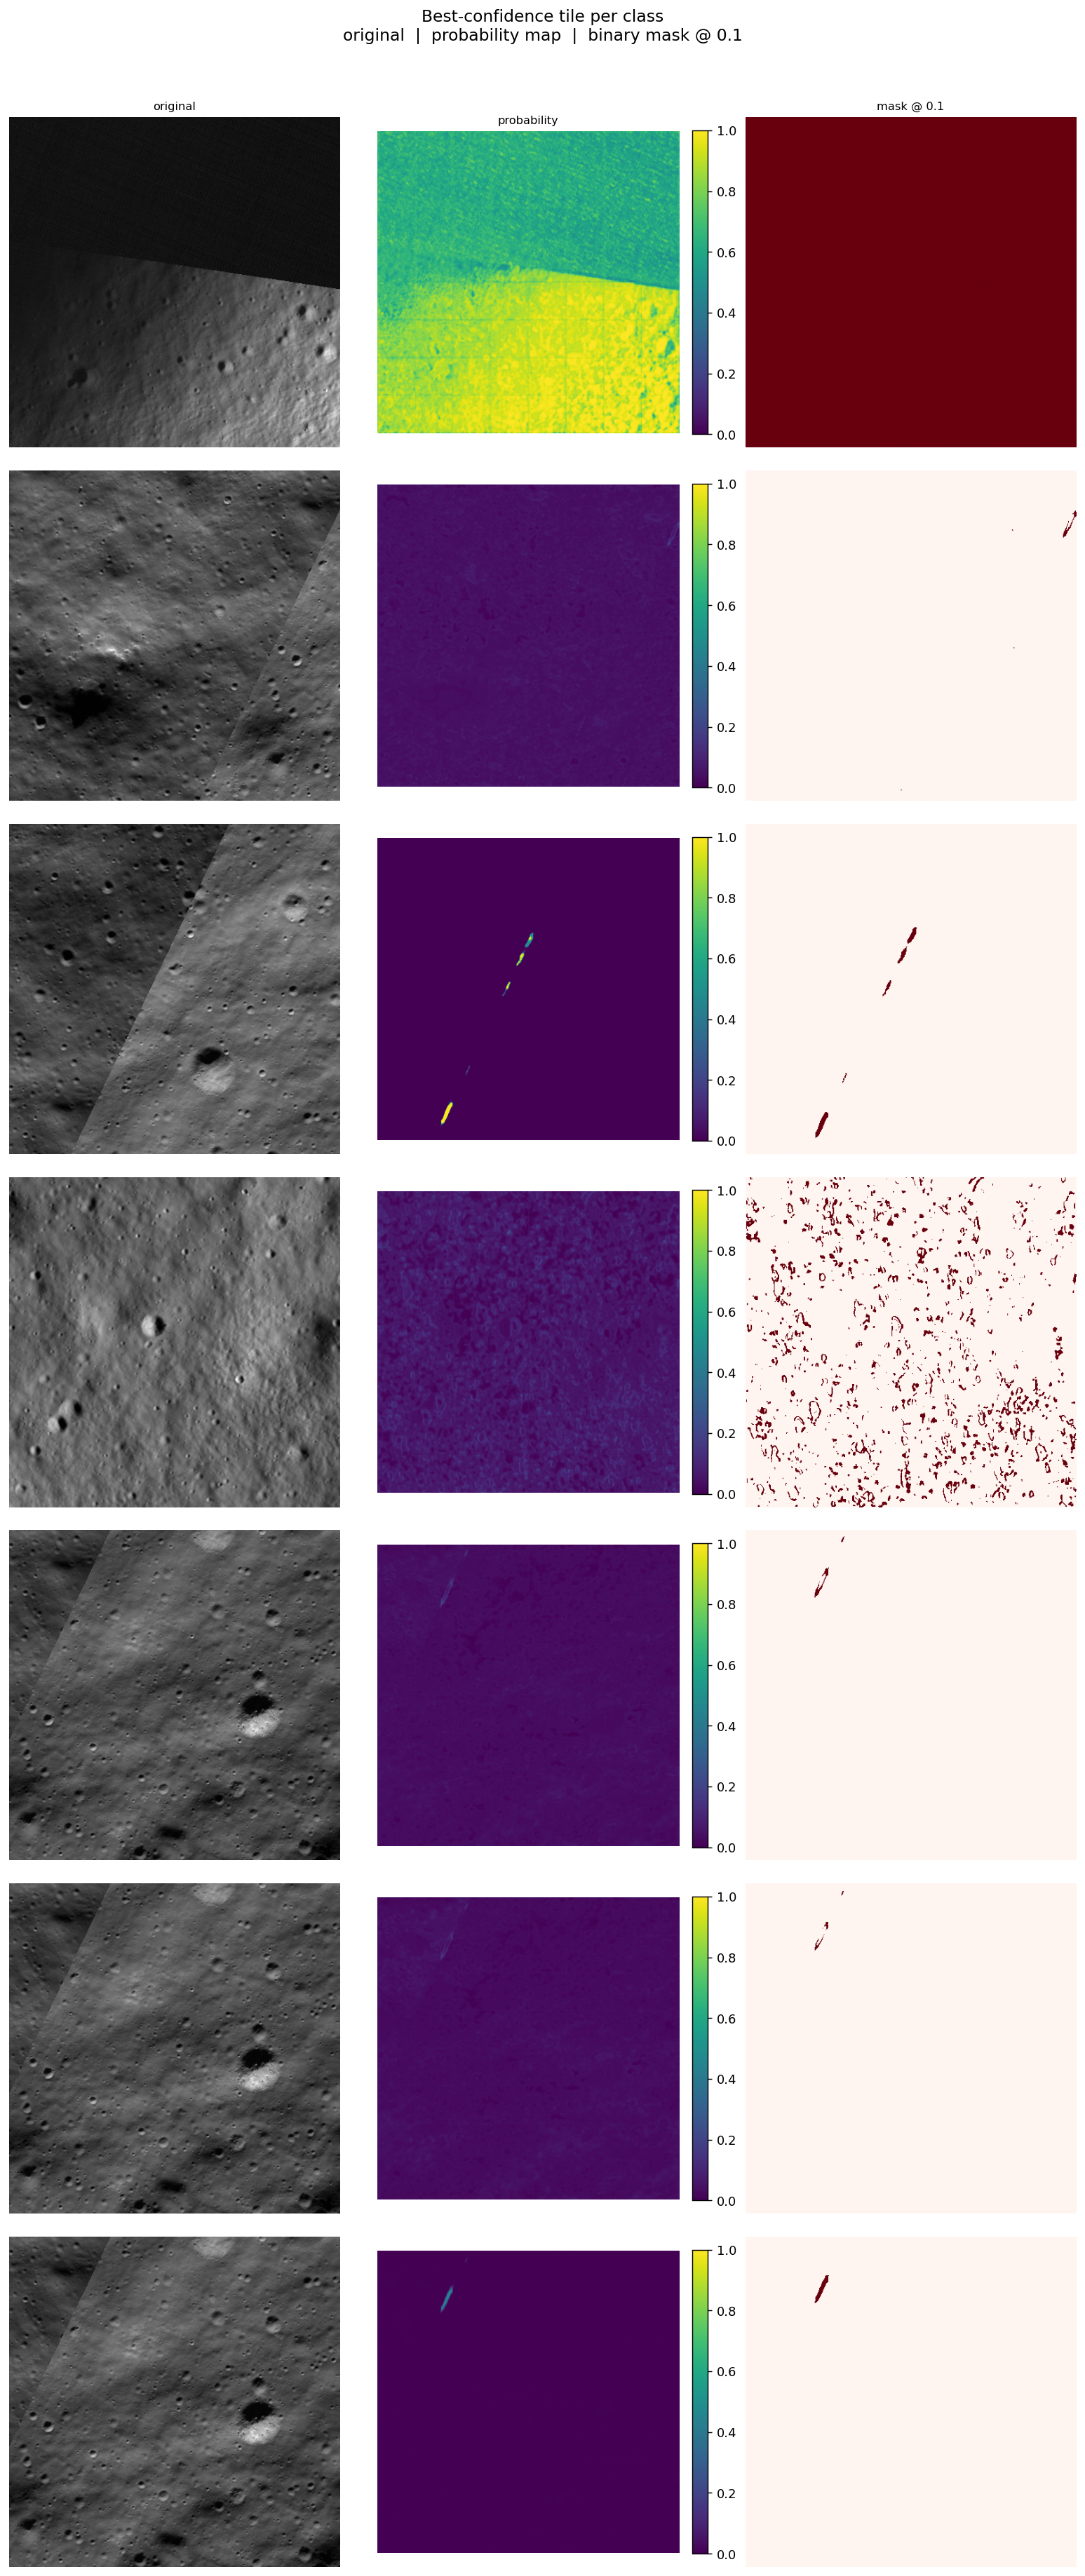
\includegraphics[width=\textwidth, height=0.82\textheight, keepaspectratio]{figures/MR/diagnostics_best_tiles.png}
\caption{Best-detected tile per class on the south pole imagery. Each panel shows the LRO WAC tile overlaid with the predicted probability map for the class with the highest maximum confidence in that tile. Note that overlays use a \emph{relative} threshold (top fraction of each tile's probabilities) so that the most likely candidate pixels are visible even when absolute confidence is low; coloured regions for the weak classes are therefore candidate locations, not confident detections. Impact craters stand out clearly; other classes show localised but low-confidence activations.}
\label{fig:south_pole_best}
\end{figure}

\paragraph{Analysis.}
The model assigns high crater probability across the entire south pole (average max probability 0.863). Given the near-saturated crater layer learned in training (Sec.~\ref{sec:mr_dataset}), this is expected behaviour — the model has learned that almost everywhere is ``crater'' — and should not be over-interpreted as precise crater delineation. Two classes — \texttt{wrinkle\_ridge} and \texttt{candidate\_rille} — show an interesting pattern: very low average-tile probabilities (0.001 and 0.006) but anomalously high global maxima (1.000 and 0.480). This indicates that the model makes rare but high-confidence predictions on a small number of tiles, rather than diffuse low-confidence activations everywhere.

The weak performance on rare classes at the south pole is attributable to two combined factors. First, the south pole is geologically distinct from Marius Hills: it lacks the volcanic structures (skylights, rilles, ridges) that dominate the training distribution, making it an out-of-distribution region for those classes. Second, the extremely low frequency of those classes in the training data means the model has seen very few positive examples even during Marius Hills training. Both issues motivate future work on label-efficient transfer learning and domain adaptation.

% -----------------------------------------------------------------------------
\subsection{Methodological Audit and Reproducibility}
\label{sec:mr_audit}

After the experimental campaign was completed, the entire pipeline — code, data, report claims, and course guidance — was subjected to a systematic audit. Every resulting change is a single, individually justified commit on the \texttt{U-net} branch, indexed in \texttt{Moon-Recognition/IMPROVEMENTS.md}; the executed notebooks were committed \emph{before} any fix, so the provenance of the published numbers is preserved. This section summarises what the audit found and how each finding affects the interpretation of the results — both as a record for the group and because several findings changed the conclusions of this report.

\paragraph{(a) Report--code reconciliation.}
Several statements in an earlier draft did not match the implementation and were corrected against the code as ground truth: the CLAHE parameters (the pipeline uses \texttt{skimage} \texttt{equalize\_adapthist} with clip limit 0.03, not the OpenCV-style values previously quoted), the tiling description (tiles \emph{overlap} by 50\%), the split procedure (random permutation, not sequential), a gradient-clipping claim (clipping was never enabled), and a mis-attributed citation in the augmentation discussion (replaced with the correct survey~\cite{shorten2019augmentation}). The principle applied: any claim an examiner can check against the repository must be checkable.

\paragraph{(b) Train/validation leakage --- discovery and remedy.}
Because adjacent tiles share 50\% of their pixels, the random tile-level split leaks: a direct measurement on the real index showed that \textbf{100\% of the 3{,}186 validation tiles overlap at least one training tile}. This inflates absolute validation scores and specifically confounds the augmentation study, since a non-augmented model is freer to memorise tile appearance and a leaky validation set rewards exactly that memorisation. The remedy, recommended by the course material itself, is a \emph{spatial block split}: contiguous $1024$-px blocks are assigned to validation and every training tile whose footprint intersects a validation tile is discarded ($\texttt{data/splits.py}$; on the real index: 11{,}289 train / 3{,}248 validation tiles, 1{,}394 boundary tiles dropped, zero pixel overlap, verified by an independent assertion). The augmentation comparison was re-run under this split as a scaled paired protocol on local hardware (both arms share an identical split, initialisation, and schedule, so the comparison is internally valid); the conclusion was confirmed, with the expected partial decomposition into a leakage artefact and a genuine effect (Sec.~\ref{sec:mr_augmentation}). Full-protocol confirmation on CloudVeneto remains scheduled when GPU instances become available.

\paragraph{(c) Label audit --- channel saturation.}
A full pass over all 15{,}931 tiles produced the per-class prevalences of Table~\ref{tab:prevalence} and the central reinterpretation of this report: the \texttt{impact\_crater} channel covers 82.1\% of all pixels, making it a near-coverage layer whose AP must be read against a 0.821 chance baseline, while \texttt{wrinkle\_ridge} (prevalence $6.4\times10^{-3}$) emerges as the strongest genuine result and the five rarest classes turn out to have essentially no supervision at all. Without this audit, the headline claim of the report would have been the (nearly trivial) crater result.

\paragraph{(d) Qualitative evaluation.}
The course material requires visual evaluation alongside metrics. Figures~\ref{fig:qualitative_ridge} and~\ref{fig:qualitative_crater} (generated by \texttt{scripts/qualitative\_eval.py} from the full-run checkpoints) confirm both audit findings visually: the metric advantage of the definitive model corresponds to a visibly more complete ridge reconstruction, and the crater ground truth fills entire tiles.

\paragraph{(e) Engineering fixes.}
The audit also produced functional fixes, each preserving the published numbers: evaluation memory reduced by ${\sim}12$\,GB with results verified bit-identical; undefined metrics for classes absent from a validation split now reported as NaN with an explicit support count rather than as a spurious 0; checkpoint loading made compatible with PyTorch $\geq 2.6$ and made loud on architecture/checkpoint mismatches (previously a mismatch silently produced random predictions); the sliding-window inference default aligned with the 256-px training context; dead machine-specific paths removed from the data manifest; and the training configuration file synchronised with the protocol actually used for the published runs.

% -----------------------------------------------------------------------------
\subsection{Summary and Conclusions}
\label{sec:mr_conclusions}

Table~\ref{tab:final_summary} collects the final T4 results for the best configuration identified in each study. The definitive model for the project is \textbf{SmallUNet with $w=32$, FocalDice loss, residual shortcuts, bottleneck dropout ($p=0.3$), trained without augmentation for 30 epochs on the full 15{,}931-tile Marius Hills dataset}. Its weights are stored as \texttt{data/MR/weights/best\_trained.pth}.

\begin{table}[h]
\centering
\caption{Best result from each ablation study (full T4 run, 30 epochs).}
\label{tab:final_summary}
\begin{tabular}{llrrrr}
\toprule
Study & Best config & Params & Mean F1 & Mean AP & Ridge AP \\
\midrule
Architecture & +both ($w=32$, augmented) & 2.0M & 0.2076 & 0.2004 & 0.453 \\
Width        & wide ($w=64$, augmented)  & 8.0M & 0.2153 & 0.2016 & 0.445 \\
Augmentation & +both, $w=32$, \textbf{no aug} & 2.0M & \textbf{0.2986} & \textbf{0.2647} & \textbf{0.558} \\
\bottomrule
\end{tabular}
\end{table}

The principal conclusions of this study are:

\begin{enumerate}
    \item \textbf{Residual shortcuts help; dropout alone does not.} Adding residual connections to DoubleConv blocks consistently improves all aggregate metrics. Bottleneck dropout in isolation hurts performance, likely because sparse labels already regularise the network. The combination \textbf{+both} yields the best augmented-training result.

    \item \textbf{Network width exhibits strong diminishing returns.} The small model ($w=16$, 505K parameters) achieves a mean AP within 0.001 of the wide model ($w=64$, 8M parameters) at one-sixth the training time and ${\sim}16\times$ fewer parameters. For resource-constrained inference the small model is recommended.

    \item \textbf{Geometric augmentation is harmful on this dataset — confirmed under a leakage-free split.} Training without flips and rotations outperforms the augmented model on the original random split, and the advantage survives the spatial block split re-run with strictly disjoint validation pixels (ridge AP 0.385 vs 0.306, no-augmentation above at every epoch). The decomposition is informative: part of the aggregate gap on the random split was a leakage artefact, but the direction-sensitive classes retain a large genuine gap, exactly as predicted by the directional bias of the Marius Hills linear features and the fixed illumination geometry. Augmentation strategies must be tailored to the structural properties of the target domain.

    \item \textbf{Crater AP must be read against its prevalence baseline; ridges are the strongest genuine result.} The \texttt{impact\_crater} channel covers 82.1\% of all pixels (half of the tiles are fully positive), so its AP $\approx 0.95$ is only a modest lift over the 0.821 chance level — the channel behaves as a near-coverage layer, and Fig.~\ref{fig:qualitative_crater} shows that predicting ``everywhere'' is trivially correct. By contrast, \texttt{wrinkle\_ridge} has a prevalence of $6.4\times10^{-3}$, so the best ridge AP of 0.558 is ${\sim}90\times$ chance level and corresponds to a visibly accurate reconstruction of the ridge network (Fig.~\ref{fig:qualitative_ridge}). The remaining five classes have prevalences below $1.4\times10^{-4}$ — their near-zero scores reflect the absence of supervision, not a failure of the architecture.

    \item \textbf{South pole transfer is limited by domain shift and label scarcity.} The model accurately maps impact craters but provides only weak signals for rarer geomorphological features. Acquiring labels for even a small number of south-pole-specific tiles, or employing few-shot domain adaptation, is likely necessary for reliable multi-class south-pole mapping.
\end{enumerate}

% Bibliography entries to add to the main .bib file:
% @inproceedings{ronneberger2015unet,
%   title={U-Net: Convolutional Networks for Biomedical Image Segmentation},
%   author={Ronneberger, Olaf and Fischer, Philipp and Brox, Thomas},
%   booktitle={MICCAI},
%   year={2015}
% }
% @inproceedings{lin2017focal,
%   title={Focal Loss for Dense Object Detection},
%   author={Lin, Tsung-Yi and Goyal, Priya and Girshick, Ross and He, Kaiming and Dollár, Piotr},
%   booktitle={ICCV},
%   year={2017}
% }
% @misc{zingales2026lecture,
%   author={Zingales, Tiziano},
%   title={Moon Features Recognition (Lecture 3b)},
%   howpublished={Computational Physics, Physics of Data, University of Padova},
%   year={2026}
% }
% @article{shorten2019augmentation,
%   title={A survey on Image Data Augmentation for Deep Learning},
%   author={Shorten, Connor and Khoshgoftaar, Taghi M.},
%   journal={Journal of Big Data},
%   volume={6},
%   number={1},
%   pages={60},
%   year={2019}
% }
 from the main document.
%
% Required packages (add to main preamble if not already present):
%   \usepackage{graphicx}
%   \usepackage{booktabs}
%   \usepackage{subcaption}
%   \usepackage{amsmath}
%   \usepackage{amssymb}   % \checkmark in the south-pole table
%   \usepackage{hyperref}
%   \graphicspath{{report/}}   % or adjust to where this file lives
% =============================================================================

\section{Lunar Surface Feature Segmentation}
\label{sec:moon_recognition}

\subsection{Motivation and Task Definition}
\label{sec:mr_motivation}

Accurate mapping of lunar surface features is a prerequisite for mission planning, geological analysis, and the identification of scientifically valuable sites such as lava-tube skylights and impact craters. Manual cataloguing of the high-resolution imagery provided by the Lunar Reconnaissance Orbiter (LRO) is time-consuming and inconsistent. This work frames the problem as \textit{multi-label semantic segmentation}: given a grayscale image patch of the lunar surface, predict, at the pixel level, which of seven geomorphological feature classes are present.

The seven target classes are:
\begin{enumerate}
    \item \texttt{impact\_crater} — circular depressions formed by hypervelocity impacts,
    \item \texttt{pit\_skylight} — openings into subsurface lava tubes,
    \item \texttt{wrinkle\_ridge} — compressional tectonic folds in mare basalts,
    \item \texttt{lobate\_scarp} — cliff-like fault scarps formed by global contraction,
    \item \texttt{irregular\_mare\_patch} — inhomogeneous mare volcanic units,
    \item \texttt{apollo\_site} — Apollo mission landing sites,
    \item \texttt{candidate\_rille} — linear depressions of volcanic or tectonic origin.
\end{enumerate}

\noindent
Because multiple classes can coexist in a single pixel (e.g.\ a pit on the rim of a crater), this is posed as independent binary classification per class rather than a single-label softmax problem.

% -----------------------------------------------------------------------------
\subsection{Dataset}
\label{sec:mr_dataset}

\paragraph{Imagery.}
Training data consists of Wide Angle Camera (WAC) grayscale tiles downloaded from the LROC archive, covering the \textit{Marius Hills} volcanic region on the Oceanus Procellarum — a site of particular scientific interest due to its high density of pit skylights, wrinkle ridges, and rilles.

\paragraph{Tiling.}
The raw raster is divided into overlapping training patches using a sliding-window tiler:
\begin{itemize}
    \item Tile size: $256 \times 256$ pixels,
    \item Stride: $128$ pixels (50\% overlap between adjacent tiles),
    \item Tiles with no labelled features are kept with probability $p=0.1$ to maintain background examples,
    \item Total tiles produced: 15{,}931.
\end{itemize}

\paragraph{Labels.}
Ground-truth annotations are sourced from the LROC feature catalogue (shapefiles and CSV), rasterised onto the tile grid as binary masks. To account for the point-like or line-like nature of some classes, morphological dilation is applied per class after rasterisation:
\begin{itemize}
    \item \texttt{pit\_skylight}, \texttt{apollo\_site}, \texttt{irregular\_mare\_patch}: disk kernel of radius 5,
    \item \texttt{wrinkle\_ridge}, \texttt{lobate\_scarp}: disk kernel of radius 3 (linear features),
    \item \texttt{candidate\_rille}: disk kernel of radius 2,
    \item \texttt{impact\_crater}: no dilation (already area features).
\end{itemize}

\paragraph{Train / validation split.}
Tiles are split 80/20 by random permutation with a fixed seed (42), yielding 12{,}745 training tiles and 3{,}186 validation tiles; the same split is reused across all configurations so that comparisons between models are paired.

\paragraph{Label prevalence and channel saturation.}
Table~\ref{tab:prevalence} reports the exact fraction of positive pixels per class, computed over all 15{,}931 tiles. The imbalance is extreme \emph{in both directions}: the \texttt{impact\_crater} channel covers 82.1\% of all pixels — half of the tiles are \emph{entirely} positive — while the five rarest classes have prevalences below $1.4\times10^{-4}$. The crater channel therefore behaves closer to a coverage-like layer than to a sparse target feature, a possibility explicitly flagged in the course material (``do not assume every positive pixel is a target feature without inspecting channels''). This has a direct consequence for interpretation: the Average Precision of an uninformative predictor equals the class prevalence, so per-class AP values must be read against the baselines in Table~\ref{tab:prevalence} rather than against zero.

\begin{table}[h]
\centering
\caption{Per-class positive-pixel prevalence over the full dataset (15{,}931 tiles, $1.04\times10^9$ pixels per channel). The prevalence is also the AP of an uninformative (chance-level) predictor for that class.}
\label{tab:prevalence}
\begin{tabular}{lrr}
\toprule
Class & Prevalence & Tiles fully covered \\
\midrule
\texttt{impact\_crater}        & $8.21\times10^{-1}$ & 50.7\% \\
\texttt{wrinkle\_ridge}        & $6.38\times10^{-3}$ & 0 \\
\texttt{lobate\_scarp}         & $1.34\times10^{-4}$ & 0 \\
\texttt{pit\_skylight}         & $4.2\times10^{-5}$  & 0 \\
\texttt{irregular\_mare\_patch} & $2.0\times10^{-5}$  & 0 \\
\texttt{apollo\_site}          & $1.5\times10^{-5}$  & 0 \\
\texttt{candidate\_rille}      & $1.0\times10^{-5}$  & 0 \\
\bottomrule
\end{tabular}
\end{table}

\paragraph{Limitation: spatial overlap between splits.}
Because adjacent tiles overlap by 50\%, a random tile-level split leaks pixels between the two sets: we measured that \emph{every} validation tile overlaps at least one training tile. Absolute validation scores are therefore optimistic (they partially reward memorisation of seen pixels), although \emph{relative} comparisons between configurations trained and evaluated on the identical split remain informative. A leakage-free \emph{spatial block split} (contiguous $1024$-px blocks assigned to validation, with overlapping boundary tiles discarded from training) has been implemented in \texttt{data/splits.py}; its impact is discussed where relevant, in particular for the augmentation study (Sec.~\ref{sec:mr_augmentation}).

% -----------------------------------------------------------------------------
\subsection{Input Pre-processing Pipeline}
\label{sec:mr_preprocessing}

Each grayscale tile is converted into a three-channel tensor to provide the network with complementary representations of the same image:

\begin{enumerate}
    \item \textbf{Normalised intensity}: min-max normalisation of the raw pixel values to $[0,1]$.
    \item \textbf{CLAHE}: Contrast Limited Adaptive Histogram Equalization (\texttt{skimage.exposure.equalize\_adapthist}, clip limit $0.03$, default kernel of $1/8$ of the image side) to enhance local contrast and make faint features more visible.
    \item \textbf{Sobel edges}: magnitude of the Sobel gradient computed on the normalised tile, highlighting boundaries and ridge-like structures.
\end{enumerate}

\noindent
Because CLAHE is computationally expensive (${\sim}3$ s per tile on CPU), a one-time precomputation step caches all three-channel tensors as compressed \texttt{.npz} files. During training and inference, tiles are loaded from cache, eliminating the CLAHE bottleneck from the data pipeline.

% -----------------------------------------------------------------------------
\subsection{Model Architecture: SmallUNet}
\label{sec:mr_architecture}

The model follows the U-Net encoder-decoder paradigm~\cite{ronneberger2015unet} with modifications designed to reduce parameter count while preserving multi-scale feature reuse.

\paragraph{Encoder.}
Three successive \textit{Down} blocks, each consisting of $2\times 2$ max-pooling followed by a \textit{DoubleConv} block. A DoubleConv block applies two consecutive $3\times 3$ convolution $\to$ BatchNorm $\to$ ReLU operations.

\paragraph{Decoder.}
Three symmetric \textit{Up} blocks, each using transposed convolution for $2\times$ upsampling, concatenation with the corresponding encoder skip connection, and a DoubleConv block. Odd-dimension padding ensures spatial alignment between encoder and decoder feature maps.

\paragraph{Output head.}
A $1\times 1$ convolution maps the final feature map (32 channels) to 7 independent logit channels. Binary sigmoid is applied per channel at inference time to produce class probability maps.

\paragraph{Optional residual shortcuts.}
Each DoubleConv block can optionally include a residual (ResNet-style) shortcut: the block input is added to the post-convolution output before the final ReLU, with a $1\times 1$ projection convolution when channel dimensions differ. This improves gradient flow and slightly increases parameter count.

\paragraph{Bottleneck dropout.}
Spatial Dropout2d can be applied at the bottleneck (deepest encoder level) to regularise the model when training labels are sparse.

The spatial flow of the network with base width $w=32$ and $256\times 256$ input is:

\[
(3,\,256,256)
\xrightarrow{\text{inc}}   (32,\,256,256)
\xrightarrow{\text{down}_1}(64,\,128,128)
\xrightarrow{\text{down}_2}(128,\,64,64)
\xrightarrow{\text{down}_3}(256,\,32,32)
\]
\[
\xrightarrow{\text{up}_1}  (128,\,64,64)
\xrightarrow{\text{up}_2}  (64,\,128,128)
\xrightarrow{\text{up}_3}  (32,\,256,256)
\xrightarrow{\text{out}}   (7,\,256,256)
\]

\noindent
The base width $w$ is configurable; doubling $w$ quadruples the parameter count. The three widths explored in this work are summarised in Table~\ref{tab:bw_params}.

\begin{table}[h]
\centering
\caption{Parameter counts for each base width.}
\label{tab:bw_params}
\begin{tabular}{lrr}
\toprule
Base width $w$ & Channel progression & Parameters \\
\midrule
16 & 16--32--64--128  &    505{,}095 \\
32 & 32--64--128--256 & 2{,}014{,}727 \\
64 & 64--128--256--512 & 8{,}047{,}623 \\
\bottomrule
\end{tabular}
\end{table}

% -----------------------------------------------------------------------------
\subsection{Loss Functions}
\label{sec:mr_loss}

Two composite loss functions are compared.

\paragraph{BCEDiceLoss.}
Binary cross-entropy summed with a soft Dice loss, averaged across classes:
\[
\mathcal{L}_{\text{BCEDice}} = \mathcal{L}_{\text{BCE}} + \mathcal{L}_{\text{Dice}},
\qquad
\mathcal{L}_{\text{Dice}} = 1 - \frac{1}{C}\sum_{c=1}^{C} \frac{2\sum_i p_i^c\, y_i^c + \varepsilon}{\sum_i p_i^c + \sum_i y_i^c + \varepsilon}
\]
where $p_i^c$ is the predicted probability and $y_i^c$ the ground-truth label for pixel $i$ and class $c$, and $\varepsilon=10^{-6}$ ensures numerical stability.

\paragraph{FocalDiceLoss.}
Replaces the BCE term with the binary focal loss~\cite{lin2017focal} to down-weight easy negatives and focus training on hard positives, a natural choice for class-imbalanced segmentation:
\[
\mathcal{L}_{\text{focal}}(p,y) = -\alpha\,y\,(1-p)^\gamma \log p
                                   -(1-\alpha)(1-y)\,p^\gamma \log(1-p)
\]
with $\gamma=2$ and $\alpha=0.25$. The Dice term additionally uses per-class weights $\mathbf{w} = [1.0,\,4.0,\,5.0,\,5.0,\,5.0,\,5.0,\,5.0]$ to penalise misdetection of rare classes more heavily:
\[
\mathcal{L}_{\text{FocalDice}} = \mathcal{L}_{\text{focal}} + \sum_{c=1}^{C} w_c \,\mathcal{L}_{\text{Dice}}^c
\]

% -----------------------------------------------------------------------------
\subsection{Training Protocol}
\label{sec:mr_training}

All definitive experiments were run on a \textbf{NVIDIA Tesla T4} (16 GB VRAM) via the CloudVeneto HPC facility, using the full training dataset of 15{,}931 tiles for 30 epochs. The local MPS (Apple Silicon) runs at 4{,}000 tiles / 20 epochs served as rapid prototyping before the full runs.

\begin{itemize}
    \item Batch size: 16 (T4) / 8 (MPS),
    \item Optimizer: Adam,
    \item Learning rate schedule: cosine annealing, $\eta_{\max}=10^{-3}$, $\eta_{\min}=10^{-5}$, $T_{\max}=30$,
    \item No gradient clipping (the trainer supports it, but it was disabled in all runs: \texttt{clip\_grad\_norm\_} forces a CPU synchronisation per batch on MPS),
    \item Checkpoints saved at end of training for each experimental configuration.
\end{itemize}

\paragraph{Metrics.}
Validation is performed after every epoch. For each class $c$ and a fixed threshold $\tau=0.5$ we compute precision, recall, F1, and Intersection over Union (IoU); for binary pixel masks the F1 score coincides with the Dice coefficient, $2\,\mathrm{TP}/(2\,\mathrm{TP}+\mathrm{FP}+\mathrm{FN})$, so per-class Dice and IoU are both reported. A class with no positive pixels in a given validation split has undefined metrics and is excluded from macro averages (reported as NaN with its support count). Additionally, \textit{Average Precision} (AP) is computed as the area under the precision-recall curve (threshold-free), using \texttt{sklearn.metrics.average\_precision\_score}. Aggregate metrics are macro-averages across the seven classes.

% -----------------------------------------------------------------------------
\subsection{Study 1 — Architecture Ablation}
\label{sec:mr_arch_ablation}

Five configurations are compared in a cumulative fashion, each adding one component to the previous best:

\begin{enumerate}
    \item \textbf{BCEDice}: plain DoubleConv blocks, BCEDiceLoss — the reference baseline.
    \item \textbf{FocalDice}: same architecture, FocalDiceLoss with class weights.
    \item \textbf{+residual}: FocalDice + residual shortcuts inside DoubleConv blocks.
    \item \textbf{+dropout}: FocalDice + bottleneck Dropout2d($p=0.3$).
    \item \textbf{+both}: FocalDice + residual + dropout.
\end{enumerate}

Table~\ref{tab:arch_comparison} reports the full-run results (15{,}931 tiles, 30 epochs, T4).
Figure~\ref{fig:arch_metrics} shows the per-class validation curves.

\begin{table}[h]
\centering
\caption{Architecture ablation on the full dataset (Tesla T4, 30 epochs). Metrics are macro-averaged across the seven classes. Crater AP and Ridge AP are single-class AP values for \texttt{impact\_crater} and \texttt{wrinkle\_ridge}, which span the performance range.}
\label{tab:arch_comparison}
\begin{tabular}{lrrrrrrr}
\toprule
Config & Params & Epoch (s) & Final loss & Mean F1 & Mean IoU & Mean AP & Ridge AP \\
\midrule
BCEDice    & 1{,}927{,}207 & 208 & 0.876 & 0.1998 & 0.1666 & 0.1989 & 0.440 \\
FocalDice  & 1{,}927{,}207 & 214 & 3.893 & 0.1994 & 0.1632 & 0.1945 & 0.417 \\
+residual  & 2{,}014{,}727 & 257 & 3.873 & 0.2065 & 0.1675 & 0.1995 & 0.443 \\
+dropout   & 1{,}927{,}207 & 215 & 3.894 & 0.2018 & 0.1643 & 0.1938 & 0.405 \\
\textbf{+both} & \textbf{2{,}014{,}727} & 258 & \textbf{3.863} & \textbf{0.2076} & \textbf{0.1688} & \textbf{0.2004} & \textbf{0.453} \\
\bottomrule
\end{tabular}
\end{table}

\begin{figure}[h]
\centering
\begin{subfigure}[b]{0.32\textwidth}
    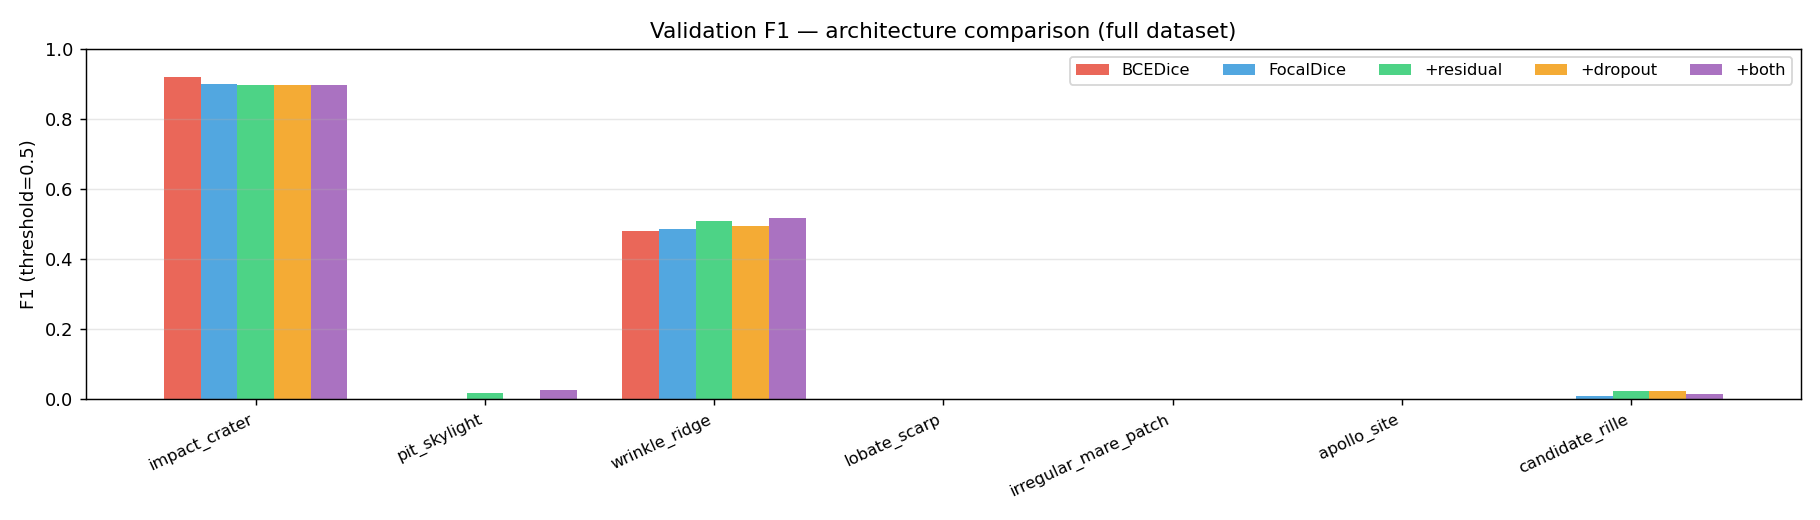
\includegraphics[width=\textwidth]{figures/MR/cloudveneto_arch_val_f1.png}
    \caption{Validation F1}
\end{subfigure}
\hfill
\begin{subfigure}[b]{0.32\textwidth}
    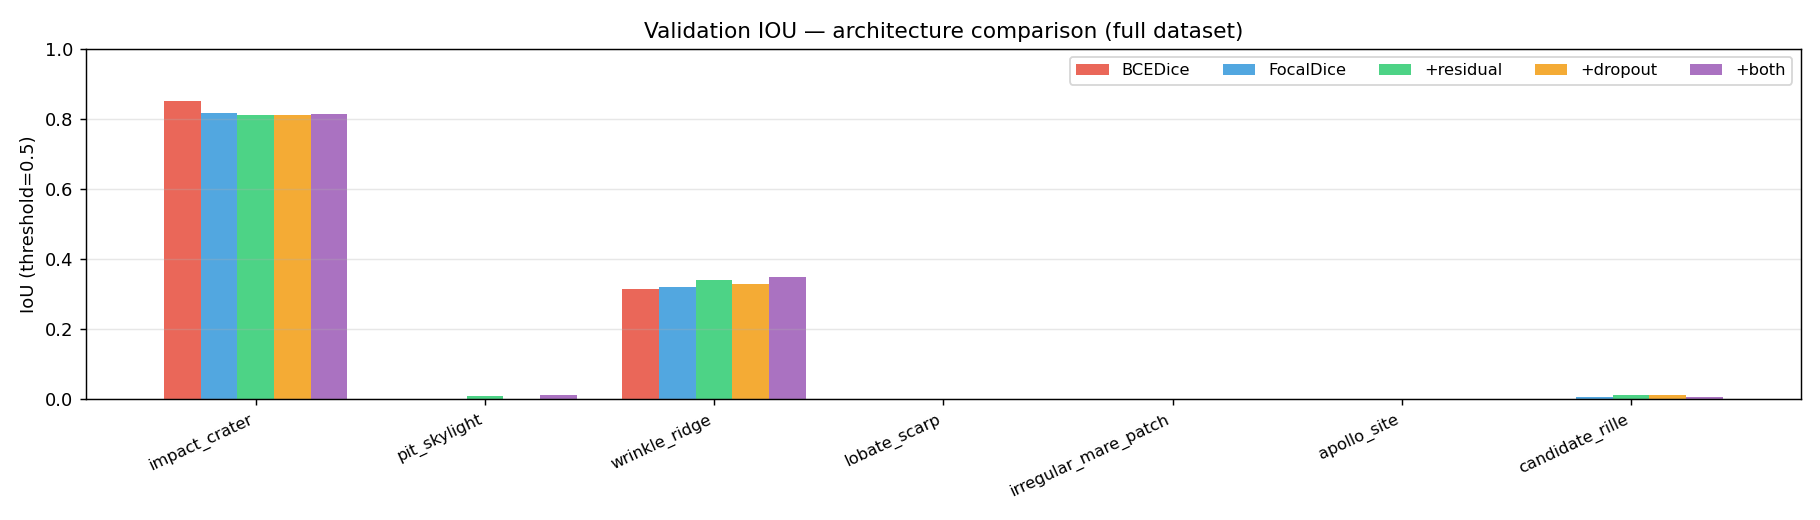
\includegraphics[width=\textwidth]{figures/MR/cloudveneto_arch_val_iou.png}
    \caption{Validation IoU}
\end{subfigure}
\hfill
\begin{subfigure}[b]{0.32\textwidth}
    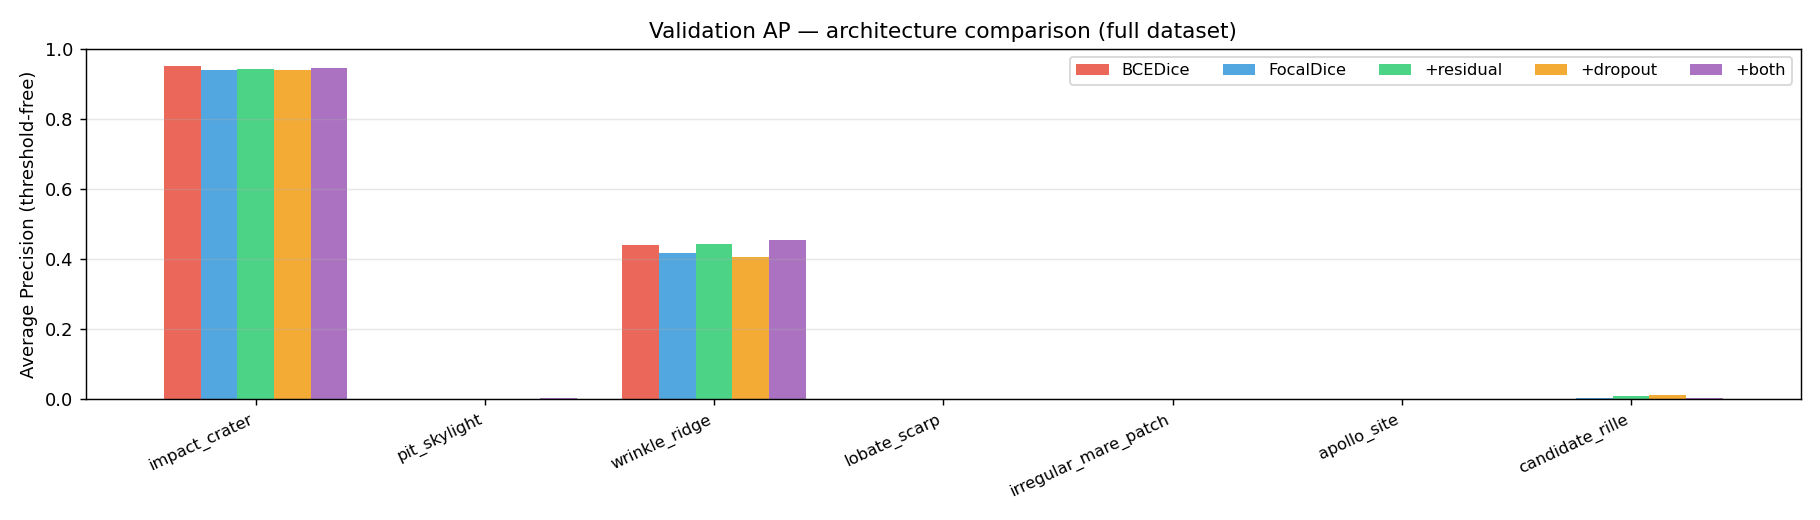
\includegraphics[width=\textwidth]{figures/MR/cloudveneto_arch_val_ap.png}
    \caption{Validation AP}
\end{subfigure}
\caption{Per-class validation metrics across training epochs for the five architecture configurations (full T4 run, 30 epochs). \textbf{+both} (residual + dropout + FocalDice) achieves the highest aggregate performance on all three metrics.}
\label{fig:arch_metrics}
\end{figure}

\paragraph{Key findings.}
Residual shortcuts consistently improve over the plain DoubleConv baseline on aggregate F1, IoU, and AP (+residual vs FocalDice: $+0.0071$ mean F1, $+0.0050$ mean AP). Dropout alone does not help — it degrades both mean AP and ridge AP relative to plain FocalDice, likely because sparse labels already act as a strong regulariser. The combination \textbf{+both} achieves the best mean F1 (0.2076), best mean IoU (0.1688), and best mean AP (0.2004), as well as the highest ridge AP (0.453). Impact-crater AP is uniformly high (0.939–0.951) across all configurations, but given the 0.821 prevalence baseline (Table~\ref{tab:prevalence}) this represents only a modest lift over chance; the architecture choice matters primarily for rare and structurally subtle classes such as ridges, where AP~0.44--0.45 is ${\sim}70\times$ the 0.0064 chance level.

% -----------------------------------------------------------------------------
\subsection{Study 2 — Network Width}
\label{sec:mr_width}

Using the best architecture from Study~1 (\textbf{+both}: FocalDice + residual + dropout=0.3), we sweep the base width $w \in \{16, 32, 64\}$, corresponding to 505K, 2.0M, and 8.0M parameters respectively.

\begin{table}[h]
\centering
\caption{Base-width sweep (FocalDice + residual + dropout=0.3, full T4 run, 30 epochs).}
\label{tab:bw_comparison}
\begin{tabular}{lrrrrrr}
\toprule
Config & Params & Epoch (s) & Mean F1 & Mean IoU & Mean AP & Ridge AP \\
\midrule
small ($w=16$)   &    505{,}095 &  139 & 0.2031 & 0.1665 & 0.2003 & 0.451 \\
default ($w=32$) & 2{,}014{,}727 &  258 & 0.2093 & 0.1704 & 0.2010 & 0.456 \\
wide ($w=64$)    & 8{,}047{,}623 &  582 & \textbf{0.2153} & \textbf{0.1733} & \textbf{0.2016} & 0.445 \\
\bottomrule
\end{tabular}
\end{table}

\begin{figure}[h]
\centering
\begin{subfigure}[b]{0.32\textwidth}
    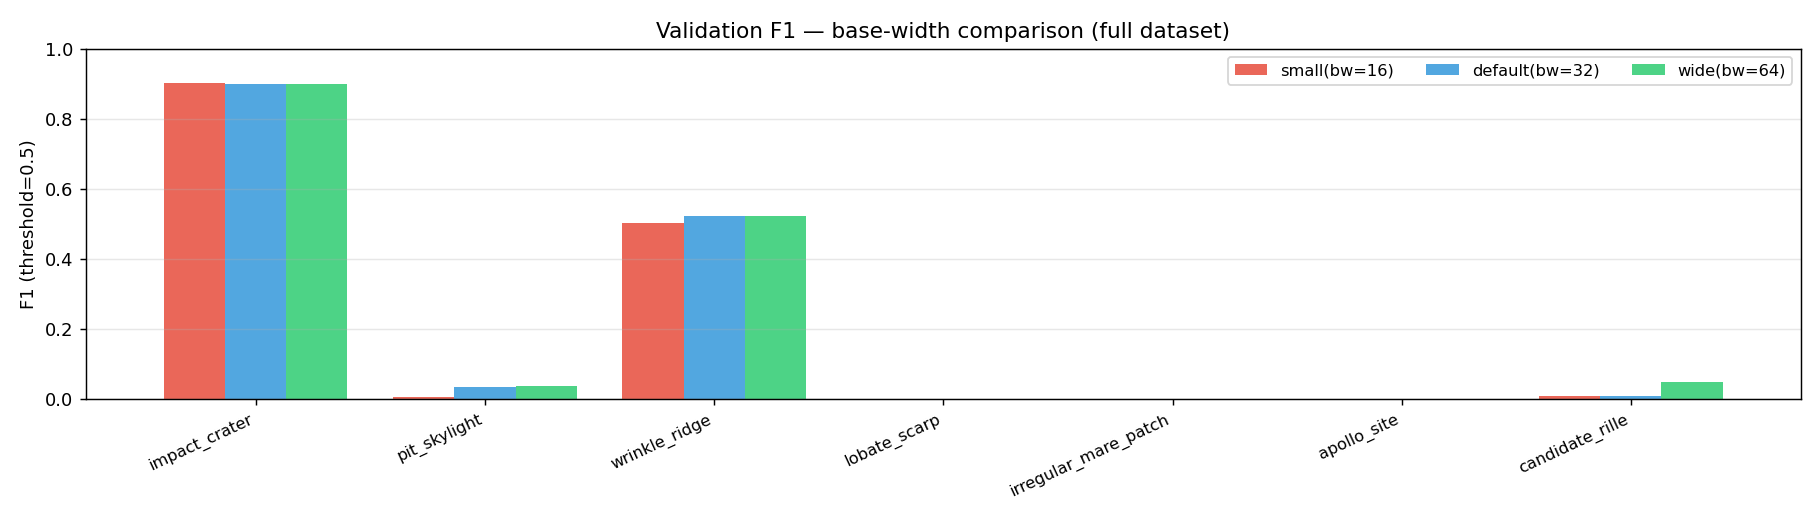
\includegraphics[width=\textwidth]{figures/MR/cloudveneto_bw_val_f1.png}
    \caption{Validation F1}
\end{subfigure}
\hfill
\begin{subfigure}[b]{0.32\textwidth}
    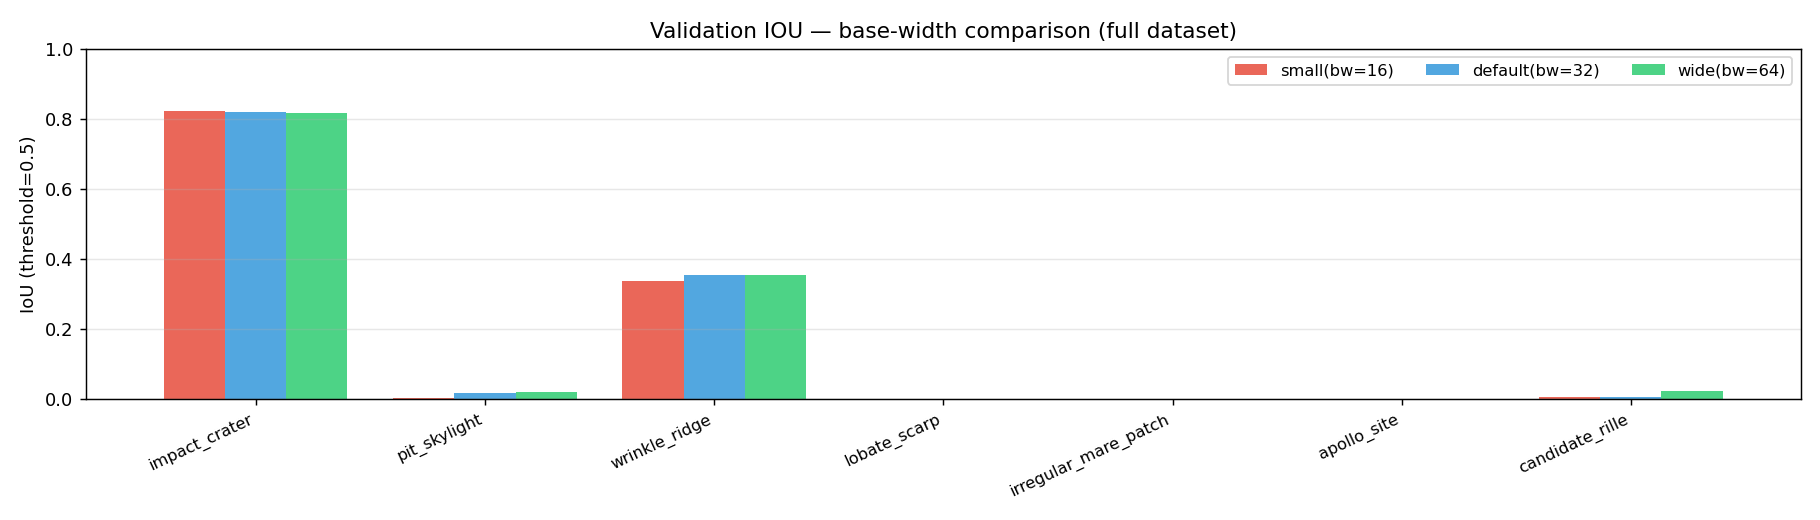
\includegraphics[width=\textwidth]{figures/MR/cloudveneto_bw_val_iou.png}
    \caption{Validation IoU}
\end{subfigure}
\hfill
\begin{subfigure}[b]{0.32\textwidth}
    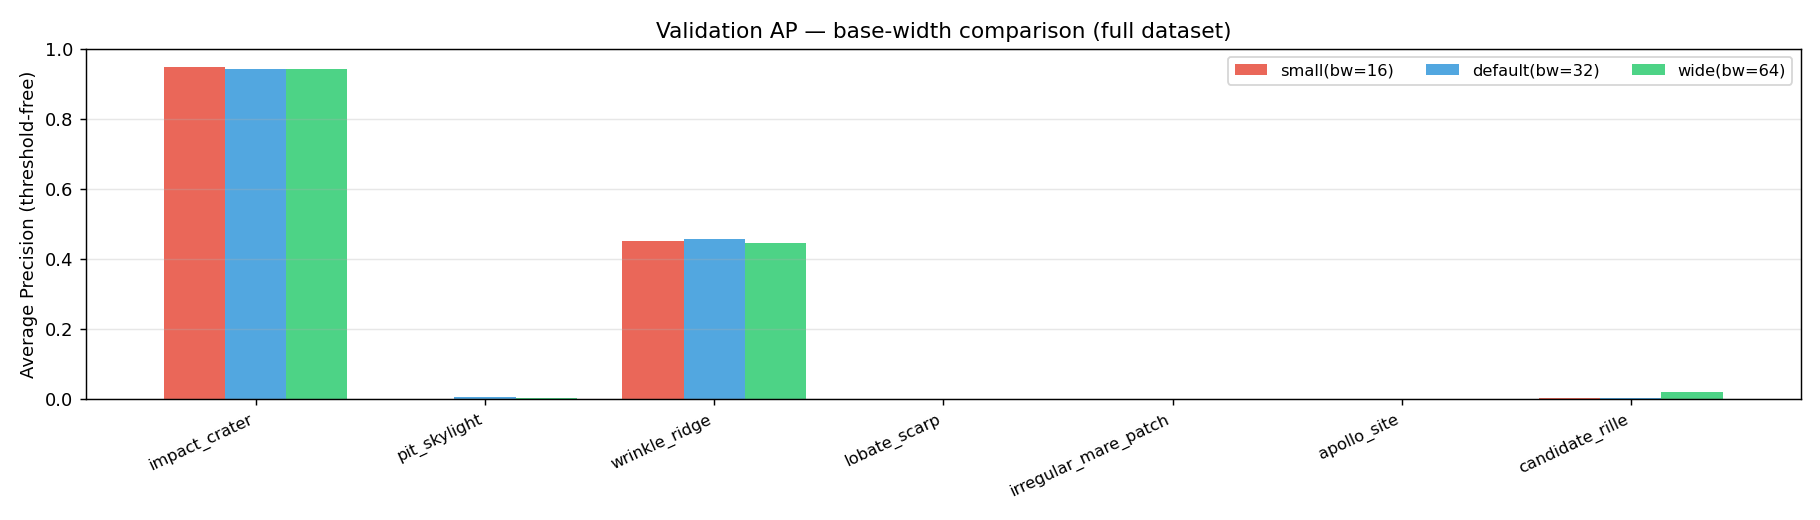
\includegraphics[width=\textwidth]{figures/MR/cloudveneto_bw_val_ap.png}
    \caption{Validation AP}
\end{subfigure}
\caption{Validation metrics for three network widths (full T4 run, 30 epochs). Wider networks achieve marginally higher scores but exhibit severely diminishing returns in terms of parameters and training time.}
\label{fig:bw_metrics}
\end{figure}

\paragraph{Key findings.}
The wide model ($w=64$) achieves the best mean AP (0.2016) and mean F1 (0.2153), but the improvement over the default ($w=32$) is marginal: $+0.0006$ mean AP, $+0.006$ mean F1, at the cost of a 4$\times$ parameter increase and a ${\sim}2.3\times$ increase in training time per epoch (258 s $\to$ 582 s). Strikingly, the small model ($w=16$) with only 505K parameters achieves a mean AP of 0.2003 — within 0.001 of the 8M-parameter wide model — making it the most parameter-efficient option. For deployment on resource-constrained hardware the small model offers the best trade-off.

% -----------------------------------------------------------------------------
\subsection{Study 3 — Data Augmentation}
\label{sec:mr_augmentation}

Using \textbf{+both} at $w=32$, we isolate the effect of geometric augmentation. The augmented pipeline applies random horizontal and vertical flips and 90°/180°/270° rotations to training tiles. No augmentation is applied to validation.

\begin{table}[h]
\centering
\caption{Augmentation study (FocalDice + residual + dropout=0.3, $w=32$, full T4 run, 30 epochs). Crater AP is given for reference; Ridge AP highlights the most affected rare class.}
\label{tab:aug_comparison}
\begin{tabular}{lrrrrrr}
\toprule
Config & Final loss & Mean F1 & Mean IoU & Mean AP & Crater AP & Ridge AP \\
\midrule
\textbf{no augmentation} & \textbf{3.698} & \textbf{0.2986} & \textbf{0.2289} & \textbf{0.2647} & \textbf{0.947} & \textbf{0.558} \\
+augmentation            &        3.863  &        0.2124  &        0.1724  &        0.2027  &        0.942  &        0.457  \\
\bottomrule
\end{tabular}
\end{table}

\begin{figure}[h]
\centering
\begin{subfigure}[b]{0.32\textwidth}
    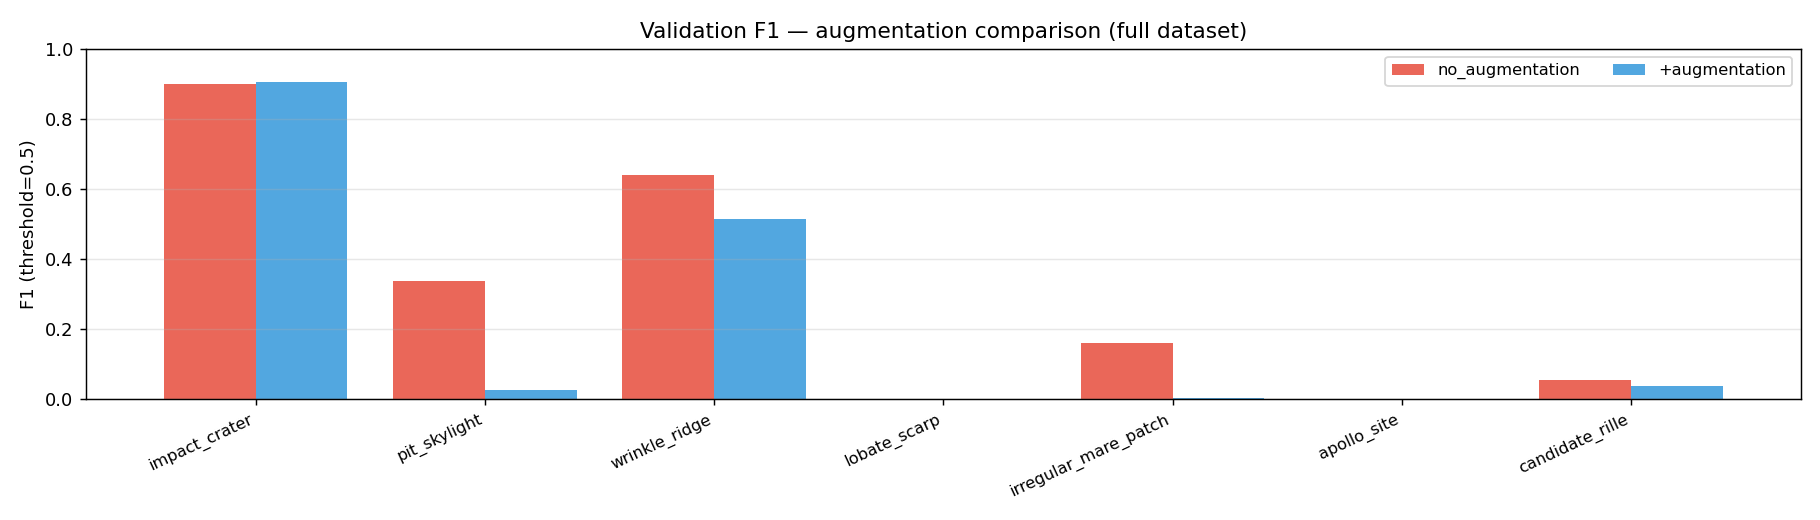
\includegraphics[width=\textwidth]{figures/MR/cloudveneto_aug_val_f1.png}
    \caption{Validation F1}
\end{subfigure}
\hfill
\begin{subfigure}[b]{0.32\textwidth}
    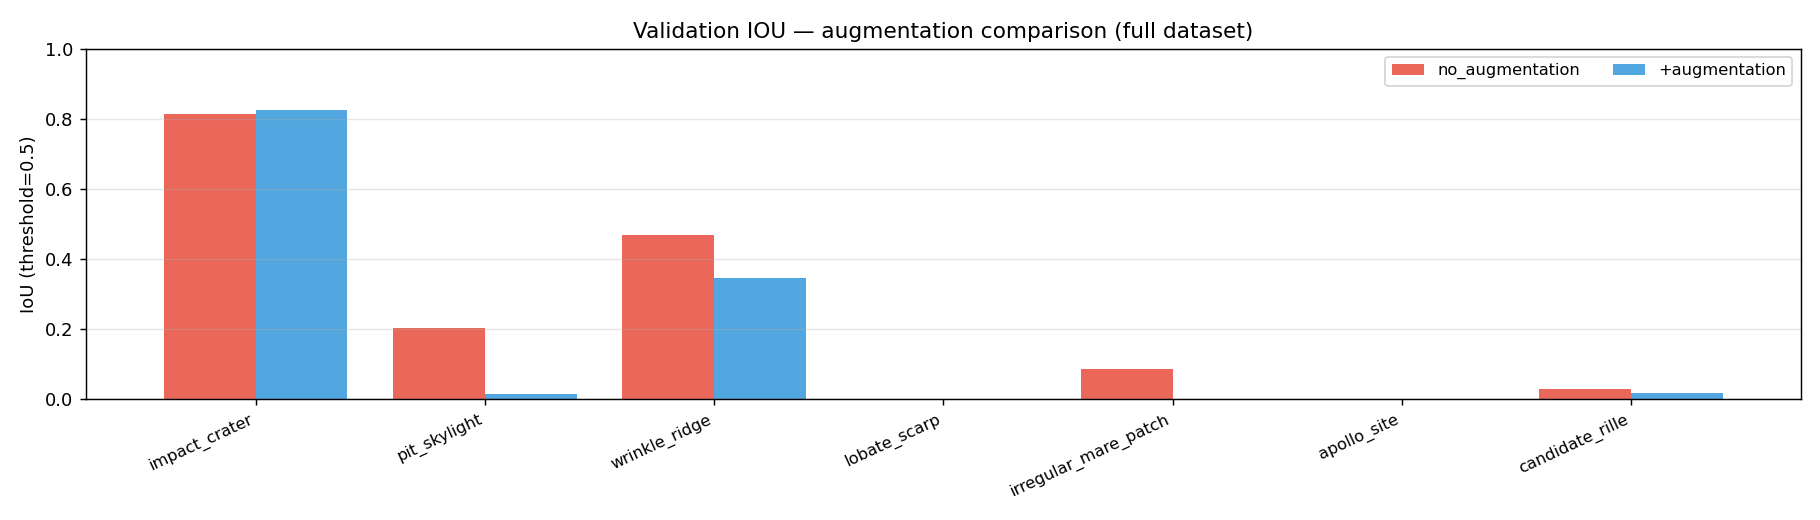
\includegraphics[width=\textwidth]{figures/MR/cloudveneto_aug_val_iou.png}
    \caption{Validation IoU}
\end{subfigure}
\hfill
\begin{subfigure}[b]{0.32\textwidth}
    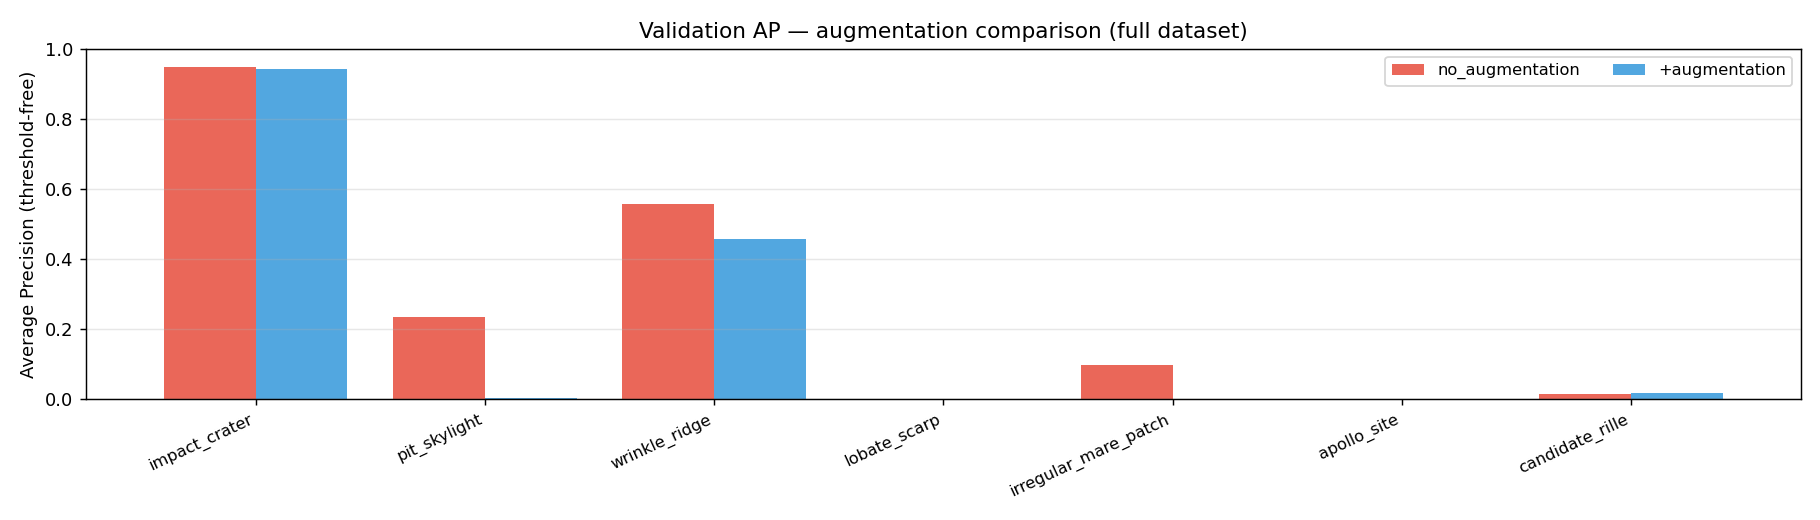
\includegraphics[width=\textwidth]{figures/MR/cloudveneto_aug_val_ap.png}
    \caption{Validation AP}
\end{subfigure}
\caption{Validation metrics with and without geometric augmentation (full T4 run, 30 epochs). No augmentation outperforms the augmented training on all metrics.}
\label{fig:aug_metrics}
\end{figure}

\paragraph{Key findings.}
This is the most striking result of the ablation campaign. Training without augmentation produces a model that is dramatically better on every metric: mean F1 improves by 0.086 (40\% relative), mean AP improves by 0.062 (31\% relative), and ridge AP improves from 0.457 to 0.558 (22\% relative).

Two effects plausibly combine to produce this result, and the present experiment cannot fully separate them.

First, a \emph{geological} effect: the Marius Hills region has a strong directional bias — wrinkle ridges run predominantly in a narrow range of orientations dictated by the regional stress field, and rilles follow the same orientation. Moreover, the Sun azimuth is consistent within the WAC mosaic, so flips and $90°$ rotations also produce illumination directions that never occur in the data. Applying such transforms presents the model with feature orientations and shading that are physically absent in the training region, injecting false diversity. Generic augmentation implicitly assumes that the transformed inputs remain representative of the target distribution~\cite{shorten2019augmentation}, an assumption violated here — the course material itself cautions against ``arbitrary rotations if illumination direction carries physical meaning''~\cite{zingales2026lecture}. Impact craters, being rotationally symmetric, are unaffected, which explains why crater AP is nearly identical in both conditions (0.947 vs 0.942).

Second, a \emph{methodological} confound: as noted in Sec.~\ref{sec:mr_dataset}, the random tile split leaks overlapping pixels into validation. A model trained without augmentation is freer to memorise tile appearance and is rewarded for it on a leaky split, while augmentation suppresses exactly this memorisation. Part of the measured gap could therefore be an artefact of the split rather than a property of the data. To separate the two effects, the comparison was re-run under the leakage-free spatial block split.

\paragraph{Leakage-free re-run.}
The augmentation pair was re-trained with \texttt{spatial\_train\_val\_split}: both arms share an identical pixel-disjoint split, the same initialisation seed, and the same cosine schedule, so the \emph{only} difference between them is augmentation. The re-run used a scaled paired protocol on local hardware (10{,}000 tiles, 30 epochs; a paired comparison remains internally valid at reduced scale), with a smaller 6{,}000-tile/15-epoch run giving consistent results. Table~\ref{tab:spatial_rerun} and Figure~\ref{fig:spatial_rerun} report the outcome.

\begin{table}[h]
\centering
\caption{Augmentation ablation under the leakage-free spatial split (10{,}000 tiles, 30 epochs, paired arms). \texttt{candidate\_rille} has zero positive pixels in the spatial validation set and is excluded from the macro averages (reported as NaN with zero support).}
\label{tab:spatial_rerun}
\begin{tabular}{lrrrr}
\toprule
Config & Mean F1 & Mean AP & Ridge F1 & Ridge AP \\
\midrule
\textbf{no augmentation} & \textbf{0.2294} & \textbf{0.2239} & \textbf{0.4586} & \textbf{0.3847} \\
+augmentation            &        0.2208  &        0.2096  &        0.3970  &        0.3060  \\
\bottomrule
\end{tabular}
\end{table}

\begin{figure}[h]
\centering
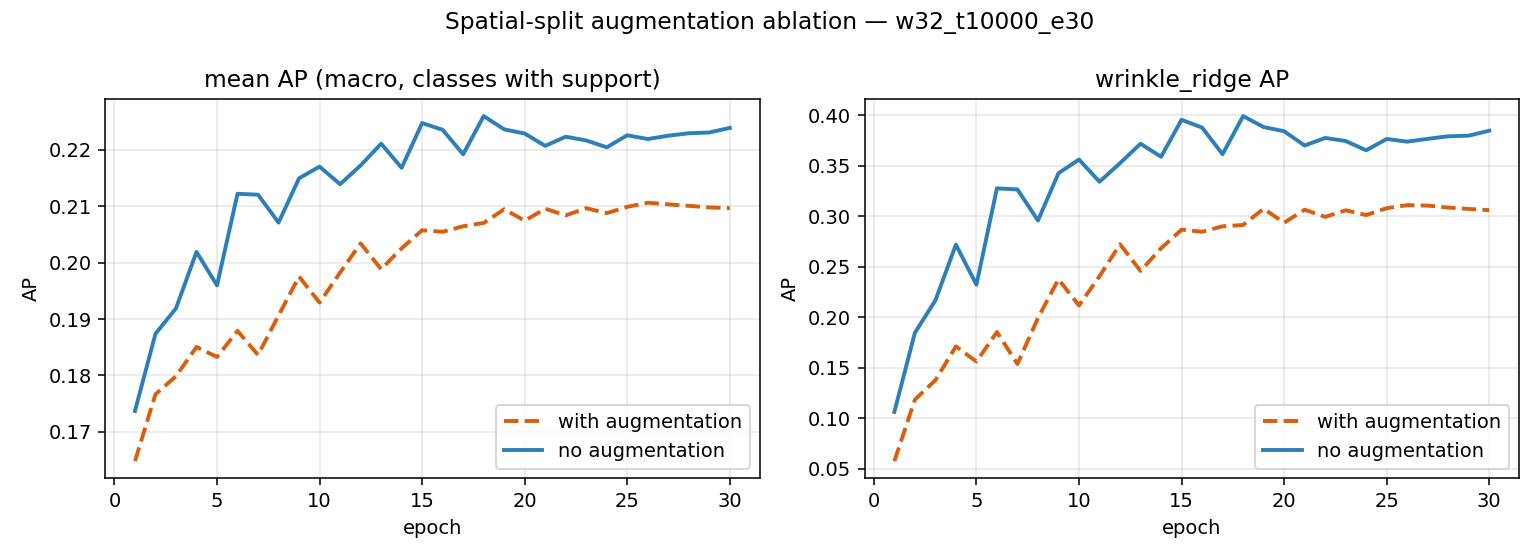
\includegraphics[width=\textwidth]{figures/MR/spatial_w32_t10000_e30_val_ap.png}
\caption{Validation AP across training epochs under the spatial split (macro mean over classes with support, left; \texttt{wrinkle\_ridge}, right). The no-augmentation arm dominates at every epoch on both metrics.}
\label{fig:spatial_rerun}
\end{figure}

The re-run \textbf{confirms the conclusion}: training without augmentation remains better, with the no-augmentation arm above the augmented one at every epoch (Fig.~\ref{fig:spatial_rerun}). The decomposition is, however, instructive. Absolute scores are substantially lower than on the leaky split (ridge AP 0.385 vs 0.558), confirming that random-split numbers were inflated by memorisation. The \emph{aggregate} advantage of no-augmentation also narrows (mean AP $+0.014$ here vs $+0.062$ on the leaky split), showing that part of the originally measured gap was indeed a split artefact. But for the direction-sensitive class the gap persists and is large — ridge AP 0.385 vs 0.306, a 26\% relative difference on strictly disjoint validation pixels — which is precisely the signature predicted by the geological explanation: augmentation hurts where orientation and illumination carry physical information. Confirmation at the full 15{,}931-tile T4 protocol remains scheduled, but the conclusion no longer rests on a confounded measurement.

% -----------------------------------------------------------------------------
\subsection{Qualitative Evaluation}
\label{sec:mr_qualitative}

Segmentation metrics alone do not reveal \emph{how} a model fails, so we complement the ablations with a visual comparison on identical validation tiles: raw image, ground truth, predicted probability, and a true-positive/false-positive/false-negative decomposition at threshold $0.5$, for the BCEDice baseline and the definitive model side by side (generated by \texttt{scripts/qualitative\_eval.py}; tiles are the three validation tiles with the largest \texttt{wrinkle\_ridge} ground-truth area).

\begin{figure}[h]
\centering
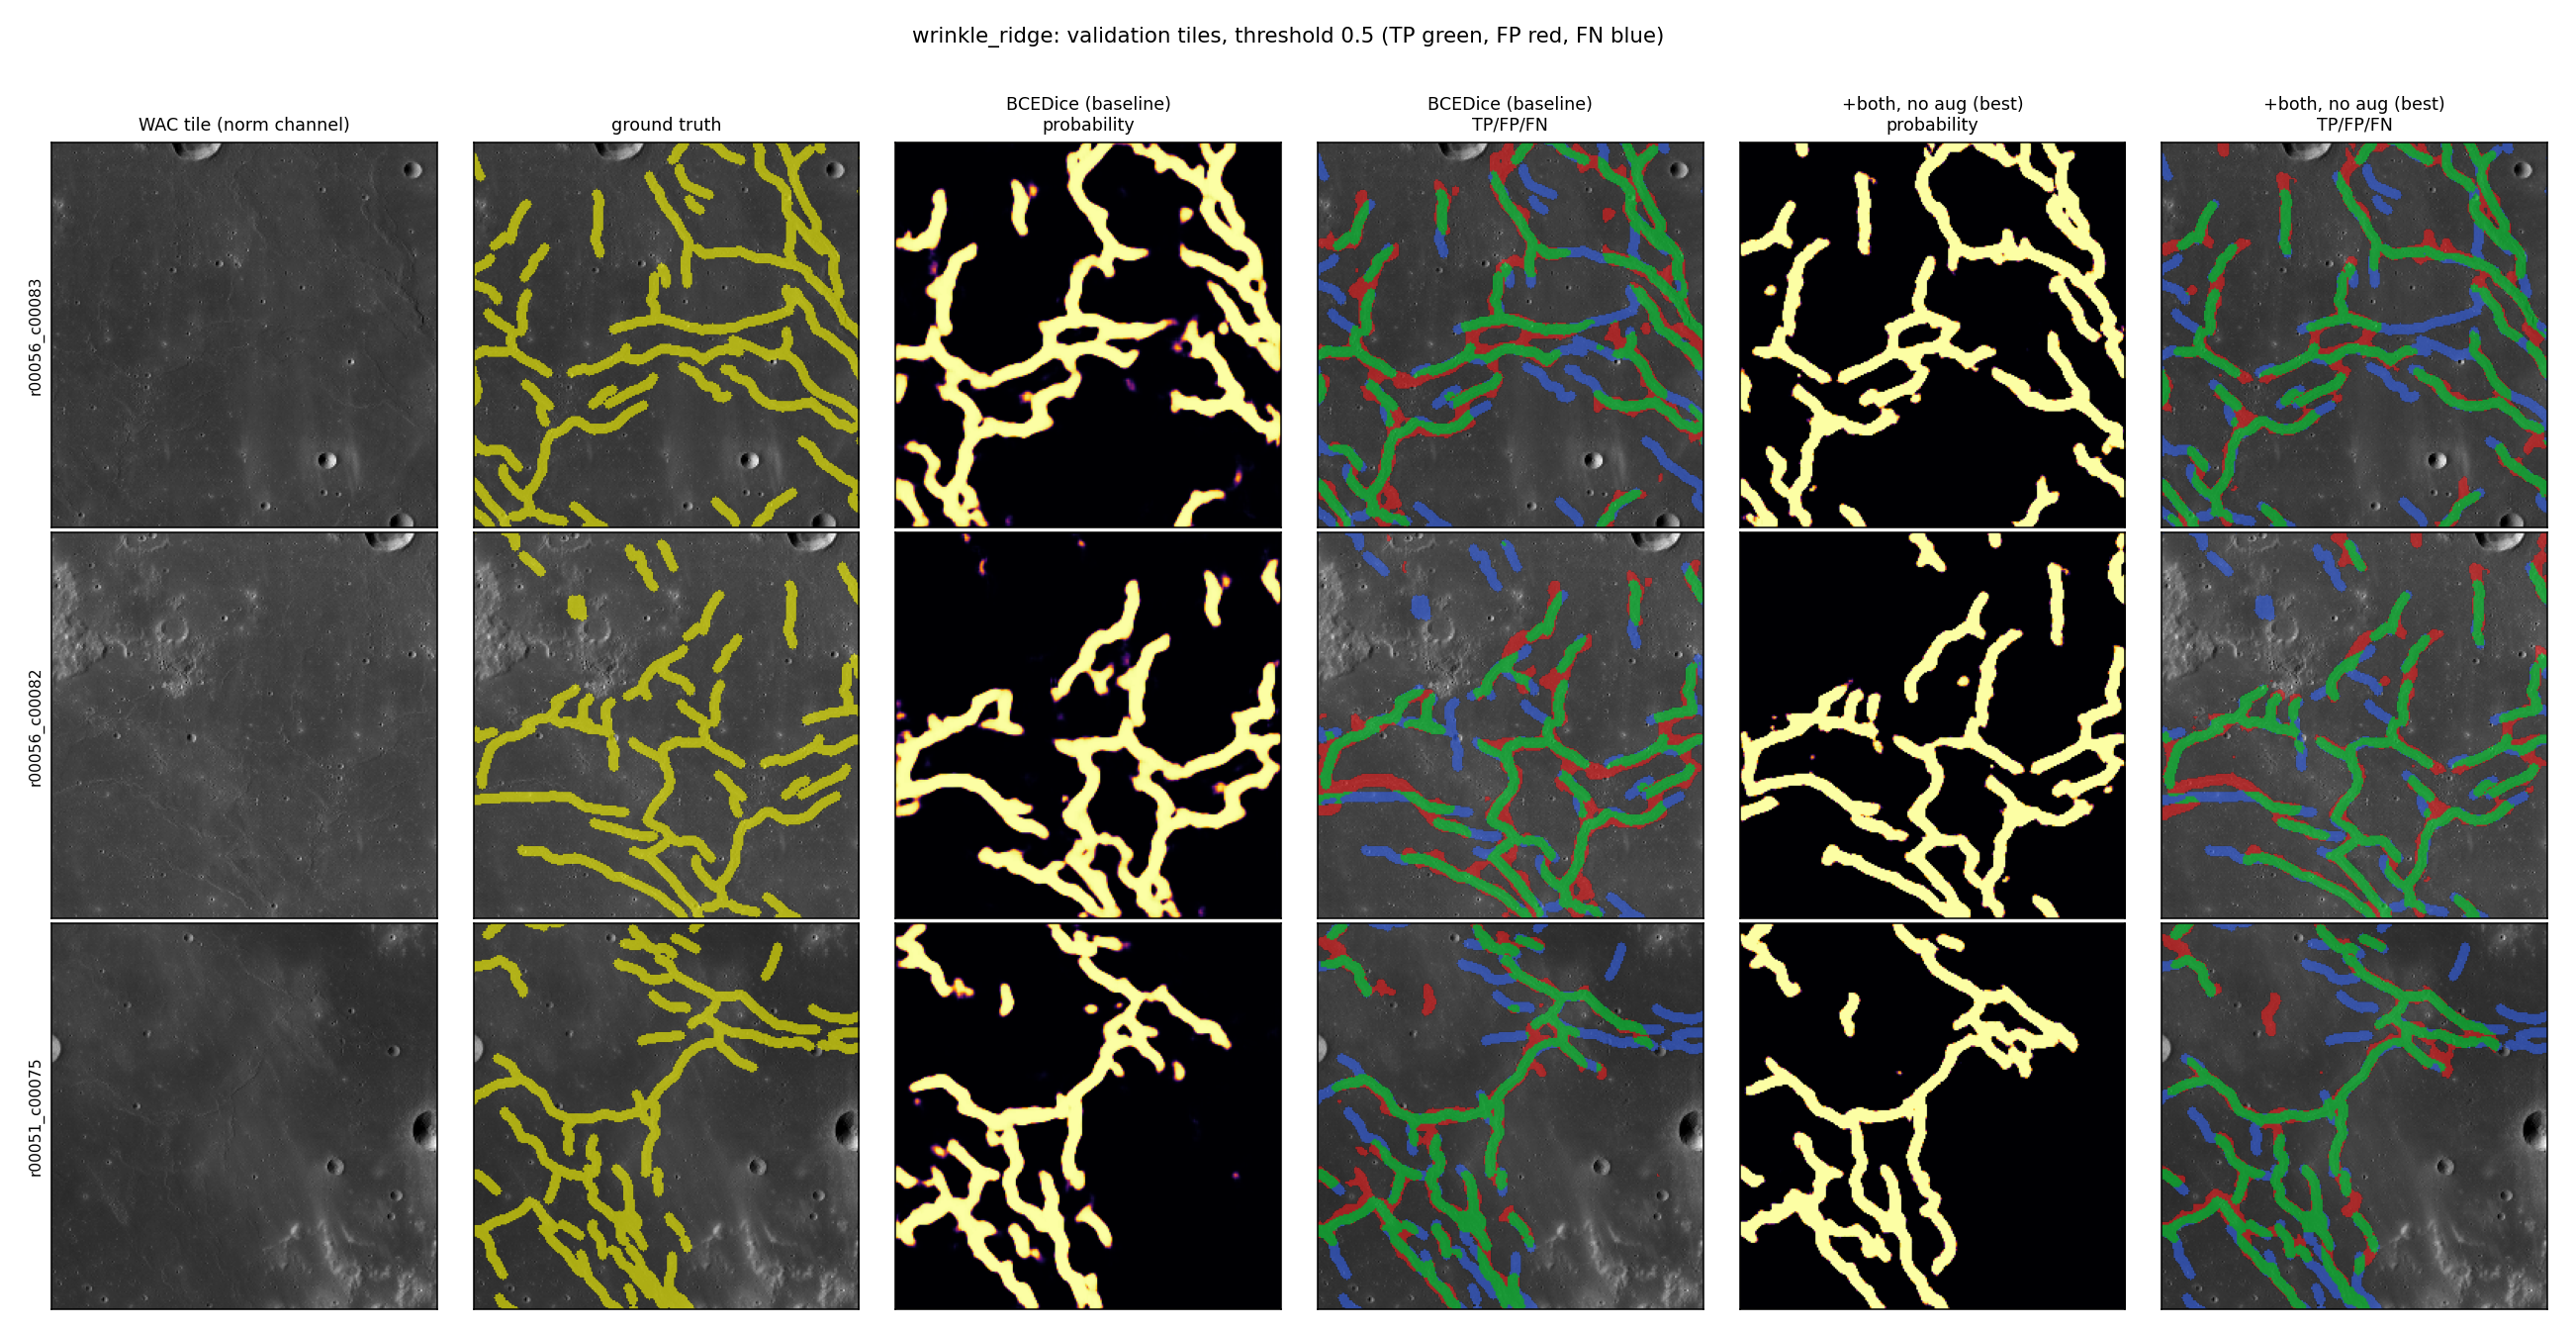
\includegraphics[width=\textwidth]{figures/MR/qualitative_wrinkle_ridge.png}
\caption{Wrinkle-ridge qualitative comparison on three validation tiles (TP green, FP red, FN blue). Both models recover the topology of the ridge network; the definitive model (+both, no augmentation) produces visibly more complete coverage and fewer false positives than the BCEDice baseline. Errors concentrate on thin, low-contrast ridge segments, consistent with the localisation difficulty of linear features.}
\label{fig:qualitative_ridge}
\end{figure}

\begin{figure}[h]
\centering
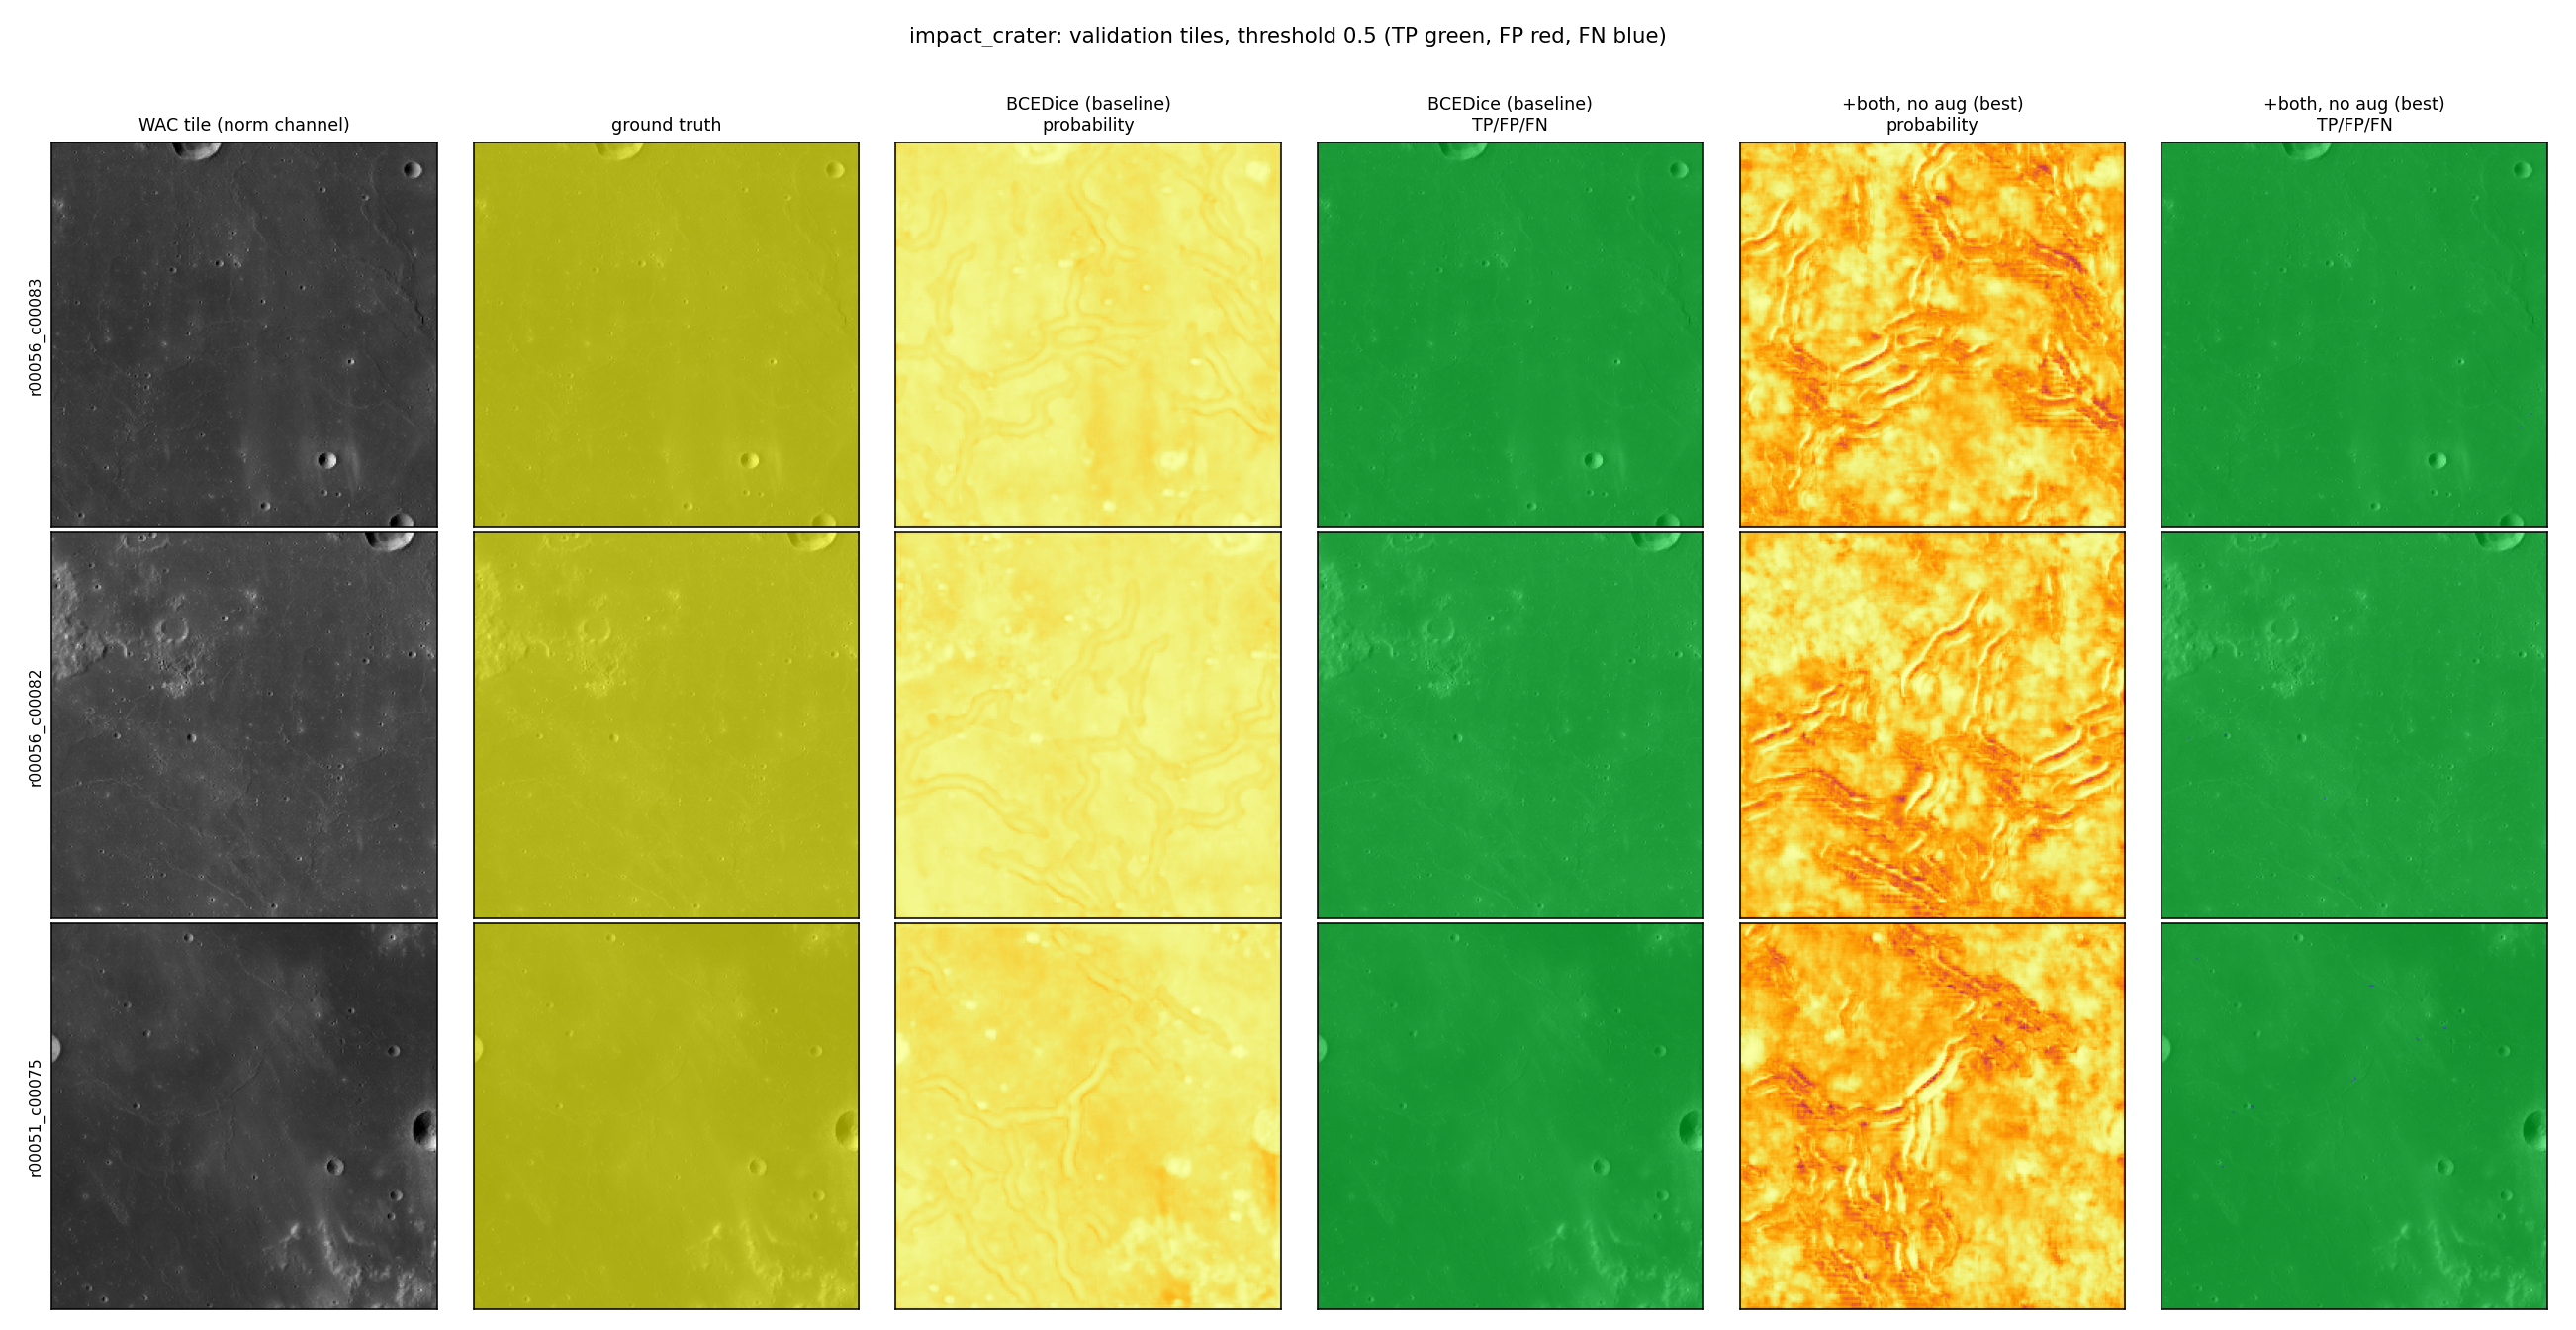
\includegraphics[width=\textwidth]{figures/MR/qualitative_impact_crater.png}
\caption{Impact-crater qualitative comparison on the same tiles. The ground truth covers the \emph{entire} tile (cf.\ the 82\% prevalence and 50.7\% fully-covered tiles of Table~\ref{tab:prevalence}), so a prediction of ``everywhere'' is trivially correct: this figure is direct visual evidence that the crater channel behaves as a near-coverage layer and that crater AP must be read against its 0.821 chance baseline.}
\label{fig:qualitative_crater}
\end{figure}

The ridge comparison shows that the metric gains of the definitive model correspond to a real, visible improvement in completeness of the recovered ridge network. The crater comparison, conversely, makes the saturation argument of Sec.~\ref{sec:mr_dataset} concrete.

% -----------------------------------------------------------------------------
\subsection{South Pole Inference}
\label{sec:mr_south_pole}

The best-performing model weights (\texttt{best\_trained.pth}) were applied to the lunar south pole to demonstrate transfer beyond the training region. The south pole imagery was obtained from the same LRO WAC source and tiled identically, producing 3{,}639 tiles.

\paragraph{Inference pipeline.}
Each tile is preprocessed with the same CLAHE + Sobel three-channel pipeline. A sliding-window predictor runs the model tile by tile, saving per-class probability maps as compressed \texttt{.npz} files for downstream aggregation. Probability maps are aggregated over all tiles to compute global statistics.

\paragraph{Per-class results.}
Table~\ref{tab:south_pole_stats} reports the aggregated statistics over the 3{,}639 south pole tiles.

\begin{table}[h]
\centering
\caption{South pole inference results (3{,}639 tiles). Avg.\ Max.\ Prob.\ is the mean, over tiles, of the maximum predicted probability for each class. Global Max is the highest probability observed in any single tile. A high avg.\ max but low global max indicates diffuse, uncertain detections; a high global max but low avg.\ max indicates rare but confident detections.}
\label{tab:south_pole_stats}
\begin{tabular}{lrrr}
\toprule
Class & Avg.\ Max.\ Prob. & Global Max & Status \\
\midrule
\texttt{impact\_crater}       & 0.863 & 1.000 & \checkmark\ detected \\
\texttt{lobate\_scarp}        & 0.060 & 0.303 & weak \\
\texttt{pit\_skylight}        & 0.051 & 0.202 & weak \\
\texttt{irregular\_mare\_patch} & 0.040 & 0.215 & weak \\
\texttt{apollo\_site}         & 0.040 & 0.183 & weak \\
\texttt{candidate\_rille}     & 0.006 & 0.480 & sparse \\
\texttt{wrinkle\_ridge}       & 0.001 & 1.000 & sparse \\
\bottomrule
\end{tabular}
\end{table}

\begin{figure}[h]
\centering
\begin{subfigure}[b]{0.48\textwidth}
    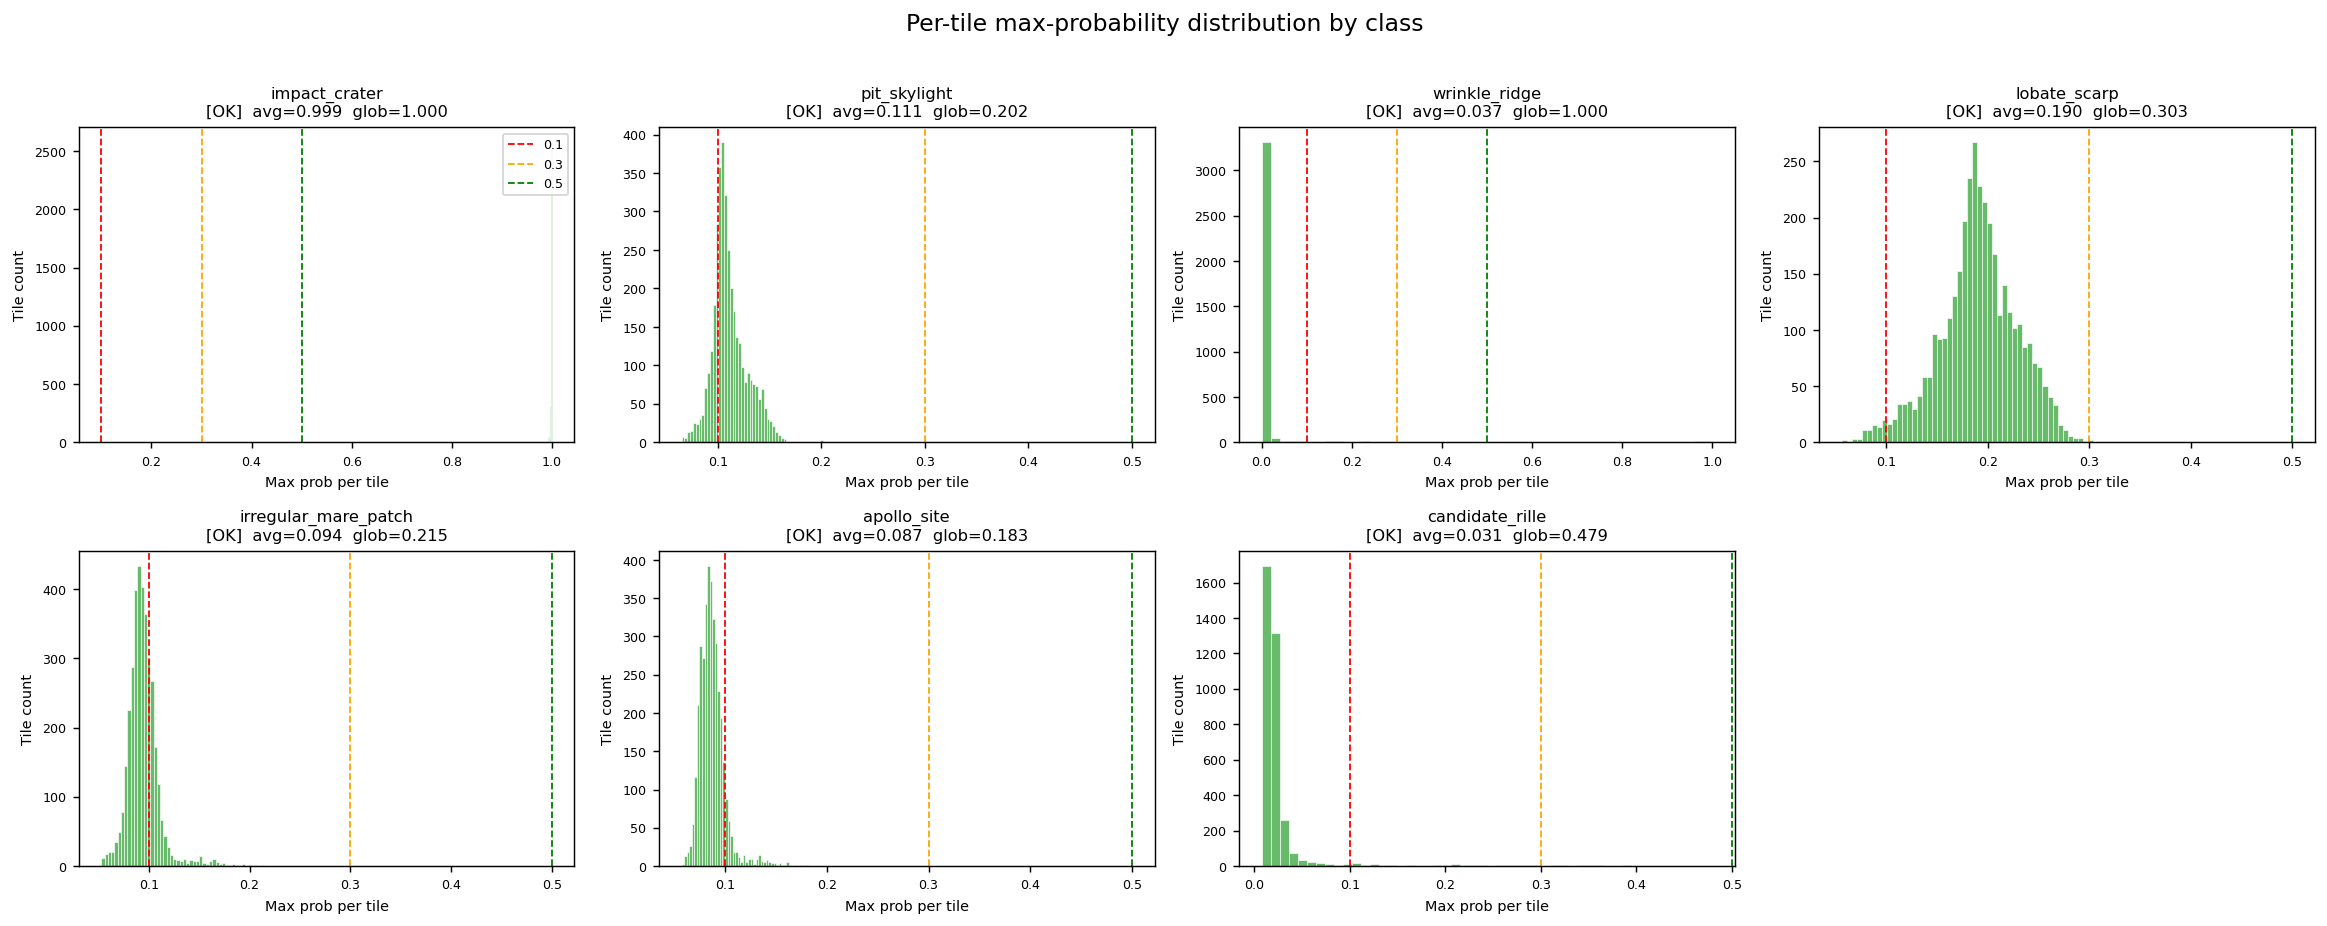
\includegraphics[width=\textwidth]{figures/MR/diagnostics_distributions.png}
    \caption{Per-tile max-probability distributions.}
\end{subfigure}
\hfill
\begin{subfigure}[b]{0.48\textwidth}
    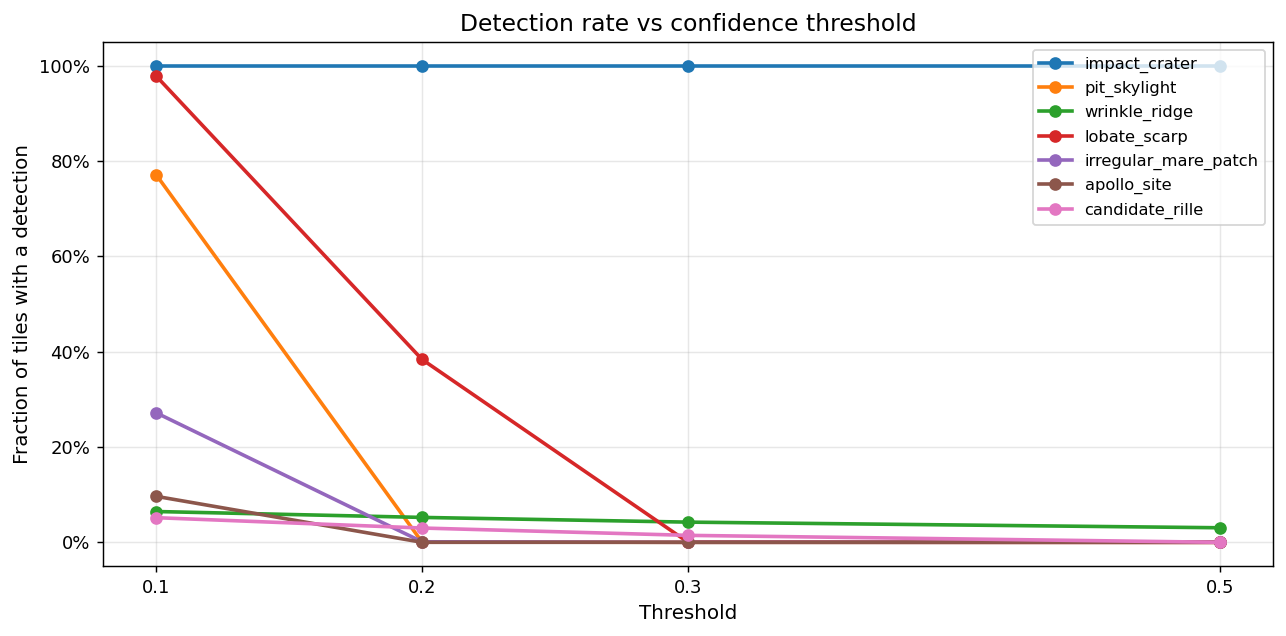
\includegraphics[width=\textwidth]{figures/MR/diagnostics_detection_rates.png}
    \caption{Detection rate vs.\ confidence threshold.}
\end{subfigure}
\caption{South pole inference diagnostics across 3{,}639 tiles. Impact craters are detected with near-certainty across the entire region. All other classes exhibit strongly right-skewed distributions with low average confidence, reflecting both the domain shift from Marius Hills and the scarcity of these features at the south pole.}
\label{fig:south_pole_diag}
\end{figure}

\begin{figure}[h]
\centering
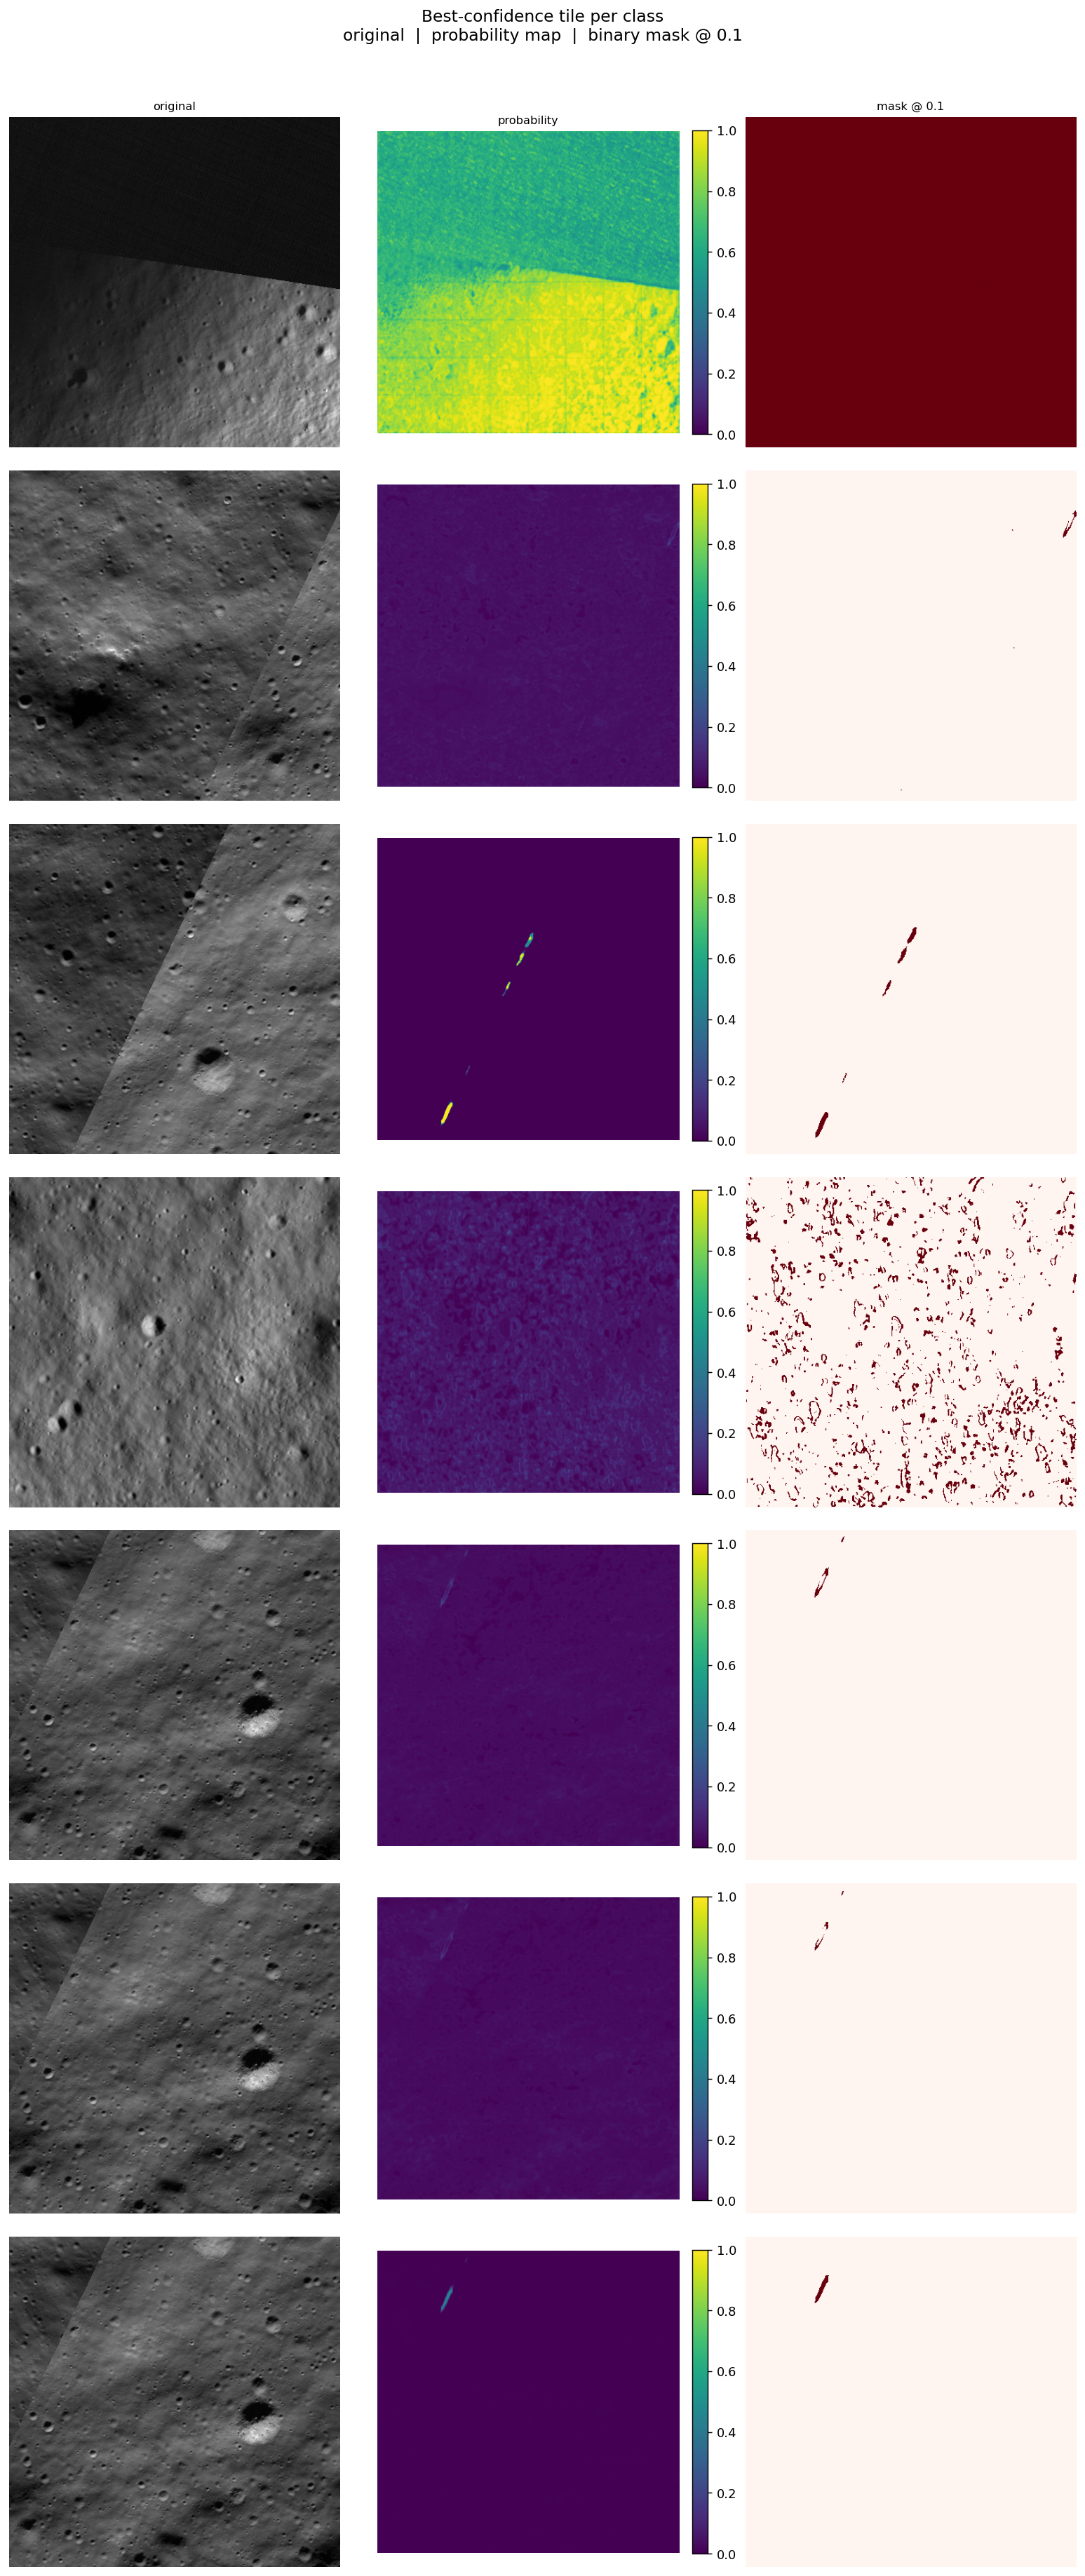
\includegraphics[width=\textwidth, height=0.82\textheight, keepaspectratio]{figures/MR/diagnostics_best_tiles.png}
\caption{Best-detected tile per class on the south pole imagery. Each panel shows the LRO WAC tile overlaid with the predicted probability map for the class with the highest maximum confidence in that tile. Note that overlays use a \emph{relative} threshold (top fraction of each tile's probabilities) so that the most likely candidate pixels are visible even when absolute confidence is low; coloured regions for the weak classes are therefore candidate locations, not confident detections. Impact craters stand out clearly; other classes show localised but low-confidence activations.}
\label{fig:south_pole_best}
\end{figure}

\paragraph{Analysis.}
The model assigns high crater probability across the entire south pole (average max probability 0.863). Given the near-saturated crater layer learned in training (Sec.~\ref{sec:mr_dataset}), this is expected behaviour — the model has learned that almost everywhere is ``crater'' — and should not be over-interpreted as precise crater delineation. Two classes — \texttt{wrinkle\_ridge} and \texttt{candidate\_rille} — show an interesting pattern: very low average-tile probabilities (0.001 and 0.006) but anomalously high global maxima (1.000 and 0.480). This indicates that the model makes rare but high-confidence predictions on a small number of tiles, rather than diffuse low-confidence activations everywhere.

The weak performance on rare classes at the south pole is attributable to two combined factors. First, the south pole is geologically distinct from Marius Hills: it lacks the volcanic structures (skylights, rilles, ridges) that dominate the training distribution, making it an out-of-distribution region for those classes. Second, the extremely low frequency of those classes in the training data means the model has seen very few positive examples even during Marius Hills training. Both issues motivate future work on label-efficient transfer learning and domain adaptation.

% -----------------------------------------------------------------------------
\subsection{Methodological Audit and Reproducibility}
\label{sec:mr_audit}

After the experimental campaign was completed, the entire pipeline — code, data, report claims, and course guidance — was subjected to a systematic audit. Every resulting change is a single, individually justified commit on the \texttt{U-net} branch, indexed in \texttt{Moon-Recognition/IMPROVEMENTS.md}; the executed notebooks were committed \emph{before} any fix, so the provenance of the published numbers is preserved. This section summarises what the audit found and how each finding affects the interpretation of the results — both as a record for the group and because several findings changed the conclusions of this report.

\paragraph{(a) Report--code reconciliation.}
Several statements in an earlier draft did not match the implementation and were corrected against the code as ground truth: the CLAHE parameters (the pipeline uses \texttt{skimage} \texttt{equalize\_adapthist} with clip limit 0.03, not the OpenCV-style values previously quoted), the tiling description (tiles \emph{overlap} by 50\%), the split procedure (random permutation, not sequential), a gradient-clipping claim (clipping was never enabled), and a mis-attributed citation in the augmentation discussion (replaced with the correct survey~\cite{shorten2019augmentation}). The principle applied: any claim an examiner can check against the repository must be checkable.

\paragraph{(b) Train/validation leakage --- discovery and remedy.}
Because adjacent tiles share 50\% of their pixels, the random tile-level split leaks: a direct measurement on the real index showed that \textbf{100\% of the 3{,}186 validation tiles overlap at least one training tile}. This inflates absolute validation scores and specifically confounds the augmentation study, since a non-augmented model is freer to memorise tile appearance and a leaky validation set rewards exactly that memorisation. The remedy, recommended by the course material itself, is a \emph{spatial block split}: contiguous $1024$-px blocks are assigned to validation and every training tile whose footprint intersects a validation tile is discarded ($\texttt{data/splits.py}$; on the real index: 11{,}289 train / 3{,}248 validation tiles, 1{,}394 boundary tiles dropped, zero pixel overlap, verified by an independent assertion). The augmentation comparison was re-run under this split as a scaled paired protocol on local hardware (both arms share an identical split, initialisation, and schedule, so the comparison is internally valid); the conclusion was confirmed, with the expected partial decomposition into a leakage artefact and a genuine effect (Sec.~\ref{sec:mr_augmentation}). Full-protocol confirmation on CloudVeneto remains scheduled when GPU instances become available.

\paragraph{(c) Label audit --- channel saturation.}
A full pass over all 15{,}931 tiles produced the per-class prevalences of Table~\ref{tab:prevalence} and the central reinterpretation of this report: the \texttt{impact\_crater} channel covers 82.1\% of all pixels, making it a near-coverage layer whose AP must be read against a 0.821 chance baseline, while \texttt{wrinkle\_ridge} (prevalence $6.4\times10^{-3}$) emerges as the strongest genuine result and the five rarest classes turn out to have essentially no supervision at all. Without this audit, the headline claim of the report would have been the (nearly trivial) crater result.

\paragraph{(d) Qualitative evaluation.}
The course material requires visual evaluation alongside metrics. Figures~\ref{fig:qualitative_ridge} and~\ref{fig:qualitative_crater} (generated by \texttt{scripts/qualitative\_eval.py} from the full-run checkpoints) confirm both audit findings visually: the metric advantage of the definitive model corresponds to a visibly more complete ridge reconstruction, and the crater ground truth fills entire tiles.

\paragraph{(e) Engineering fixes.}
The audit also produced functional fixes, each preserving the published numbers: evaluation memory reduced by ${\sim}12$\,GB with results verified bit-identical; undefined metrics for classes absent from a validation split now reported as NaN with an explicit support count rather than as a spurious 0; checkpoint loading made compatible with PyTorch $\geq 2.6$ and made loud on architecture/checkpoint mismatches (previously a mismatch silently produced random predictions); the sliding-window inference default aligned with the 256-px training context; dead machine-specific paths removed from the data manifest; and the training configuration file synchronised with the protocol actually used for the published runs.

% -----------------------------------------------------------------------------
\subsection{Summary and Conclusions}
\label{sec:mr_conclusions}

Table~\ref{tab:final_summary} collects the final T4 results for the best configuration identified in each study. The definitive model for the project is \textbf{SmallUNet with $w=32$, FocalDice loss, residual shortcuts, bottleneck dropout ($p=0.3$), trained without augmentation for 30 epochs on the full 15{,}931-tile Marius Hills dataset}. Its weights are stored as \texttt{data/MR/weights/best\_trained.pth}.

\begin{table}[h]
\centering
\caption{Best result from each ablation study (full T4 run, 30 epochs).}
\label{tab:final_summary}
\begin{tabular}{llrrrr}
\toprule
Study & Best config & Params & Mean F1 & Mean AP & Ridge AP \\
\midrule
Architecture & +both ($w=32$, augmented) & 2.0M & 0.2076 & 0.2004 & 0.453 \\
Width        & wide ($w=64$, augmented)  & 8.0M & 0.2153 & 0.2016 & 0.445 \\
Augmentation & +both, $w=32$, \textbf{no aug} & 2.0M & \textbf{0.2986} & \textbf{0.2647} & \textbf{0.558} \\
\bottomrule
\end{tabular}
\end{table}

The principal conclusions of this study are:

\begin{enumerate}
    \item \textbf{Residual shortcuts help; dropout alone does not.} Adding residual connections to DoubleConv blocks consistently improves all aggregate metrics. Bottleneck dropout in isolation hurts performance, likely because sparse labels already regularise the network. The combination \textbf{+both} yields the best augmented-training result.

    \item \textbf{Network width exhibits strong diminishing returns.} The small model ($w=16$, 505K parameters) achieves a mean AP within 0.001 of the wide model ($w=64$, 8M parameters) at one-sixth the training time and ${\sim}16\times$ fewer parameters. For resource-constrained inference the small model is recommended.

    \item \textbf{Geometric augmentation is harmful on this dataset — confirmed under a leakage-free split.} Training without flips and rotations outperforms the augmented model on the original random split, and the advantage survives the spatial block split re-run with strictly disjoint validation pixels (ridge AP 0.385 vs 0.306, no-augmentation above at every epoch). The decomposition is informative: part of the aggregate gap on the random split was a leakage artefact, but the direction-sensitive classes retain a large genuine gap, exactly as predicted by the directional bias of the Marius Hills linear features and the fixed illumination geometry. Augmentation strategies must be tailored to the structural properties of the target domain.

    \item \textbf{Crater AP must be read against its prevalence baseline; ridges are the strongest genuine result.} The \texttt{impact\_crater} channel covers 82.1\% of all pixels (half of the tiles are fully positive), so its AP $\approx 0.95$ is only a modest lift over the 0.821 chance level — the channel behaves as a near-coverage layer, and Fig.~\ref{fig:qualitative_crater} shows that predicting ``everywhere'' is trivially correct. By contrast, \texttt{wrinkle\_ridge} has a prevalence of $6.4\times10^{-3}$, so the best ridge AP of 0.558 is ${\sim}90\times$ chance level and corresponds to a visibly accurate reconstruction of the ridge network (Fig.~\ref{fig:qualitative_ridge}). The remaining five classes have prevalences below $1.4\times10^{-4}$ — their near-zero scores reflect the absence of supervision, not a failure of the architecture.

    \item \textbf{South pole transfer is limited by domain shift and label scarcity.} The model accurately maps impact craters but provides only weak signals for rarer geomorphological features. Acquiring labels for even a small number of south-pole-specific tiles, or employing few-shot domain adaptation, is likely necessary for reliable multi-class south-pole mapping.
\end{enumerate}

% Bibliography entries to add to the main .bib file:
% @inproceedings{ronneberger2015unet,
%   title={U-Net: Convolutional Networks for Biomedical Image Segmentation},
%   author={Ronneberger, Olaf and Fischer, Philipp and Brox, Thomas},
%   booktitle={MICCAI},
%   year={2015}
% }
% @inproceedings{lin2017focal,
%   title={Focal Loss for Dense Object Detection},
%   author={Lin, Tsung-Yi and Goyal, Priya and Girshick, Ross and He, Kaiming and Dollár, Piotr},
%   booktitle={ICCV},
%   year={2017}
% }
% @misc{zingales2026lecture,
%   author={Zingales, Tiziano},
%   title={Moon Features Recognition (Lecture 3b)},
%   howpublished={Computational Physics, Physics of Data, University of Padova},
%   year={2026}
% }
% @article{shorten2019augmentation,
%   title={A survey on Image Data Augmentation for Deep Learning},
%   author={Shorten, Connor and Khoshgoftaar, Taghi M.},
%   journal={Journal of Big Data},
%   volume={6},
%   number={1},
%   pages={60},
%   year={2019}
% }
